%\documentclass[12pt,openright,twoside,a4paper,chapter=TITLE,english]{USPSC}
%\documentclass[12pt,openright,twoside,a4paper,english,sumario=tradicional]{USPSC}
\documentclass[12pt,openright,twoside,a4paper,english]{USPSC}

% ---
% Pacotes básicos - Fundamentais 
% ---
\usepackage[T1]{fontenc}		% Seleção de códigos de fonte.
\usepackage[utf8]{inputenc}		% Codificação do documento (conversão automática dos acentos)
\usepackage{lmodern}			% Usa a fonte Latin Modern
\usepackage{lastpage}			% Usado pela Ficha catalográfica
\usepackage{indentfirst}		% Indenta o primeiro parágrafo de cada seção.
\usepackage{color}				% Controle das cores
\usepackage{graphicx}			% Inclusão de gráficos
\usepackage{float} 				% Fixa tabelas e figuras no local exato
\usepackage{microtype} 			% para melhorias de justificação
\usepackage{pdfpages}
%\usepackage{makeidx}            % para gerar índice remissimo

\usepackage[num,overcite,abnt-emphasize=bf, abnt-thesis-year=both, abnt-repeated-author-omit=no, abnt-last-names=abnt, abnt-etal-cite=3,abnt-etal-list=3, abnt-etal-text=default, abnt-and-type=e, iso-abbreviation=standard, abnt-doi=link]{abntex2cite}

\renewcommand{\thefootnote}{\fnsymbol{footnote}}  %Comando para inserção de símbolos em nota de rodapé
\renewcommand{\footnotesize}{\small} %Comando para diminuir a fonte das notas de rodapé

\usepackage{cite}	

% pacotes de tabelas
\usepackage{multicol}	% Suporte a mesclagens em colunas
\usepackage{multirow}	% Suporte a mesclagens em linhas
\usepackage{longtable}	% Tabelas com várias páginas
\usepackage{threeparttablex}    % notas no longtable
\usepackage{array}

% ---
% DADOS INICIAIS - Define sigla com título, área de concentração e opção do Programa 
% Consulte a tabela referente aos Programas, áreas e opções de sua unidade contante do
% arquivo USPSC-Siglas estabelecidas para os Programas de Pós-Graduação por Unidade.xlsx 
% ou nos APÊNDICES A-G
\siglaunidade{IFSC} 
\programa{DFA}
\definecolor{blue}{RGB}{41,5,195}

% informações do PDF
\makeatletter
\hypersetup{
	%pagebackref=true,
	pdftitle={\@title}, 
	pdfauthor={\@author},
	pdfsubject={\imprimirpreambulo},
	pdfcreator={LaTeX with abnTeX2},
	pdfkeywords={ultra high energy cosmic rays}{extensive air showers}{muons}, 
	colorlinks=true,       		% false: boxed links; true: colored links
	linkcolor=blue,          	% color of internal links
	citecolor=red,        		% color of links to bibliography
	filecolor=magenta,      		% color of file links
	urlcolor=blue,
	bookmarksdepth=4
}
\makeatother
% --- 
% --- 
% Espaçamentos entre linhas e parágrafos 
% --- 

% O tamanho do parágrafo é dado por:
\setlength{\parindent}{1.3cm}

% Controle do espaçamento entre um parágrafo e outro:
\setlength{\parskip}{0.2cm}  % tente também \onelineskip


%%%%%%%%%%%%% RAUL %%%%%%%%%%%%%
\usepackage{subfig}
\usepackage{tikz}
\usepackage{mathtools}
\usepackage{notoccite}
\usepackage{overpic}
\usepackage{xspace}
\usepackage{enumitem}
\usepackage{amsmath}
\numberwithin{figure}{chapter}
\numberwithin{table}{chapter}
\numberwithin{equation}{chapter}
\usepackage{rviewport}
\usepackage{comment}
\usepackage{wrapfig}
\usepackage{cleveref}
\crefname{chapter}{Chap.}{Chaps.}
\crefname{appendix}{App.}{Apps.}
\crefname{section}{Sec.}{Secs.}
\crefname{paragraph}{Sec.}{Secs.}
\crefname{table}{Tab.}{Tabs.}
\crefname{figure}{Fig.}{Figs.}
\crefname{equation}{Eq.}{Eqs.}
\crefname{item}{item}{items}
\usepackage[font=small]{caption}

\def\Put(#1,#2)#3{\leavevmode\makebox(0,0){\put(#1,#2){#3}}}

%%%%%%% units
\newcommand{\kg}{\ensuremath{\mbox{kg}}\xspace}
\newcommand{\eV}{\ensuremath{\mbox{e\kern-0.1em V}}\xspace}
\newcommand{\EeV}{\ensuremath{\mbox{Ee\kern-0.1em V}}\xspace}
\newcommand{\TeV}{\ensuremath{\mbox{Te\kern-0.1em V}}\xspace}
\newcommand{\PeV}{\ensuremath{\mbox{Pe\kern-0.1em V}}\xspace}
\newcommand{\GeV}{\ensuremath{\mbox{Ge\kern-0.1em V}}\xspace}
\newcommand{\MeV}{\ensuremath{\mbox{Me\kern-0.1em V}}\xspace}
\newcommand{\GeVc}{\ensuremath{\mbox{Ge\kern-0.1em V}\kern-0.1em/\kern-0.05em c}\xspace}
\newcommand{\GeVcc}{\ensuremath{\mbox{Ge\kern-0.1em V}\kern-0.1em/\kern-0.05em c^2}\xspace}
\newcommand{\AGeV}{\ensuremath{A\,\mbox{Ge\kern-0.1em V}}\xspace}
\newcommand{\AGeVc}{\ensuremath{A\,\mbox{Ge\kern-0.1em V}\kern-0.1em/\kern-0.05em c}\xspace}
\newcommand{\MeVc}{\ensuremath{\mbox{Me\kern-0.1em V}\kern-0.1em/\kern-0.05em c}\xspace}
\newcommand{\MeVcc}{\ensuremath{\mbox{Me\kern-0.1em V}\kern-0.1em/\kern-0.05em c^2}\xspace}
\newcommand{\T}{\ensuremath{\mbox{T}}\xspace}
\newcommand{\cmsq}{\ensuremath{\mbox{cm}^2}\xspace}
\newcommand{\msq}{\ensuremath{\mbox{m}^2}\xspace}
\newcommand{\cm}{\ensuremath{\mbox{cm}}\xspace}
\newcommand{\mm}{\ensuremath{\mbox{mm}}\xspace}
\newcommand{\mb}{\ensuremath{\mbox{mb}}\xspace}
\newcommand{\micron}{\ensuremath{\mu\mbox{m}}\xspace}
\newcommand{\mrad}{\ensuremath{\mbox{mrad}}\xspace}
\newcommand{\ns}{\ensuremath{\mbox{ns}}\xspace}
\newcommand{\m}{\ensuremath{\mbox{m}}\xspace}
\newcommand{\s}{\ensuremath{\mbox{s}}\xspace}
\newcommand{\ms}{\ensuremath{\mbox{ms}}\xspace}
\newcommand{\ps}{\ensuremath{\mbox{ps}}\xspace}
\newcommand{\pT}{\ensuremath{p_\text{T}}\xspace}
\newcommand{\pL}{\ensuremath{p_\text{L}}\xspace}
\newcommand{\xF}{\ensuremath{x_\text{F}}\xspace}
\newcommand{\xpF}{\ensuremath{x'_\text{F}}\xspace}
\newcommand{\minv}{\ensuremath{m_\text{inv}}\xspace}

%%%%%%%%%%%%% some software programs and generators
%----- NA61 software
\def\Offline{\mbox{$\overline{\text%
{Off}}$\hspace{.05em}\raisebox{.4ex}{\underline{line}}}\xspace}
\def\SHOE{\mbox{SHO\hspace{-1.34ex}\raisebox{0.2ex}{\color{green}\textasteriskcentered}\hspace{0.25ex}E}\xspace}
\def\DSHACK{\mbox{DS\hspace{0.15ex}$\hbar$ACK}\xspace}
\def\SHINE{\mbox{\textsc{S\hspace{.05em}\raisebox{.4ex}{\underline{hine}}}}\xspace}
%----- event generators
\def\Glissando{\textsc{Glissando}\xspace}
\newcommand{\FlukaLong}{{\scshape Fluka\,2008}\xspace}
\newcommand{\FlukaEleven}{{\scshape Fluka\,2011}\xspace}
\newcommand{\Fluka}{{\scshape Fluka}\xspace}
\newcommand{\UrqmdLong}{{\scshape U}r{\scshape qmd\,1.3.1}\xspace}
\newcommand{\Urqmd}{{\scshape U}r{\scshape qmd}\xspace}
\newcommand{\GheishaLong}{{\scshape Gheisha\,2002}\xspace}
\newcommand{\GheishaOld}{{\scshape Gheisha\,600}\xspace}
\newcommand{\Gheisha}{{\scshape Gheisha}\xspace}
\newcommand{\Corsika}{{\scshape Corsika}\xspace}
\newcommand{\Venus}{{\scshape Venus}\xspace}
\newcommand{\VenusLong}{{\scshape Venus\,4.12}\xspace}
\newcommand{\GiBUU}{{\scshape GiBUU}\xspace}
\newcommand{\GiBUULong}{{\scshape GiBUU\,1.6}\xspace}
\newcommand{\FlukaNewLong}{{\scshape Fluka\,2011.2\_17}\xspace}
\newcommand{\Root}{{\scshape Root}\xspace}
\newcommand{\Geant}{{\scshape Geant}\xspace}
\newcommand{\GeantThree}{{\scshape Geant3}\xspace}
\newcommand{\GeantFour}{{\scshape Geant4}\xspace}
\newcommand{\QGSJet}{{\scshape QGSJet}\xspace}
\newcommand{\DPMJet}{{\scshape DPMJet}\xspace}
\newcommand{\Epos}{{\scshape Epos}\xspace}
\newcommand{\EposLong}{{\scshape Epos\,1.99}\xspace}
\newcommand{\QGSJetLong}{{\scshape QGSJet\,II-04}\xspace}
\newcommand{\QGSJetOldLong}{{\scshape QGSJet\,II-03}\xspace}
\newcommand{\DPMJetLong}{{\scshape DPMJet\,3.06}\xspace}
\newcommand{\SibyllLong}{{\scshape Sibyll\,2.1}\xspace}
\newcommand{\SibyllNewLong}{{\scshape Sibyll\,2.3}\xspace}
\newcommand{\EposLHCLong}{{\scshape Epos\,LHC}\xspace}
\newcommand{\Hsd}{{\scshape Hsd}\xspace}
\newcommand{\Ampt}{{\scshape Ampt}\xspace}

%%%%%%%%%%%%%%%%%%%%%%%% misc
\def\red#1{{\color{red}#1}}
\def\avg#1{\langle{#1}\rangle}
\def\sci#1#2{#1{\times}10^{#2}}
\newcommand{\Fi}[1]{Fig.~\ref{#1}}
\newcommand{\NASixtyOne}{NA61\slash SHINE\xspace}%this seems to work properly to me. aa
\newcommand{\NAFortyNine}{NA49\xspace}%this seems to work properly to me. aa
\newcommand{\CernVM}{\textsc{Cern\-\kern-0.05emVM}\xspace}

%%%%%%%%%%%%%%%%%%%%%%%% RAUL

\newcommand{\E}[1]{$10^{#1}$ \eV\xspace}


\def \nmu{$N_{\mu}$\xspace}
\def \xmax{$X_\text{max}$\xspace}
\def \xmumax{$X^\mu_\text{max}$\xspace}


\def \pions{$\pi^\pm$\xspace}
\def \kaons{K$^\pm$\xspace}
\def \proton{p\xspace}
\def \antiproton{$\bar{\text{p}}$\xspace}
\def \protons{p($\bar{\text{p}}$)\xspace}
\def \lamb{$\Lambda$\xspace}
\def \antilamb{$\bar{\Lambda}$\xspace}
\def \lambs{$\Lambda(\bar{\Lambda})$\xspace}
\def \kzeros{K$_{S}^{0}$\xspace}
\def \pipi{$\pi^+\pi^-$\xspace}
\def \vzero{$V^0$\xspace}
\def \vzeros{$V^0$'s\xspace}


\newcommand{\eps}{\ensuremath{\mbox{$\varepsilon$}}\xspace}
\newcommand{\meaneps}{\ensuremath{\mbox{$\langle\varepsilon\rangle$}}\xspace}
\newcommand{\meanepsbb}{\ensuremath{\mbox{$\langle\varepsilon\rangle^\text{BB}$}}\xspace}
\newcommand{\dedx}{\ensuremath{\mbox{\text{d}$E$/\text{d}$x$}}\xspace}
\newcommand{\ncl}{\ensuremath{\mbox{$n_{\text{cl}}$}}\xspace}
\newcommand{\chisq}{\ensuremath{\mbox{$\chi^2$}}\xspace}
\newcommand{\redchisq}{\ensuremath{\mbox{$\chi^2/$ndf}}\xspace}

\newcommand{\ipart}{\ensuremath{i}\xspace}
\newcommand{\npart}{\ensuremath{I}\xspace}
\newcommand{\ich}{\ensuremath{j}\xspace}
\newcommand{\ieps}{\ensuremath{k}\xspace}
\newcommand{\neps}{\ensuremath{K}\xspace}
%\newcommand{\p}{\ensuremath{p}\xspace}
\newcommand{\iz}{\ensuremath{l}\xspace}
\newcommand{\iq}{\ensuremath{m}\xspace}
\newcommand{\gen}{\text{gen}\xspace}
\newcommand{\sel}{\text{sel}\xspace}
\newcommand{\cmc}{\ensuremath{\mbox{$C_\text{MC}$}}\xspace}

\newcommand{\impact}{\ensuremath{\mbox{$b_r$}}\xspace}
\newcommand{\impactmax}{\ensuremath{\mbox{$b_r^\text{max}$}}\xspace}
\newcommand{\decaydist}{\ensuremath{\mbox{$L_\text{decay}$}}\xspace}
\newcommand{\decaydistmin}{\ensuremath{\mbox{$L_\text{decay}^\text{min}$}}\xspace}



  
  

%aliases for bib entries
\def\NASixtyOnePaper{Abgrall:2014xwa} 
\def\NAFortyNinePaper{Afanasev:1999iu}
\def\T2KPaper{Abe:2011ks}
\def\RhoPaper{Aduszkiewicz:2017anm}
\def\QGSJetPaper{Ostapchenko:2010vb}
\def\DPMJetPaper{Roesler:2000he}
\def\EposPaper{Pierog:2006qv}
\def\EposLHCPaper{Pierog:2013ria}
\def\SibyllPaper{Ahn:2009wx}
\def\NewSibyllPaper{Riehn:2015oba}
\def\APP16{Prado:2016akv}
\def\APP17{Prado:2017ijs}
\def\AlicePaper{Aamodt:2008zz}
\def\CMSPaper{Chatrchyan:2008aa}
\def\IoanaICRC{IoanaICRC2009}
\def\MichaelICRC{UngerICRC2011}
\def\HansICRC{HansICRC2013}
\def\AlexICRC{Herve:2015lra}
\def\RaulICRC{Prado:2017hub}
  


\newcommand{\warning}[1]{\textcolor{red}{\textbf{(#1)}}}
\newcommand{\note}[1]{\textcolor{blue}{\textbf{(#1)}}}

\renewcommand{\cite}[1]{(\citen{#1})}

\graphicspath{{./figures/}}
%%%%%%%%%%%%%%%%%%%%%%%%%%%%%%%%


% ---
% compila o sumário e índice
\makeindex
% ---

% ----
% Início do documento
% ----
\begin{document}

% Seleciona o idioma do documento (conforme pacotes do babel)
\selectlanguage{english}

% Retira espaço extra obsoleto entre as frases.
\frenchspacing 

% --- Formatação dos Títulos
\renewcommand{\ABNTEXchapterfontsize}{\fontsize{12}{12}\bfseries}
\renewcommand{\ABNTEXsectionfontsize}{\fontsize{12}{12}\bfseries}
\renewcommand{\ABNTEXsubsectionfontsize}{\fontsize{12}{12}\bfseries}
\renewcommand{\ABNTEXsubsubsectionfontsize}{\fontsize{12}{12}\bfseries}
\renewcommand{\ABNTEXsubsubsubsectionfontsize}{\fontsize{12}{12}\bfseries}%\normalfont


% ----------------------------------------------------------
% ELEMENTOS PRÉ-TEXTUAIS
% ----------------------------------------------------------
% ---
% Capa
% ---
\imprimircapa
% ---
% Folha de rosto
% (o * indica impressão em anverso (frente) e verso )
% ---
\imprimirfolhaderosto*
%\imprimirfolhaderosto
% ---
% ---
% Inserir a ficha catalográfica em pdf
% ---
% A biblioteca da sua Unidade lhe fornecerá um PDF com a ficha
% catalográfica definitiva. 
% Quando estiver com o documento, salve-o como PDF no diretório
% do seu projeto como fichacatalografica.pdf e iclua o arquivo
% utilizando o comando abaixo:
%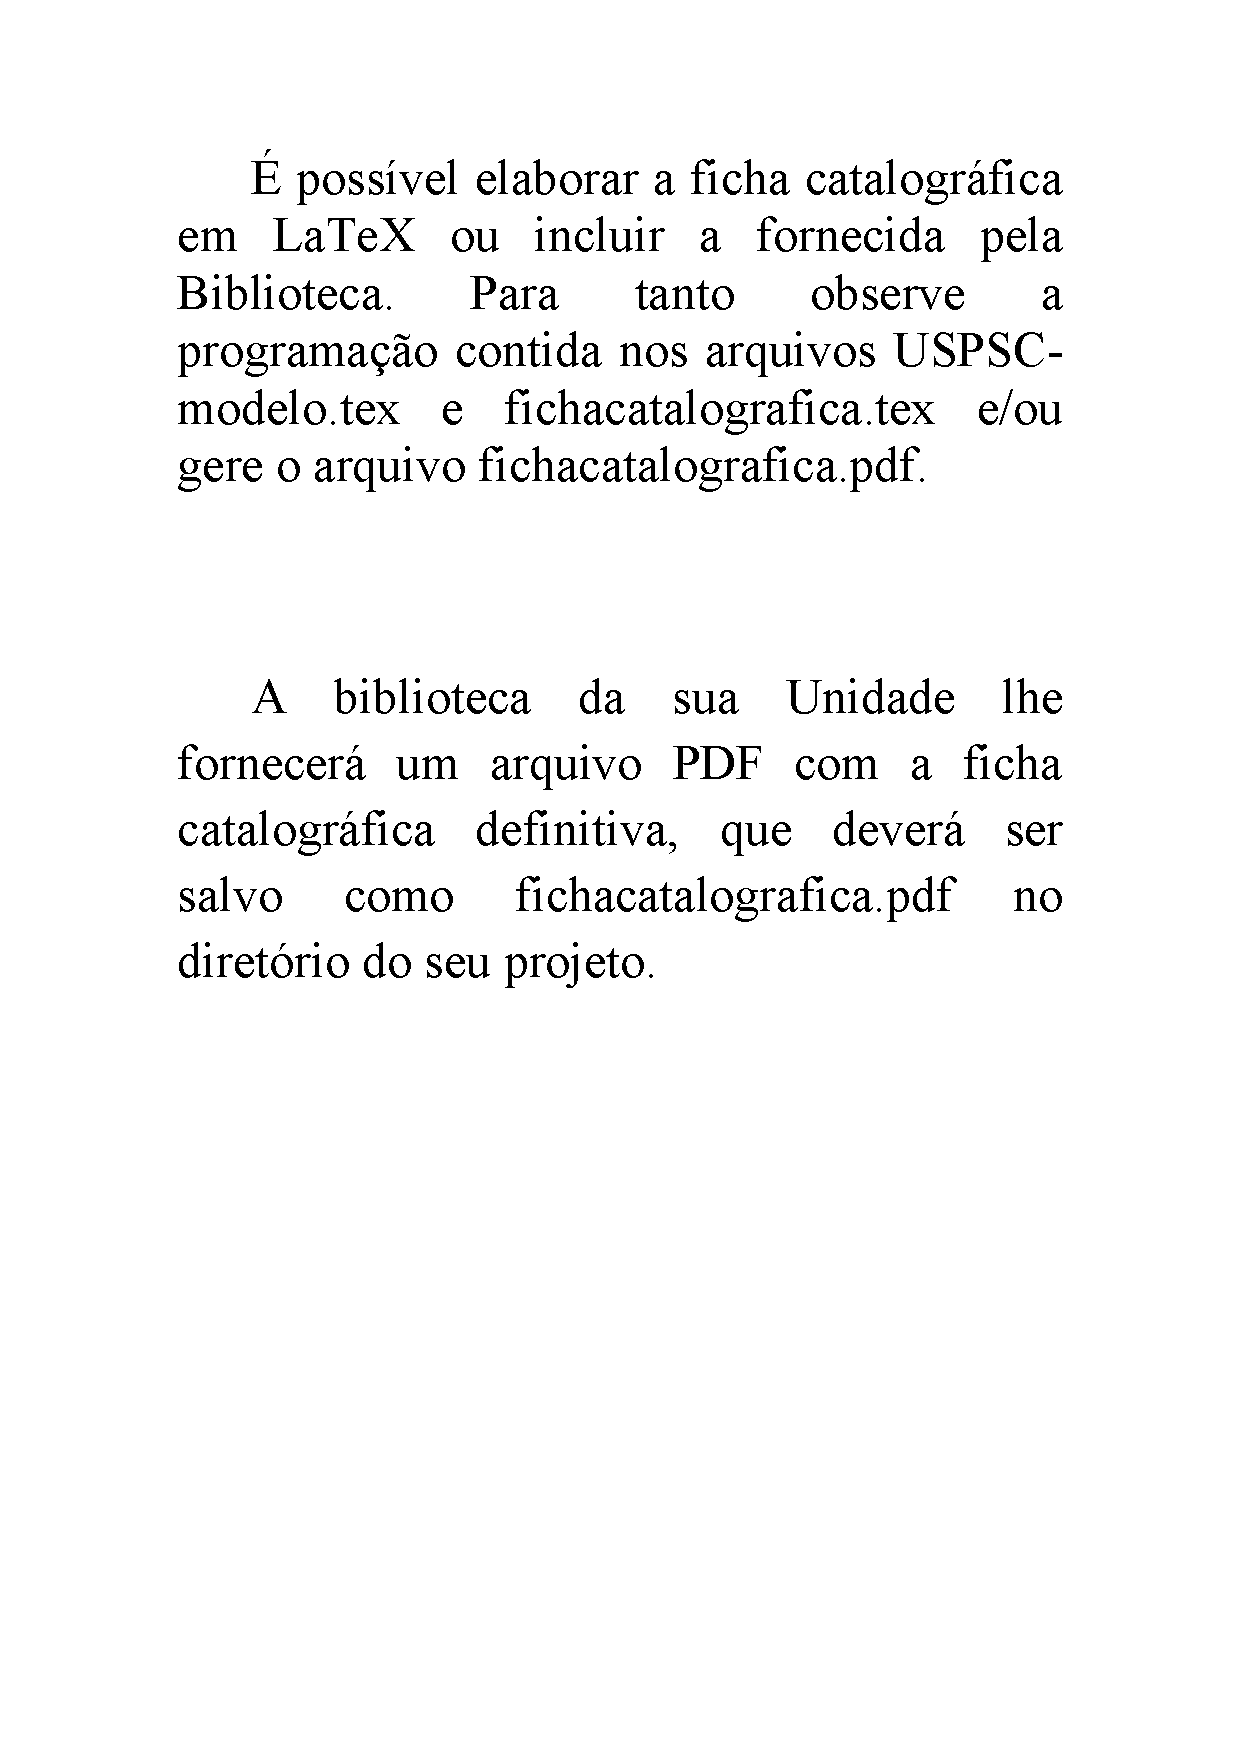
\includepdf{fichacatalografica.pdf} 
% Se você optar por elaborar a ficha catalográfica, deverá 
% incluir uma % antes da linha % antes
% do comando % ---
% Inserir a ficha bibliografica
% ---
% Isto é um exemplo de Ficha Catalográfica, ou ``Dados internacionais de
% catalogação-na-publicação''. Você pode utilizar este modelo como referência. 
% Porém, provavelmente a biblioteca da sua universidade lhe fornecerá um PDF
% com a ficha catalográfica definitiva após a defesa do trabalho. Quando estiver
% com o documento, salve-o como PDF no diretório do seu projeto e substitua todo
% o conteúdo de implementação deste arquivo pelo comando abaixo:
%
\begin{fichacatalografica}
	\hspace{-1.4cm}
	\imprimirnotaautorizacao \\ \\
	%\sffamily
	\vspace*{\fill}					% Posição vertical
	\begin{center}					% Minipage Centralizado
		\imprimirnotabib \\
\begin{table}[htb]
	\scriptsize
	\centering	
	\begin{tabular}{|p{0.9cm} p{8.7cm}|}
		\hline
	      & \\
		  &	  \imprimirautorficha     \\
		
		 \imprimircutter & 
							\hspace{0.4cm}\imprimirtitulo~  / ~\imprimirautor~ ;  ~\imprimirorientadorcorpoficha. -- 	\imprimirlocal, \imprimirdata.   \\
		
		  &  % Para incluir nota referente à versão corrigida no corpo da ficha,
			  % incluir % no início da linha acima e tirar a % do início da linha abaixo
			  %	\hspace{0.4cm} \imprimirtitulo~  / ~\imprimirautor~ ; ~\imprimirorientadorcorpoficha~- ~\imprimirnotafolharosto. -- \imprimirlocal, \imprimirdata.  \\
		
			\hspace{0.4cm}\pageref{LastPage} p. : il. (algumas color.) ; 30 cm.\\ 
		  & \\
		  & 
		    \hspace{0.4cm}\imprimirnotaficha ~--~ 
						  \imprimirunidademin, 
						  \imprimiruniversidademin, 
		                  \imprimirdata. \\ 
		  & \\                 
		   % Para incluir nota referente à versão corrigida em notas,
		    % incluir uma % no início da linha acima e	
		    % tirar a % do início da linha abaixo
		    % & \hspace{0.4cm}\imprimirnotafolharosto \\ 
		  & \\ 
		  & \hspace{0.4cm}1. LaTeX. 2. abnTeX. 3. Classe USPSC. 4. Editoração de texto. 5. Normalização da documentação. 6. Tese. 7. Dissertação. 8. Documentos (elaboração). 9. Documentos eletrônicos. I. \imprimirorientadorficha. 
		   II. Título. \\
	
		     %Se houver co-orientador, inclua % antes da linha (antes de II. Título.) 
		     %          e tire a % antes do comando abaixo 
		     %III. Título. \\   
		  \hline
	\end{tabular}
\end{table}
	\end{center}
\end{fichacatalografica}
% ---

 
% e retirar o % do comando abaixo
%% ---
% Inserir a ficha bibliografica
% ---
% Isto é um exemplo de Ficha Catalográfica, ou ``Dados internacionais de
% catalogação-na-publicação''. Você pode utilizar este modelo como referência. 
% Porém, provavelmente a biblioteca da sua universidade lhe fornecerá um PDF
% com a ficha catalográfica definitiva após a defesa do trabalho. Quando estiver
% com o documento, salve-o como PDF no diretório do seu projeto e substitua todo
% o conteúdo de implementação deste arquivo pelo comando abaixo:
%
\begin{fichacatalografica}
	\hspace{-1.4cm}
	\imprimirnotaautorizacao \\ \\
	%\sffamily
	\vspace*{\fill}					% Posição vertical
	\begin{center}					% Minipage Centralizado
		\imprimirnotabib \\
\begin{table}[htb]
	\scriptsize
	\centering	
	\begin{tabular}{|p{0.9cm} p{8.7cm}|}
		\hline
	      & \\
		  &	  \imprimirautorficha     \\
		
		 \imprimircutter & 
							\hspace{0.4cm}\imprimirtitulo~  / ~\imprimirautor~ ;  ~\imprimirorientadorcorpoficha. -- 	\imprimirlocal, \imprimirdata.   \\
		
		  &  % Para incluir nota referente à versão corrigida no corpo da ficha,
			  % incluir % no início da linha acima e tirar a % do início da linha abaixo
			  %	\hspace{0.4cm} \imprimirtitulo~  / ~\imprimirautor~ ; ~\imprimirorientadorcorpoficha~- ~\imprimirnotafolharosto. -- \imprimirlocal, \imprimirdata.  \\
		
			\hspace{0.4cm}\pageref{LastPage} p. : il. (algumas color.) ; 30 cm.\\ 
		  & \\
		  & 
		    \hspace{0.4cm}\imprimirnotaficha ~--~ 
						  \imprimirunidademin, 
						  \imprimiruniversidademin, 
		                  \imprimirdata. \\ 
		  & \\                 
		   % Para incluir nota referente à versão corrigida em notas,
		    % incluir uma % no início da linha acima e	
		    % tirar a % do início da linha abaixo
		    % & \hspace{0.4cm}\imprimirnotafolharosto \\ 
		  & \\ 
		  & \hspace{0.4cm}1. LaTeX. 2. abnTeX. 3. Classe USPSC. 4. Editoração de texto. 5. Normalização da documentação. 6. Tese. 7. Dissertação. 8. Documentos (elaboração). 9. Documentos eletrônicos. I. \imprimirorientadorficha. 
		   II. Título. \\
	
		     %Se houver co-orientador, inclua % antes da linha (antes de II. Título.) 
		     %          e tire a % antes do comando abaixo 
		     %III. Título. \\   
		  \hline
	\end{tabular}
\end{table}
	\end{center}
\end{fichacatalografica}
% ---


% As informações que compõem a ficha catalográfica estão 
% definidos no arquivo USPSC-pre-textual-UUUU.tex
% ---


% ---
% Inserir folha de aprovação
% ---
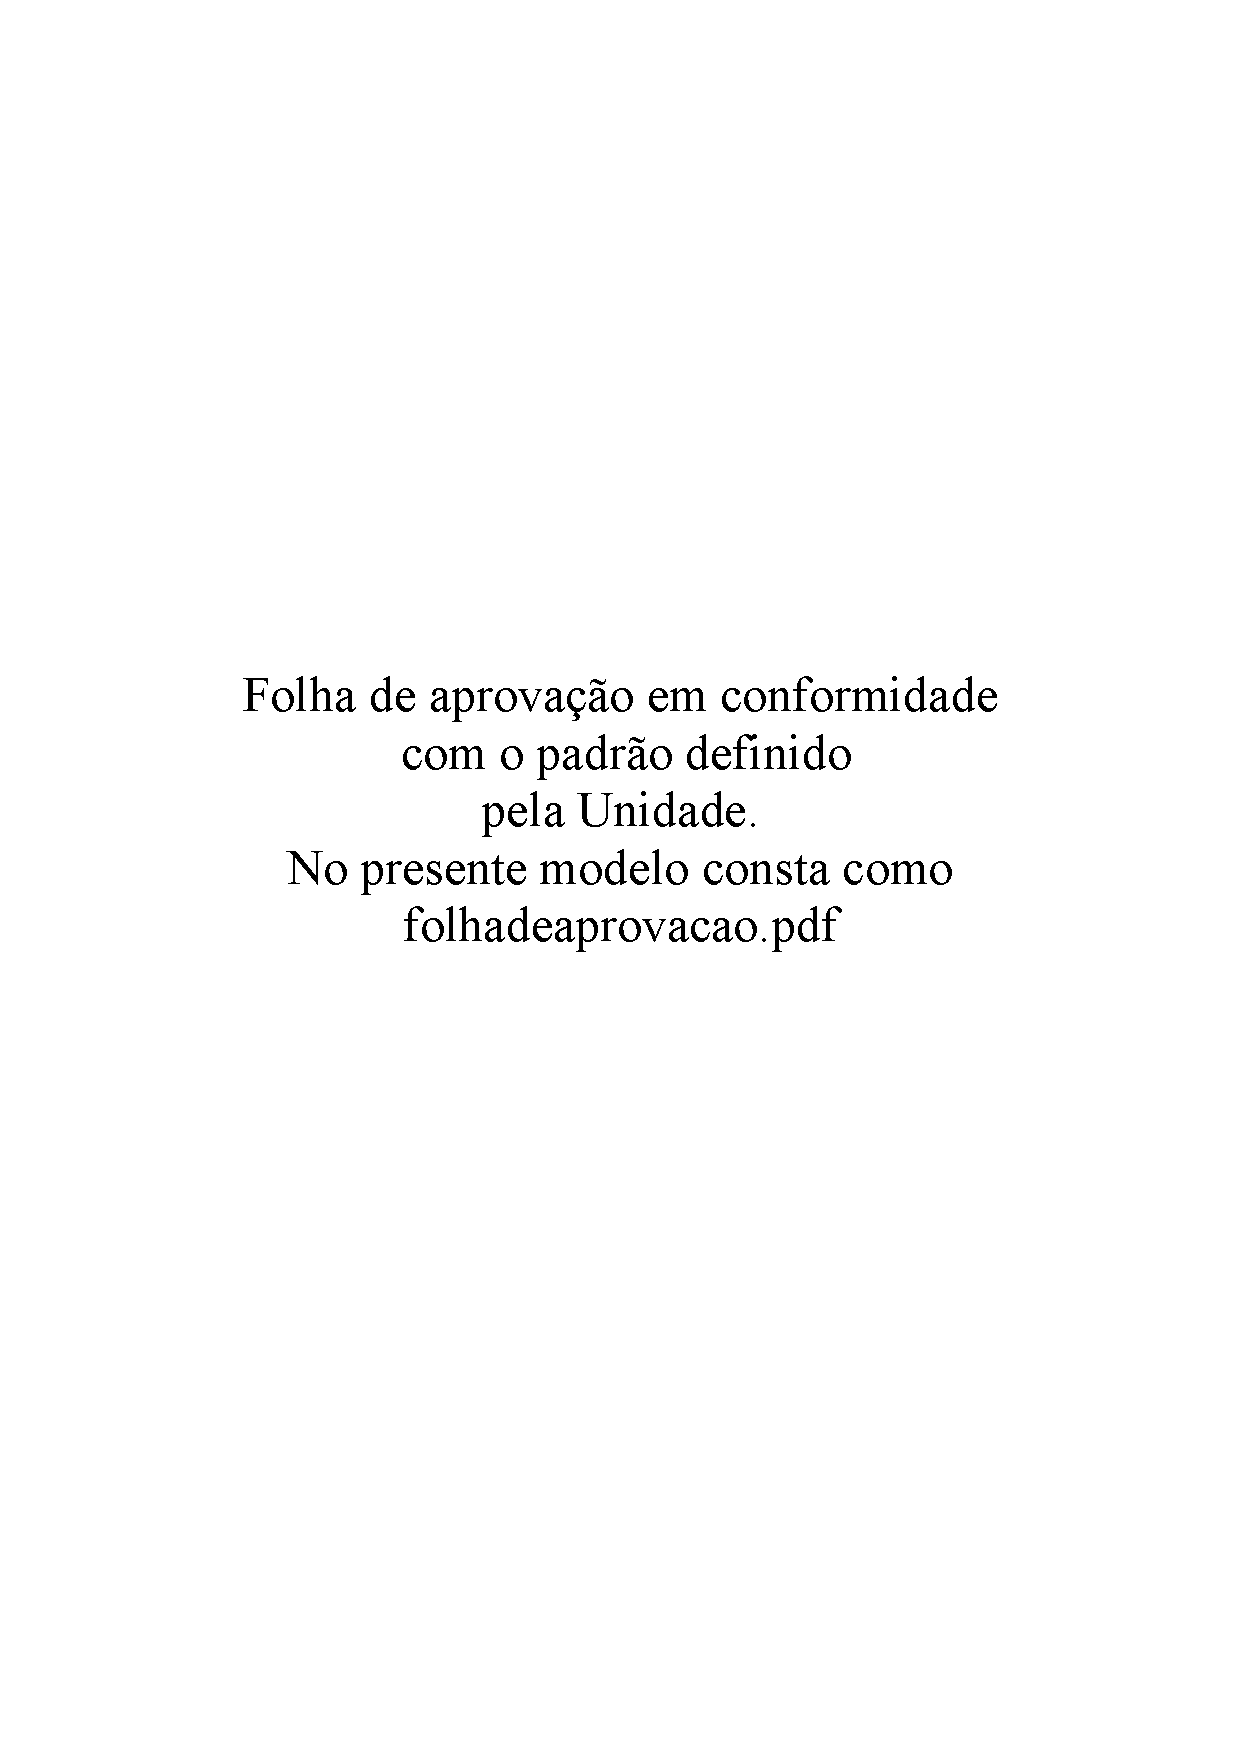
\includepdf{folhadeaprovacao.pdf}


\includepdf{PaginaEmBranco.pdf}

% ---
% Dedicatória
% ---
%%% USPSC-Dedicatória.tex                                                                                                
% ---                                                                                                                   
% Dedicatória                                                                                                           
% ---                                                                                                                   
\begin{dedicatoria}
   \vspace*{\fill}
   \centering
   \noindent
   \textit{To Vô Ernesto} \vspace*{\fill}
\end{dedicatoria}
% ---




% ---

% ---
% Agradecimentos
% ---
%% Agradecimentos.tex
% ---
% Agradecimentos
% ---=====
\begin{agradecimentos}
  I am very grateful to:
  \begin{itemize}
  \item
    %\item my advisor Prof. Vitor de Souza;

  %\item the LIP group, in particular to Prof. Mario Pimenta and Ruben Conceição; 

  %\item the KIT group, in particular to Michael Unger, Alex Herve and Darko Veberic; 
    
  %\item my collegues from the Astroparticle Physics group at IFSC;

  %\item family
    
  %\item friend
    
  %\item FAPESP
 
  \end{itemize}

\end{agradecimentos}
% ---

% ---

% ---
% Epígrafe
% ---
\begin{epigrafe}
    \vspace*{\fill}
	\begin{flushright}
		\textit{``Frogs are falling from the sky.''\\
		Albert Einstein}
	\end{flushright}
\end{epigrafe}
% ---

% A T E N Ç Ã O
% Se o idioma do texto for em inglês, o abstract deve preceder o resumo
% resumo em português
%
% Resumo
% ---
%% Abstract.tex
% ---
% Abstract
% ---
\autor{Prado, R. R.}
\begin{resumo}[Abstract]        
 \begin{otherlanguage*}{english}
	\begin{flushleft} 
		\setlength{\absparsep}{0pt} % ajusta o espaçamento dos parágrafos do resumo		
 		\SingleSpacing 
 		\imprimirautorabr~ ~\textbf{\imprimirtitleabstract}.	\imprimirdata.  \pageref{LastPage}p. 
		%Substitua p. por f. quando utilizar oneside em \documentclass
		%\pageref{LastPage}f.
		\imprimirtipotrabalho~-~\imprimirinstituicao, \imprimirlocal, 	\imprimirdata. 
 	\end{flushleft}
	\OnehalfSpacing 
   This is the english abstract.

   \vspace{\onelineskip}
 
   \noindent 
   \textbf{Keywords}: .
 \end{otherlanguage*}
\end{resumo}

% ---

% Abstract
% ---
%% Resumo.tex
% ---
% Resumo
% ---
\setlength{\absparsep}{18pt} % ajusta o espaçamento dos parágrafos do resumo		
\begin{resumo}[Resumo]
	\begin{flushleft} 
		        \setlength{\absparsep}{0pt} % ajusta o espaçamento da referência	
			\SingleSpacing 
			\imprimirautorabr~ ~\textbf{\imprimirtitleabstract}. \imprimirdata. \pageref{LastPage}p. 
			%Substitua p. por f. quando utilizar oneside em \documentclass
			%\pageref{LastPage}f.
			\imprimirtipotrabalho~-~\imprimirinstituicao, \imprimirlocal, \imprimirdata. 
 	\end{flushleft}
        \OnehalfSpacing 			

Raios C\'osmicos Ultra Energ\'eticos (Ultra-High Energy Cosmic Rays, UHECR) somente
podem ser medidos atrav\'es da detec\c{c}\~ao dos Chuveiros Atmosf\'ericos Extensos
(Extensive Air Showers, EAS) criados pela intera\c{c}\~ao do raio c\'osmico prim\'ario com
n\'ucleos atmof\'ericos. A infer\^encia de algumas propriedados dos UHECRs, como a composi\c{c}\~ao
de massa, \'e poss\'ivel somente atrav\'es da compara\c{c}\~ao entre medidas de observ\'aveis dos EASs
com predi\c{c}\~oes geradas por simula\c{c}\~oes de Monte Carlo. A fonte de incerteza mais importante
na descri\c{c}\~ao de EAS por simula\c{c}\~oes \'e a modelagem das intera\c{c}\~oes hadr\^onicas. Por muitos
anos \'e sabido que os modelos de intera\c{c}\~ao hadr\^onica falham na predi\c{c}\~ao de observ\'aveis
dos EASs relacionados a sua componente mu\^onica. A manifesta\c{c}\~ao mais evidente disso \'e 
chamada \emph{problema do d\'eficit de m\'uons} devido ao fato que o n\'umero de m\'uons em chuveiros
com energies acima de \E{18} predito por simula\c{c}\~oes \'e menor que os observados.
O objetivo desta tese \'e abordar este problema atrav\'es de tr\^es frentes. Primeiramente,
um m\'etodo \'e desenvolvido para interpretar as medidas do n\'umero de muons em termos
de composi\c{c}\~ao de raios c\'osmicos considerando o problema do d\'eficit de m\'uons.
Segundo, a proposta e o teste de um observ\'avel que \'e sens\'ivel ao espectro de energia dos m\'uons
na superf\'icie e, consequentemente, pode ser usado para constrair os modelos de intera\c{c}\~ao hadr\^onica.
Por \'ultima, a produ\c{c}\~ao de m\'uons em chuveiros \'e estudada atrav\'es
de medidas do espectro de produ\c{c}\~ao de hadrons em intera\c{c}\~oes do tipo p\'ion-carbono.



 \textbf{Palavras-chave}: Raios c\'osmicos de altas energies. Chuveiros atmsf\'ericos extensos. Componente mu\^onica de chuveiros atmosf\'ericos. F\'isica de chuveiros atmosf\'ericos.   
\end{resumo}

% ---

% ---
% inserir lista de figurass
% ---
\pdfbookmark[0]{\listfigurename}{lof}
\listoffigures*
\cleardoublepage
% ---

% ---
% inserir lista de tabelas
% ---
\pdfbookmark[0]{\listtablename}{lot}
\listoftables*
\cleardoublepage
% ---

% ---
% inserir lista de quadros
% ---
%\pdfbookmark[0]{\listofquadroname}{loq}
%\listofquadro*
%\cleardoublepage
% ---

% ---
% inserir lista de abreviaturas e siglas
% ---
%\begin{siglas}
%    \item[ABNT] Associação Brasileira de Normas Técnicas
%    \item[abnTeX] ABsurdas Normas para TeX
%	\item[EESC] Escola de Engenharia de São Carlos
%	\item[IAU] Instituto de Arquitetura e Urbanismo
%	\item[IBGE] Instituto Brasileiro de Geografia e Estatística
%	\item[ICMC] Instituto de Ciências Matemáticas e de Computação
%	\item[IFSC] Instituto de Física de São Carlos
%	\item[IQSC] Instituto de Química de São Carlos
%	\item[PDF] Portable Document Format
%	\item[TCC] Trabalho de Conclusão de Curso
%	\item[USP] Universidade de São Paulo
%	\item[USPSC] Campus USP de São Carlos
%\end{siglas}
% ---

% ---
% inserir lista de símbolos
% ---
%\begin{simbolos}
%  \item[$ \Gamma $] Letra grega Gama
%  \item[$ \Lambda $] Lambda
%  \item[$ \zeta $] Letra grega minúscula zeta
%  \item[$ \in $] Pertence
%\end{simbolos}
% ---
% ---
% inserir o sumario
% ---
\pdfbookmark[0]{\contentsname}{toc}
\tableofcontents*
\cleardoublepage
% ---
% ----------------------------------------------------------
% ELEMENTOS TEXTUAIS
% ----------------------------------------------------------
\textual

\chapter[Introduction]{Introduction}
\label{sec:introduction}

The Earth is constantly being reached by charged particles
coming from extraterrestrial sources, which are called Cosmic Rays.
For over a century, the study of these particles have been a very active field
that integrates aspects from both particle physics and astrophysics.
The extremelly wide energy range covered by the well know cosmic rays
energy spectrum make clear that a number of different astrophysical phenomena,
at distinct scales, are contributing to the production of these particles.

Of particular interest is the ultra-high energy range that includes
particles from $E=\E{17}$ up the end of the spectrum at $\sim\E{20.5}$. 
Althought the existence of these ultra-high energy particles is known
since the 1960's, due to detections done by Haverah Park experiment,
the precise measurements of their energy spectra and other features
became possible after the 1990's, with the experiments Fly's Eyes,
HiRes and AGASA. During the last decade, two modern experiments have
been running at the ultra-high energy range, Pierre Auger Observatory
and Telescope Array. 
Even though a large number of important results have been provided
by these experiments lately, the main question about the origin
of ultra-high energy cosmic rays are still unsolved. 
Apart from knowing the astrophysical sources and the acceleration
mechanisms, it is also unclear what is the exact nature of two evident structures
observed in the ultra-high energy spectrum, the \emph{ankle} and the \emph{suppression}.




Because of the very low flux of particles at the 



The compreesion of the astrophysical aspects behind the cosmic rays
is mainly complicated by the fact that they cannot be directly measured
at the high energy regime. Their detection is actually done by measuring
the cascade of particles created by the interaction of the cosmic ray particle
with atmospheric nuclei, the so called \emph{Extensive Air Showers}.  


Thus, the properties of the primary particles have to be infered from


The inferences of the properties of the primary cosmic ray have then
to be done by means of the measured features of the 





-cosmic rays->uhe->open questions

-cr->showers->understanding to infer

-muons->muon deficit problem

-augerprime->chap 3 and 4->simulation studies

-na61->pion-air








\chapter{Cosmic rays and the Pierre Auger Observatory}
\label{sec:uhecr}

In this chapter, an overview of cosmic rays physics will be given with focus 
on the ultra-high energy range, which is the range of interest of this thesis.
Recent reviews about the topic can be found in Refs.~\cite{Aloisio:2017ooo,Mollerach:2017idb}.
The Pierre Auger Observatory will also be introduced in~\cref{sec:uhecr:auger}.  


%%%%%%%%%%%%%%%%%%%%%%%%%%%%%%%%%%%%
\section{Overview of cosmic rays}
\label{sec:uhecr:overview}

%%================================%%
\subsection{Energy spectrum}

%%%%%%%%%%%%%% SPEC SWORDY %%%%%%%%%%%%%%%
\begin{figure}
  \centering
  
  \begin{overpic}[clip, rviewport=0 0 1 0.98,width=0.85\textwidth]{spectrum_swordy}
    \put(18,60){}
  \end{overpic}
  
  \caption{Compilation of measurements of the cosmic ray energy spectrum~\cite{SwordyPlot2001}.}
  \label{fig:uhecr:overview:spec:swordy}
\end{figure}

The cosmic ray flux as a function of energy is the so-called \emph{energy spectrum}
and it plays a central hole in the understanding of the astrophysical aspects behind these particles.
A compilation of measurements of the cosmic ray
energy spectrum over about 13 orders of magnitude
in energy is shown in~\cref{fig:uhecr:overview:spec:swordy}.
One can see that from \appE{11} up to the highest energies
the spectrum can be described approximately 
by a power law function, $\text{d}\phi/\text{d}E \sim E^{-\gamma}$, where
the spectral index $\gamma$ is not exactly constant over all the energy range
but it changes only slightly, between 2.5 and 3.2.
Because the cosmic ray spectrum extends over a very large
energy range, it is expected that different astrophysical mechanisms
at distinct length scales  
contribute to the production of these particles. An illustration
of that comes from the fact that most of the modern models predict that the
cosmic ray flux is dominated by particles produced inside our galaxy up to around \e{17}-\E{18} and,
above these energies, they have extragalactic origin. The transition between
these two components is currently one of the most active topics of discussion.

Because of the steepness of the spectrum, the particle flux changes over 27 orders of magnitude
from \e{11} to \E{21}. As indicated in~\cref{fig:uhecr:overview:spec:swordy},
while at \E{11} the flux is about one particle/m$^2$/second,
at \E{19} it drops to only one particle/km$^2$/year.
As a consequence, different experimental techniques have to be applied to detect
cosmic ray particles at different energy ranges. Up to \appE{14}, the high flux
allows us to use small area instruments installed in ballons or satellites
to detects the particles before they interact with the Earth's atmosphere.
Above this energy, the interaction with the atmosphere turns to be
useful since we can measure the cosmic rays indirectly through the detection of
the extensive air showers (see~\cref{sec:showers}). For that, large arrays of detectors
are used and their areas can vary substantially depending on the energy range they are
intended to be sensitive. As an example, the KASCADE experiment~\cite{\KASCADEPaper}
is designed to measure particles from around \e{14} to \E{16}
and it has an area of 4000 m$^2$, while Pierre Auger
Observatory~\cite{\AugerPaper} has an area of 3000 km$^2$ to measure particles above \E{18}.


A few features of the cosmic ray energy spectrum can be identified by the small changes on the
spectral index $\gamma$. To better visualize these changes, we show
in~\cref{fig:uhecr:overview:spec:pdg} a compilation of measurements of
the spectrum, starting at \appE{13}, in which the flux is scaled by a factor $E^{2.6}$.
As indicated in~\cref{fig:uhecr:overview:spec:pdg}, the lowest-energy feature
is the so-called \emph{first-knee} and it occurs around $3\times\E{15}$. At this energy
the index changes from $\gamma\approx 2.7$ to $3.0$. Increasing the energy, the next feature is
the so-called \emph{second-knee}, around \E{17}, where there is a further steepening
and the index goes to $\gamma\approx 3.3$. The spectrum then becomes harder again
at the \emph{ankle}, around $5\times\E{18}$, where the index changes to $\gamma\approx 2.6$.
The final feature occurs at the highest energies, above $4\E{19}$, where the
value of the spectral index becomes very high ($>4$), caracterizing the so-called
\emph{suppression}.


%%%%%%%%%%%%%% SPEC PDG %%%%%%%%%%%%%%%
\begin{figure}
  \centering
  
  \begin{overpic}[clip, rviewport=0 0 1 1,width=0.8\textwidth]{spectrum_pdg}
    \put(18,60){}
  \end{overpic}
  
  \caption{\cite{\PDGPaper}.}
  \label{fig:uhecr:overview:spec:pdg}
\end{figure}


The consistent interpretation of all these spectrum features requires the knowledge
about the composition of the cosmic rays. Particularly in the energy region compreending
the first and second-knee, very efficient composition measurements were performed
by KASCADE~\cite{\KASCADEPaper} and
KASCADE-Grande~\cite{\KASCADEGrandePaper} experiments. By using an experimental setup
that included surface detectors able to measured both number of charged particles and
number of muons in air showers, it was possible to measure the all particle spectrum
as well as to infer the spectra of individual groups of particles.
In~\cref{fig:uhecr:overview:spec:kascade}
we show the results of both experiments. Althought the final spectra are
strongly dependend on the hadronic interaction models
(see~\cref{sec:shower:simulations:models}) used in the analysis,
it is still possible to conclude that: (a) the first-knee is the result
of the suppression of the proton component of the spectrum~\cite{Antoni:2005wq},
(b) the suppression of the heavier components is consistent with
a rigidity dependent suppression~\cite{Antoni:2005wq} and (c) the second-knee coincides
with the suppression of the heaviest group of particles,
including iron nuclei~\cite{Apel:2011mi,Apel:2013uni}. 

%%%%%%%%%%%%%% SPEC KASCADE %%%%%%%%%%%%%%%
\begin{figure}
  \centering
  
  \begin{overpic}[clip, rviewport=0 0 1 1,width=0.8\textwidth]{kascade_spec}
    \put(18,60){}
  \end{overpic}

  \begin{overpic}[clip, rviewport=0 0 1 1,width=0.8\textwidth]{kascade_grande_spec}
    \put(18,60){}
  \end{overpic}
  
  \caption{\cite{Antoni:2005wq} \cite{Fuhrmann:2013lgx}.}
  \label{fig:uhecr:overview:spec:kascade}
\end{figure}


Although the rigidity dependent suppression as an explanation for the knee
was a known hypothesis since it was suggested by Peters, in 1961~\cite{Peters1961},
the actual explanation is still a matter of discussion. The most simple
model would assume that the suppression is a consequence of a limit
in the maximum energy reachable by the sources~\cite{Gaisser:2013bla}.  
Alternative models include explanations based on the effect of the
drifting of cosmic rays in the galactic magnetic field~\cite{Ptuskin1993,Candia:2002qd}
and on the escape of cosmic rays from the galaxy~\cite{Giacinti:2014xya}.
Most of the models, however, converge on the fact that up to the second-knee
the cosmic ray flux is dominated by a galactic component. The transition
between this galactic and an extra-galactic component would then occur
at energies around the second-knee and the ankle.
The measurements and the models concerning this energy range (above \E{17}),
the range of interest of this thesis,
will be presented in~\cref{sec:uhecr:spectrum}.


%%================================%%
\subsection{Acceleration and sources}

The power-law shape of the energy spectrum indicates that
cosmic rays are not accelerated in thermal processes.
A stochastic acceleration mechanism was first proposed
by Fermi, in 1949~\cite{Fermi:1949ee}. The main idea is that
the multiple collisions of charged particles with moving magnetized regions
could accelerate them up to high energies. 
Althought a power law spectrum can be derived from this mechanism,
the overall acceleration efficiency is too low to explain the observed
energy density of cosmic rays. The average energy gain is given by $\Delta E/E\sim \beta^2$,
where $\beta = v/c$ and $v$ is the velocity of magnetic cloud.
Because of this second power of $\beta$, this mechanism is
called \emph{second order Fermi mechanism}.

A similar but more efficient mechanism was developed almost
two decades later~\cite{Axford1977,Krymsky1977,Bell:1978zc,Blandford:1978ky}.
The main idea now is that charged particles collide with multiple shock waves
and they gain energy by interacting with irregularities in the magnetic field.
The average energy gain is $\Delta E/E\sim \beta$ and again the power law energy
spectrum can be derived. The obtained spectral index is $\gamma=2-2.3$, which means that
propagation effects have to be responsible to account for the further speepning
of the observed spectrum.
This mechanism is called \emph{first order Fermi mechanism} or, alternatively,
\emph{diffusive shock acceleration}, and it is the basis of most of the models
that propose possible sources of cosmic rays.
A detailed approach on the diffusive shock acceleration theory can be found
in Ref.~\cite{Drury:1983zz} and a review on alternative acceleration
models in Ref.\cite{}.

The list of astrophysical objects usually considered as possible
acceleraton sites for cosmic rays includes neutron stars~\cite{Fang:2012rx},
active galactic nuclei~\cite{}, gamma ray burst~\cite{Vietri1995,Waxman:2004ez}
and others. A review of the candidates
for sources of cosmic rays can be found in Ref.~\cite{Torres:2004hk}.
Indenpendently of the details about the acceleration mechanisms in different
types of astrophysical enviroments, it is possible to estimate the maximum energy
that a certain type of object is able to accelerate particles. This was first done
by Hillas~\cite{Hillas1984} and the idea is simply consider that
the Larmos radius of the particles must be smaller than the size of the site
in which the particles are confined to be accelerated. As a reults one obtain that
\begin{equation}
  \frac{E_\text{max}}{\E{18}} \approx \frac{\beta Z}{2} \frac{B}{\mu\text{G}}\frac{L}{\text{kpc}},
\end{equation}
where $\beta$ is the tipical velocity of the shock waves in units of $c$, $Z$ is the charge
of the particles, $B$ is the magnectic field and $L$ is the tipical size of the site.
The graphical illustration of this relation is usually called \emph{Hillas-plot}.
We show one version of it, focused on the candidate sources of ultra-high energy
cosmic rays, in~\cref{fig:uhecr:overview:hillas}.
The diagonal lines show the cases of \E{20} proton and iron nuclei.

%%%%%%%%%%%%%% HILLAS PLOT %%%%%%%%%%%%%%%
\begin{figure}
  \centering
  
  \begin{overpic}[clip, rviewport=0 0 1 1,width=0.8\textwidth]{hillas}
    \put(18,60){}
  \end{overpic}
  
  \caption{\cite{Mollerach:2017idb}}
  \label{fig:uhecr:overview:hillas}
\end{figure}


Regarding cosmic rays of ultra-high energy, a famous family of models,
generically called \emph{top-down models}, assume that
they are not accelerated by astrophysical objects, but intead they are the products
of the decay of exotic super-massive particles. The origin of these exotic particles
could be, for example, topological defects from early Universe phase transition
of even dark matter. As a prediction of nearly all these models, a significant flux of
ultra-high energy photons should be observed. However, measurements
of Pierre Auger Observatory have shown that the actual flux is much lower than
the predictions~\cite{Aglietta:2007yx} and, therefore, the top-down hypothesis can be ruled out.
A review on the top-down models can be found in Ref.\cite{Olinto2000}.  


%%================================%%
\subsection{Propagation of ultra-high energy cosmic rays}
\label{sec:uhecr:overview:propagation}


At the ultra-high energy regime, cosmic rays suffer from a number
of interaction processes during their propagation from the source to the Earth and
the consequent energy losses have a large influence on the measured
energy spectrum and composition.
Four interaction proccess take place: photopion production, electron pair production,
photodisintegration and adiabatic losses due to the expanse of the universe.
Since the latter affects equaly all types of particles with no dependence on
their energy, its influence on the energy spectra is the less relevant of all.
Concerning the other three remaining process,it is helpful to
evaluate their effect separetly for protons and nuclei.
In~\cref{fig:uhecr:propagation:attenuation} the protons energy losses are quantified by evaluating
the attenuation lenght, which is defined as the distance
over which the particle energy decreases by a factor $1/e$,
as a function of its energy.


%%%%%%%%%%%%%% ATTENUATION %%%%%%%%%%%%%%%
\begin{figure}
  \centering
  
  \begin{overpic}[clip, rviewport=0 0 1 1,width=0.8\textwidth]{att_lenght}
    \put(18,60){}
  \end{overpic}

 
  \caption{\cite{RafaelThesis}}
  \label{fig:uhecr:propagation:attenuation}
\end{figure}

The photopion production for protons, indicated by a blue curve in~\cref{fig:uhecr:propagation:attenuation},
occur because of the interaction of cosmic ray particle with photons
from the cosmic microwave background (CMB). The processes that take place are
$p+\gamma\rightarrow p + \pi^0$ and $p+\gamma\rightarrow n+ \pi^+$, in which
the energy threshold is given by the condition that the center-of-mass energy 
has to be larger than the rest mass of the pion. From~\cref{fig:uhecr:propagation:attenuation} it is clear
that photopion production losses dominate for energies above $\approx 8\times\E{19}$,
and, as a consequence, it is expected the proton spectrum to be strongly
suppressed around this energies.
This effect was proposed in 1966 by Greisen~\cite{Greisen:1966jv},
Zatsepin and Kuzmin~\cite{Zatsepin:1966jv}, and it is known as the GZK suppression.
It is also shown in~\cref{fig:uhecr:propagation:attenuation}
the energy losses due to electron pair production
during the proton propagation, which dominates at energies between $5\times\e{18}$ and
$5\times\E{19}$.

It can be seen that the combined effect of these two processes,
photopion production and electron pair production,
on the energy spectrum of cosmic rays composed purely by proton
can generate two evident features, a dip at $E\approx 5\times\E{18}$
and a sharp suppression above $E\approx 5\times\E{19}$, that
can explain the two features actually observed, the \emph{ankle}
and the \emph{suppression}~\cite{Berezinsky:2002nc,Berezinsky:2005cq}.
The pure proton composition predicted by this scenario has
two important consequencies. The first one is the so called
\emph{particle horizon}, meaning that protons above a certain energy
should be originated on average by sources inside a certain distance range.
In~\cref{fig:uhecr:propagation:horizon}
the particle horizon is quantified by curves that show the average energy
of protons as a fucntion of the propagation distance for three cases in which the
particle left the source with \e{20}, \e{21} and \E{22}. As a conclusion from this plot,
one can see that protons that reach Earth with $E>\E{20}$ are approximately limited to
be originated at sources within 100 Mpc of distance. The second consequence is related
to the particle deflections by magnectic fields. It is possible to show that
heavier nuclei are so strongly deflected that their arrival direction does not contain
informations about the direction of the astrophysical source. On the other hand,
since protons above $\approx\E{19}$ are only slightly deflected, in this pure-proton
scenario would be possible to use the arrival directions to infer the sources distribution.


%%%%%%%%%%%%%% GZK HORIZON %%%%%%%%%%%%%%%
\begin{figure}
  \centering
  
  \begin{overpic}[clip, rviewport=0 0 1 1,width=0.75\textwidth]{gzk_horizon}
    \put(18,60){}
  \end{overpic}
 
  \caption{\cite{Cronin:2004ye}}
  \label{fig:uhecr:propagation:horizon}
\end{figure}

Unlike protons, heavier nuclei also suffer photodisintegration along their propagation.
This means that they can interact with photons from the extragalactic background light (EBL)
and broke into smaller nuclei. In~\cref{fig:uhecr:propagation:attenuation} we show bla bla.
By comparing all the energy losses contribution for nuclei, one can see that
the energy threshold for photopion production and electron pair production
increases with the nuclei mass and the photodisintegration losses are the dominant ones.
The resultant effect of the propagation of a combination of different nuclei on the energy spectrum
turns to be more complicated to evaluate than in the proton case. However,
it is possible to show that, for example, in the simple case of pure iron nuclei being
originated at the sources, the energy spectrum would also suffer a suppression at the highest energies,
mainly due to photodissintegration effects. This suppression would be very similar to
the one expected because of the GZK effect and also to the one which is actually observed.
Concerning the other spectrum feature, the ankle, it is not possible to reproduce it
by considering nuclei propagation, instead of proton. The alternative explanation
for the ankle in the non-pure proton case is the effect of the
transition between galactic and extragalactic component. In~\cref{sec:uhecr:spectrum} we discuss
the recent measurements of the spectrum and composition at the ultra-high energies
and how they constrain the above mentioned explanation for the ankle and the suppression.



%%%%%%%%%%%%%%%%%%%%%%%%%%%%%%%%%%%%
\section{Energy spectrum and composition at ultra-high energies}
\label{sec:uhecr:spectrum}

At the ultra-high energy range, two very evident features can be observed
in the spectrum: the ankle and the suppression. In~\cref{fig:uhecr:spectrum}
we show the most up to date spectrum as measured
by Pierre Auger Observatory~\cite{AugerSpec2017} and Telescope Array~\cite{TASpec2017},
where both features can be clearly seen. The ankle is a hardening of the spectrum
at $E\approx 5\times \E{18}$ which was first observed
in Haverah Park measurements in 1963~\cite{LinsleySpec1963}, and later confirmed
in measurements by AGASA~\cite{AgasaSpecPaper1995}, HiRes~\cite{\HiResSpecPaper},
Pierre Auger Observatory~\cite{Abraham:2008ru}
and Telescope Array~\cite{}. The suppression is an abrupt softning of the flux
at energies above $4\times \E{19}$ which was measured first by Hires~\cite{\HiResSpecPaper}
and later confirmed by Pierre Auger Observatory~\cite{Abraham:2008ru} and Telescope Array~\cite{}.
The fact that the suppression was not observed on the AGASA spectrum~\cite{Takeda:1998ps}
was a source of intense discussions along years. However,
it is currently accepted that the AGASA measurements are not trustful because
of systematical errors in the primary energy estimation~\cite{}.

%%%%%%%%%%%%%% SPEC UHECR %%%%%%%%%%%%%%%
\begin{figure}
  \centering
  
  \begin{overpic}[clip, rviewport=0 0 1 1,width=0.8\textwidth]{uhecr_spectrum}
    \put(18,60){}
  \end{overpic}
  
  \caption{\cite{AugerSpec2017,TASpec2017}.}
  \label{fig:uhecr:spectrum}
\end{figure}


The most precise inferences of the composition of cosmic rays
at this energy range are based on the \xmax measurements
performed by fluorescence telescopes in the modern experiments.
In~\cref{sec:shower:observables}, we present a detailed discussion about
the \xmax measurements, its composition interpretation, as well as
further measurements of air shower observables that could, in principle,
be used to infer composition. For now, it is only important to
point out that the cosmic rays composition
can be infered by comparing the measured \xmax distributions to
predictions obtained from air shower simulations. This procedure can be done
either by comparing only the moments of the \xmax distributions, which
gives only the average composition, or by comparing the whole distributions,
which can provide the abundances of individual groups of primaries.
In all cases, the composition interpretation is dependent on the
hadronic interaction model used to generate the simulation predictions.

Althought the energy spectrum with its both features can be sucesfully described
by multiple hypothesis, the composition measurements must be used to further constrain  
the models. Concerning the ankle, most of the models associate it to
the transition between the galactic and extra-galactic flux, which
can take place in energies between the second-knee and the ankle.
The composition predictions by these models can vary substantially depending
on the exact position of the transition and on the composition content of
the extra-galactic component. One historically relevant hypothesis to
describe the ankle without the galactic-to-extragalactic transition assumption is the
so called \emph{dip model}~\cite{Berezinsky:2002nc,Berezinsky:2005cq},
which proposes that the energy losses due to
pair production along the particle propagation would cause the hardening
of the spectrum around the ankle energies. It turns out that the success
of the dip model actually requires a nearly pure proton composition
around and above the ankle. Althought at the time of the model proposal
this composition assumption seemed to be fulfilled by the \xmax measurements
of HiRes experiments~\cite{\HiResXmaxPaper},
recent measurements of Pierre Auger Observatory
have proven it wrong~\cite{\AugerXmaxPRLPaper}.

Concerning the suppression, the two currently consided hypothesis
to explain it are the GZK effect (see~\cref{sec:uhecr:overview:propagation})
and the limit of the acceleration power by the sources. While the GZK hypothesis
require a composition dominated by protons at the highest energies, the source limit
would imply in a rigidity dependent suppression and consequently a increasingly heavier
composition as the energy increase. Similarly to what happened to the dip model,
the composition measurements by HiRes supported the GZK hypothesis for many year,
which was also changed after the Pierre Auger Observatory published its \xmax measurements
results. 

Many scenarios which propose to explain the ultra-high energy spectrum and composition
can be found in the
literature~\cite{Allard:2005cx,Aloisio:2011fv,Biermann:2011wf,Unger:2015laa,Globus:2015xga}.
Two features are commom to nearly all the recent models that are contrained by the
Auger \xmax measurements: the exact energy of the galactic-extragactic transition
(the energy in which both flux become equivalent) is around $1-4 \times \E{18}$
and the suppression is caused by a riditity dependent cutoff due to the limit
of the acceleration power of the sources. 
The absence of the GZK effect and its negative consequences
(e.g. the absence of correlation with nearby sources due to the deflection of
heavy nuclei in magnetic fields) have motivated the author of Ref.~\cite{Aloisio:2011fv}
to call this generic scenario of \emph{disappointing model}.

In a recent analysis done by Pierre Auger Collaboration,
the measured spectrum and the \xmax distributions were
jointly fitted by using simulations which account for
all the propagation effects~\cite{Aab:2016zth}.
We show in~\cref{fig:uhecr:combined} the results
of the fit by using the hadronic interaction model \EposLHCLong~\cite{\EposLHCPaper}
to simulate the \xmax distributions. The hypothesis of the limit of the acceleration power
by the sources as the source of the suppression is confirmed by the results of this analysis.
However, the lack of information about the composition given by the \xmax measurements
at energies above $4\times\E{19}$ is a limiting factor for this analysis, since the
spectrum is measured up to above \E{20}. Therefore, precise composition measurements
at the highest energies is a requirement to refine the interpretation
of the end of the cosmic rays spectrum. 

%%%%%%%%%%%%%% COMBINED FIT %%%%%%%%%%%%%%%
\begin{figure}
  \centering
  
  \begin{overpic}[clip, rviewport=0 0 1 1,width=0.9\textwidth]{combined_fit}
    \put(18,60){}
  \end{overpic}
  
  \caption{\cite{Aab:2016zth}.}
  \label{fig:uhecr:combined}
\end{figure}




%%%%%%%%%%%%%%%%%%%%%%%%%%%%%%%%%%%%
\section{The Pierre Auger Observatory}
\label{sec:uhecr:auger}

The Pierre Auger Observatory was designed to measure
cosmic rays at the ultra-high energy range.
It is located near the town of Malargue, Argentina,
and its total area is approximately 3000 km$^2$.
The average altitude of the experiment is 1420 m, which
corresponds to a vertival atmospheric depth of approximately 880 g/cm$^2$.
The construct of the observatory started in 2002 and completed in 2008.
Its hybrid detection system, which combines a large surface detector 
and a set of fluorescence telescopes, is one of the most important experimental features
of the Pierre Auger Observatory. A detailed overview of the experiment
can be found in Ref.~\cite{\AugerPaper}.

%%%%%%%%%%%%%% AUGER ARRAY %%%%%%%%%%%%%%%
\begin{figure}
  \centering
  
  \begin{overpic}[clip, rviewport=0 0 1 1,width=0.6\textwidth]{auger_array}
    \put(18,60){}
  \end{overpic}
  
  \caption{}
  \label{fig:uhecr:auger:array}
\end{figure}


The standard surface detector (SD) is composed by a set of $\sim 1660$
water-Cherenkov detectors (WCD) which are regularly arranged in a triangular grid.
The nearest neighbor distance of the stations for the standard array,
which covers the full observatory area, is 1.5 km, while a small area of YYY km$^2$
called \emph{SD infill} contains stations separated by 750 m.
In~\cref{fig:uhecr:auger:array} the stations of the SD array
are shown as black dots. Each WCD consists of a cylindrical tank with a diameter of 3.6 m,
filled with 12 m$^3$ of ultra-high purity water, up to a height of 1.2 m. The particle
detection is done by collecting the Cherenkov light produced by the passage of charged
particle throught the water. For that, three photomultiplier tube (PMT) are installed
on the top of each station and their signal are extracted and digitalised using FADCs
with a sampling rate of 40 MHz. Since the SD operation does not
require any special enviromental condition, its duty cicle turns to be very
close to 100\%.
More details about the SD can be found in Ref.\cite{Allekotte:2007sf}.


The fluorescence detector (FD) is composed by 27 telescopes installed in
4 buildings around the edge of the array. Each of these buildings contains
a set of six telescopes with a field of view which covers \dg{30} horizontally
and goes from \dg{1.5} to \dg{30} vertically. The 24 telescopes of this kind
were part of the original project of the observatory and they are designed to measure
the fluorescence light emitted by the atmosphere during the development of air showers
with primary energies above approximately \E{18}. Another set of 3 telescopes
that can operate with a vertical field of view going from \dg{30} to \dg{60}
was later installed in one the buildings.
This enhancement is called HEAT~\cite{Mathes:2011zz} and it is
designed to extend the lower limit of the fluorescence measurements to approximately \E{17}.
In~\cref{fig:uhecr:auger:array}
blue and red lines are used to show the field of view of the standard telescopes
and the HEAT ones, respectivelly. Because of its sensitivity, the background light has to be avoided
during the FD operation. This means that moonless nights with proper atmospheric conditions
are required, implying in a duty cicle of about 13\% for the FD measurements. 
More details about the FD can be found in Ref.\cite{Abraham:2009pm}.

The SD and FD measurements provide complementary informations 
which can be combined to achieve a precise reconstruction of the
properties of the air shower and the primary particle.
However, because of the limited FD duty cicle, both informations
are only available to a fraction of the events. Because of that,
two different event reconstruction modes are defined, the SD and
the hybrid reconstruction.

The hybrid reconstruction uses the measurements of the
fluorescence telescopes with only additional timing information
from one SD station. From the time structure of the FD signal it is
possible to reconstruct precisely the geometry of the shower and
from the amount of light collected it is possible to reconstruct the
longitudinal profile of the shower. A detailed procedure has to be applied
at this point to convert the number of photons colected into energy deposit
in the atmosphere by taking into account the atmospheric attenutation.
One example of longitudinal profile as measured by Auger is shown
on the right plot of~\cref{fig:uhecr:auger:rec}.
After obtained the energy deposit as a function of slanth depth,
a Gaisser-Hillas function~\cite{GaisserHillas1977} is fitted to that and the result
is used to determine the shower maximum \xmax and the calorimetric energy,
which is given by the integral of the fitted function. This calorimetric
energy is then corrected by the invisible energy due to neutrinos and high energy
muons and the final FD energy ($E_\text{FD}$) is then obtained.

%%%%%%%%%%%%%% AUGER REC %%%%%%%%%%%%%%%
\begin{figure}
  \centering
  
  \begin{overpic}[clip, rviewport=0 0 1 1,width=0.45\textwidth]{auger_long_profile}
    \put(18,60){}
  \end{overpic}
  \begin{overpic}[clip, rviewport=0 0 1 1,width=0.45\textwidth]{auger_lat_dist}
    \put(18,60){}
  \end{overpic}
  
  \caption{\cite{\AugerXmaxPRDPaper} \cite{\AugerPaper}}
  \label{fig:uhecr:auger:rec}
\end{figure}


The SD reconstruction is based on the size and the times of signals registered
by the individual stations. The geometry of the shower is first determined
by fitting the time of the signals assuming a spherical shape for the shower front.
After obtaining the shower geometry it is possible to evaluate the lateral distribution,
which is basically the evolution of the station signals with the distance to the
shower axis. On the left plot of~\cref{fig:uhecr:auger:rec}
we show one example of the lateral distribution function
as measured by Auger. A function of the NKG type~\cite{Kamata1958,Greisen1956} is fitted
and the evaluation of fitted function at a certain distance is defined
as shower size. For the standard array, with stations at 1500 m distance from each other,
the signal is evaluated at 1000 m and the shower size is represented by $S(1000)$.
The determination of the energy of SD reconstructed showers is done
by means of an energy calibration procedure, in which a set of hybrid reconstructed
showers are used to relate the shower size estimated from SD to the calorimetric
energy estimated by FD.


The first step of the energy calibration is to correct the $S(1000)$ parameter
for the atmospheric attenutaion effects. This is done by following the
Constant Instant Cut (CIC) method~\cite{CIC1961} which, by assuming that the flux
of cosmic rays above a certain energy is isotropic, correct the zenith angle dependence
of $S(1000)$ by converting it to a certain reference zenith angle. For the standard array,
this reference value is \dg{38} and the corrected shower size is represented by $S_{38}$.
The next step is selecting a sample of high quality hybrid events and use them
to relate the $S_{38}$ and $E_\text{FD}$. This relation is parametrized by a power law function
of the type $E_\text{FD} = A (S_{38})^B$ which is fitted to the data.
In~\cref{fig:uhecr:auger:cal} we show one example of the $S_{38}$ vs $E_\text{FD}$ plot with the fitted
function. The parameters resulting from the fit are used to determine
the SD energy from the $S_{38}$ parameter. 

%%%%%%%%%%%%%% AUGER CAL %%%%%%%%%%%%%%%
\begin{wrapfigure}{r}{0.55\textwidth}
  \centering
  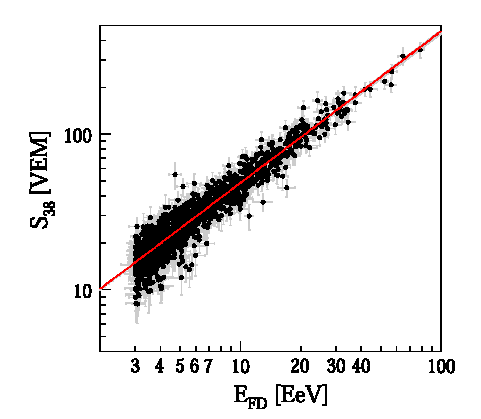
\includegraphics[width=0.55\textwidth]{auger_calibration}
  \caption{\cite{\AugerPaper}}
  \label{fig:uhecr:auger:cal}
\end{wrapfigure}


More details about the standard event reconstruction
can be found in Ref.~\cite{\AugerPaper}. Besides the SD and hybrid
reconstruction, a spectial procedure is applied to highly inclined
air showers, with zenith angle larger than \dg{60}. Th details about
this reconstruction can be found in Ref.\cite{Aab:2014gua}.

Apart from the SD and FD, a number of other detectors are currently
part of the Pierre Auger Observatory.
The muon detector called AMIGA~\cite{Suarez:2013ecb,Wundheiler:2011zz,Platino:2011zz}
(Auger Muons and Infill for the Ground Array) and the radio detector
called AERA (Auger Engineering Radio Array)~\cite{Kelley:2011zz} are already installed
and operating. Moreover, prototypes of a recently developed muon detector
named MARTA~\cite{Abreu:2017vsj} will be installed in the near future.


%%================================%%
\subsection{AugerPrime}

An example of the importance of the Auger spectrum
and mass composition measurements at the highest energies was
already given in~\cref{sec:uhecr:spectrum},
where the results of the combined fit were discussed~\cite{Aab:2016zth}. 
Besides that, further recent analysis by Auger have provided very
important results concerning the astrophysical origins of
the ultra-high energy cosmic rays. Two of these results
are worthwhile mentioning: a large scale dipolar anisotropy
of $\sim 6\%$ found for energies above $8\times \E{18}$~\cite{Aab:2017tyv}
and evidences of anisotropy in the arrival directions
of cosmic rays with $E>E{19}$ which indicates correlation with
nearby extragalactic sources~\cite{Aab:2018chp}. Even though these recents results
represent a great progress on the understanding of the nature and origin
of the highest energies cosmic rays, the main questions remain still
open.

An important piece of information to be provided experimentally that
is still missing is the mass composition of cosmic rays above $3 \times \E{19}$.
Althought the composition can be infered trustfully from \xmax measurements
(see~\cref{sec:shower:observables:xmax}),
the low duty cicle of the fluorescence telescopes prevents
it to be used above the suppression energy.
Overcoming this issue is the main goal of the upgrade of the Pierre Auger Observatory,
called AugerPrime~\cite{Aab:2016vlz,Martello:2017pch}.
Besides elucidating the mass composition at the highest energies,
the goals of AugerPrime also include searching for a flux contribution of protons up to the highest
energies and studying the properties of air showers and hadronic multiparticle production.
The latter one is intrinsically related
to the muon deficit problem (see~\cref{sec:shower:observables:nmu}),
which is the main topic of this thesis.

The experimental configuration of AugerPrime consists of four components.
The first one is the Surface Detector Electronics Upgrade (SDEU), intending to provide
a large number of improvements to the SD electronics, which includes the increasing of
analog-to-digital converter sampling rate from 40 MHz to 120 MHz~\cite{Suomijarvi:2017ixb}.
The second component is the changing
on the FD operation mode intending to increase its duty cycle up to 20\%.
The remaining two components are related to the detection of muons with surface detectors and
they are the Scintilattors Surface Detectors (SSD) and
Underground Muon Detectors (UMD).

The SSD consists of scientilattor detectors installed on the top of each existing WCD.
Since the scintilattors and water-Cherenkov tanks respond differently to the muonic and
electromagnetic component of the shower, the combination of both measurements
can be used to estimate the muon content~\cite{Gonzalez:2016ora}. 
The UMD consists of scintilattors buried 1.3 m below the ground, near the SD stations,
which are able to detect muons isolatelly with an energy threshold around 1 \GeV. The design
of the UMD will follow the same as the AMIGA detector~\cite{Suarez:2013ecb,Wundheiler:2011zz,Platino:2011zz}
that has already been developed during the last years. While the SSD will cover the full
standard array, with over 1600 stations, the UMD will be installed on the smaller area
of the SD infill.

The precise measurements of the muonic component is surely one of the most relevant
result to be provided by AugerPrime. As a consequence it is expected a signicant
improvement on the current understanding of the air shower physics, and in particular
the muon production. Both analysis presented in~\cref{sec:interpretation,sec:observable}
consider muon detectors similar to the ones of AugerPrime.




\chapter[Extensive air showers]{Extensive air showers}
\label{sec:showers}


\section{Particle production}


\section{Observables}





\chapter[Interpretation of measurements of the number of muons in extensive air shower experiments]{Interpretation of measurements of the number of muons in extensive air shower experiments}
\label{sec:interpretation}

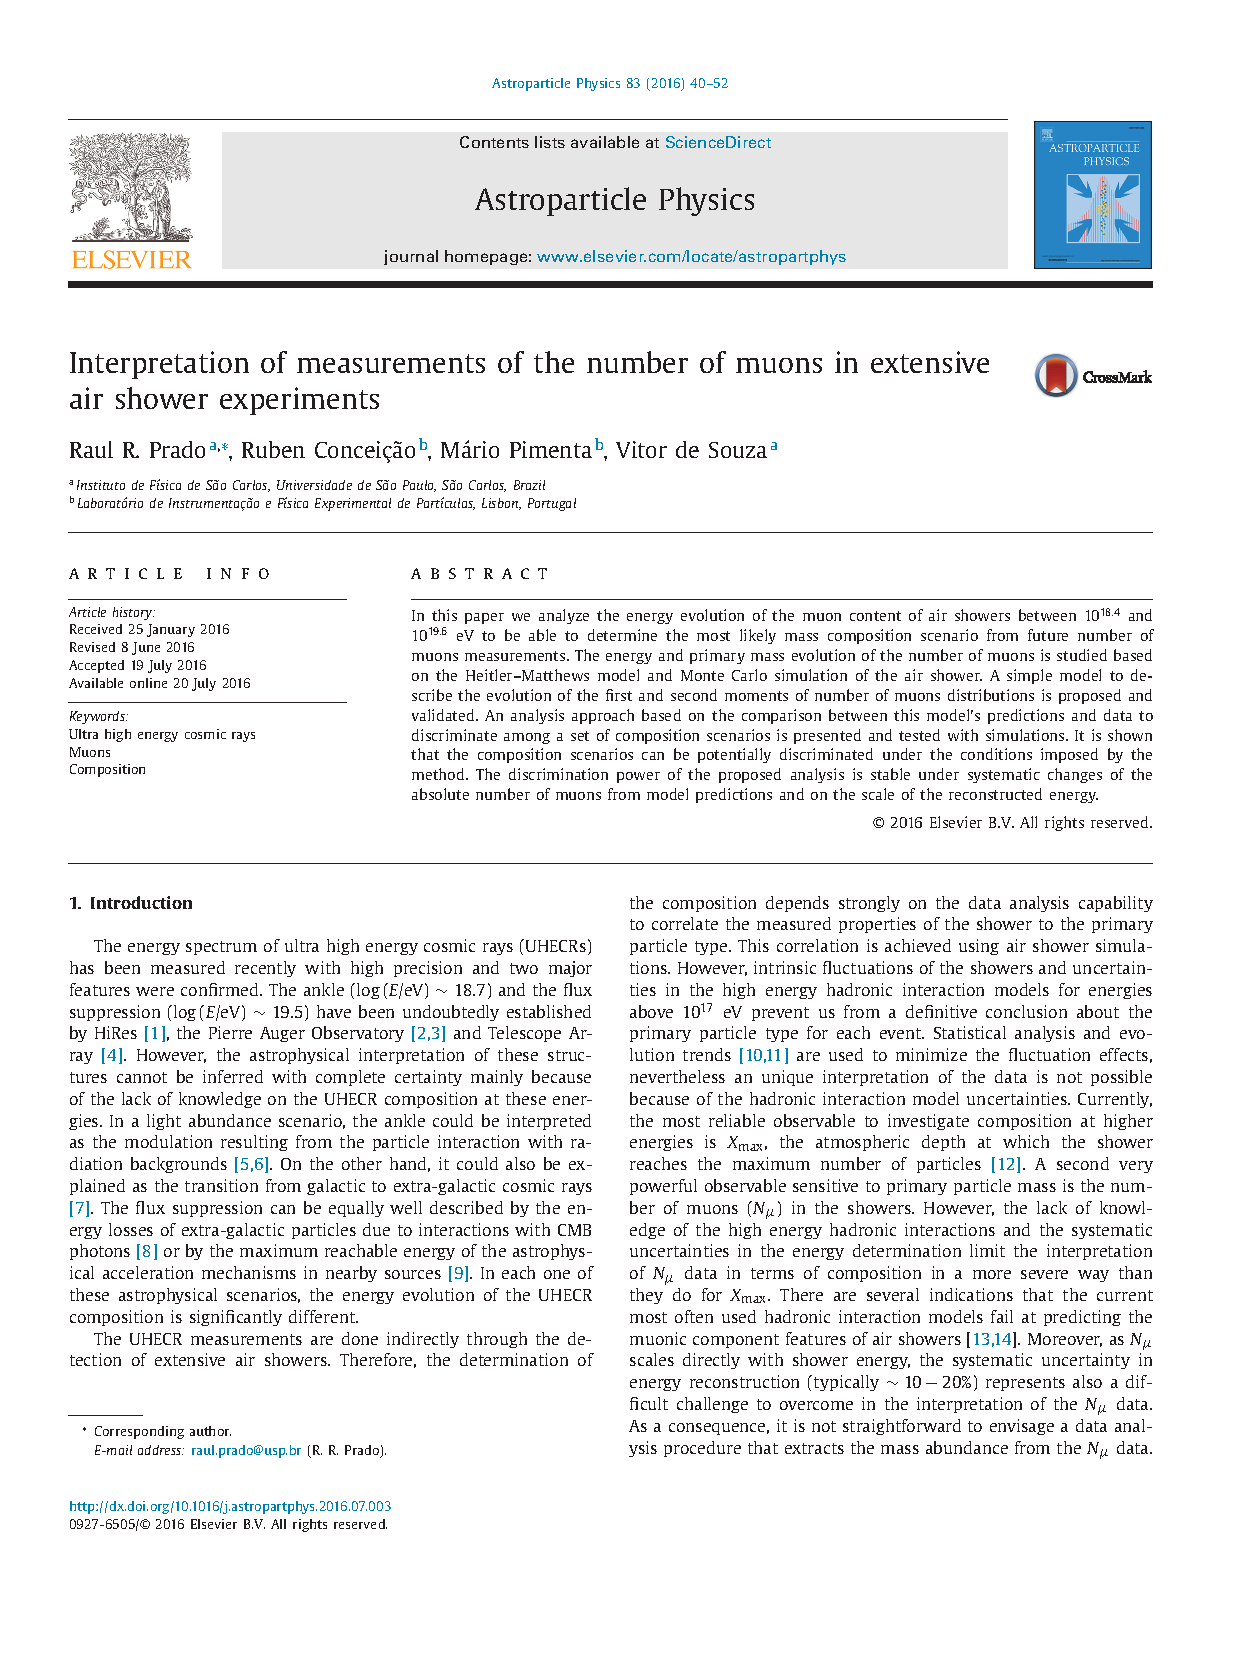
\includepdf[pages=-]{paper_interpretation.pdf}




\chapter[A new air-shower observable to constrain hadronic interaction models]{A new air-shower observable to constrain hadronic interaction models}
\label{sec:observable}

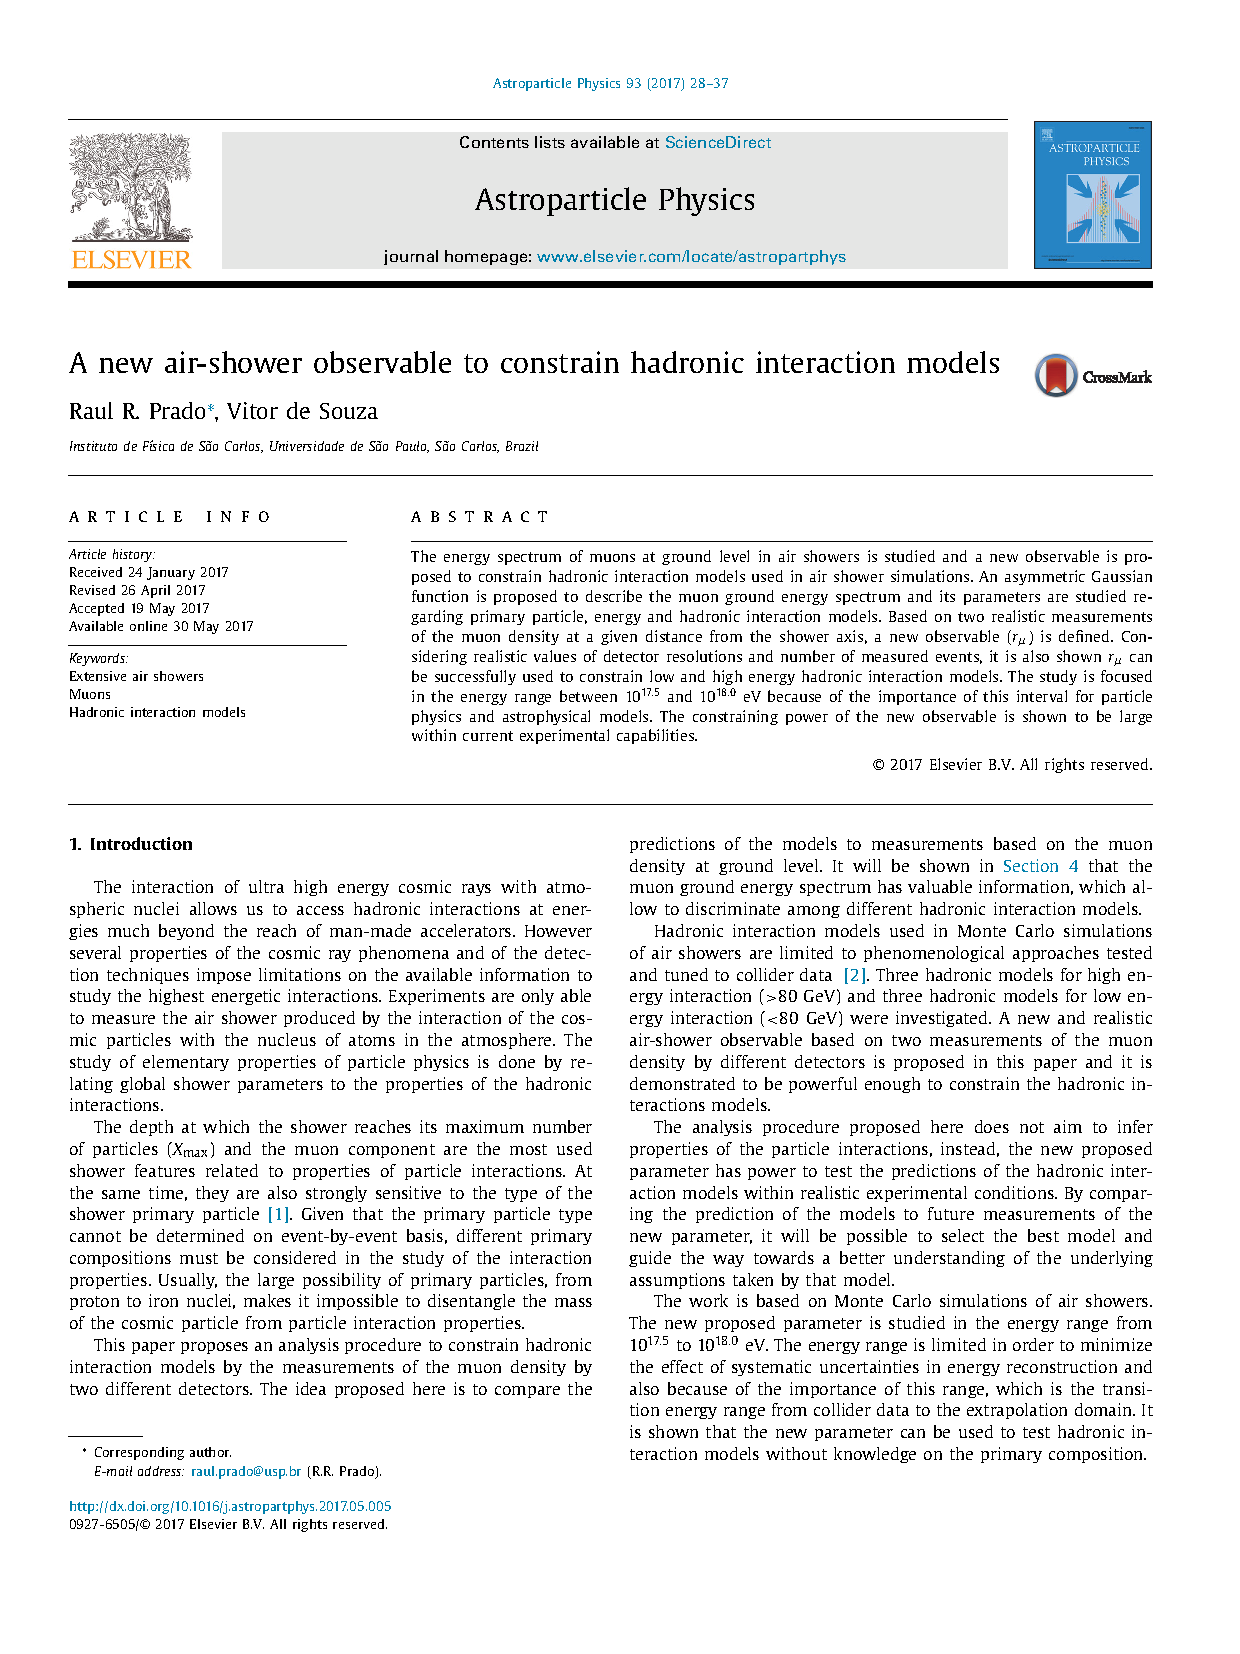
\includepdf[pages=-, pagecommand={}]{paper_observable.pdf}



\chapter[Hadron production in pion-carbon interactions]{Hadron production in pion-carbon interactions}
\label{sec:hadron}


\cite{\NASixtyOnePaper}

\cite{\NAFortyNinePaper}

\cite{\RhoPaper}

\cite{\ICRC17}

%\cite{\APP17}

%\cite{\APP16}

\cite{\QGSJetPaper}

\cite{\DPMJetPaper}

\cite{\EposPaper}



%\clearpage

%%%%%%%%%%% DIST %%%%%%%%%%%%%%%%%%
\begin{figure}
  \centering

  \begin{overpic}[clip, rviewport=0 0 1 1,width=0.4\textwidth]{dedx/dist_350_v0_c0_x13_y3}
    \put(16,85){(a)}
  \end{overpic}
  \begin{overpic}[clip, rviewport=0 0 1 1,width=0.4\textwidth]{dedx/dist_350_v0_c1_x13_y3}
    \put(16,85){(b)}
  \end{overpic}

  \vspace{0.5cm}
  
  \begin{overpic}[clip, rviewport=0 0 1 1,width=0.4\textwidth]{dedx/dist_350_v1_c0_x29_y5}
    \put(16,85){(c)}
  \end{overpic}
  \begin{overpic}[clip, rviewport=0 0 1 1,width=0.4\textwidth]{dedx/dist_350_v1_c1_x29_y5}
    \put(16,85){(d)}
  \end{overpic}
  
  \caption{Examples of the fitted \dedx distributions from the 350 \GeVc dataset.
    On the top, the distributions of the (a) negatively and (b) positively charged
    tracks are shown for one phase space bin of the RST subset. On the bottom,
    the distributions of the (c) negatively and (d) positively charged
    tracks are shown for a different phase space bin of the WST subset.
    The values of the $\langle\pp\rangle$ and $\langle\pT\rangle$ for
    each phase space bin is indicated on the top of each plot.
    The black dots show the observed number of tracks, while the colored
    distributions are the results of the \dedx fit or each particle type. 
    On the bottom of each plot, we show the residual of the fit, defined
    as the difference between the observed and the expected number of tracks
    from the result of the fit, divided by the uncertainty of the observed number.}
  \label{fig:hadron:dedx:fit:dist350}
\end{figure}



%%%%%%%%%% CHI SQ %%%%%%%%%%%%%%
\begin{figure}
  \centering

  \begin{overpic}[clip, rviewport=0 0 1 0.945,width=0.4\textwidth]{dedx/chisq_350_v0}
    \put(18,58){(a)}
  \end{overpic}
  \begin{overpic}[clip, rviewport=0 0 1 0.945,width=0.4\textwidth]{dedx/chisq_350_v0}
    \put(18,58){(b)}
  \end{overpic}

  \caption{\redchisq of the \dedx fit for the 350 \GeVc data set.
    The RST and WST are shown in (a) and (b), respectively.}
  \label{fig:hadron:dedx:fit:chi350}
\end{figure}

%%%%%%%%%% CAL %%%%%%%%%%%%%%
\begin{figure}[!ht]
  \centering

  \begin{overpic}[clip, rviewport=0 0 1 0.94,width=0.49\textwidth]{dedx/model_158_v1_m0}
    \put(18,58){(a)}
  \end{overpic}
  \begin{overpic}[clip, rviewport=0 0 1 0.94,width=0.49\textwidth]{dedx/model_158_v1_m1}
    \put(18,58){(b)}
  \end{overpic}

  \begin{overpic}[clip, rviewport=0 0 1 0.94,width=0.49\textwidth]{dedx/model_158_v1_m2}
    \put(18,58){(c)}
  \end{overpic}
  \begin{overpic}[clip, rviewport=0 0 1 0.94,width=0.49\textwidth]{dedx/model_158_v1_m3}
    \put(18,58){(d)}
  \end{overpic}

  \begin{overpic}[clip, rviewport=0 0 1 0.94,width=0.49\textwidth]{dedx/model_158_v1_m4}
    \put(18,58){(e)}
  \end{overpic}
  \begin{overpic}[clip, rviewport=0 0 1 0.94,width=0.49\textwidth]{dedx/model_158_v1_m5}
    \put(18,58){(f)}
  \end{overpic}

  \caption{Calibration constants obtained from the \dedx fit of the WST and 158 \GeVc data set.}
  \label{fig:hadron:dedx:fit:cal158w}
\end{figure}

%%%%%%%%%% CAL %%%%%%%%%%%%%%
\begin{figure}[!ht]
  \centering

  \begin{overpic}[clip, rviewport=0 0 1 0.94,width=0.49\textwidth]{dedx/model_350_v0_m0}
    \put(18,58){(a)}
  \end{overpic}
  \begin{overpic}[clip, rviewport=0 0 1 0.94,width=0.49\textwidth]{dedx/model_350_v0_m1}
    \put(18,58){(b)}
  \end{overpic}

  \begin{overpic}[clip, rviewport=0 0 1 0.94,width=0.49\textwidth]{dedx/model_350_v0_m2}
    \put(18,58){(c)}
  \end{overpic}
  \begin{overpic}[clip, rviewport=0 0 1 0.94,width=0.49\textwidth]{dedx/model_350_v0_m3}
    \put(18,58){(d)}
  \end{overpic}

  \begin{overpic}[clip, rviewport=0 0 1 0.94,width=0.49\textwidth]{dedx/model_350_v0_m4}
    \put(18,58){(e)}
  \end{overpic}
  \begin{overpic}[clip, rviewport=0 0 1 0.94,width=0.49\textwidth]{dedx/model_350_v0_m5}
    \put(18,58){(f)}
  \end{overpic}

  \caption{Calibration constants obtained from the \dedx fit of the RST and 350 \GeVc data set.}
  \label{fig:hadron:dedx:fit:cal350r}
\end{figure}


%%%%%%%%%% CAL %%%%%%%%%%%%%%
\begin{figure}[!ht]
  \centering

  \begin{overpic}[clip, rviewport=0 0 1 0.94,width=0.49\textwidth]{dedx/model_350_v1_m0}
    \put(18,58){(a)}
  \end{overpic}
  \begin{overpic}[clip, rviewport=0 0 1 0.94,width=0.49\textwidth]{dedx/model_350_v1_m1}
    \put(18,58){(b)}
  \end{overpic}

  \begin{overpic}[clip, rviewport=0 0 1 0.94,width=0.49\textwidth]{dedx/model_350_v1_m2}
    \put(18,58){(c)}
  \end{overpic}
  \begin{overpic}[clip, rviewport=0 0 1 0.94,width=0.49\textwidth]{dedx/model_350_v1_m3}
    \put(18,58){(d)}
  \end{overpic}

  \begin{overpic}[clip, rviewport=0 0 1 0.94,width=0.49\textwidth]{dedx/model_350_v1_m4}
    \put(18,58){(e)}
  \end{overpic}
  \begin{overpic}[clip, rviewport=0 0 1 0.94,width=0.49\textwidth]{dedx/model_350_v1_m5}
    \put(18,58){(f)}
  \end{overpic}

  \caption{Calibration constants obtained from the \dedx fit of the WST and 350 \GeVc data set.}
  \label{fig:hadron:dedx:fit:cal350w}
\end{figure}

\clearpage

%%%%%%%%%% SHAPE %%%%%%%%%%%%%%
\begin{figure}[!ht]
  \centering

  \begin{overpic}[clip, rviewport=0 0 1 0.94,width=0.49\textwidth]{dedx/model_158_v1_m6}
    \put(18,58){(a)}
  \end{overpic}
  \begin{overpic}[clip, rviewport=0 0 1 0.94,width=0.49\textwidth]{dedx/model_158_v1_m7}
    \put(18,58){(b)}
  \end{overpic}

  \begin{overpic}[clip, rviewport=0 0 1 0.94,width=0.49\textwidth]{dedx/model_158_v1_m9}
    \put(18,58){(c)}
  \end{overpic}
  \begin{overpic}[clip, rviewport=0 0 1 0.94,width=0.49\textwidth]{dedx/model_158_v1_m10}
    \put(18,58){(d)}
  \end{overpic}

  \caption{Shape parameters obtained from the \dedx fit of the WST and 158 \GeVc data set.}
  \label{fig:hadron:dedx:fit:shape158w}
\end{figure}

%%%%%%%%%% SHAPE %%%%%%%%%%%%%%
\begin{figure}[!ht]
  \centering

  \begin{overpic}[clip, rviewport=0 0 1 0.94,width=0.49\textwidth]{dedx/model_350_v0_m6}
    \put(18,58){(a)}
  \end{overpic}
  \begin{overpic}[clip, rviewport=0 0 1 0.94,width=0.49\textwidth]{dedx/model_350_v0_m7}
    \put(18,58){(b)}
  \end{overpic}

  \begin{overpic}[clip, rviewport=0 0 1 0.94,width=0.49\textwidth]{dedx/model_350_v0_m9}
    \put(18,58){(c)}
  \end{overpic}
  \begin{overpic}[clip, rviewport=0 0 1 0.94,width=0.49\textwidth]{dedx/model_350_v0_m10}
    \put(18,58){(d)}
  \end{overpic}

  \caption{Shape parameters obtained from the \dedx fit of the RST and 350 \GeVc data set.}
  \label{fig:hadron:dedx:fit:shape350r}
\end{figure}

%%%%%%%%%% SHAPE %%%%%%%%%%%%%%
\begin{figure}[!ht]
  \centering

  \begin{overpic}[clip, rviewport=0 0 1 0.94,width=0.49\textwidth]{dedx/model_350_v1_m6}
    \put(18,58){(a)}
  \end{overpic}
  \begin{overpic}[clip, rviewport=0 0 1 0.94,width=0.49\textwidth]{dedx/model_350_v1_m7}
    \put(18,58){(b)}
  \end{overpic}

  \begin{overpic}[clip, rviewport=0 0 1 0.94,width=0.49\textwidth]{dedx/model_350_v1_m9}
    \put(18,58){(c)}
  \end{overpic}
  \begin{overpic}[clip, rviewport=0 0 1 0.94,width=0.49\textwidth]{dedx/model_350_v1_m10}
    \put(18,58){(d)}
  \end{overpic}

  \caption{Shape parameters obtained from the \dedx fit of the WST and 350 \GeVc data set.}
  \label{fig:hadron:dedx:fit:shape350w}
\end{figure}


\clearpage



%%%%%%%%%% FRACTIONS %%%%%%%%%%%%%%
\begin{figure}
  \centering

  \begin{overpic}[clip, rviewport=0 0.125 1 0.94,width=0.45\textwidth]{dedx/fraction_158_fl0_v1_c0_p0}
    \put(18,49){(a)}
  \end{overpic}
  \begin{overpic}[clip, rviewport=0 0.125 1 0.94,width=0.45\textwidth]{dedx/fraction_158_fl0_v1_c1_p0}
    \put(18,49){(b)}
  \end{overpic}

  \begin{overpic}[clip, rviewport=0 0.125 1 0.94,width=0.45\textwidth]{dedx/fraction_158_fl0_v1_c0_p1}
    \put(18,49){(c)}
  \end{overpic}
  \begin{overpic}[clip, rviewport=0 0.125 1 0.94,width=0.45\textwidth]{dedx/fraction_158_fl0_v1_c1_p1}
    \put(18,49){(d)}
  \end{overpic}

   \begin{overpic}[clip, rviewport=0 0.125 1 0.94,width=0.45\textwidth]{dedx/fraction_158_fl0_v1_c0_p2}
    \put(18,49){(e)}
  \end{overpic}
  \begin{overpic}[clip, rviewport=0 0.125 1 0.94,width=0.45\textwidth]{dedx/fraction_158_fl0_v1_c1_p2}
    \put(18,49){(f)}
  \end{overpic}

   \begin{overpic}[clip, rviewport=0 0.125 1 0.94,width=0.45\textwidth]{dedx/fraction_158_fl0_v1_c0_p3}
    \put(18,49){(g)}
  \end{overpic}
  \begin{overpic}[clip, rviewport=0 0.125 1 0.94,width=0.45\textwidth]{dedx/fraction_158_fl0_v1_c1_p3}
    \put(18,49){(h)}
  \end{overpic}

   \begin{overpic}[clip, rviewport=0 0 1 0.94,width=0.45\textwidth]{dedx/fraction_158_fl0_v1_c0_p4}
    \put(18,58){(i)}
  \end{overpic}
  \begin{overpic}[clip, rviewport=0 0 1 0.94,width=0.45\textwidth]{dedx/fraction_158_fl0_v1_c1_p4}
    \put(18,58){(j)}
  \end{overpic}
  
  \caption{Particle fractions obtained from the \dedx fit of the WST and 158 \GeVc data set.}
  \label{fig:hadron:dedx:fit:frac158w}
\end{figure}


%%%%%%%%%% FRACTIONS %%%%%%%%%%%%%%
\begin{figure}
  \centering

  \begin{overpic}[clip, rviewport=0 0.125 1 0.94,width=0.45\textwidth]{dedx/fraction_350_fl0_v0_c0_p0}
    \put(18,49){(a)}
  \end{overpic}
  \begin{overpic}[clip, rviewport=0 0.125 1 0.94,width=0.45\textwidth]{dedx/fraction_350_fl0_v0_c1_p0}
    \put(18,49){(b)}
  \end{overpic}

  \begin{overpic}[clip, rviewport=0 0.125 1 0.94,width=0.45\textwidth]{dedx/fraction_350_fl0_v0_c0_p1}
    \put(18,49){(c)}
  \end{overpic}
  \begin{overpic}[clip, rviewport=0 0.125 1 0.94,width=0.45\textwidth]{dedx/fraction_350_fl0_v0_c1_p1}
    \put(18,49){(d)}
  \end{overpic}

   \begin{overpic}[clip, rviewport=0 0.125 1 0.94,width=0.45\textwidth]{dedx/fraction_350_fl0_v0_c0_p2}
    \put(18,49){(e)}
  \end{overpic}
  \begin{overpic}[clip, rviewport=0 0.125 1 0.94,width=0.45\textwidth]{dedx/fraction_350_fl0_v0_c1_p2}
    \put(18,49){(f)}
  \end{overpic}

   \begin{overpic}[clip, rviewport=0 0.125 1 0.94,width=0.45\textwidth]{dedx/fraction_350_fl0_v0_c0_p3}
    \put(18,49){(g)}
  \end{overpic}
  \begin{overpic}[clip, rviewport=0 0.125 1 0.94,width=0.45\textwidth]{dedx/fraction_350_fl0_v0_c1_p3}
    \put(18,49){(h)}
  \end{overpic}

   \begin{overpic}[clip, rviewport=0 0 1 0.94,width=0.45\textwidth]{dedx/fraction_350_fl0_v0_c0_p4}
    \put(18,58){(i)}
  \end{overpic}
  \begin{overpic}[clip, rviewport=0 0 1 0.94,width=0.45\textwidth]{dedx/fraction_350_fl0_v0_c1_p4}
    \put(18,58){(j)}
  \end{overpic}
  
  \caption{Particle fractions obtained from the \dedx fit of the RST and 350 \GeVc data set.}
  \label{fig:hadron:dedx:fit:frac350r}
\end{figure}


%%%%%%%%%% FRACTIONS %%%%%%%%%%%%%%
\begin{figure}
  \centering

  \begin{overpic}[clip, rviewport=0 0.125 1 0.94,width=0.45\textwidth]{dedx/fraction_350_fl0_v1_c0_p0}
    \put(18,49){(a)}
  \end{overpic}
  \begin{overpic}[clip, rviewport=0 0.125 1 0.94,width=0.45\textwidth]{dedx/fraction_350_fl0_v1_c1_p0}
    \put(18,49){(b)}
  \end{overpic}

  \begin{overpic}[clip, rviewport=0 0.125 1 0.94,width=0.45\textwidth]{dedx/fraction_350_fl0_v1_c0_p1}
    \put(18,49){(c)}
  \end{overpic}
  \begin{overpic}[clip, rviewport=0 0.125 1 0.94,width=0.45\textwidth]{dedx/fraction_350_fl0_v1_c1_p1}
    \put(18,49){(d)}
  \end{overpic}

   \begin{overpic}[clip, rviewport=0 0.125 1 0.94,width=0.45\textwidth]{dedx/fraction_350_fl0_v1_c0_p2}
    \put(18,49){(e)}
  \end{overpic}
  \begin{overpic}[clip, rviewport=0 0.125 1 0.94,width=0.45\textwidth]{dedx/fraction_350_fl0_v1_c1_p2}
    \put(18,49){(f)}
  \end{overpic}

   \begin{overpic}[clip, rviewport=0 0.125 1 0.94,width=0.45\textwidth]{dedx/fraction_350_fl0_v1_c0_p3}
    \put(18,49){(g)}
  \end{overpic}
  \begin{overpic}[clip, rviewport=0 0.125 1 0.94,width=0.45\textwidth]{dedx/fraction_350_fl0_v1_c1_p3}
    \put(18,49){(h)}
  \end{overpic}

   \begin{overpic}[clip, rviewport=0 0 1 0.94,width=0.45\textwidth]{dedx/fraction_350_fl0_v1_c0_p4}
    \put(18,58){(i)}
  \end{overpic}
  \begin{overpic}[clip, rviewport=0 0 1 0.94,width=0.45\textwidth]{dedx/fraction_350_fl0_v1_c1_p4}
    \put(18,58){(j)}
  \end{overpic}
  
  \caption{Particle fractions obtained from the \dedx fit of the WST and 350 \GeVc data set.}
  \label{fig:hadron:dedx:fit:frac350w}
\end{figure}

\clearpage

%%%%%%%%%% FAKE REL SIG %%%%%%%%%%%%%%
\begin{figure}[!ht]
  \centering
  
  \begin{overpic}[clip, rviewport=0 0.145 1 0.94,width=0.45\textwidth]{dedx/fake_rel_sig_158_fl0_v1_c0_p1}
    \put(18,48){(a)}
  \end{overpic}
  \begin{overpic}[clip, rviewport=0 0.145 1 0.94,width=0.45\textwidth]{dedx/fake_rel_sig_158_fl0_v1_c1_p1}
    \put(18,48){(b)}
  \end{overpic}

  \begin{overpic}[clip, rviewport=0 0.145 1 0.94,width=0.45\textwidth]{dedx/fake_rel_sig_158_fl0_v1_c0_p2}
    \put(18,48){(c)}
  \end{overpic}
  \begin{overpic}[clip, rviewport=0 0.145 1 0.94,width=0.45\textwidth]{dedx/fake_rel_sig_158_fl0_v1_c1_p2}
    \put(18,48){(d)}
  \end{overpic}

  \begin{overpic}[clip, rviewport=0 0 1 0.94,width=0.45\textwidth]{dedx/fake_rel_sig_158_fl0_v1_c0_p3}
    \put(18,58){(e)}
  \end{overpic}
  \begin{overpic}[clip, rviewport=0 0 1 0.94,width=0.45\textwidth]{dedx/fake_rel_sig_158_fl0_v1_c1_p3}
    \put(18,58){(f)}
  \end{overpic}
  
  \caption{Relative standard deviation ($\sigma_r$, see the definition in the text) of the particle fractions obtained with the SDEs for the WST and 158 \GeVc case. The $\pi^+$ case is shown in (a), $\pi^-$ in (b), K$^+$ in (c), K$^-$ in (d), p$^+$ in (e) and p$^-$ in (f).}
  \label{fig:hadron:dedx:fit:fake:relsig158w}
\end{figure}

%%%%%%%%%% FAKE REL SIG %%%%%%%%%%%%%%
\begin{figure}[!ht]
  \centering
  
  \begin{overpic}[clip, rviewport=0 0.145 1 0.94,width=0.45\textwidth]{dedx/fake_rel_sig_350_fl0_v0_c0_p1}
    \put(18,48){(a)}
  \end{overpic}
  \begin{overpic}[clip, rviewport=0 0.145 1 0.94,width=0.45\textwidth]{dedx/fake_rel_sig_350_fl0_v0_c1_p1}
    \put(18,48){(b)}
  \end{overpic}

  \begin{overpic}[clip, rviewport=0 0.145 1 0.94,width=0.45\textwidth]{dedx/fake_rel_sig_350_fl0_v0_c0_p2}
    \put(18,48){(c)}
  \end{overpic}
  \begin{overpic}[clip, rviewport=0 0.145 1 0.94,width=0.45\textwidth]{dedx/fake_rel_sig_350_fl0_v0_c1_p2}
    \put(18,48){(d)}
  \end{overpic}

  \begin{overpic}[clip, rviewport=0 0 1 0.94,width=0.45\textwidth]{dedx/fake_rel_sig_350_fl0_v0_c0_p3}
    \put(18,58){(e)}
  \end{overpic}
  \begin{overpic}[clip, rviewport=0 0 1 0.94,width=0.45\textwidth]{dedx/fake_rel_sig_350_fl0_v0_c1_p3}
    \put(18,58){(f)}
  \end{overpic}
  
  \caption{Relative standard deviation ($\sigma_r$, see the definition in the text) of the particle fractions obtained with the SDEs for the RST and 350 \GeVc case. The $\pi^+$ case is shown in (a), $\pi^-$ in (b), K$^+$ in (c), K$^-$ in (d), p$^+$ in (e) and p$^-$ in (f).}
  \label{fig:hadron:dedx:fit:fake:relsig350r}
\end{figure}


%%%%%%%%%% FAKE REL SIG %%%%%%%%%%%%%%
\begin{figure}[!ht]
  \centering
  
  \begin{overpic}[clip, rviewport=0 0.145 1 0.94,width=0.45\textwidth]{dedx/fake_rel_sig_350_fl0_v1_c0_p1}
    \put(18,48){(a)}
  \end{overpic}
  \begin{overpic}[clip, rviewport=0 0.145 1 0.94,width=0.45\textwidth]{dedx/fake_rel_sig_350_fl0_v1_c1_p1}
    \put(18,48){(b)}
  \end{overpic}

  \begin{overpic}[clip, rviewport=0 0.145 1 0.94,width=0.45\textwidth]{dedx/fake_rel_sig_350_fl0_v1_c0_p2}
    \put(18,48){(c)}
  \end{overpic}
  \begin{overpic}[clip, rviewport=0 0.145 1 0.94,width=0.45\textwidth]{dedx/fake_rel_sig_350_fl0_v1_c1_p2}
    \put(18,48){(d)}
  \end{overpic}

  \begin{overpic}[clip, rviewport=0 0 1 0.94,width=0.45\textwidth]{dedx/fake_rel_sig_350_fl0_v1_c0_p3}
    \put(18,58){(e)}
  \end{overpic}
  \begin{overpic}[clip, rviewport=0 0 1 0.94,width=0.45\textwidth]{dedx/fake_rel_sig_350_fl0_v1_c1_p3}
    \put(18,58){(f)}
  \end{overpic}
  
  \caption{Relative standard deviation ($\sigma_r$, see the definition in the text) of the particle fractions obtained with the SDEs for the WST and 350 \GeVc case. The $\pi^+$ case is shown in (a), $\pi^-$ in (b), K$^+$ in (c), K$^-$ in (d), p$^+$ in (e) and p$^-$ in (f).}
  \label{fig:hadron:dedx:fit:fake:relsig350w}
\end{figure}


%%%%%%%%%% FAKE REL DEV %%%%%%%%%%%%%%
\begin{figure}[!ht]
  \centering
  
  \begin{overpic}[clip, rviewport=0 0.145 1 0.94,width=0.45\textwidth]{dedx/fake_rel_dev_158_fl0_v1_c0_p1}
    \put(18,48){(a)}
  \end{overpic}
  \begin{overpic}[clip, rviewport=0 0.145 1 0.94,width=0.45\textwidth]{dedx/fake_rel_dev_158_fl0_v1_c1_p1}
    \put(18,48){(b)}
  \end{overpic}

  \begin{overpic}[clip, rviewport=0 0.145 1 0.94,width=0.45\textwidth]{dedx/fake_rel_dev_158_fl0_v1_c0_p2}
    \put(18,48){(c)}
  \end{overpic}
  \begin{overpic}[clip, rviewport=0 0.145 1 0.94,width=0.45\textwidth]{dedx/fake_rel_dev_158_fl0_v1_c1_p2}
    \put(18,48){(d)}
  \end{overpic}

  \begin{overpic}[clip, rviewport=0 0 1 0.94,width=0.45\textwidth]{dedx/fake_rel_dev_158_fl0_v1_c0_p3}
    \put(18,58){(e)}
  \end{overpic}
  \begin{overpic}[clip, rviewport=0 0 1 0.94,width=0.45\textwidth]{dedx/fake_rel_dev_158_fl0_v1_c1_p3}
    \put(18,58){(f)}
  \end{overpic}
  
  \caption{Average relative bias ($\delta_r$, see the definition in the text) of the particle fractions obtained with the SDEs for the WST and 158 \GeVc case. The $\pi^+$ case is shown in (a), $\pi^-$ in (b), K$^+$ in (c), K$^-$ in (d), p$^+$ in (e) and p$^-$ in (f).}
  \label{fig:hadron:dedx:fit:fake:reldev158w}
\end{figure}

%%%%%%%%%% FAKE REL DEV %%%%%%%%%%%%%%
\begin{figure}[!ht]
  \centering
  
  \begin{overpic}[clip, rviewport=0 0.145 1 0.94,width=0.45\textwidth]{dedx/fake_rel_dev_350_fl0_v0_c0_p1}
    \put(18,48){(a)}
  \end{overpic}
  \begin{overpic}[clip, rviewport=0 0.145 1 0.94,width=0.45\textwidth]{dedx/fake_rel_dev_350_fl0_v0_c1_p1}
    \put(18,48){(b)}
  \end{overpic}

  \begin{overpic}[clip, rviewport=0 0.145 1 0.94,width=0.45\textwidth]{dedx/fake_rel_dev_350_fl0_v0_c0_p2}
    \put(18,48){(c)}
  \end{overpic}
  \begin{overpic}[clip, rviewport=0 0.145 1 0.94,width=0.45\textwidth]{dedx/fake_rel_dev_350_fl0_v0_c1_p2}
    \put(18,48){(d)}
  \end{overpic}

  \begin{overpic}[clip, rviewport=0 0 1 0.94,width=0.45\textwidth]{dedx/fake_rel_dev_350_fl0_v0_c0_p3}
    \put(18,58){(e)}
  \end{overpic}
  \begin{overpic}[clip, rviewport=0 0 1 0.94,width=0.45\textwidth]{dedx/fake_rel_dev_350_fl0_v0_c1_p3}
    \put(18,58){(f)}
  \end{overpic}
  
  \caption{Average relative bias ($\delta_r$, see the definition in the text) of the particle fractions obtained with the SDEs for the RST and 350 \GeVc case. The $\pi^+$ case is shown in (a), $\pi^-$ in (b), K$^+$ in (c), K$^-$ in (d), p$^+$ in (e) and p$^-$ in (f).}
  \label{fig:hadron:dedx:fit:fake:reldev350r}
\end{figure}

%%%%%%%%%% FAKE REL DEV %%%%%%%%%%%%%%
\begin{figure}[!ht]
  \centering
  
  \begin{overpic}[clip, rviewport=0 0.145 1 0.94,width=0.45\textwidth]{dedx/fake_rel_dev_350_fl0_v1_c0_p1}
    \put(18,48){(a)}
  \end{overpic}
  \begin{overpic}[clip, rviewport=0 0.145 1 0.94,width=0.45\textwidth]{dedx/fake_rel_dev_350_fl0_v1_c1_p1}
    \put(18,48){(b)}
  \end{overpic}

  \begin{overpic}[clip, rviewport=0 0.145 1 0.94,width=0.45\textwidth]{dedx/fake_rel_dev_350_fl0_v1_c0_p2}
    \put(18,48){(c)}
  \end{overpic}
  \begin{overpic}[clip, rviewport=0 0.145 1 0.94,width=0.45\textwidth]{dedx/fake_rel_dev_350_fl0_v1_c1_p2}
    \put(18,48){(d)}
  \end{overpic}

  \begin{overpic}[clip, rviewport=0 0 1 0.94,width=0.45\textwidth]{dedx/fake_rel_dev_350_fl0_v1_c0_p3}
    \put(18,58){(e)}
  \end{overpic}
  \begin{overpic}[clip, rviewport=0 0 1 0.94,width=0.45\textwidth]{dedx/fake_rel_dev_350_fl0_v1_c1_p3}
    \put(18,58){(f)}
  \end{overpic}
  
  \caption{Average relative bias ($\delta_r$, see the definition in the text) of the particle fractions obtained with the SDEs for the RST and 350 \GeVc case. The $\pi^+$ case is shown in (a), $\pi^-$ in (b), K$^+$ in (c), K$^-$ in (d), p$^+$ in (e) and p$^-$ in (f).}
  \label{fig:hadron:dedx:fit:fake:reldev350r}
\end{figure}


\clearpage


%%%%%%%%%% COR %%%%%%%%%%%%%%
\begin{figure}[!ht]
  \centering

  \begin{overpic}[clip, rviewport=0 0.145 1 0.94,width=0.45\textwidth]{dedx/cor_158_v1_c0_p1}
    \put(18,48){(a)}
  \end{overpic}
  \begin{overpic}[clip, rviewport=0 0.145 1 0.94,width=0.45\textwidth]{dedx/cor_158_v1_c0_p1}
    \put(18,48){(b)}
  \end{overpic}

  \begin{overpic}[clip, rviewport=0 0.145 1 0.94,width=0.45\textwidth]{dedx/cor_158_v1_c0_p2}
    \put(18,48){(c)}
  \end{overpic}
  \begin{overpic}[clip, rviewport=0 0.145 1 0.94,width=0.45\textwidth]{dedx/cor_158_v1_c0_p2}
    \put(18,48){(d)}
  \end{overpic}

  \begin{overpic}[clip, rviewport=0 0 1 0.94,width=0.45\textwidth]{dedx/cor_158_v1_c0_p3}
    \put(18,58){(e)}
  \end{overpic}
  \begin{overpic}[clip, rviewport=0 0 1 0.94,width=0.45\textwidth]{dedx/cor_158_v1_c0_p3}
    \put(18,58){(f)}
  \end{overpic}
  
  \caption{Correction factors ($c$, see the definition in the text) for the WST and 158 \GeVc case. The $\pi^+$ case is shown in (a), $\pi^-$ in (b), K$^+$ in (c), K$^-$ in (d), p$^+$ in (e) and p$^-$ in (f).}
  \label{fig:hadron:dedx:fit:fake:cor158w}
\end{figure}

%%%%%%%%%% COR %%%%%%%%%%%%%%
\begin{figure}[!ht]
  \centering

  \begin{overpic}[clip, rviewport=0 0.145 1 0.94,width=0.45\textwidth]{dedx/cor_350_v0_c0_p1}
    \put(18,48){(a)}
  \end{overpic}
  \begin{overpic}[clip, rviewport=0 0.145 1 0.94,width=0.45\textwidth]{dedx/cor_350_v0_c0_p1}
    \put(18,48){(b)}
  \end{overpic}

  \begin{overpic}[clip, rviewport=0 0.145 1 0.94,width=0.45\textwidth]{dedx/cor_350_v0_c0_p2}
    \put(18,48){(c)}
  \end{overpic}
  \begin{overpic}[clip, rviewport=0 0.145 1 0.94,width=0.45\textwidth]{dedx/cor_350_v0_c0_p2}
    \put(18,48){(d)}
  \end{overpic}

  \begin{overpic}[clip, rviewport=0 0 1 0.94,width=0.45\textwidth]{dedx/cor_350_v0_c0_p3}
    \put(18,58){(e)}
  \end{overpic}
  \begin{overpic}[clip, rviewport=0 0 1 0.94,width=0.45\textwidth]{dedx/cor_350_v0_c0_p3}
    \put(18,58){(f)}
  \end{overpic}
  
  \caption{Correction factors ($c$, see the definition in the text) for the RST and 350 \GeVc case. The $\pi^+$ case is shown in (a), $\pi^-$ in (b), K$^+$ in (c), K$^-$ in (d), p$^+$ in (e) and p$^-$ in (f).}
  \label{fig:hadron:dedx:fit:fake:cor350r}
\end{figure}

%%%%%%%%%% COR %%%%%%%%%%%%%%
\begin{figure}[!ht]
  \centering

  \begin{overpic}[clip, rviewport=0 0.145 1 0.94,width=0.45\textwidth]{dedx/cor_350_v1_c0_p1}
    \put(18,48){(a)}
  \end{overpic}
  \begin{overpic}[clip, rviewport=0 0.145 1 0.94,width=0.45\textwidth]{dedx/cor_350_v1_c0_p1}
    \put(18,48){(b)}
  \end{overpic}

  \begin{overpic}[clip, rviewport=0 0.145 1 0.94,width=0.45\textwidth]{dedx/cor_350_v1_c0_p2}
    \put(18,48){(c)}
  \end{overpic}
  \begin{overpic}[clip, rviewport=0 0.145 1 0.94,width=0.45\textwidth]{dedx/cor_350_v1_c0_p2}
    \put(18,48){(d)}
  \end{overpic}

  \begin{overpic}[clip, rviewport=0 0 1 0.94,width=0.45\textwidth]{dedx/cor_350_v1_c0_p3}
    \put(18,58){(e)}
  \end{overpic}
  \begin{overpic}[clip, rviewport=0 0 1 0.94,width=0.45\textwidth]{dedx/cor_350_v1_c0_p3}
    \put(18,58){(f)}
  \end{overpic}
  
  \caption{Correction factors ($c$, see the definition in the text) for the RST and 350 \GeVc case. The $\pi^+$ case is shown in (a), $\pi^-$ in (b), K$^+$ in (c), K$^-$ in (d), p$^+$ in (e) and p$^-$ in (f).}
  \label{fig:hadron:dedx:fit:fake:cor350w}
\end{figure}



\clearpage

%%%%%%%%%% FRACTION %%%%%%%%%%%%%%

\begin{figure}
  \centering
  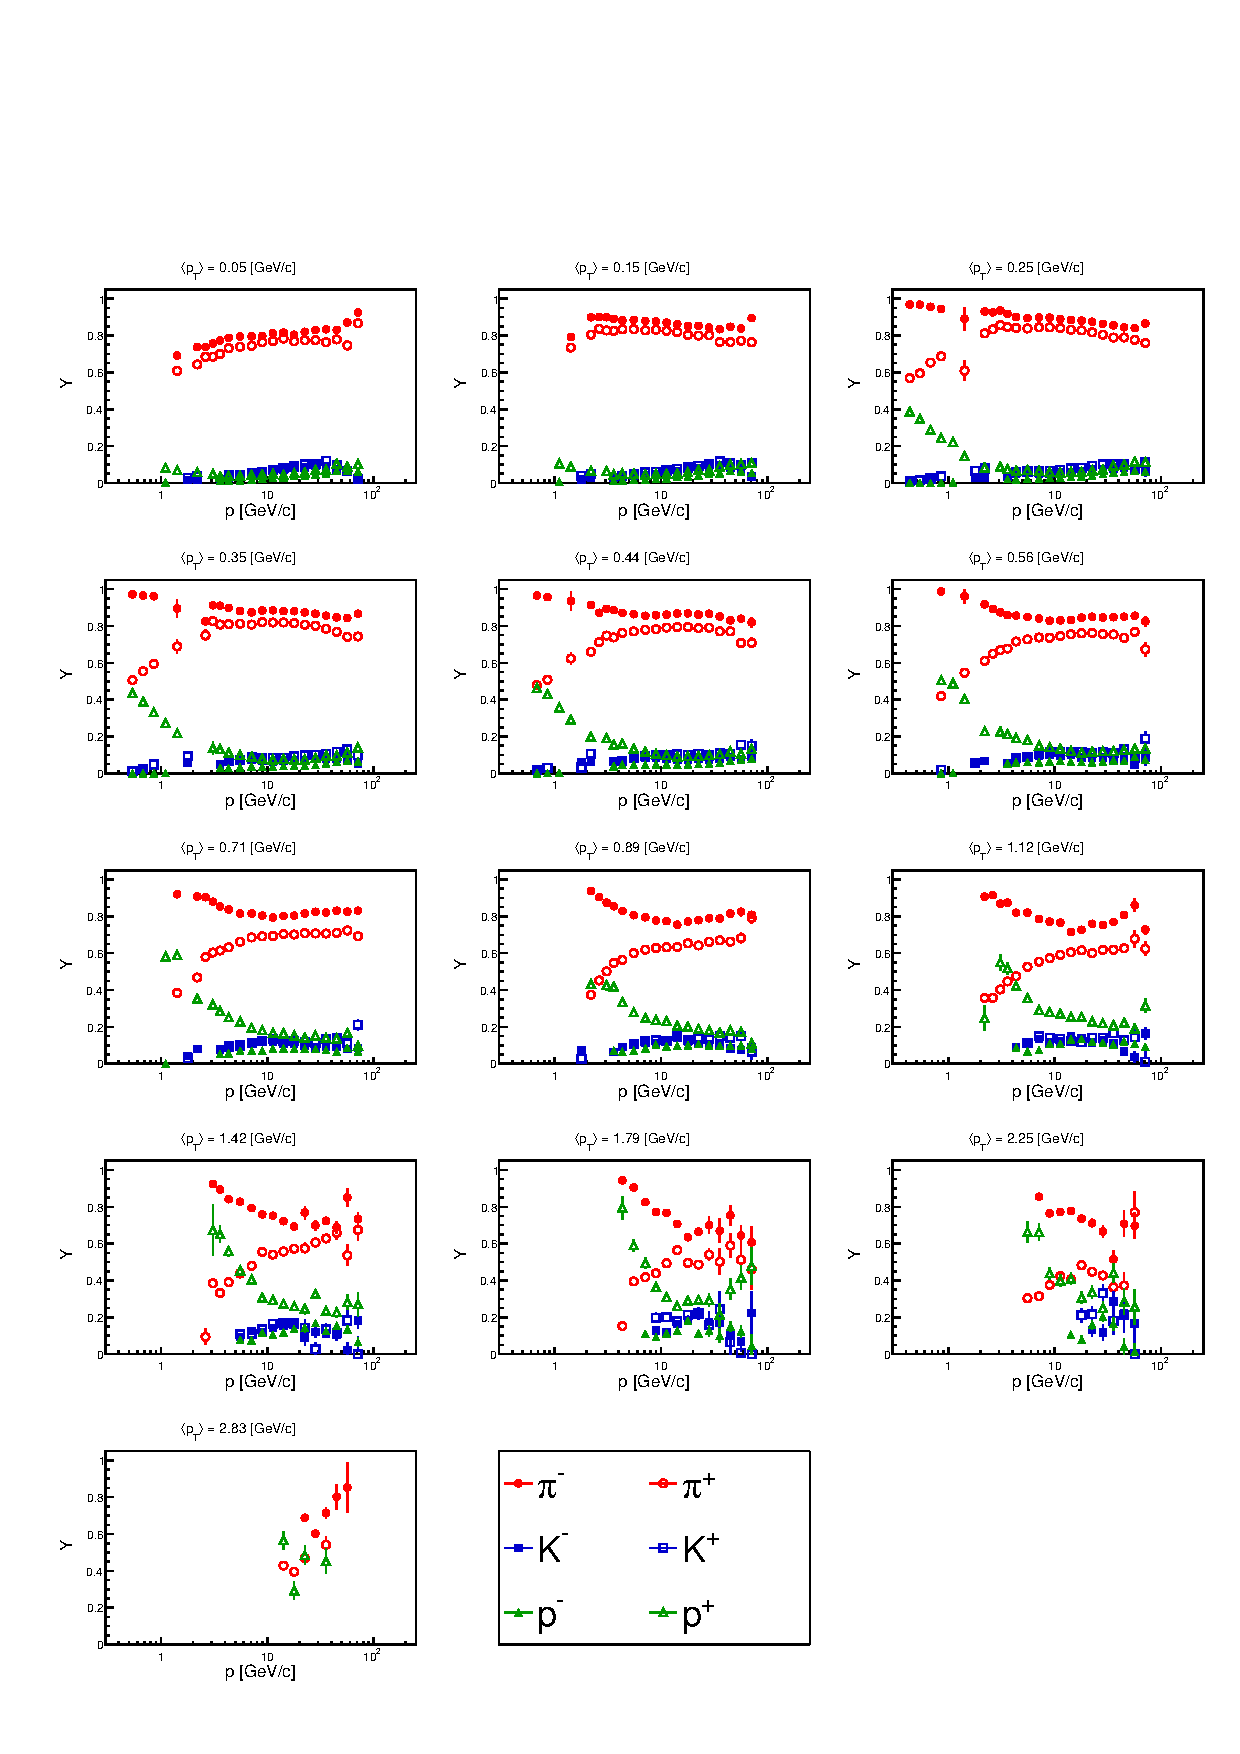
\includegraphics[clip, rviewport=0 0 1 1,width=1.00\textwidth]{dedx/fraction_pt_158_fl2_v1}
  \caption{Particle fractions obtained from the \dedx fit,
    after applying the cuts and corrections (see~\cref{sec:hadron:dedx:sde}),
    of the WST and 158 \GeVc data set, with target inserted. Markers with different
    colors show particle types and negatively (positively) charged particles are shown
    in full (open) symbols. The $\langle\pT\rangle$ is indicated on the top of each plot.}
  \label{fig:hadron:dedx:fit:final158w}
\end{figure}

\begin{figure}
  \centering
  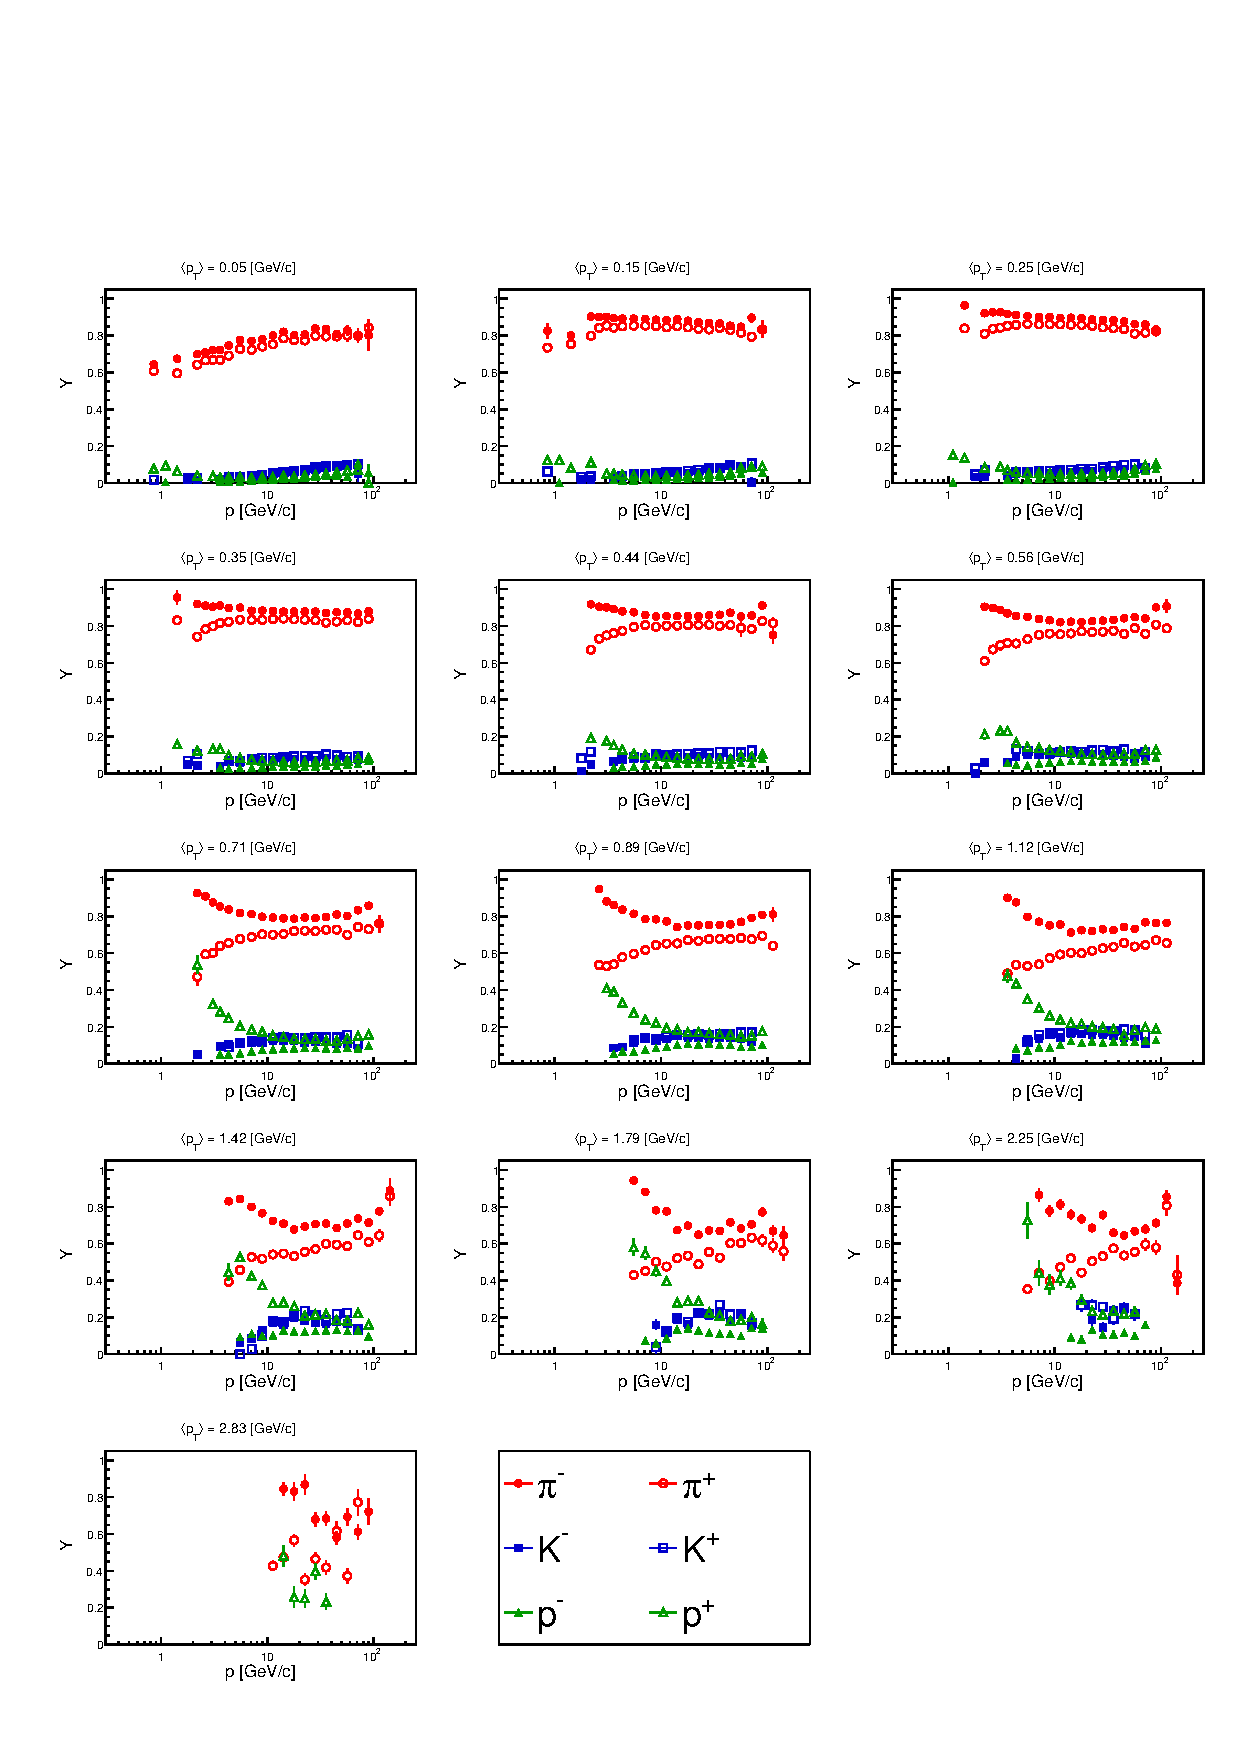
\includegraphics[clip, rviewport=0 0 1 1,width=1.00\textwidth]{dedx/fraction_pt_350_fl2_v0}
  \caption{Particle fractions obtained from the \dedx fit,
    after applying the cuts and corrections (see~\cref{sec:hadron:dedx:sde}),
    of the RST and 350 \GeVc data set, with target inserted. Markers with different
    colors show particle types and negatively (positively) charged particles are shown
    in full (open) symbols. The $\langle\pT\rangle$ is indicated on the top of each plot.}
  \label{fig:hadron:dedx:fit:final350r}
\end{figure}

\begin{figure}
  \centering
  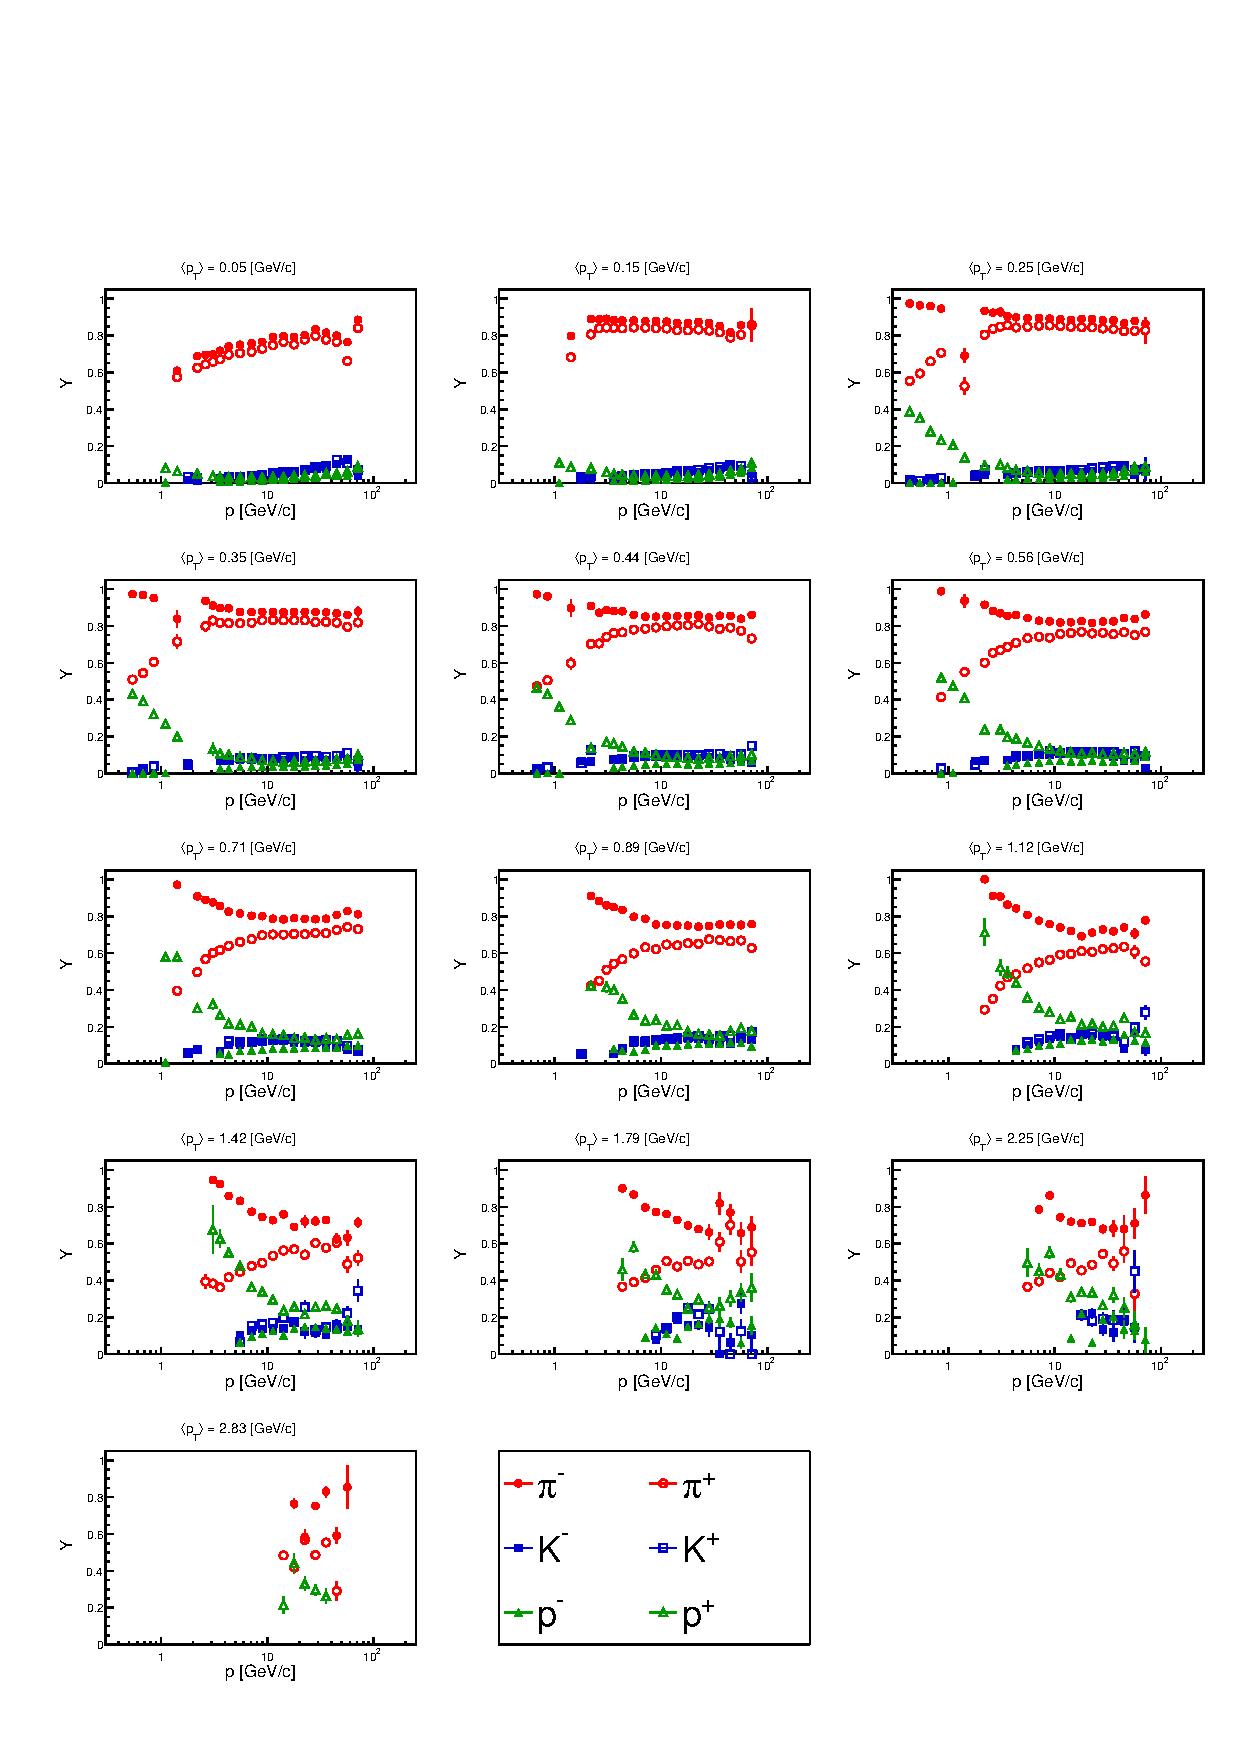
\includegraphics[clip, rviewport=0 0 1 1,width=1.00\textwidth]{dedx/fraction_pt_350_fl2_v1}
  \caption{Particle fractions obtained from the \dedx fit,
    after applying the cuts and corrections (see~\cref{sec:hadron:dedx:sde}),
    of the WST and 350 \GeVc data set, with target inserted. Markers with different
    colors show particle types and negatively (positively) charged particles are shown
    in full (open) symbols. The $\langle\pT\rangle$ is indicated on the top of each plot.}
  \label{fig:hadron:dedx:fit:final350w}
\end{figure}

%%%%%%%%%% FRACTION OUT%%%%%%%%%%%%%%
\begin{figure}
  \centering
  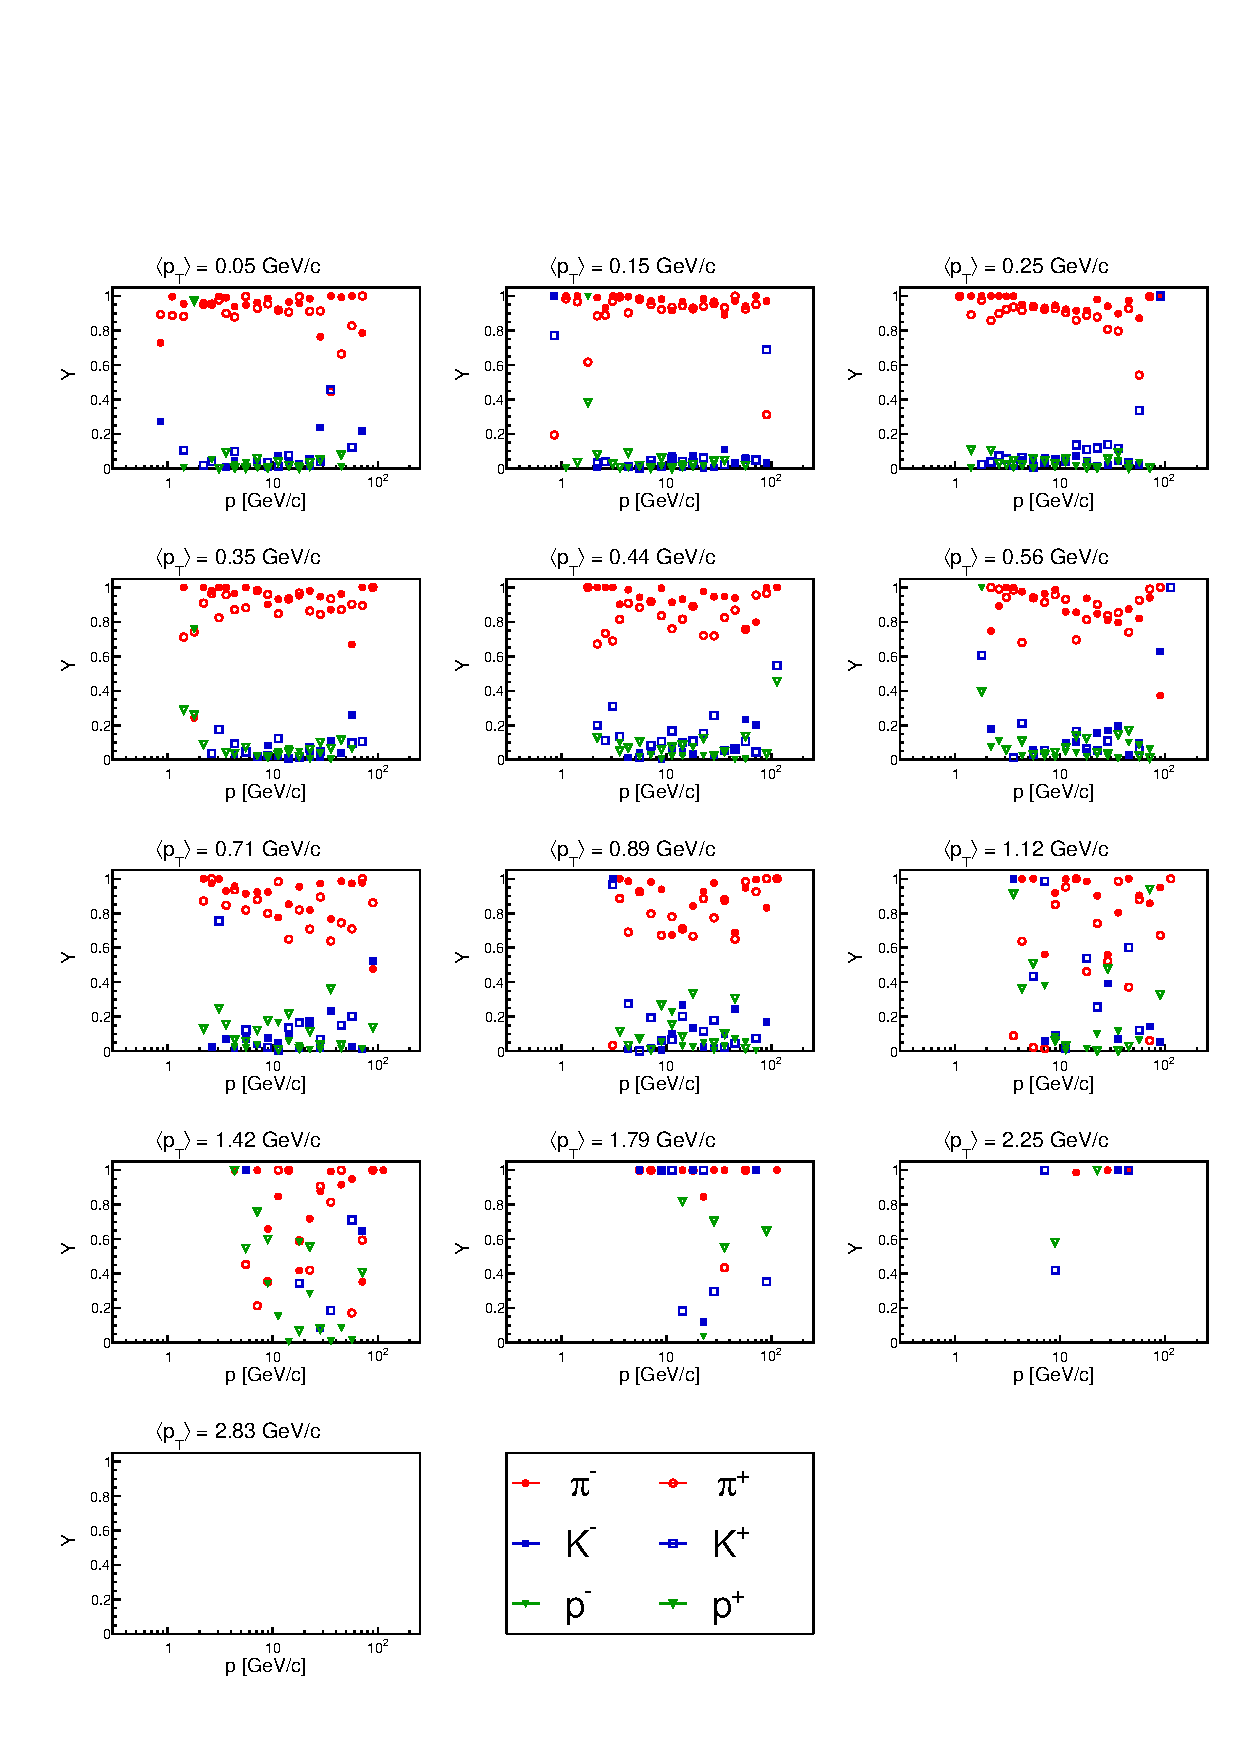
\includegraphics[clip, rviewport=0 0 1 1,width=1.00\textwidth]{dedx/fraction_out_pt_158_v0}
  \caption{Particle fractions obtained from the \dedx fit,
    after applying the cuts and corrections (see~\cref{sec:hadron:dedx:sde}),
    of the RST and 158 \GeVc data set, with target removed. Markers with different
    colors show particle types and negatively (positively) charged particles are shown
    in full (open) symbols. The $\langle\pT\rangle$ is indicated on the top of each plot.}
  \label{fig:hadron:dedx:fit:out158r}
\end{figure}

\begin{figure}
  \centering
  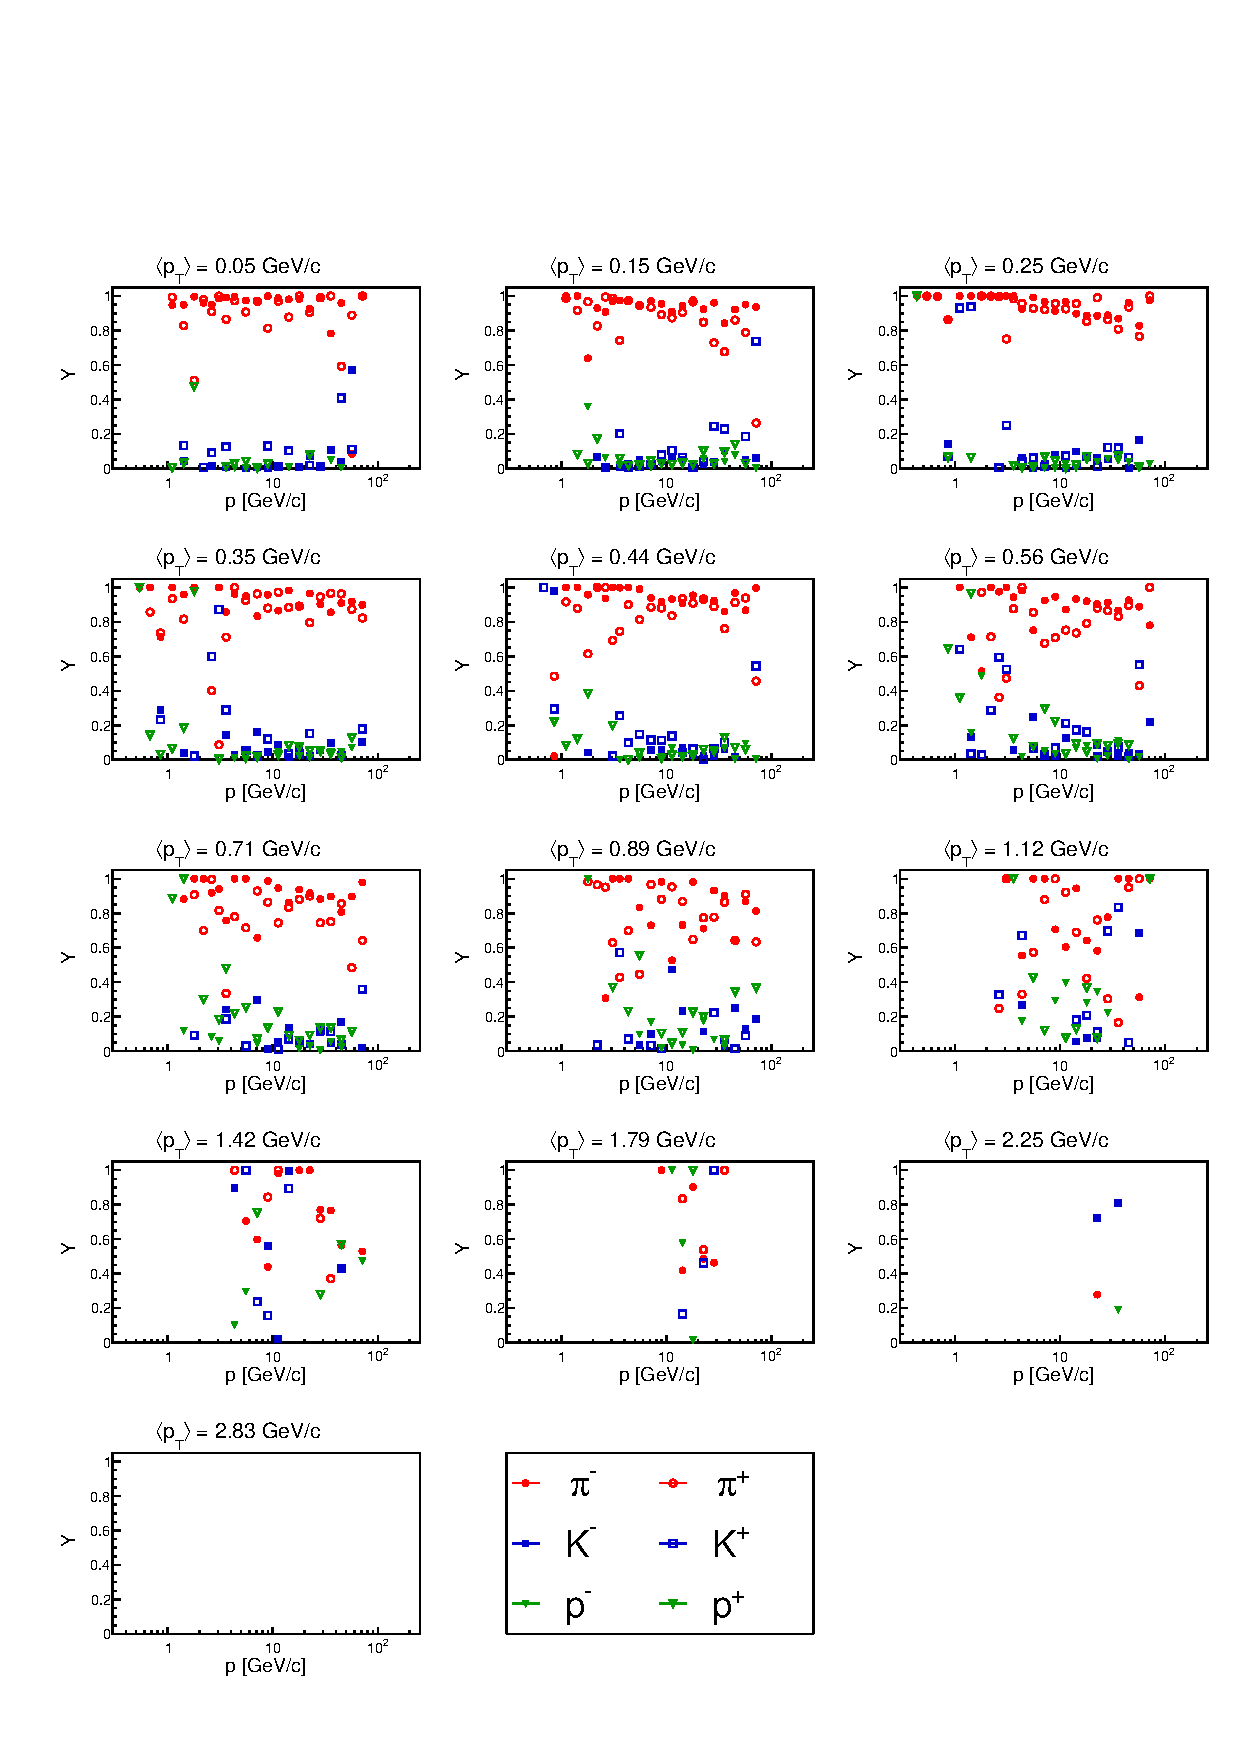
\includegraphics[clip, rviewport=0 0 1 1,width=1.00\textwidth]{dedx/fraction_out_pt_158_v1}
  \caption{Particle fractions obtained from the \dedx fit,
    after applying the cuts and corrections (see~\cref{sec:hadron:dedx:sde}),
    of the WST and 158 \GeVc data set, with target removed. Markers with different
    colors show particle types and negatively (positively) charged particles are shown
    in full (open) symbols. The $\langle\pT\rangle$ is indicated on the top of each plot.}
  \label{fig:hadron:dedx:fit:out158w}
\end{figure}

\begin{figure}
  \centering
  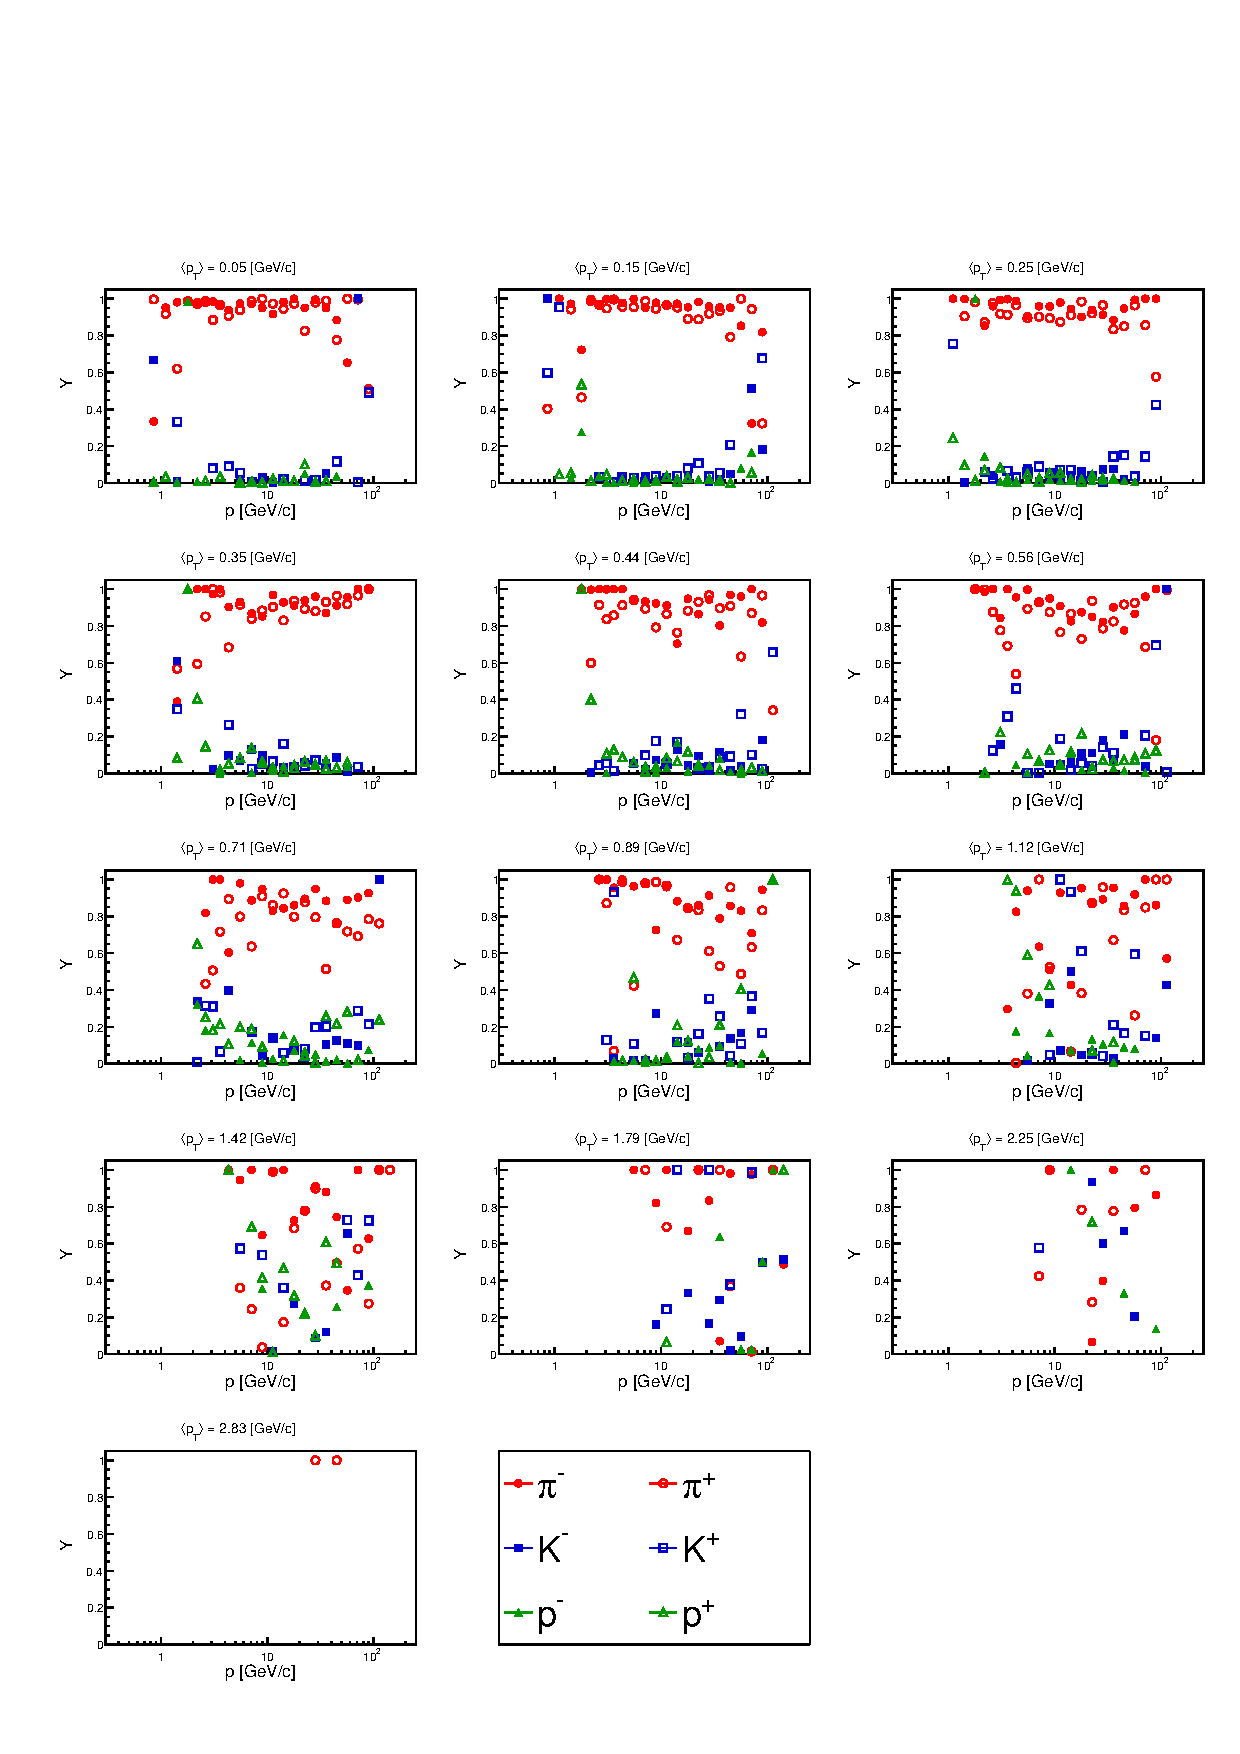
\includegraphics[clip, rviewport=0 0 1 1,width=1.00\textwidth]{dedx/fraction_out_pt_350_v0}
  \caption{Particle fractions obtained from the \dedx fit,
    after applying the cuts and corrections (see~\cref{sec:hadron:dedx:sde}),
    of the RST and 350 \GeVc data set, with target removed. Markers with different
    colors show particle types and negatively (positively) charged particles are shown
    in full (open) symbols. The $\langle\pT\rangle$ is indicated on the top of each plot.}
  \label{fig:hadron:dedx:fit:out350r}
\end{figure}

\begin{figure}
  \centering
  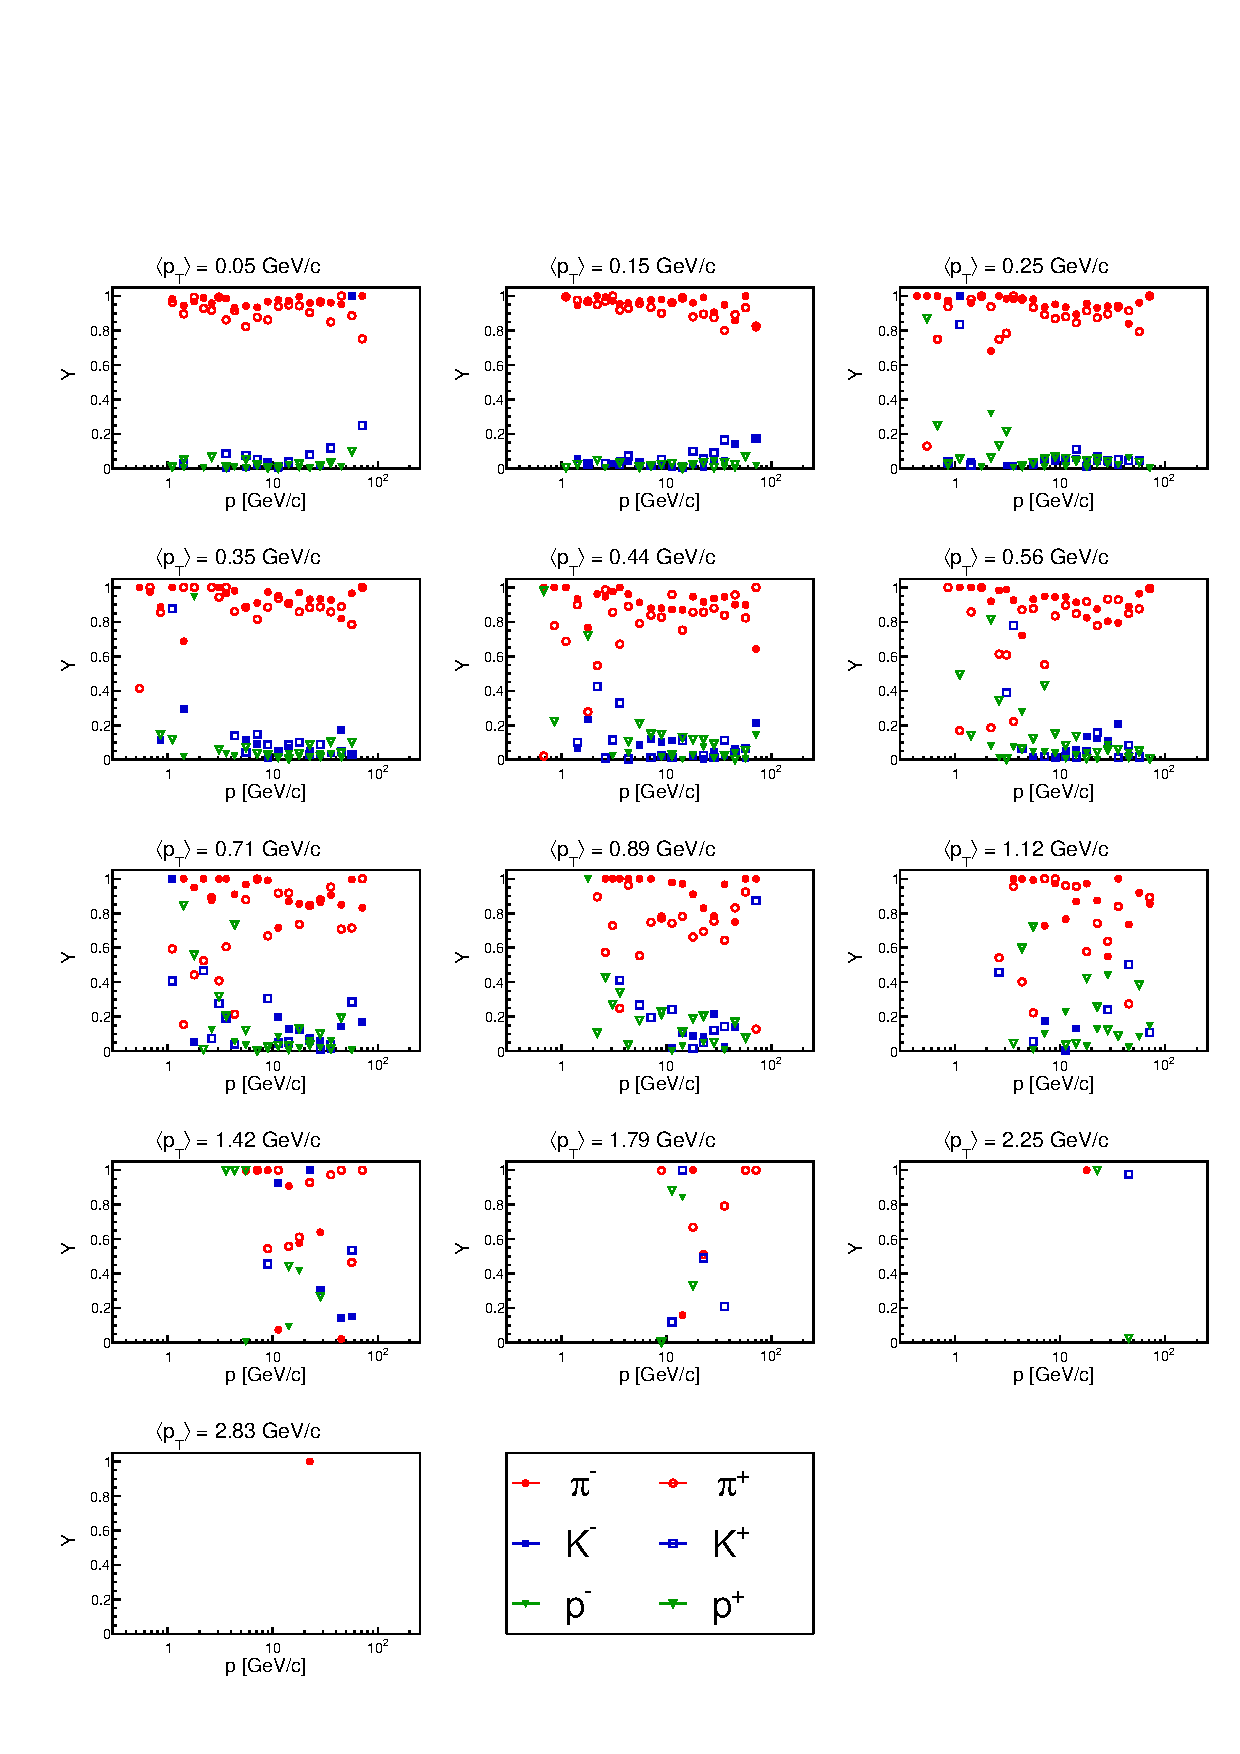
\includegraphics[clip, rviewport=0 0 1 1,width=1.00\textwidth]{dedx/fraction_out_pt_350_v1}
  \caption{Particle fractions obtained from the \dedx fit,
    after applying the cuts and corrections (see~\cref{sec:hadron:dedx:sde}),
    of the WST and 350 \GeVc data set, with target removed. Markers with different
    colors show particle types and negatively (positively) charged particles are shown
    in full (open) symbols. The $\langle\pT\rangle$ is indicated on the top of each plot.}
  \label{fig:hadron:dedx:fit:out350w}
\end{figure}

%%%%%%%%%%% DECAY DIST CUT %%%%%%%%%%%%%%%%%%
\begin{figure}
  \centering

  \begin{overpic}[clip, rviewport=0 0 1 1,width=0.99\textwidth]{vzero/cut_dist_Data350}
    \put(28,20){(a)}
    \put(61,20){(b)}
    \put(95,20){(c)}
  \end{overpic}

  \caption{Optimization of the \decaydistmin for the 350 \GeVc data set.
    The \lamb case is shown in (a), \antilamb in (b) and \kzeros in (c).
    Individual phase space bins are shown as black markers, the average over
    \pT bins is shown as red markers.}
  \label{fig:hadron:vzero:cuts:decaydist:350}
\end{figure}


\clearpage

%%%%%%%%%%% DIST IN %%%%%%%%%%%%%%%%%%
\begin{figure}[!ht]
  \centering
  \begin{overpic}[clip, rviewport=0 0 1 1,width=0.32\textwidth]{vzero/mass_Data350_t0_ph1_h0_x1_y3}
    \put(14,86){(a) \lamb}
  \end{overpic}
  \begin{overpic}[clip, rviewport=0 0 1 1,width=0.32\textwidth]{vzero/mass_Data350_t0_ph1_h1_x1_y3}
    \put(14,86){(b) \antilamb}
  \end{overpic}
  \begin{overpic}[clip, rviewport=0 0 1 1,width=0.32\textwidth]{vzero/mass_Data350_t0_ph1_h2_x2_y4}
    \put(14,86){(c) \kzeros}
  \end{overpic}

  \vspace{0.5cm}
  
  \begin{overpic}[clip, rviewport=0 0 1 1,width=0.32\textwidth]{vzero/mass_Data350_t0_ph1_h0_x5_y0}
    \put(14,86){(d) \lamb}
  \end{overpic}
  \begin{overpic}[clip, rviewport=0 0 1 1,width=0.32\textwidth]{vzero/mass_Data350_t0_ph1_h1_x5_y0}
    \put(14,86){(e) \antilamb}
  \end{overpic}
  \begin{overpic}[clip, rviewport=0 0 1 1,width=0.32\textwidth]{vzero/mass_Data350_t0_ph1_h2_x5_y1}
    \put(14,86){(f) \kzeros}
  \end{overpic}

  \caption{Examples of the fitted \minv distributions for the 350 \GeVc data set with target inserted.
    Two phase space bins are shown for \lamb in (a) and (d),
    for \antilamb in (b) and (e) and for \kzeros in (c) and (f).
    The black markers show the measured \minv distributions. The colored curves show
    the results of the fit, being the signal in blue, the background in red and the total in gray.
    Additionally, in green and purple we show the contributions of the two separated templates.
    On the bottom of each plot we show the residual distributions, being $\Delta$ the difference
    between observed and fitted number of entries and $\sigma$ the uncertainties of the observed number.
    The $\langle\pp\rangle$ and $\langle\pT\rangle$ of the phase space bin are
    indicated on the top of each plot.}
  \label{fig:hadron:vzero:signal:dist:350:in}
\end{figure}

%%%%%%%%%%% DIST OUT %%%%%%%%%%%%%%%%%%
\begin{figure}[!ht]
  \centering
  \begin{overpic}[clip, rviewport=0 0 1 1,width=0.32\textwidth]{vzero/mass_Data350_t1_ph0_h0_x3_y0}
    \put(14,86){(a) \lamb}
  \end{overpic}
  \begin{overpic}[clip, rviewport=0 0 1 1,width=0.32\textwidth]{vzero/mass_Data350_t1_ph0_h1_x3_y0}
    \put(14,86){(b) \antilamb}
  \end{overpic}
  \begin{overpic}[clip, rviewport=0 0 1 1,width=0.32\textwidth]{vzero/mass_Data350_t1_ph0_h2_x3_y0}
    \put(14,86){(c) \kzeros}
  \end{overpic}

  \caption{Examples of the fitted \minv distributions for the 350 \GeVc data set with target removed.
    One \pp bin is shown for \lamb in (a), for \antilamb in (b) and for \kzeros in (c).
    The black markers show the measured \minv distributions. The colored curves show
    the results of the fit, being the signal in blue, the background in red and the total in gray.
    On the bottom of each plot we show the residual distributions, being $\Delta$ the difference
    between observed and fitted number of entries and $\sigma$ the uncertainties of the observed number.
    The $\langle\pp\rangle$ of the phase space bin is indicated on the top of each plot.}
  \label{fig:hadron:vzero:signal:dist:350:out}
\end{figure}

\clearpage

%%%%%%%%%%% CHI SQ IN %%%%%%%%%%%%%%%%%%
\begin{figure}[!ht]
  \centering

  \begin{overpic}[clip, rviewport=0 0 1 1,width=0.99\textwidth]{vzero/chisq_Data350_t0_ph1}
    \put(6,20){(a)\lamb}
    \put(39.5,20){(b)\antilamb}
    \put(72.5,20){(c)\kzeros}
  \end{overpic}

  \vspace{0.5cm}

\begin{overpic}[clip, rviewport=0 0 1 1,width=0.99\textwidth]{vzero/chisq_Data350_t1_ph0}
    \put(6,20){(d)\lamb}
    \put(39.5,20){(e)\antilamb}
    \put(72.5,20){(f)\kzeros}
  \end{overpic}

  \caption{\redchisq of the \minv fit of the 350 \GeVc data set
    for the target inserted (upper plots) and removed (lower plots).
    The \lamb cases are shown in (a) and (d),
    the \antilamb in (b) and (e) and the \kzeros in (c) and (f).}
  \label{fig:hadron:vzero:signal:chi:350}
\end{figure}



%%%%%%%%%%% EXTRACTED SIGNAL %%%%%%%%%%%%%%%%%%
\begin{figure}[!ht]
  \centering
  \begin{overpic}[clip, rviewport=0 0 1 1,width=0.99\textwidth]{vzero/signal_Data350_t0}
    \put(6,20){(a)\lamb}
    \put(39.5,20){(b)\antilamb}
    \put(72.5,20){(c)\kzeros}
  \end{overpic}

  \vspace{0.5cm}
  
  \begin{overpic}[clip, rviewport=0 0 1 1,width=0.99\textwidth]{vzero/signal_Data350_t1}
    \put(6,20){(d)\lamb}
    \put(39.5,20){(e)\antilamb}
    \put(72.5,20){(f)\kzeros}
  \end{overpic}

  \caption{Extracted signal $S$ for the 350 \GeVc data set
    with target inserted (upper plots) and removed (lower plots).
    The \lamb cases are shown in (a) and (d),
    the \antilamb in (b) and (e) and the \kzeros in (c) and (f).}
  \label{fig:hadron:vzero:signal:extracted:350}
\end{figure}

\clearpage


%%%%%%%%%% BETA %%%%%%%%%%%%%%%%
\begin{figure}[!ht]
  \centering

  \begin{overpic}[clip, rviewport=0 0.143 1 1,width=0.45\textwidth]{dedx/fac_350_All_beta_c0_p1}
    \put(20,53){(a) $\pi^+$}
  \end{overpic}
  \begin{overpic}[clip, rviewport=0 0.143 1 1,width=0.45\textwidth]{dedx/fac_350_All_beta_c1_p1}
    \put(20,53){(b) $\pi^-$}
  \end{overpic}

  \begin{overpic}[clip, rviewport=0 0.143 1 1,width=0.45\textwidth]{dedx/fac_350_All_beta_c0_p2}
    \put(20,53){(c) K$^+$}
  \end{overpic}
  \begin{overpic}[clip, rviewport=0 0.143 1 1,width=0.45\textwidth]{dedx/fac_350_All_beta_c1_p2}
    \put(20,53){(d) K$^-$}
  \end{overpic}
  
  \begin{overpic}[clip, rviewport=0 0 1 1,width=0.45\textwidth]{dedx/fac_350_All_beta_c0_p3}
    \put(20,63){(e) p$^+$}
  \end{overpic}
  \begin{overpic}[clip, rviewport=0 0 1 1,width=0.45\textwidth]{dedx/fac_350_All_beta_c1_p3}
    \put(20,63){(f) p$^-$}
  \end{overpic}
    
  \caption{$\beta$ correction factor for the charged hadron analysis
    and for the 350 \GeVc data set. The $\pi^+$ case is shown in (a),
    $\pi^-$ in (b), K$^+$ in (c), K$^-$ in (d), p$^+$ in (e) and p$^-$ in (f).}
  \label{fig:hadron:correction:beta:dedx350}
\end{figure}


%%%%%%%%%%% BETA V0 %%%%%%%%%%%%%%%%%%
\begin{figure}[!ht]
  \centering

  \begin{overpic}[clip, rviewport=0 0 1 1,width=0.99\textwidth]{vzero/beta350}
    \put(0,22){(a)}
    \put(33,22){(b)}
    \put(67,22){(c)}
  \end{overpic}

  \caption{$\beta$ correction factor for the \vzero analysis
    and for the 350 \GeVc data set. The \lamb case is shown in (a),
    \antilamb in (b) and \kzeros in (c).}
  \label{fig:hadron:correction:beta:vzero350}
\end{figure}

\clearpage

%%%%%%%%%% SPEC PT ALL DEDX %%%%%%%%%%%%%%
\begin{figure}[!ht]
  \centering

  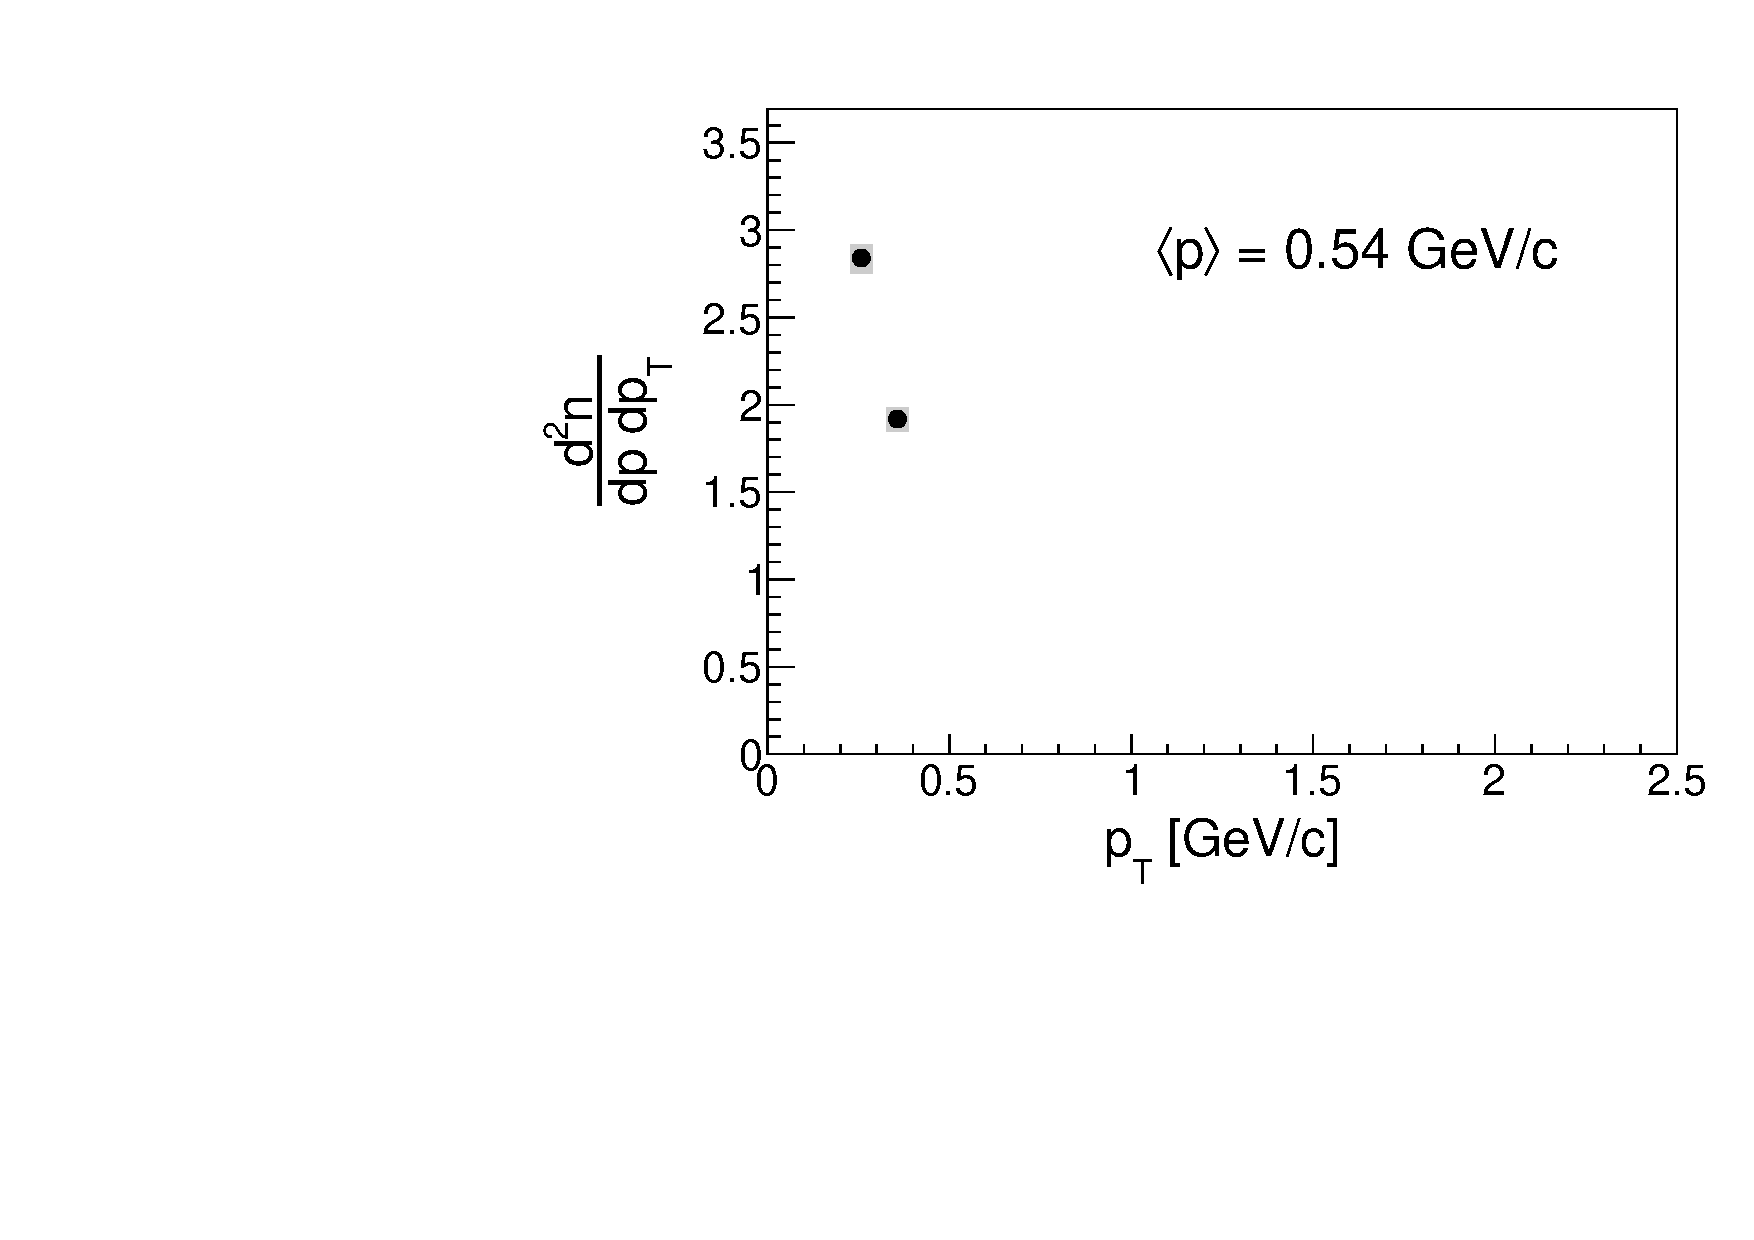
\includegraphics[clip, rviewport=0 0 1 1,width=0.24\textwidth]{spec/spec_pt_158_c0_p1_x7}
  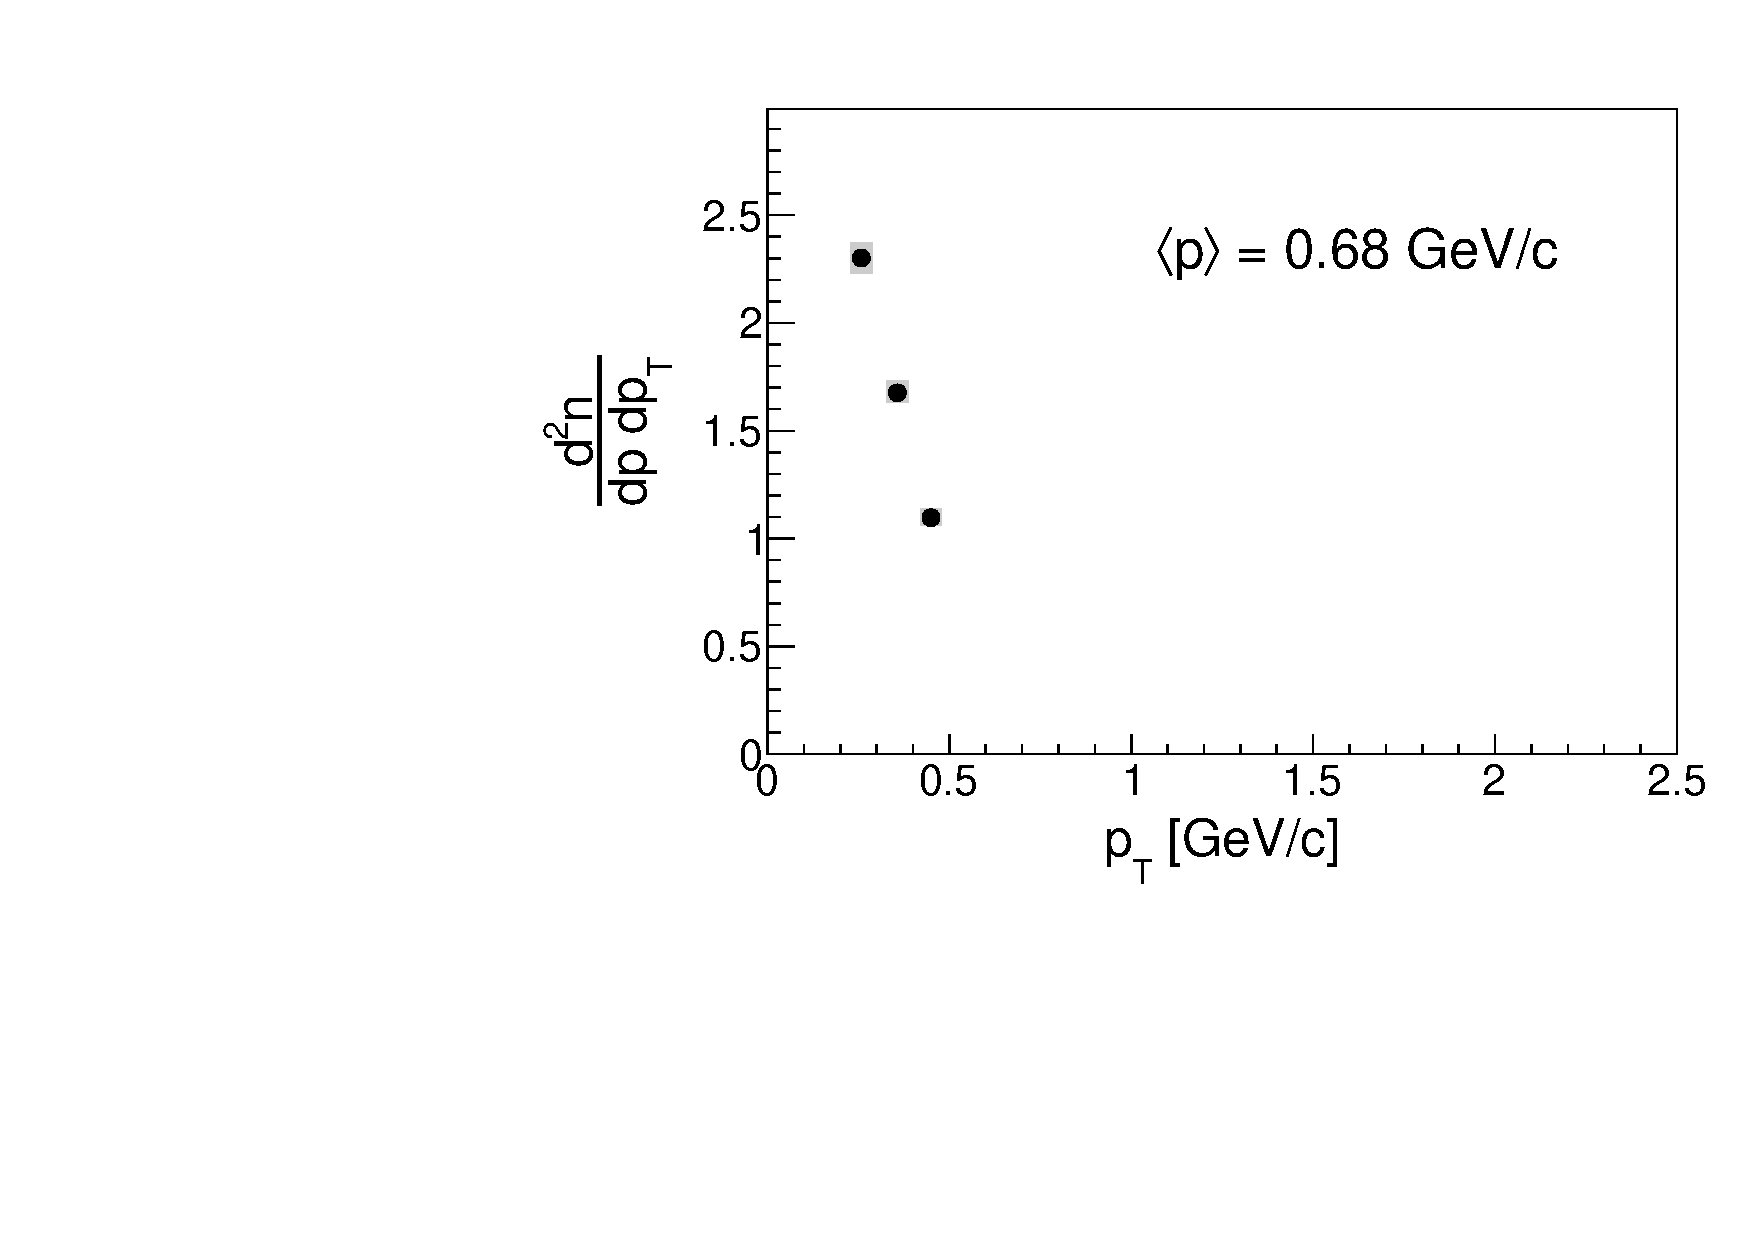
\includegraphics[clip, rviewport=0 0 1 1,width=0.24\textwidth]{spec/spec_pt_158_c0_p1_x8}
  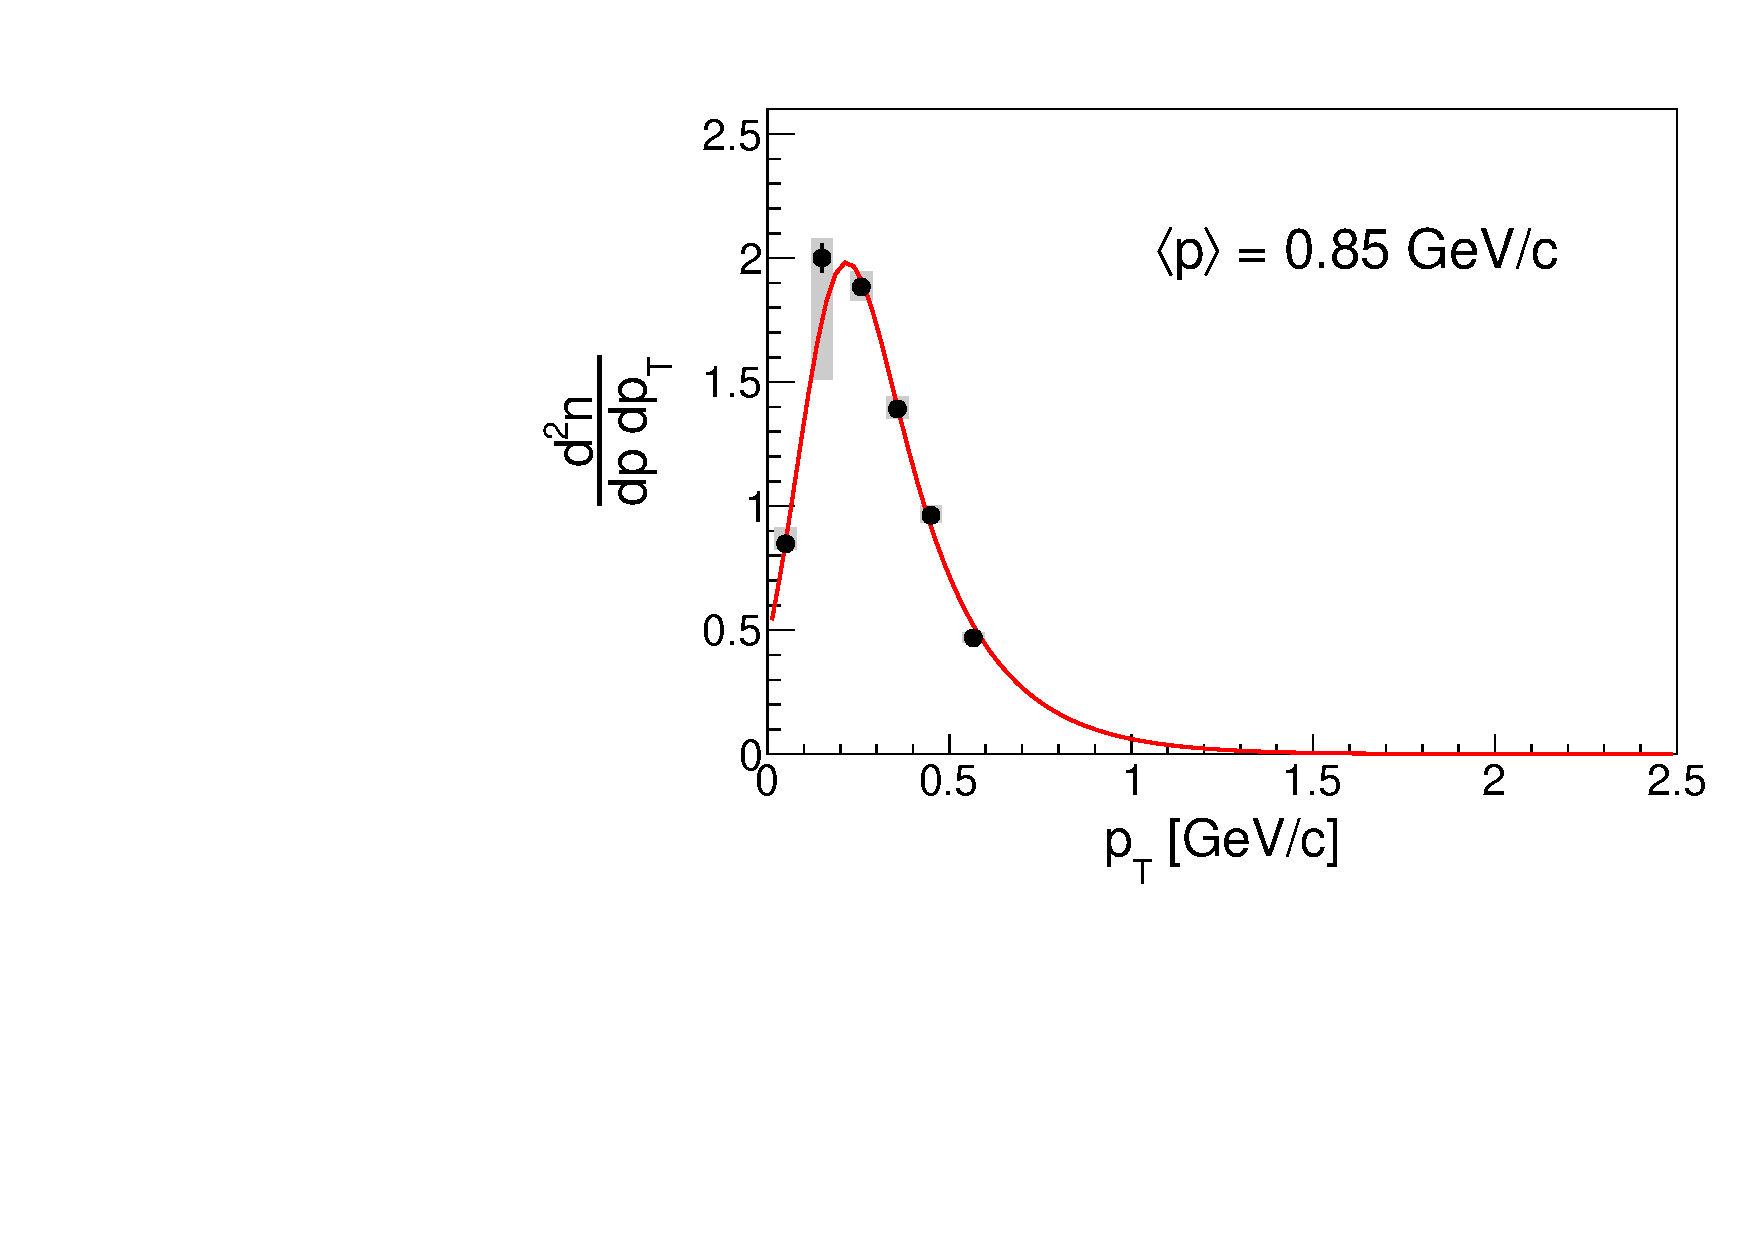
\includegraphics[clip, rviewport=0 0 1 1,width=0.24\textwidth]{spec/spec_pt_158_c0_p1_x9}
  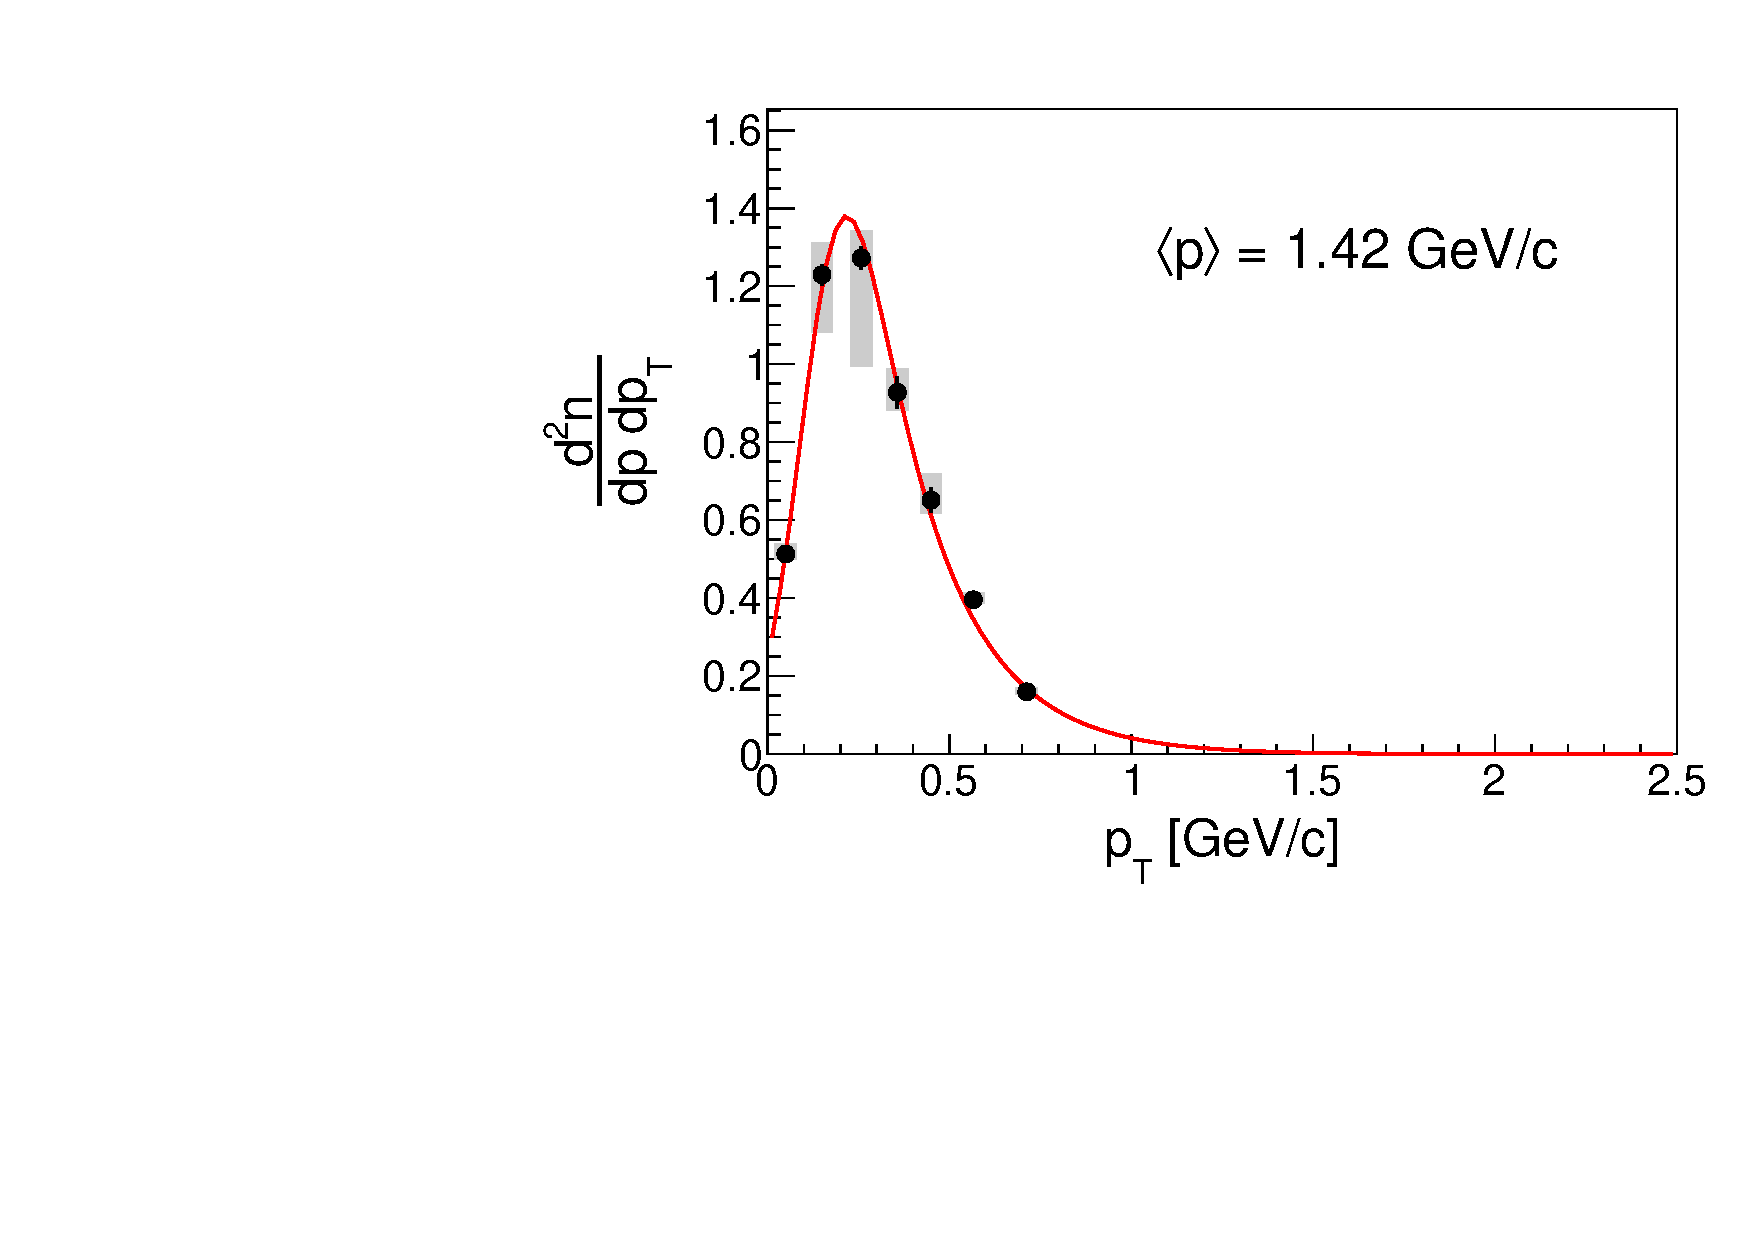
\includegraphics[clip, rviewport=0 0 1 1,width=0.24\textwidth]{spec/spec_pt_158_c0_p1_x11}

  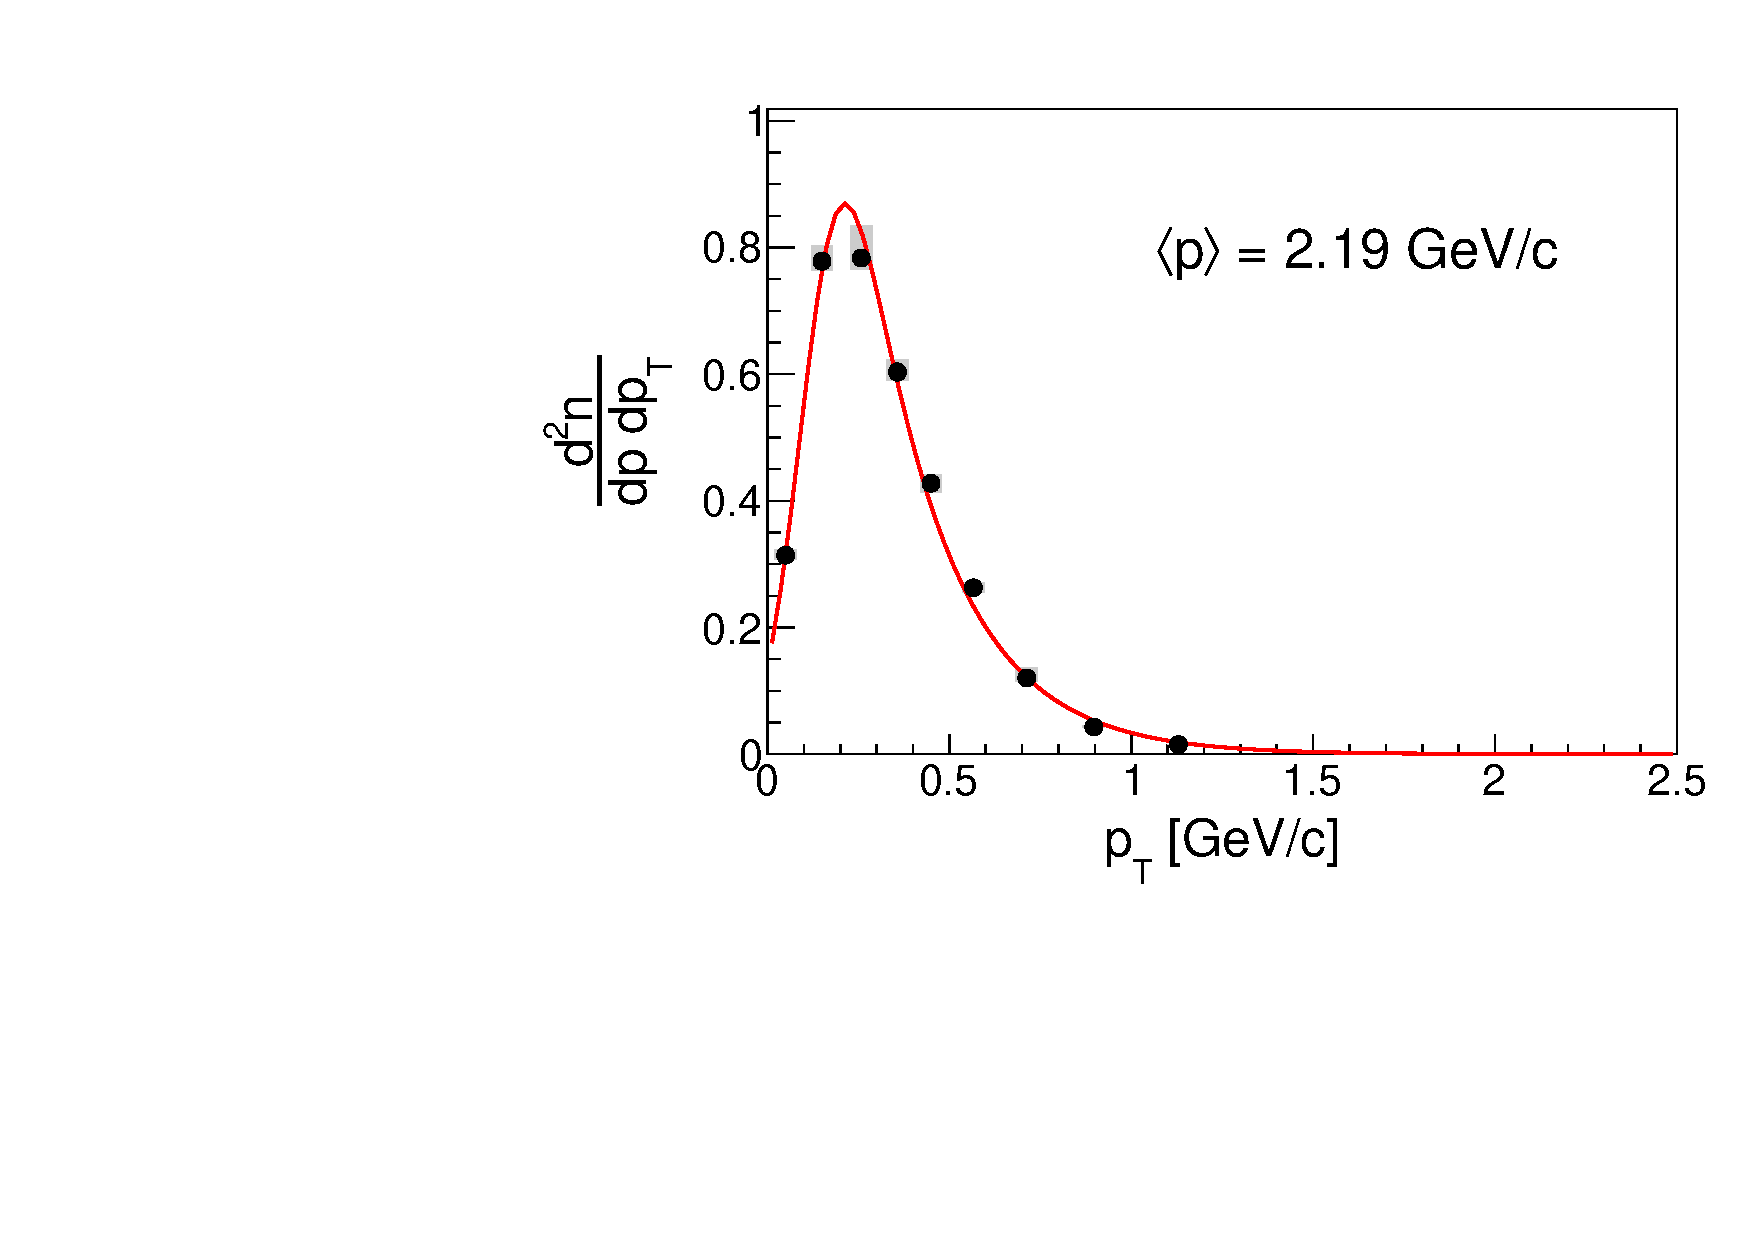
\includegraphics[clip, rviewport=0 0 1 1,width=0.24\textwidth]{spec/spec_pt_158_c0_p1_x13}
  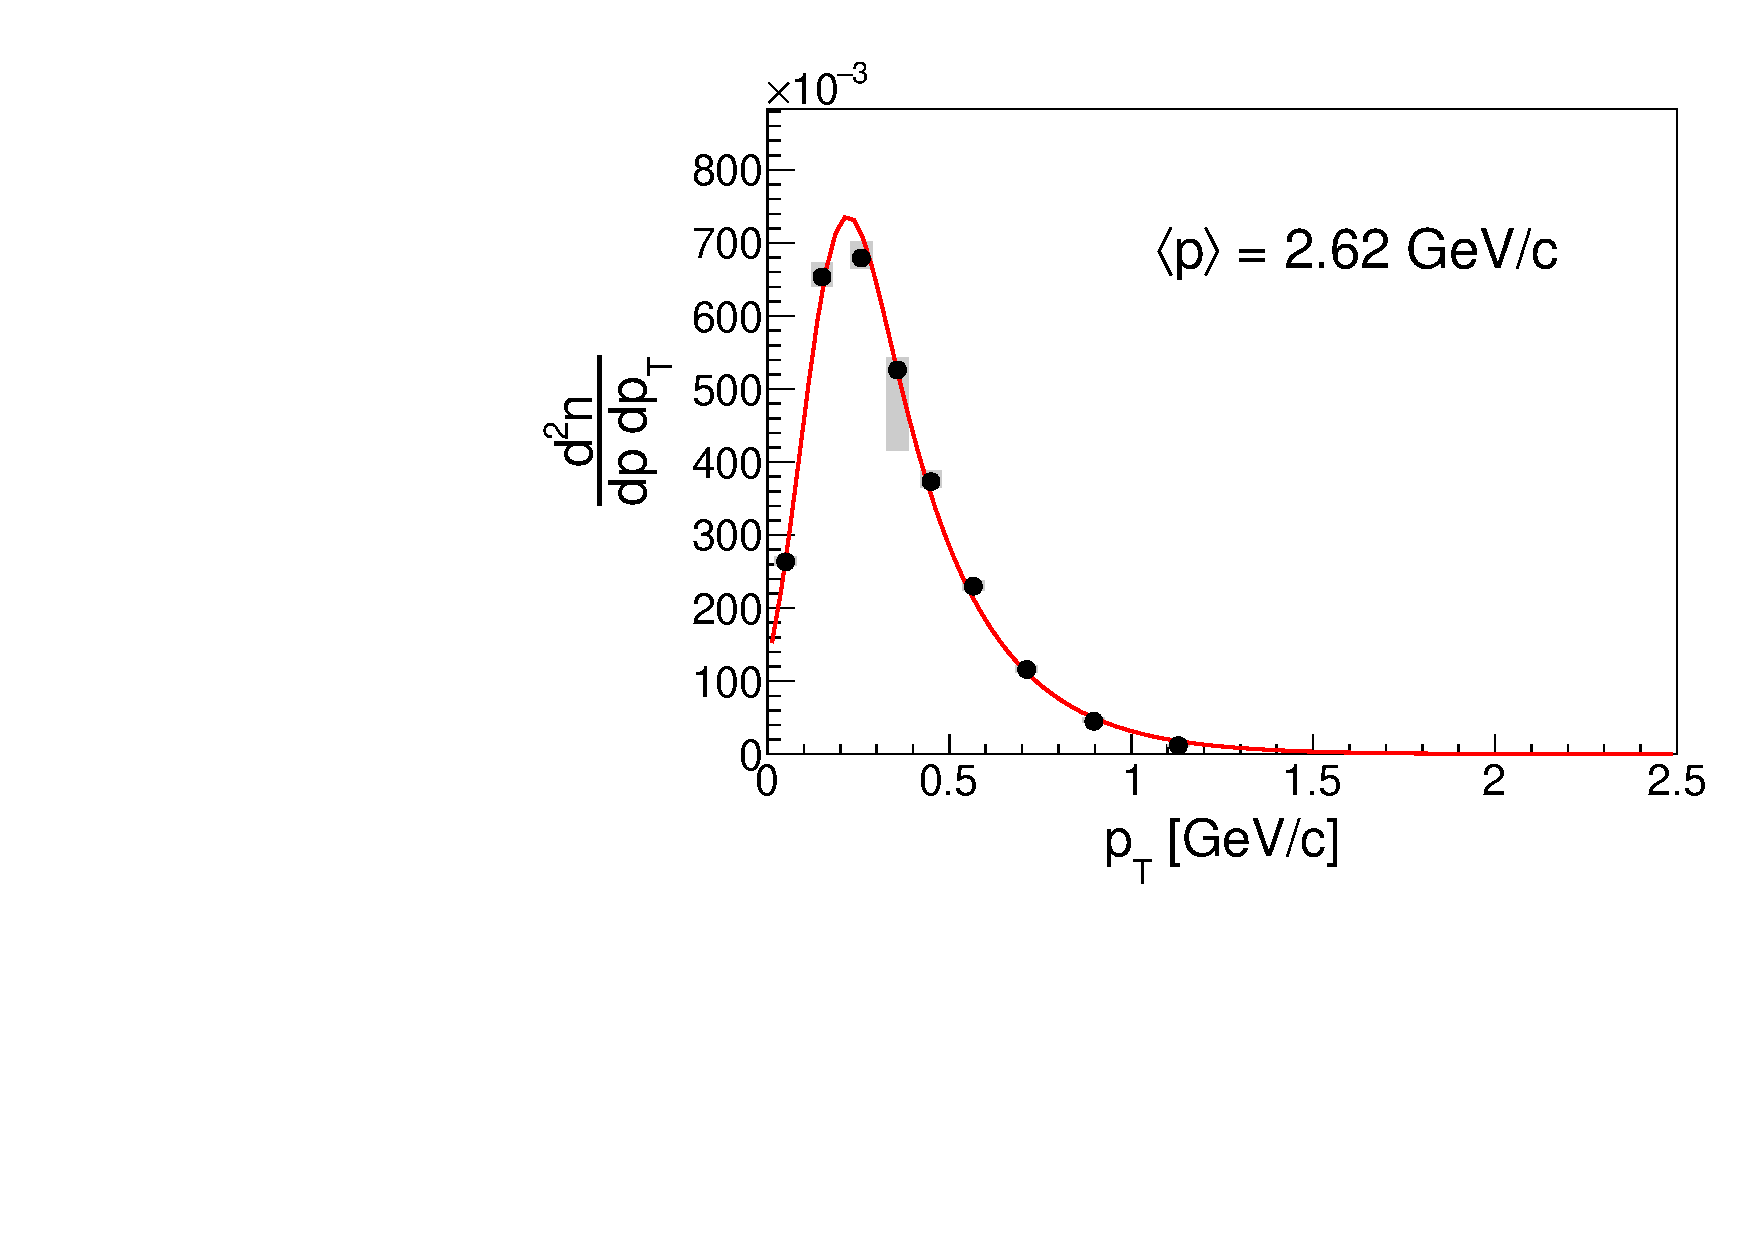
\includegraphics[clip, rviewport=0 0 1 1,width=0.24\textwidth]{spec/spec_pt_158_c0_p1_x14}
  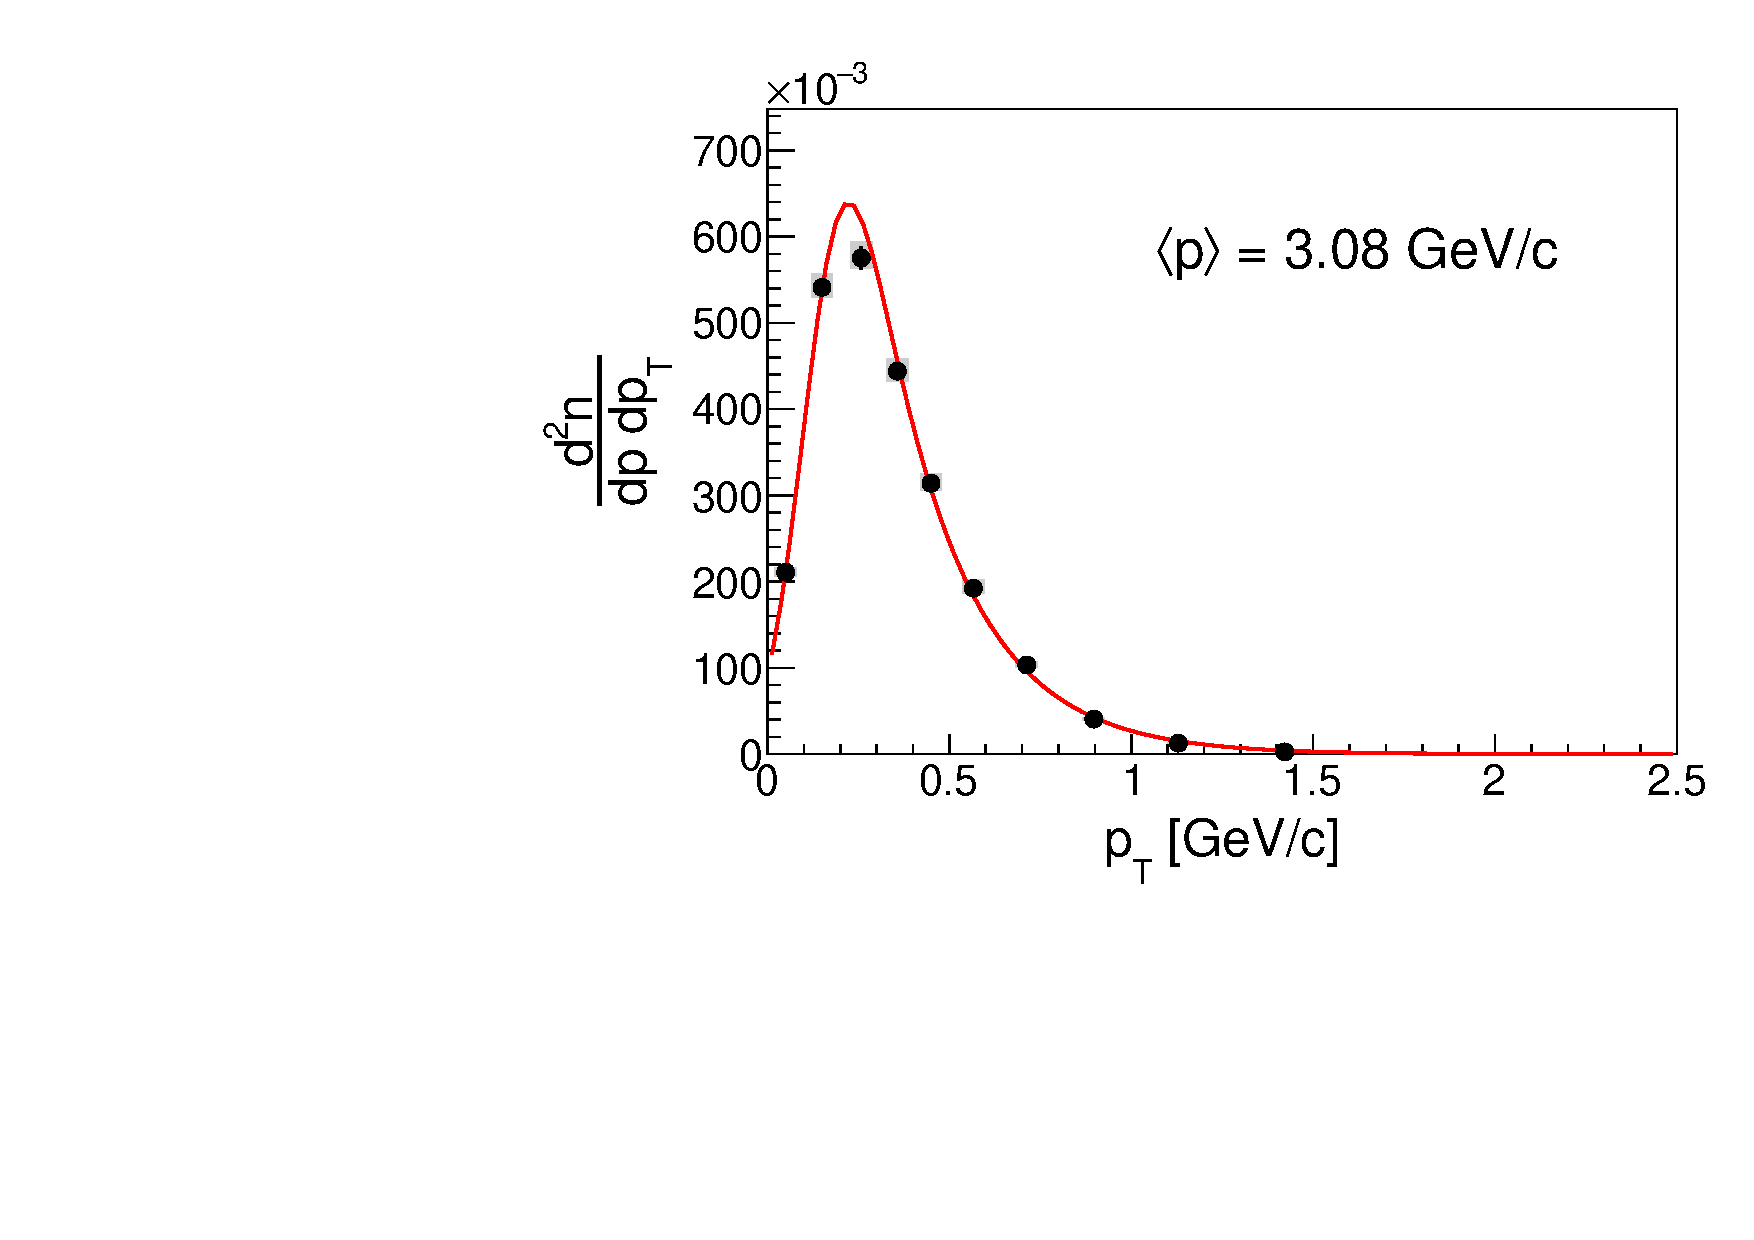
\includegraphics[clip, rviewport=0 0 1 1,width=0.24\textwidth]{spec/spec_pt_158_c0_p1_x15}
  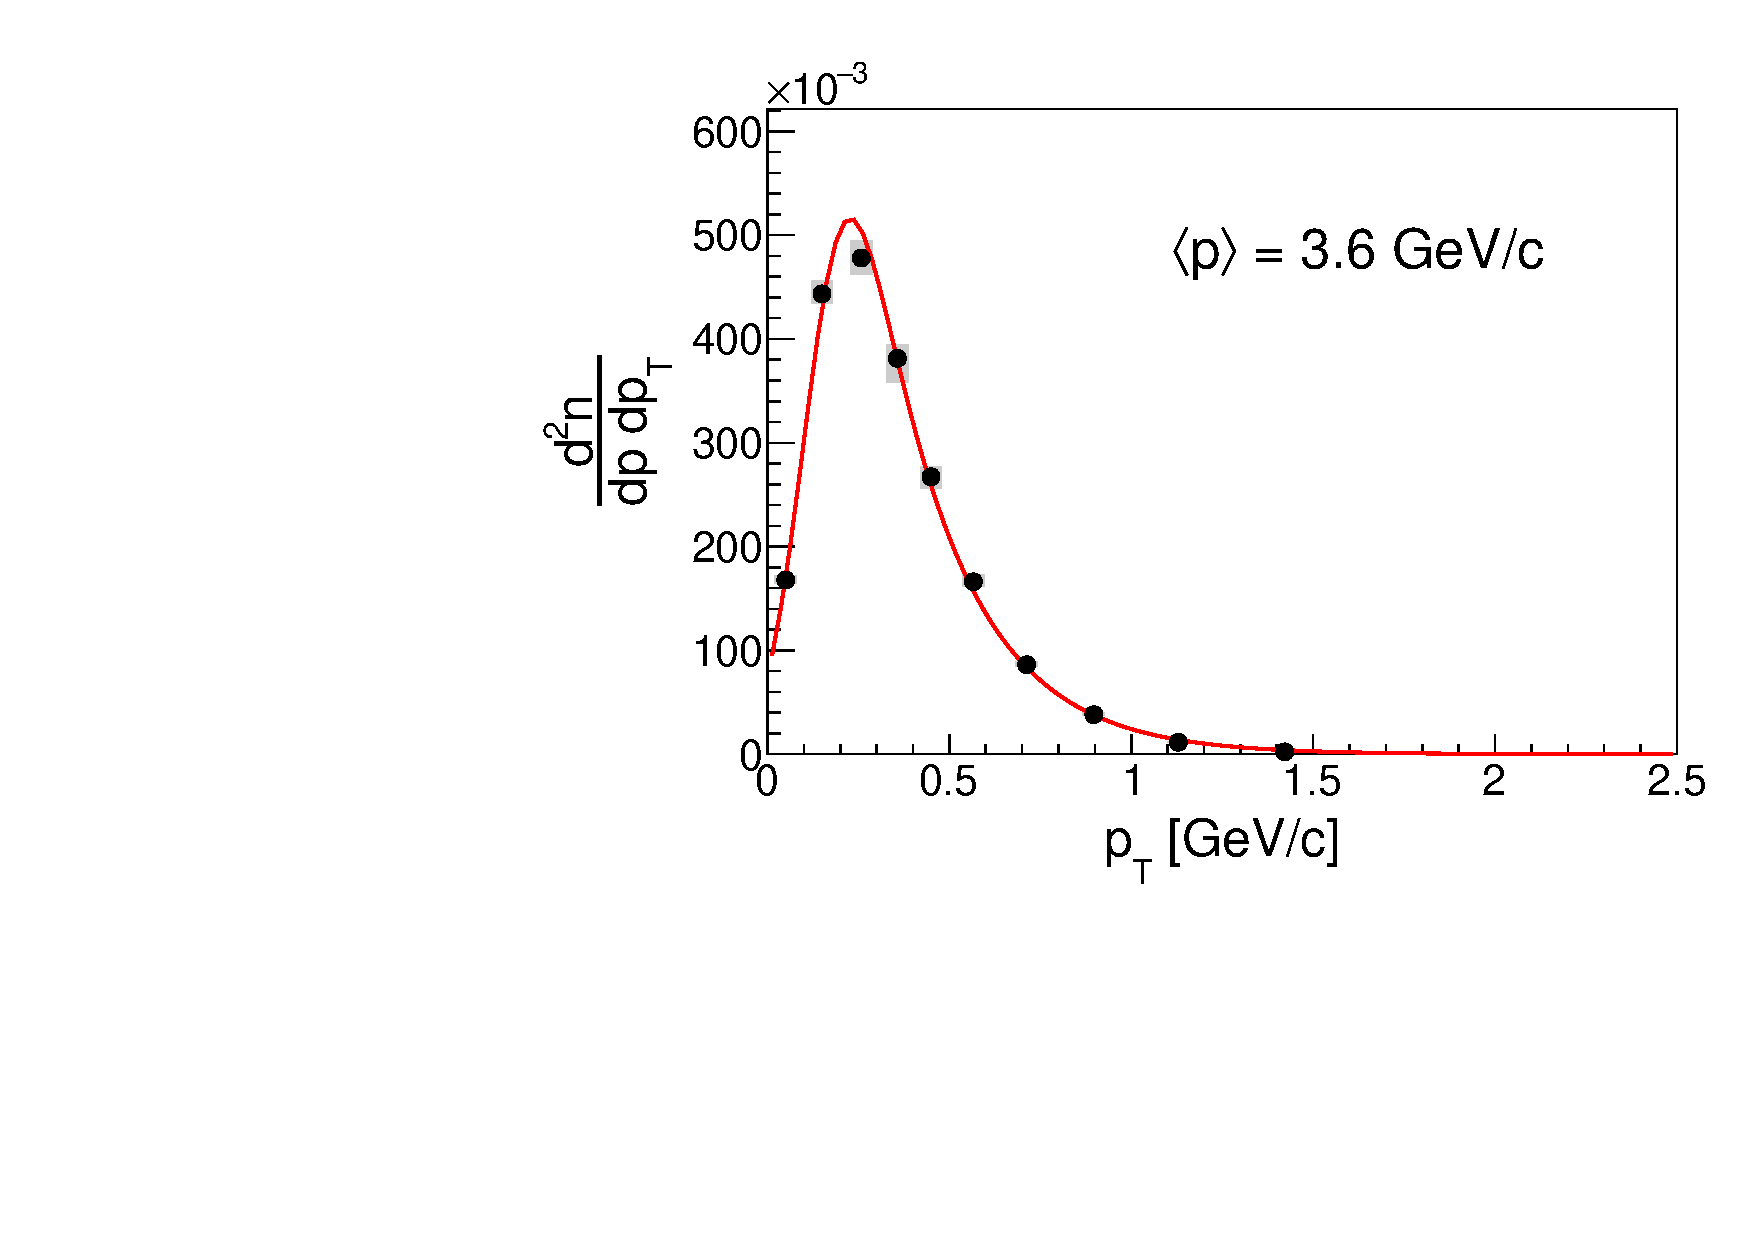
\includegraphics[clip, rviewport=0 0 1 1,width=0.24\textwidth]{spec/spec_pt_158_c0_p1_x16}

  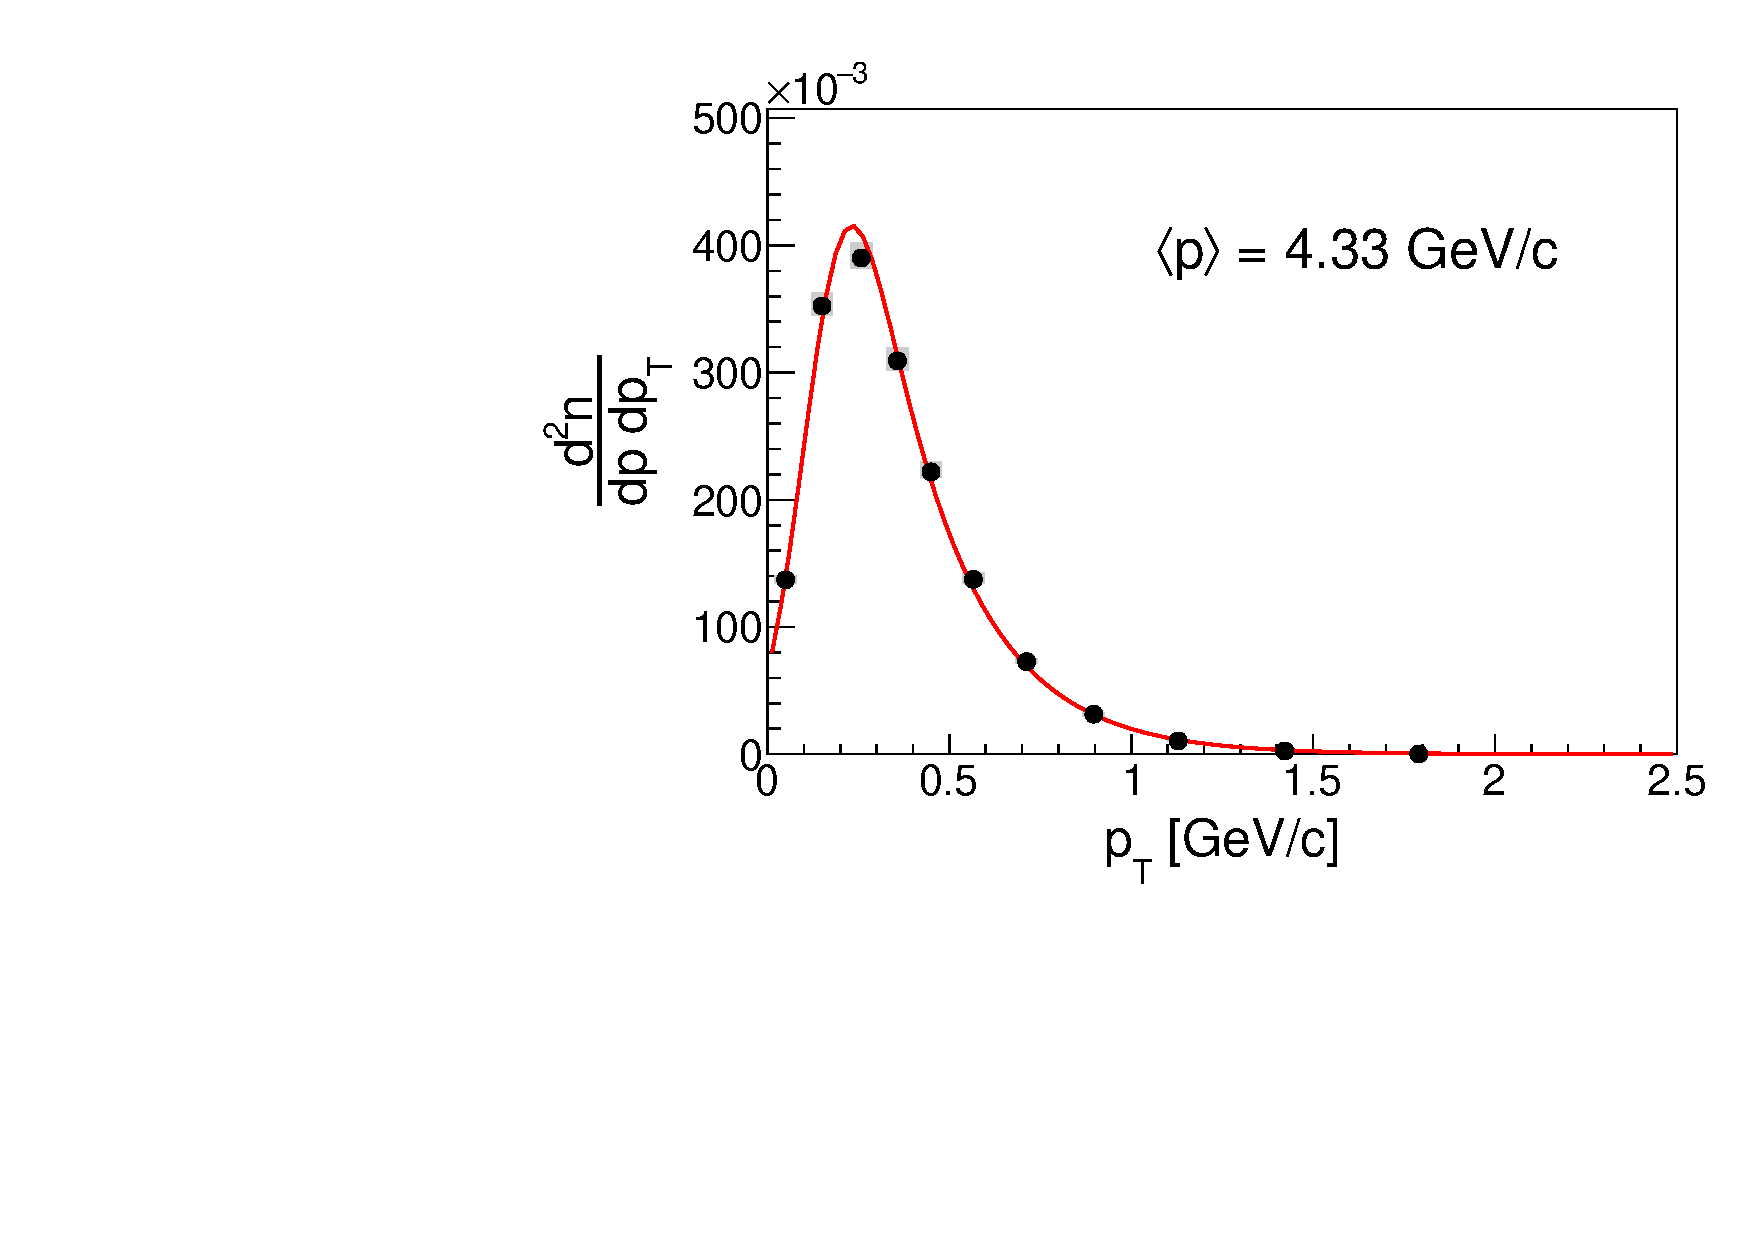
\includegraphics[clip, rviewport=0 0 1 1,width=0.24\textwidth]{spec/spec_pt_158_c0_p1_x17}
  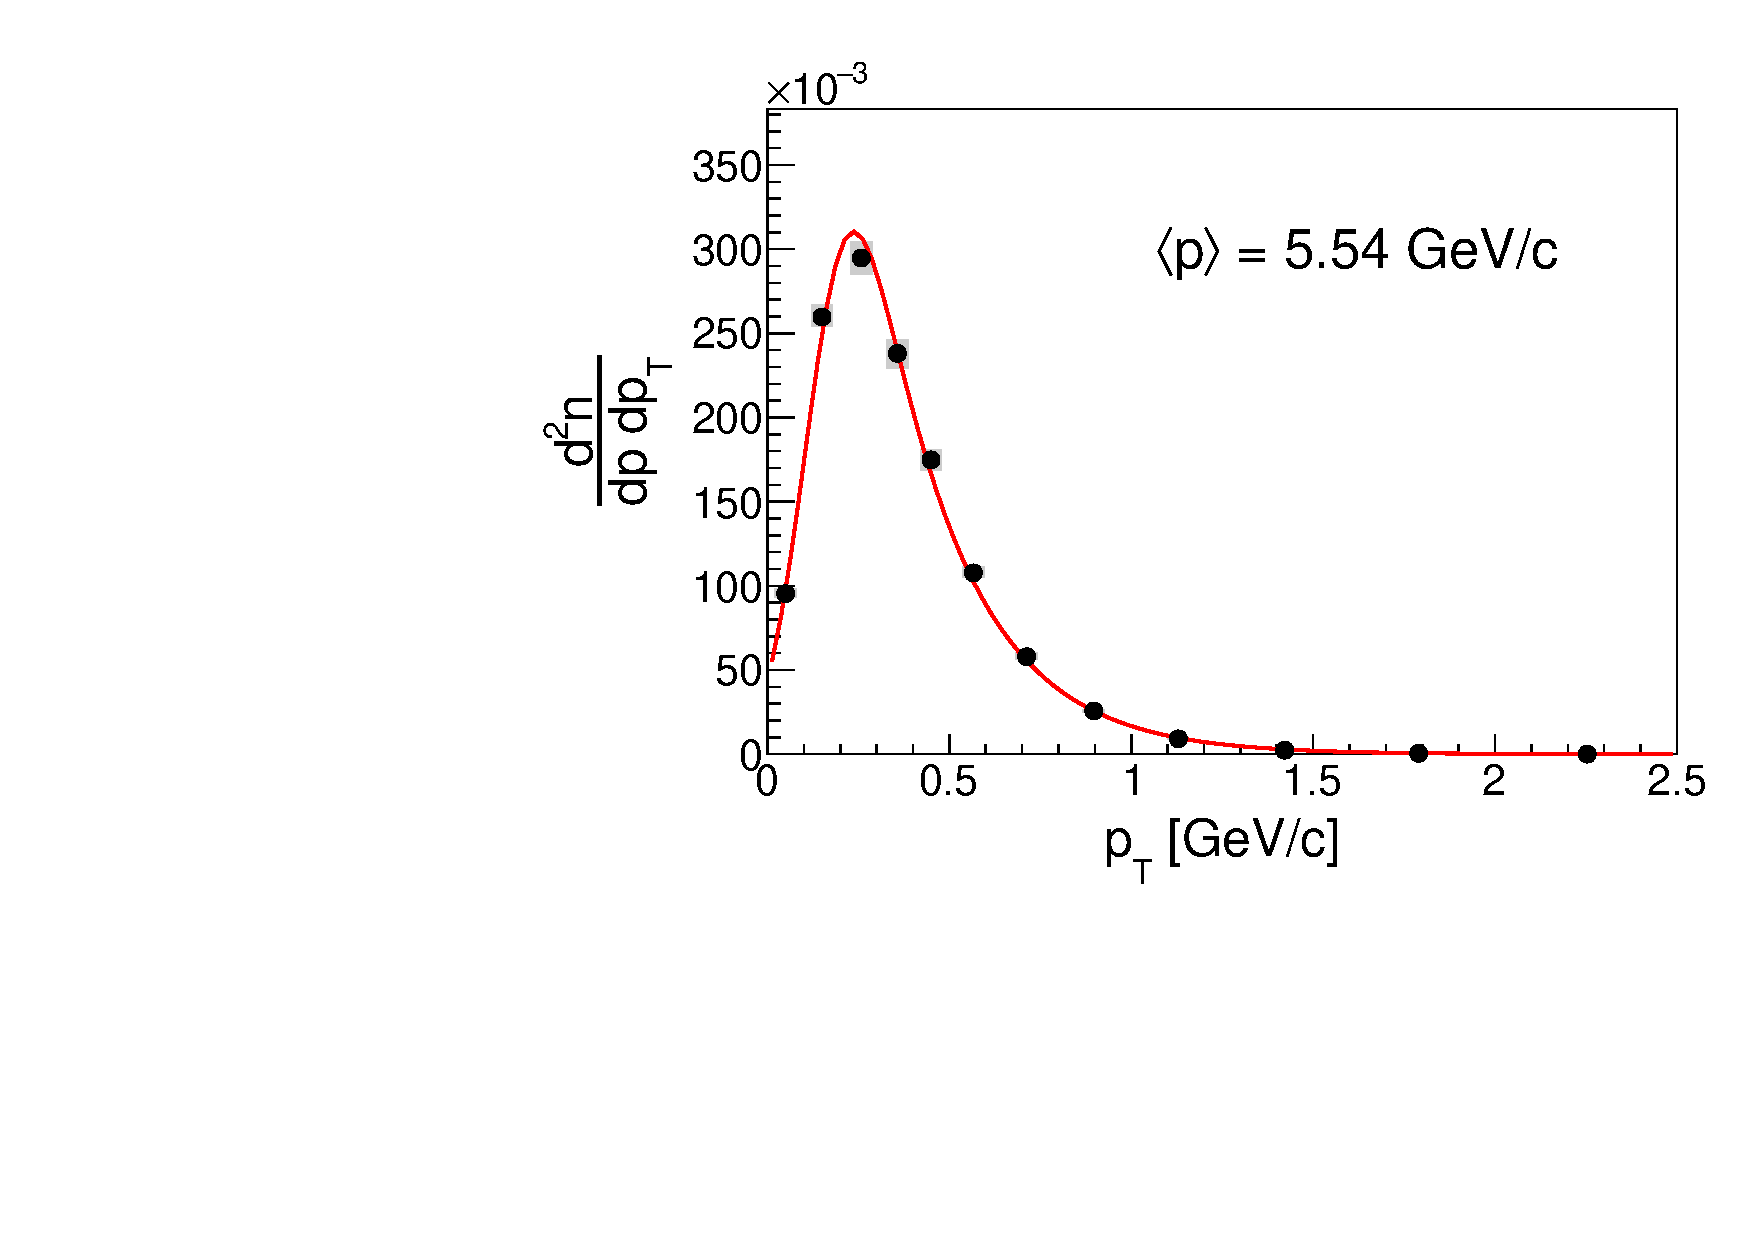
\includegraphics[clip, rviewport=0 0 1 1,width=0.24\textwidth]{spec/spec_pt_158_c0_p1_x18}
  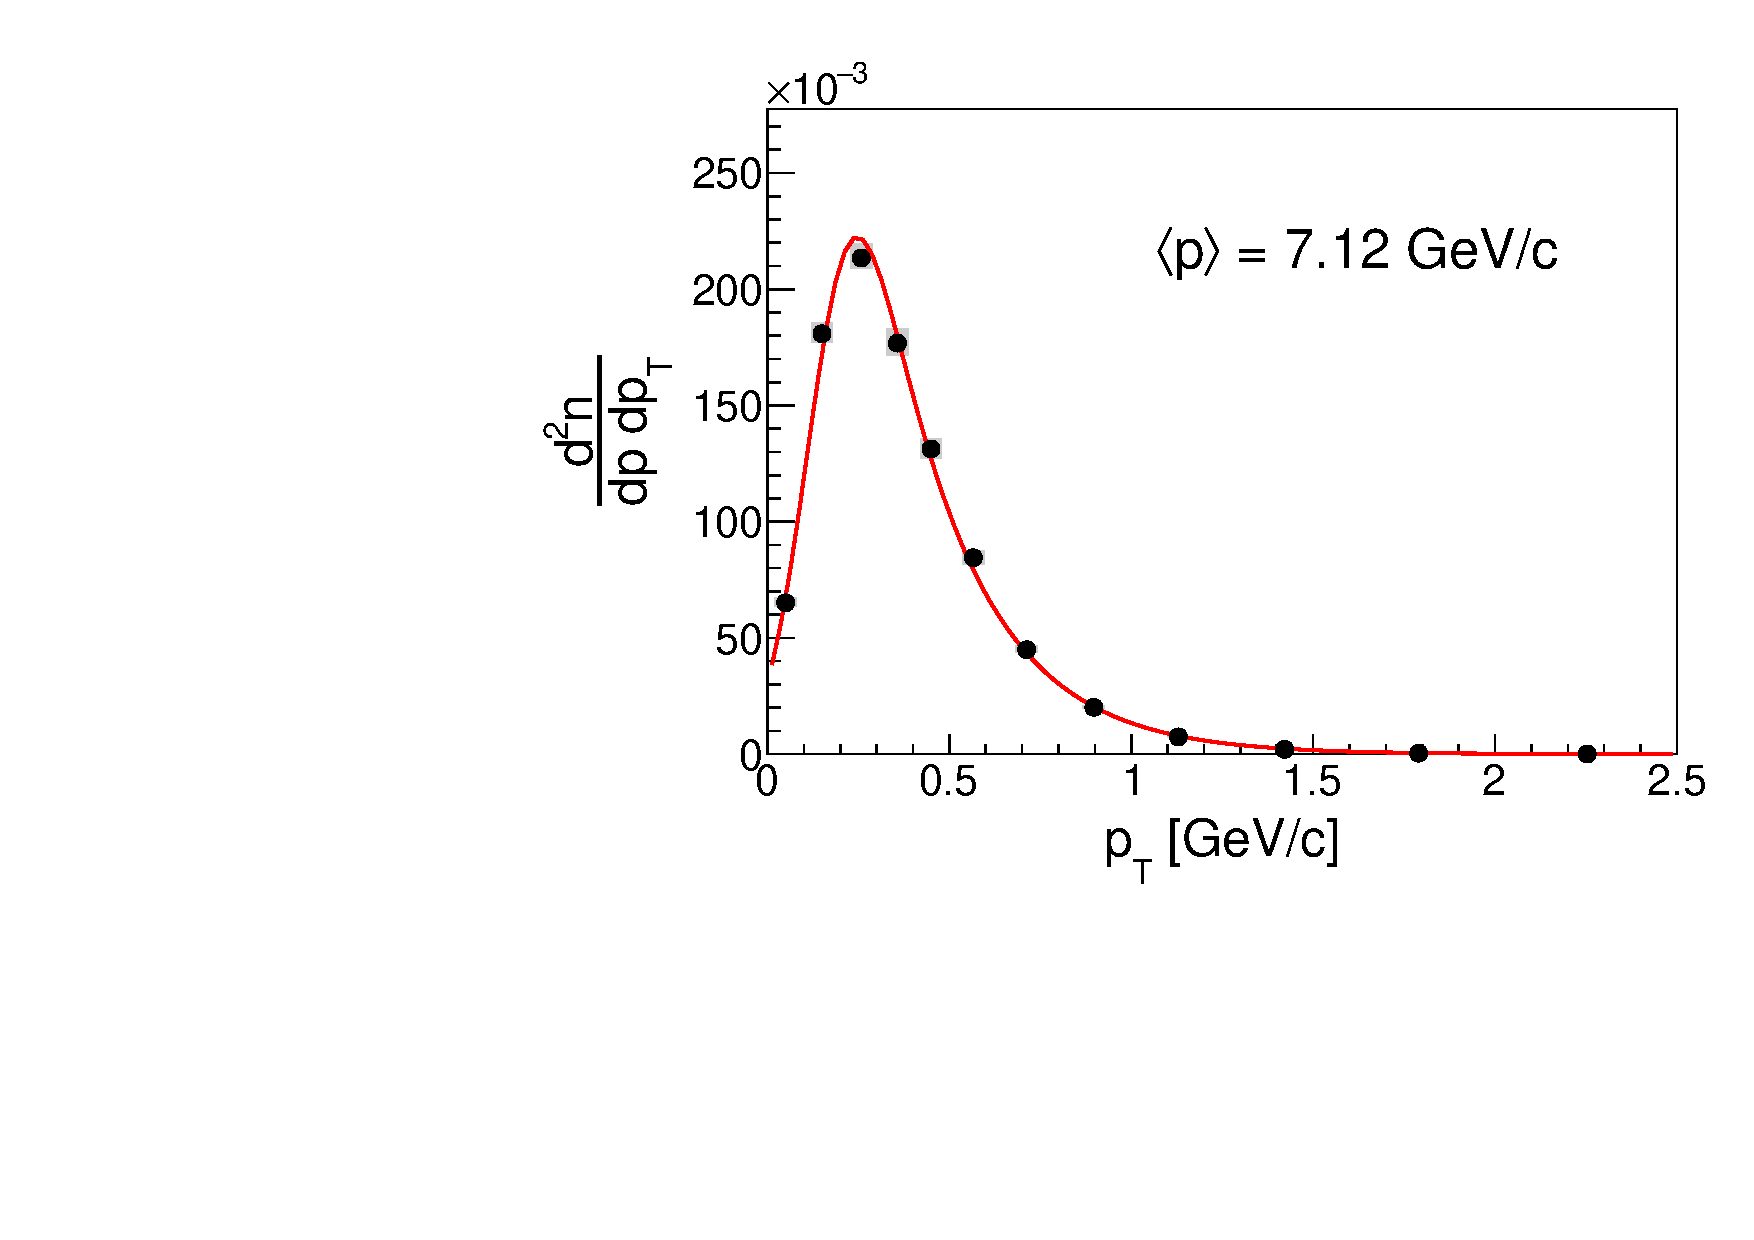
\includegraphics[clip, rviewport=0 0 1 1,width=0.24\textwidth]{spec/spec_pt_158_c0_p1_x19}
  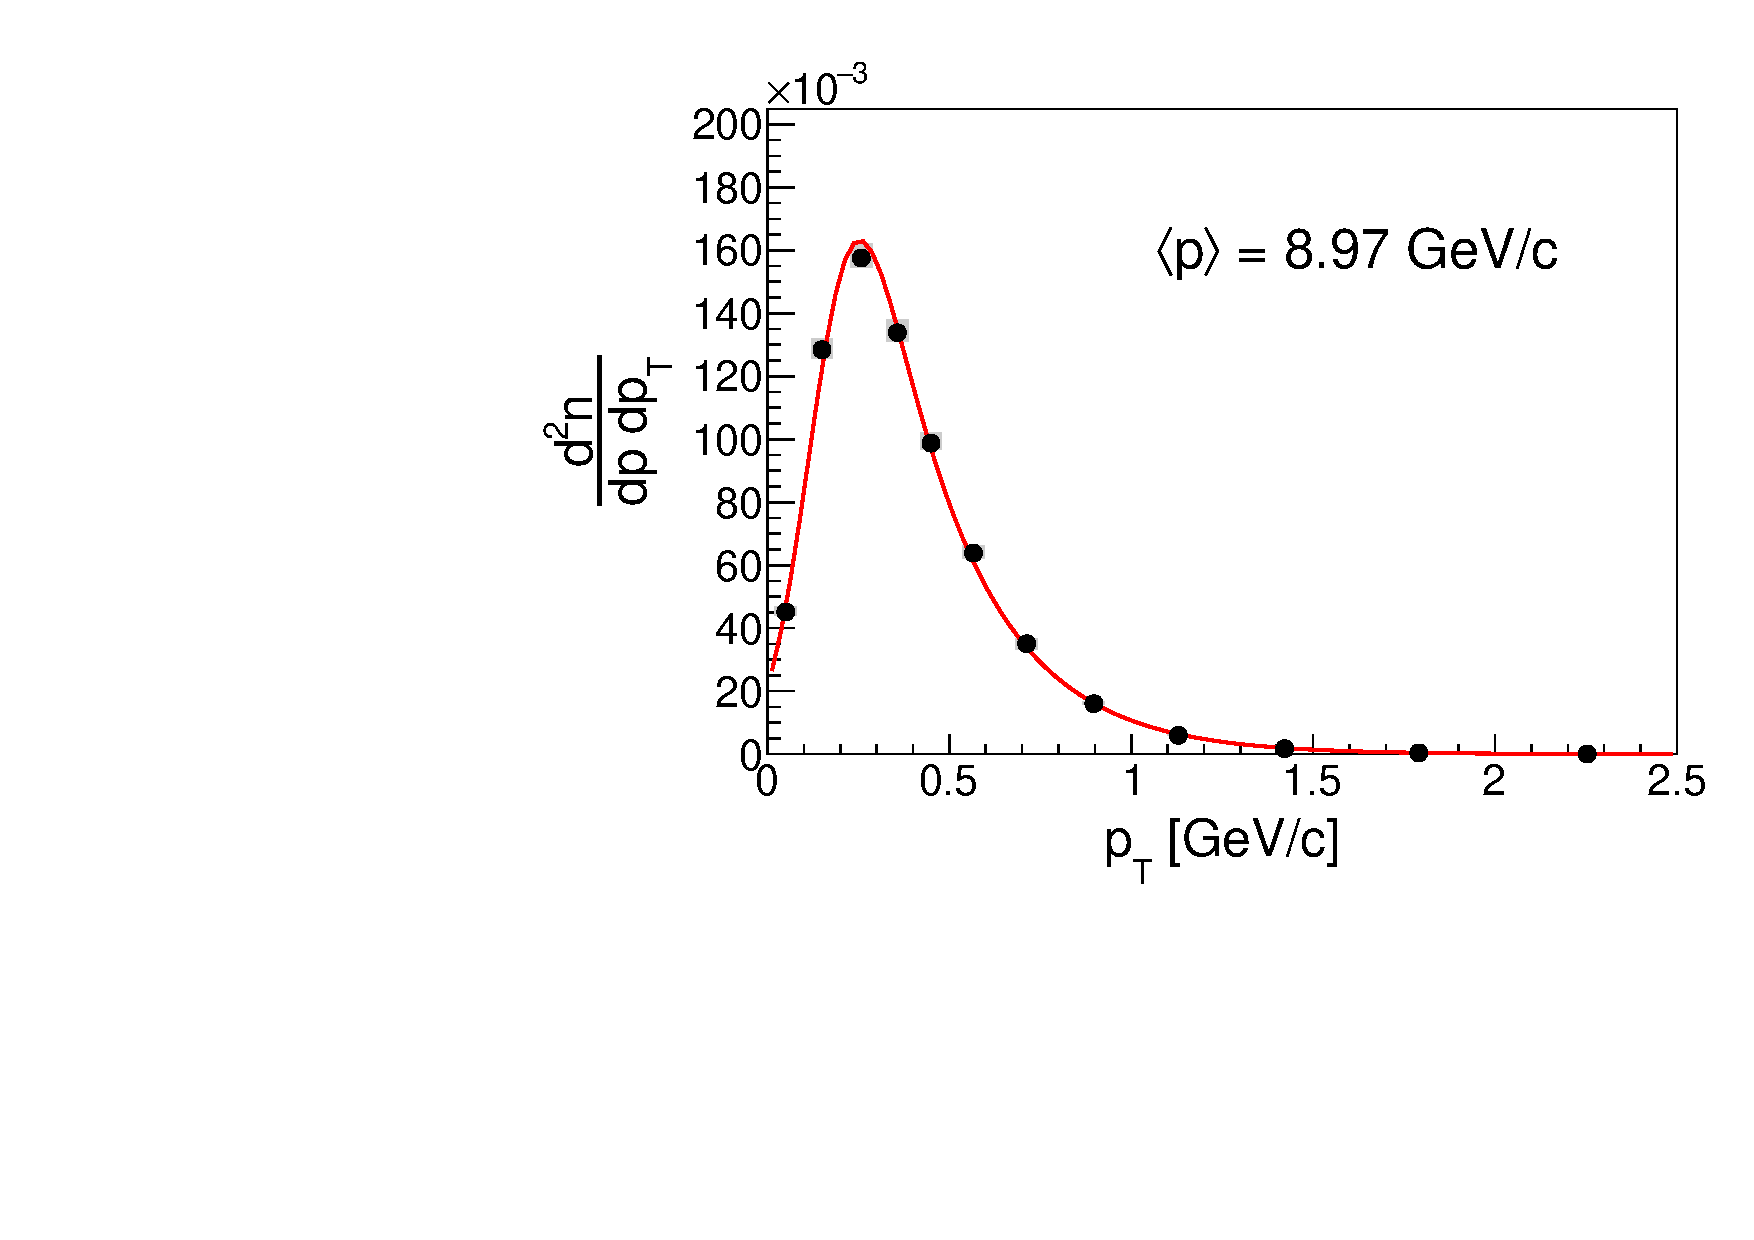
\includegraphics[clip, rviewport=0 0 1 1,width=0.24\textwidth]{spec/spec_pt_158_c0_p1_x20}

  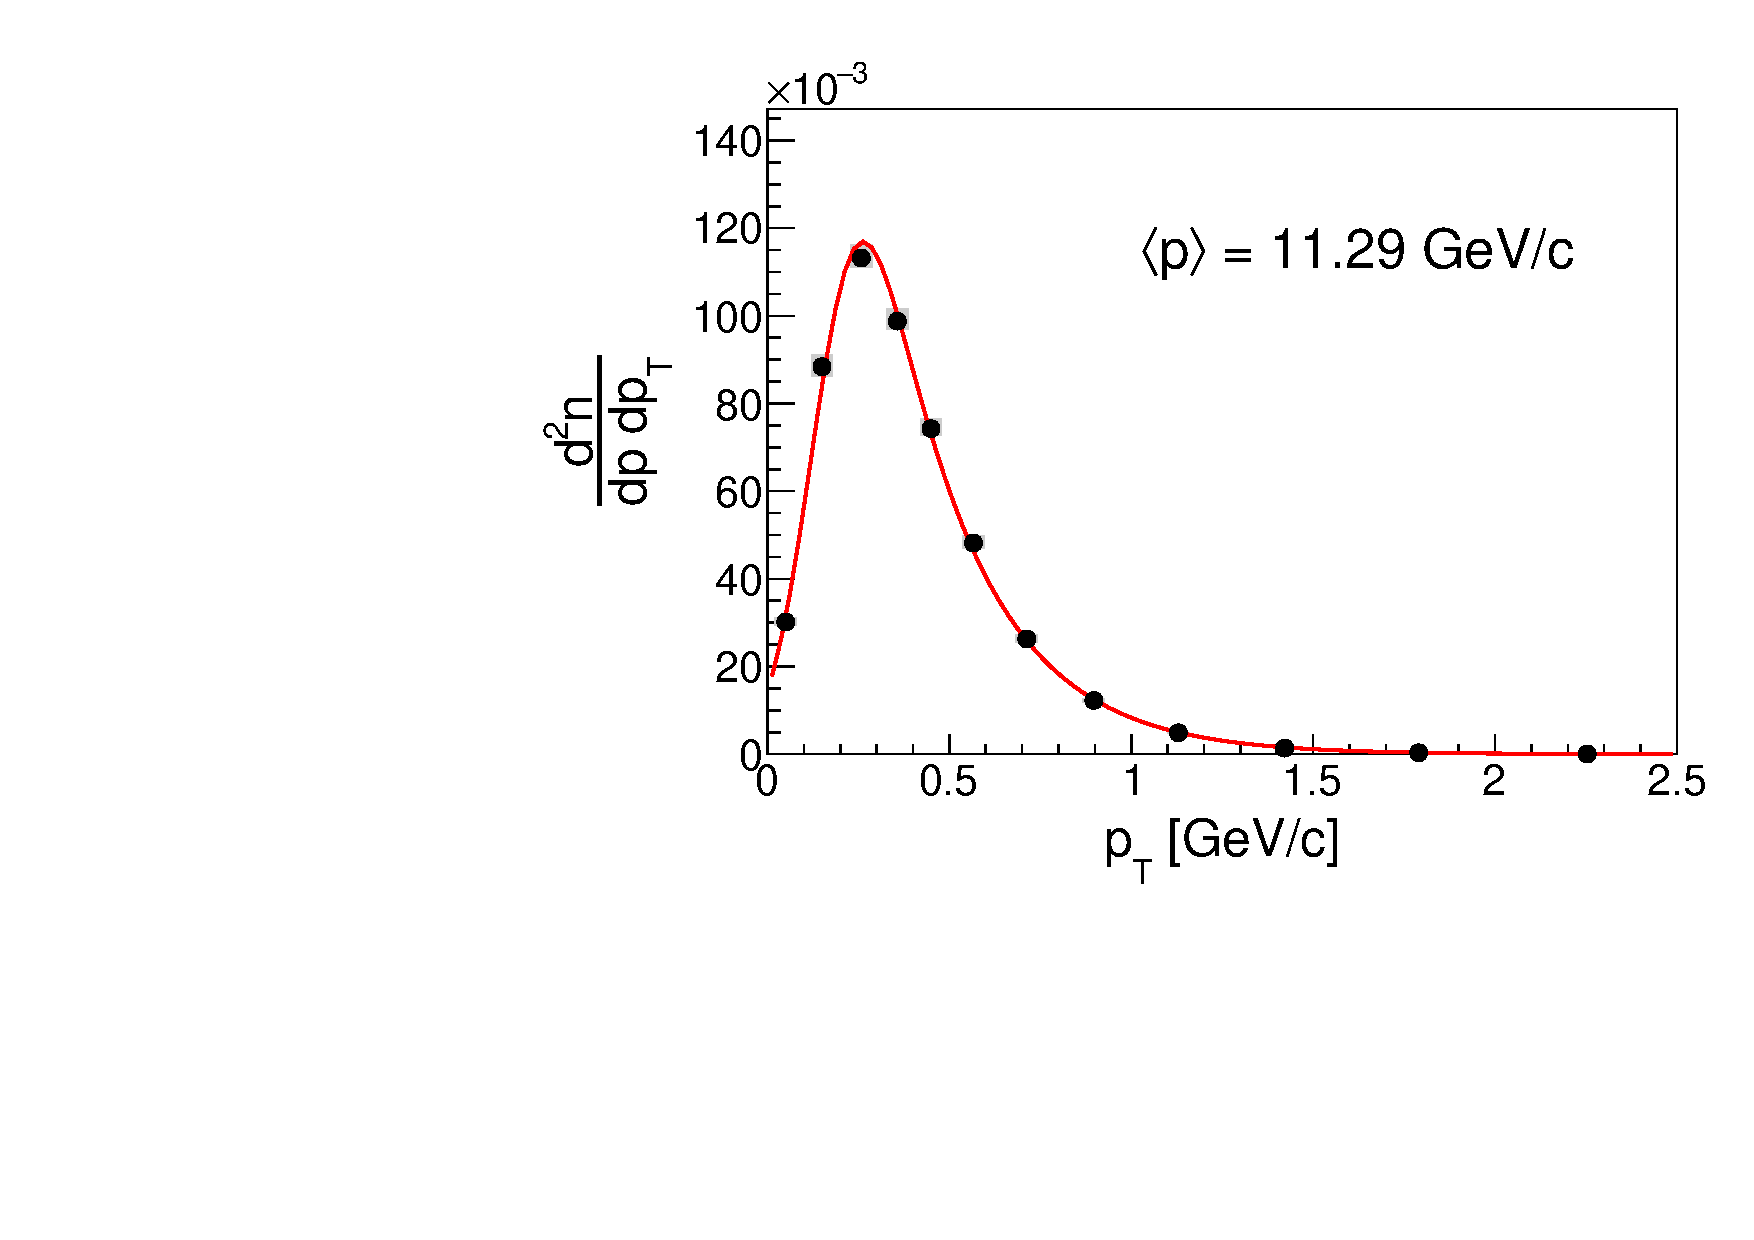
\includegraphics[clip, rviewport=0 0 1 1,width=0.24\textwidth]{spec/spec_pt_158_c0_p1_x21}
  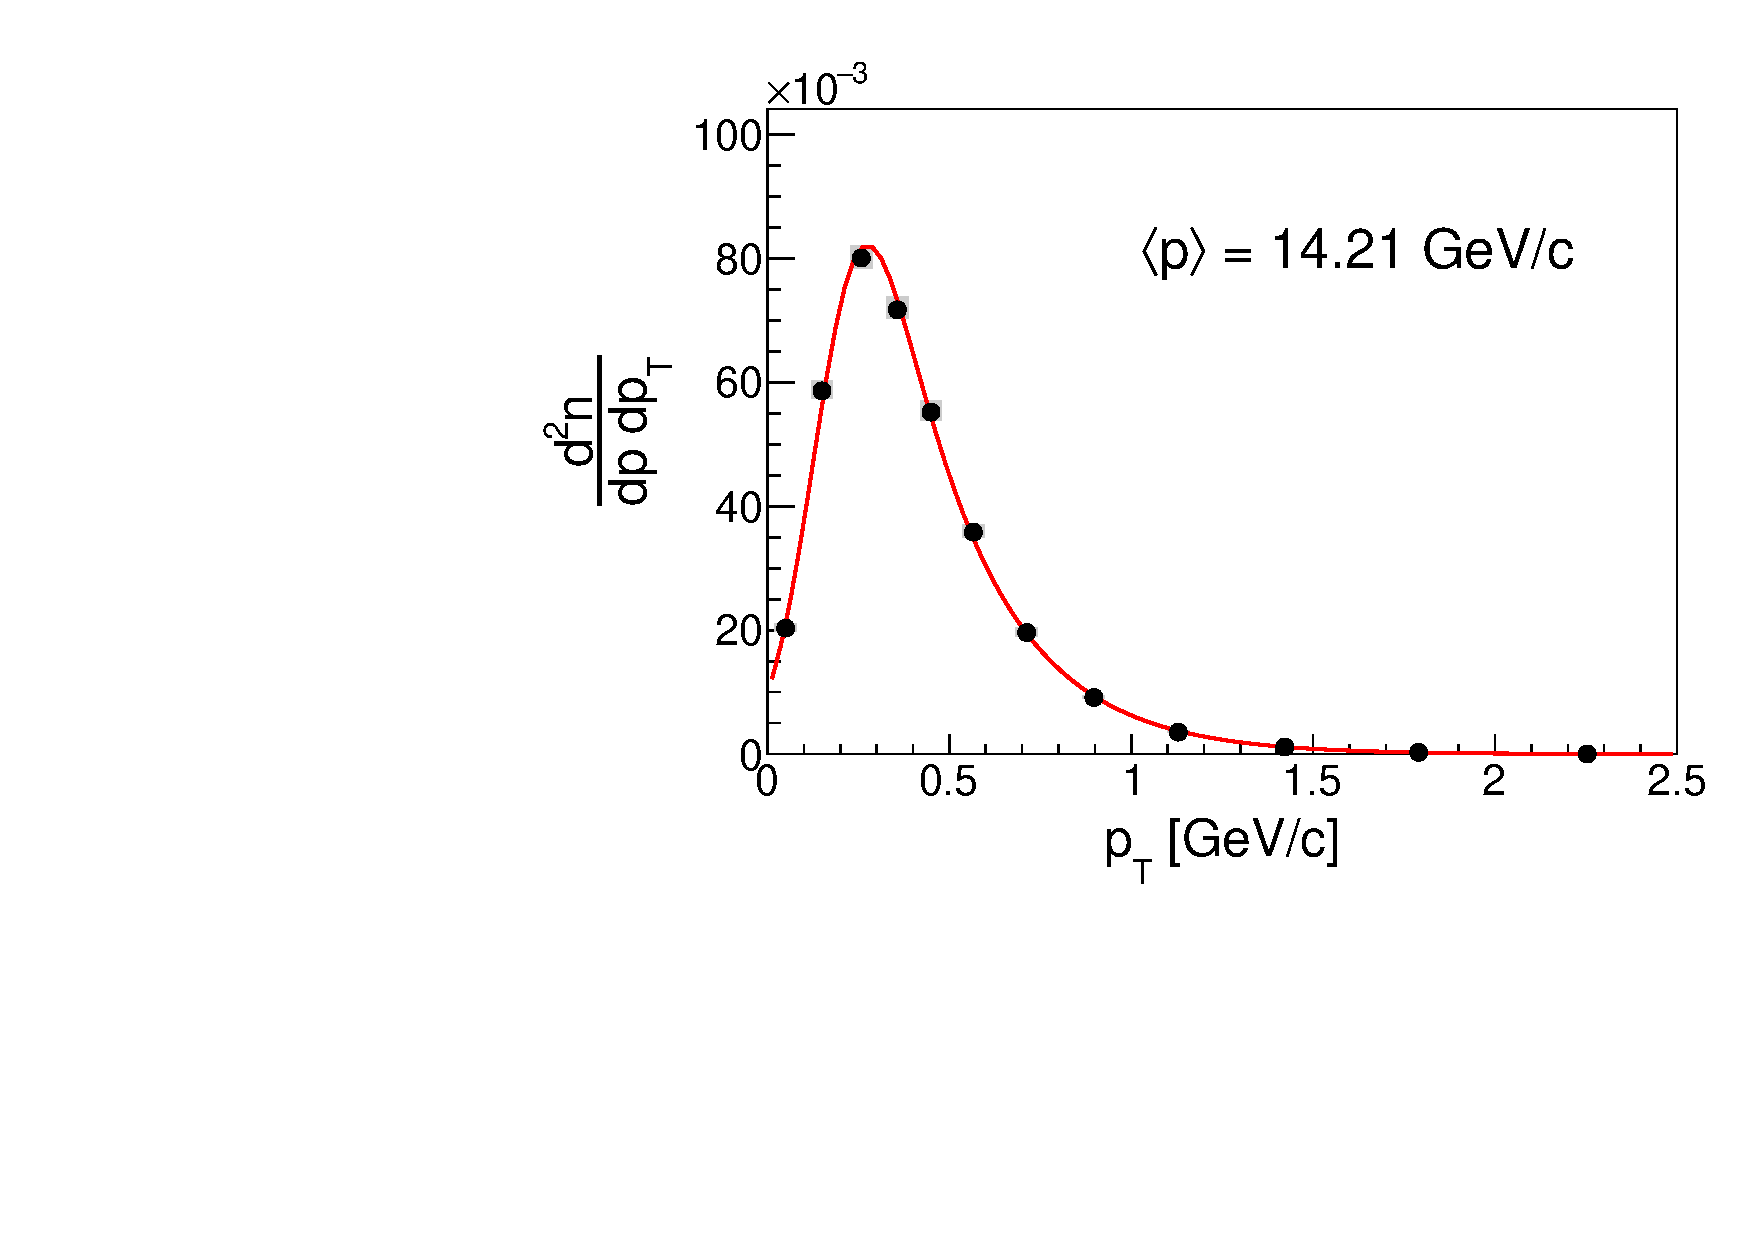
\includegraphics[clip, rviewport=0 0 1 1,width=0.24\textwidth]{spec/spec_pt_158_c0_p1_x22}
  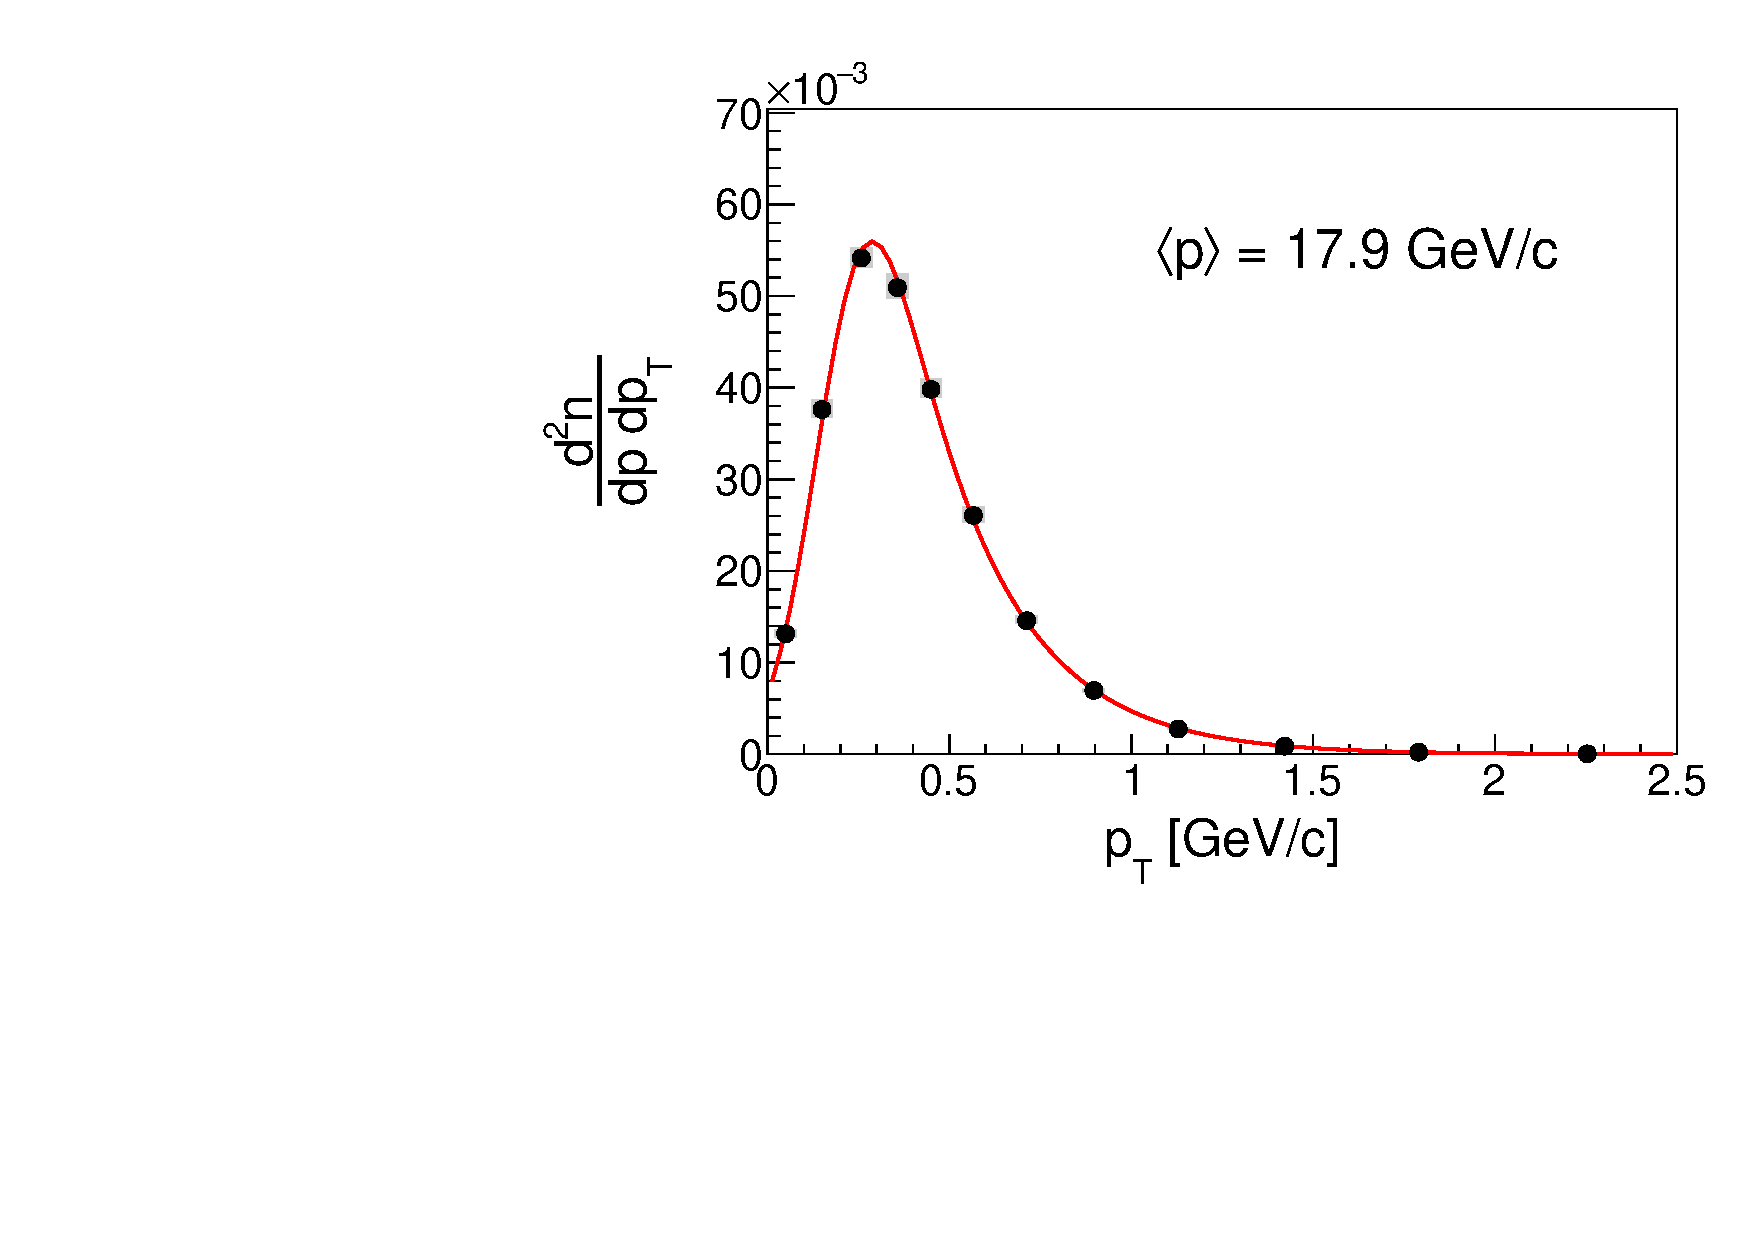
\includegraphics[clip, rviewport=0 0 1 1,width=0.24\textwidth]{spec/spec_pt_158_c0_p1_x23}
  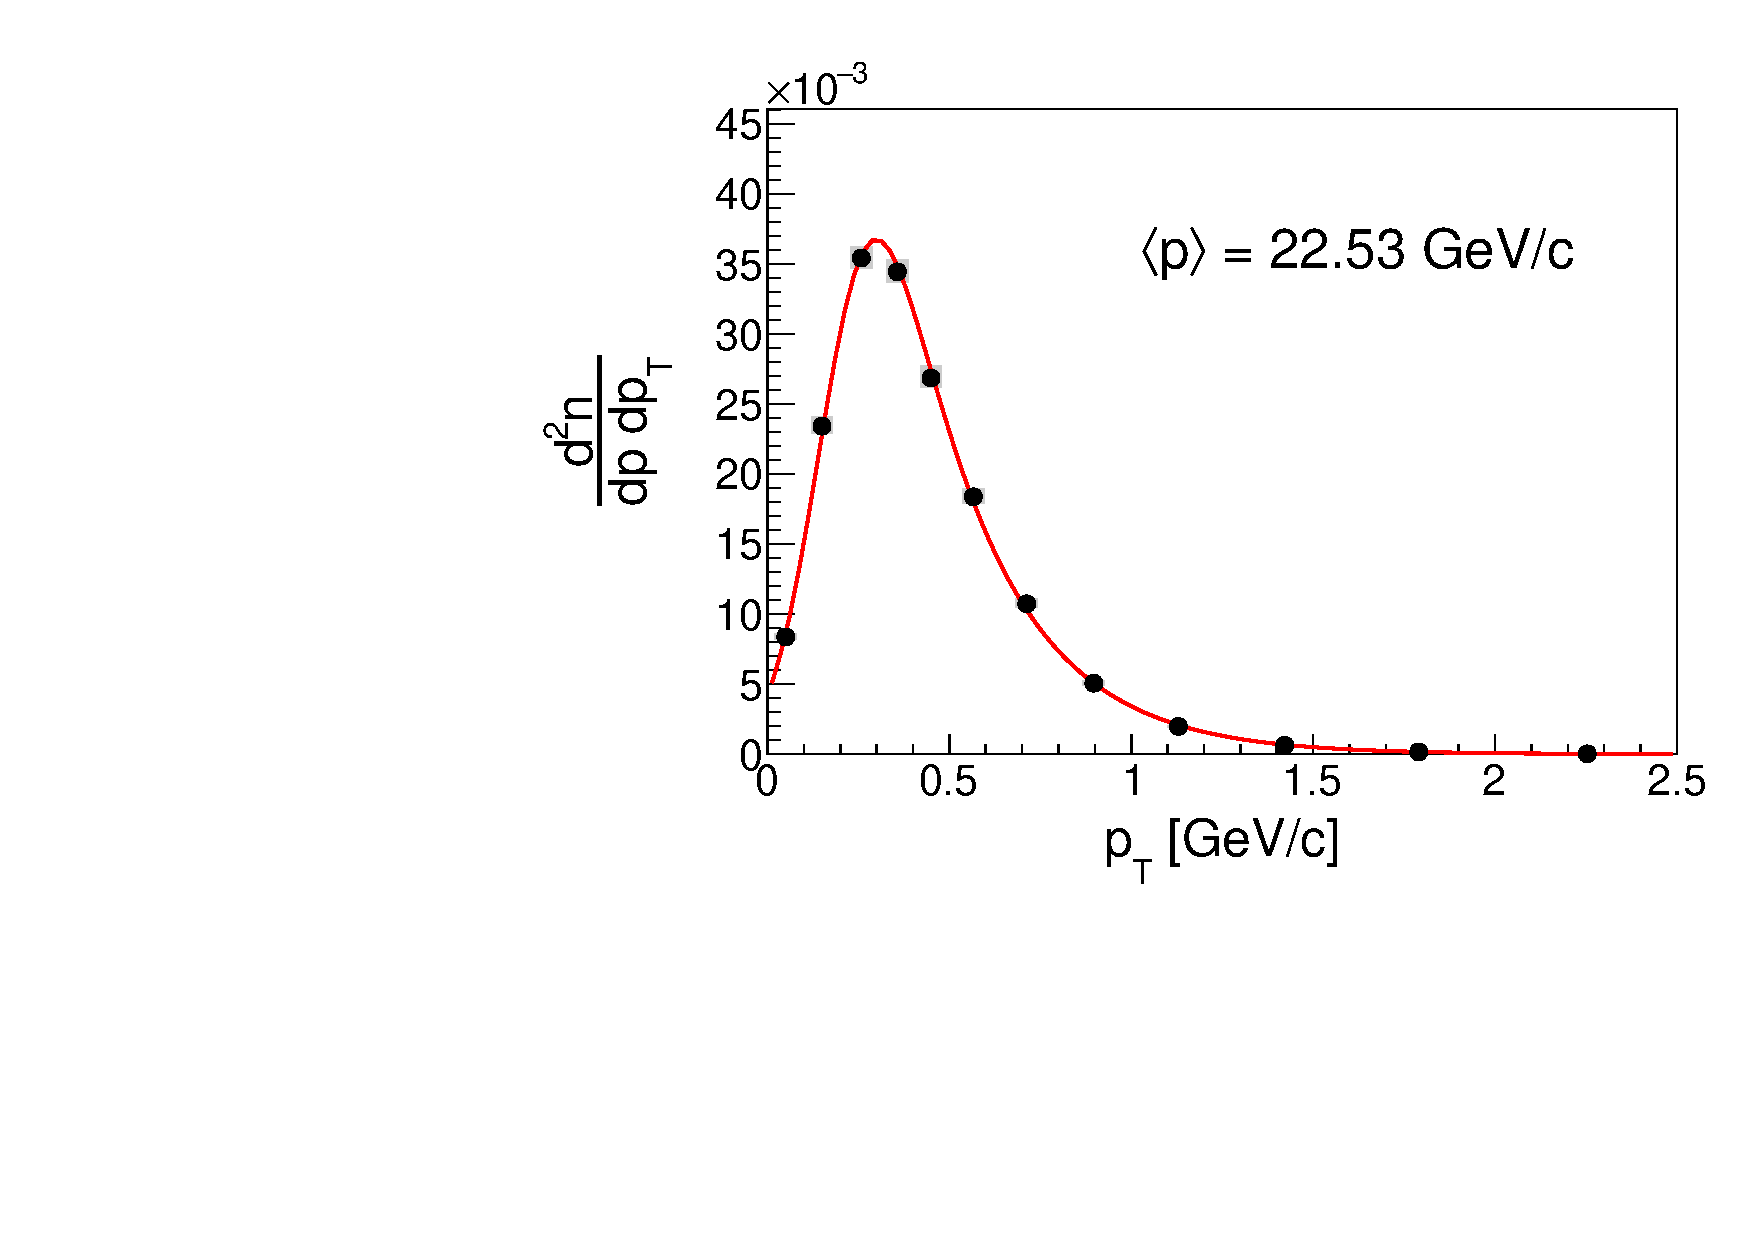
\includegraphics[clip, rviewport=0 0 1 1,width=0.24\textwidth]{spec/spec_pt_158_c0_p1_x24}

  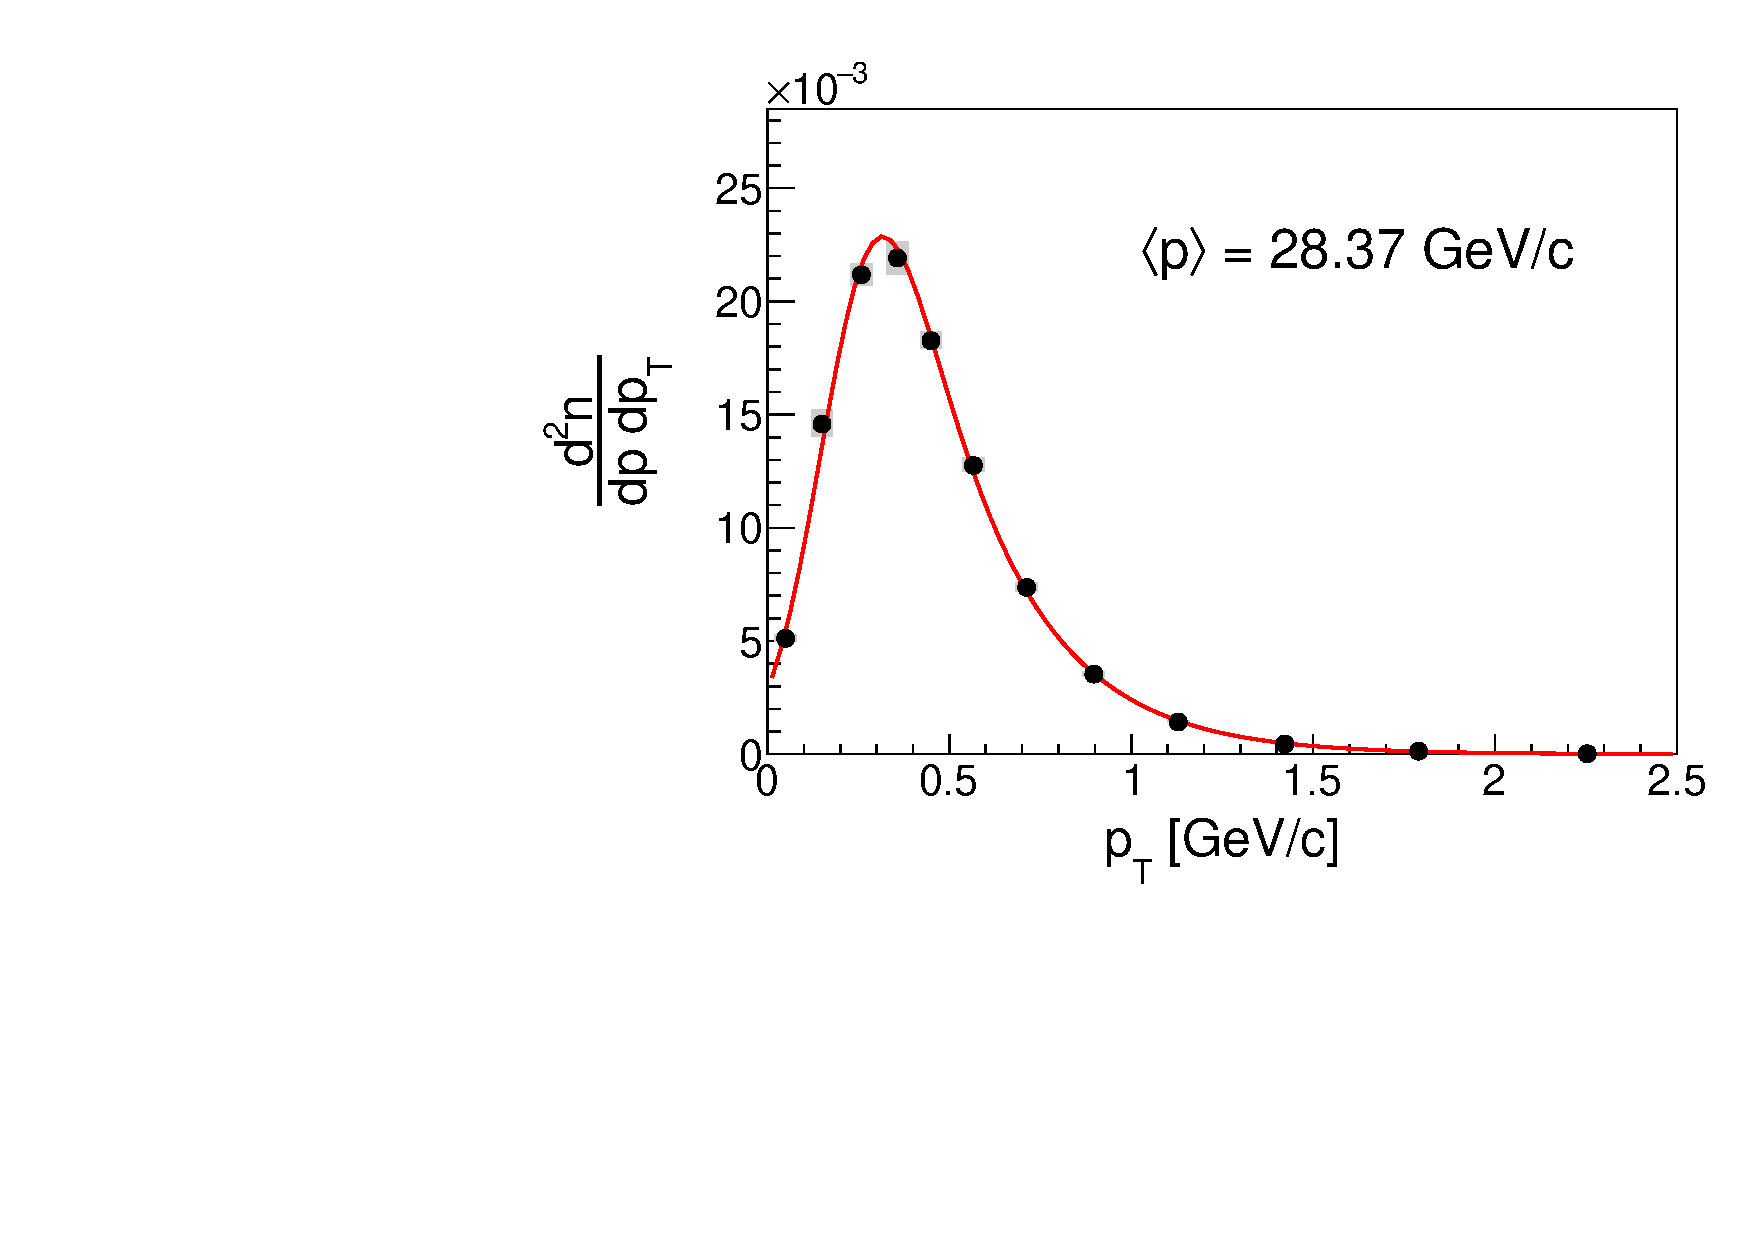
\includegraphics[clip, rviewport=0 0 1 1,width=0.24\textwidth]{spec/spec_pt_158_c0_p1_x25}
  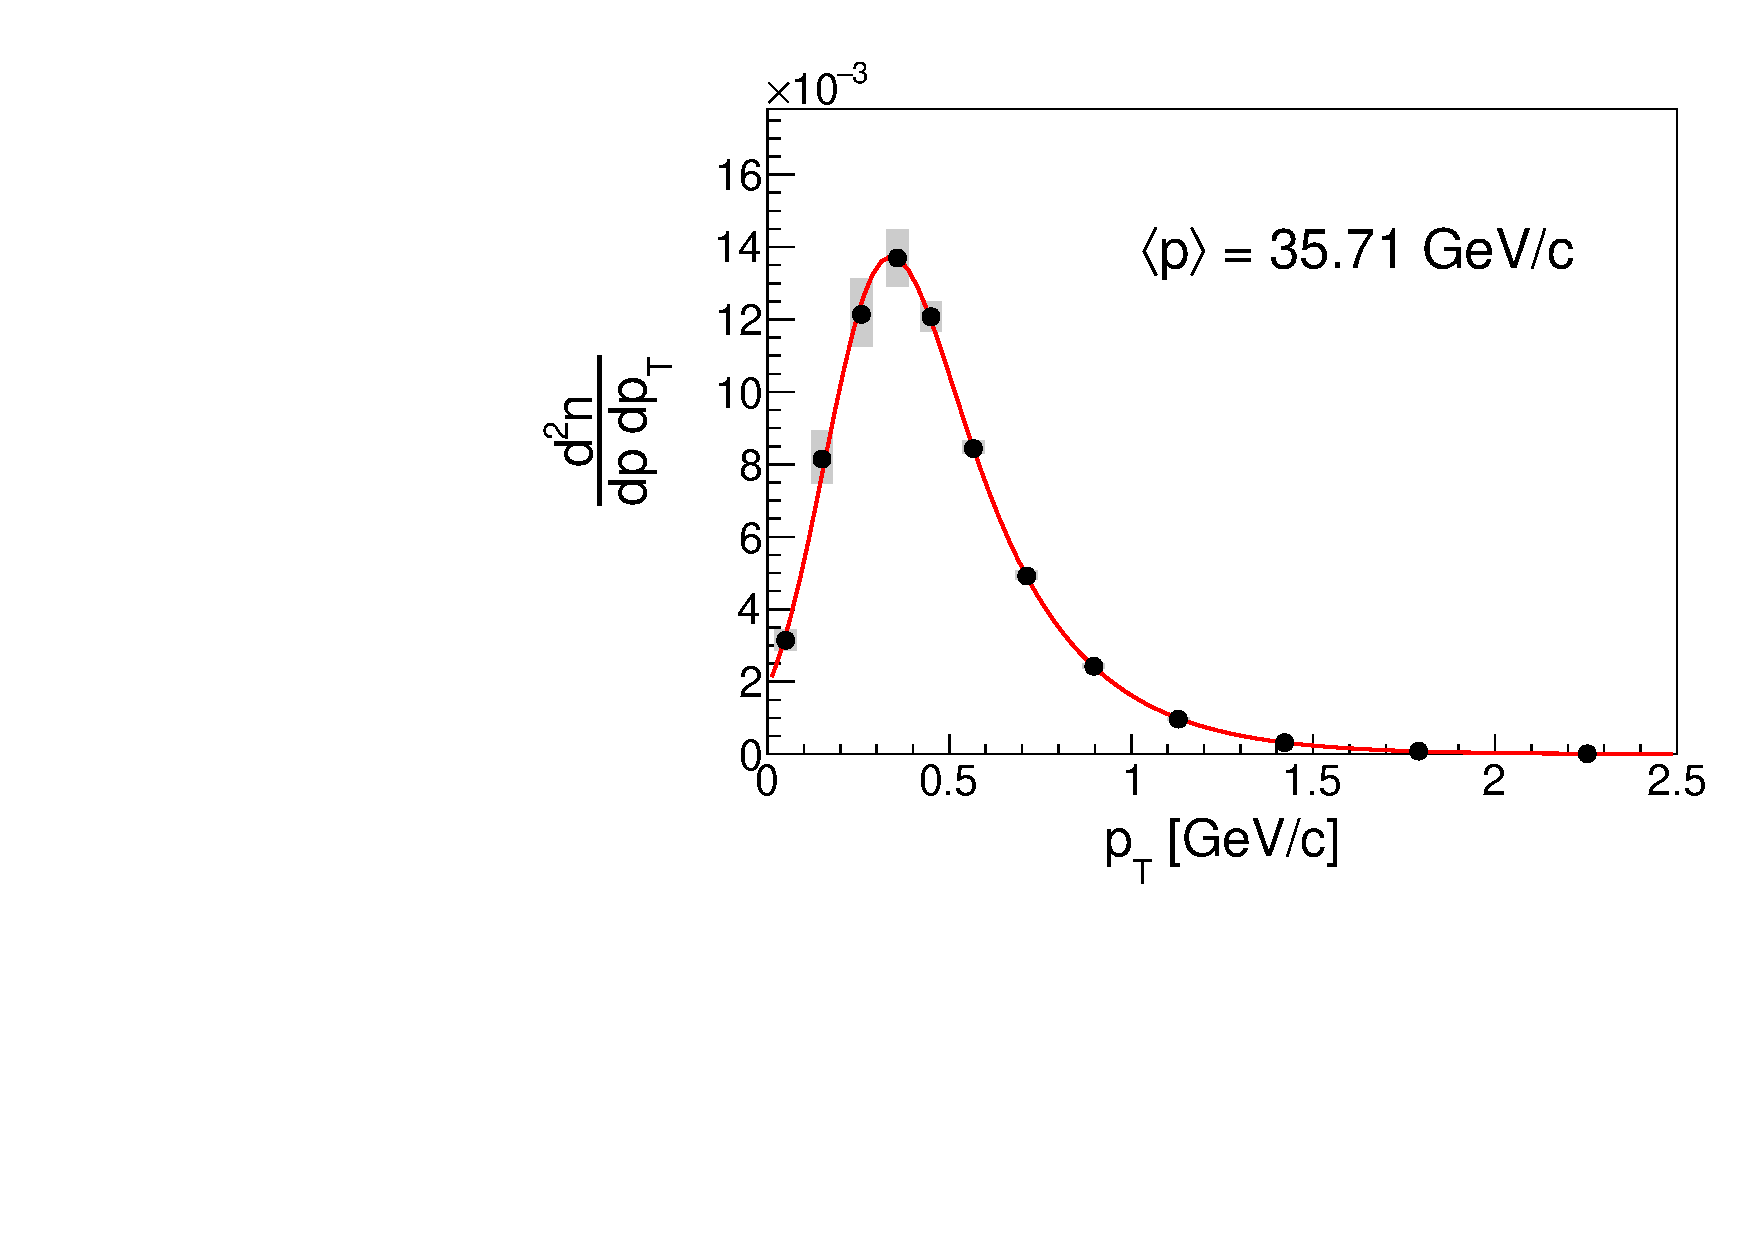
\includegraphics[clip, rviewport=0 0 1 1,width=0.24\textwidth]{spec/spec_pt_158_c0_p1_x26}
  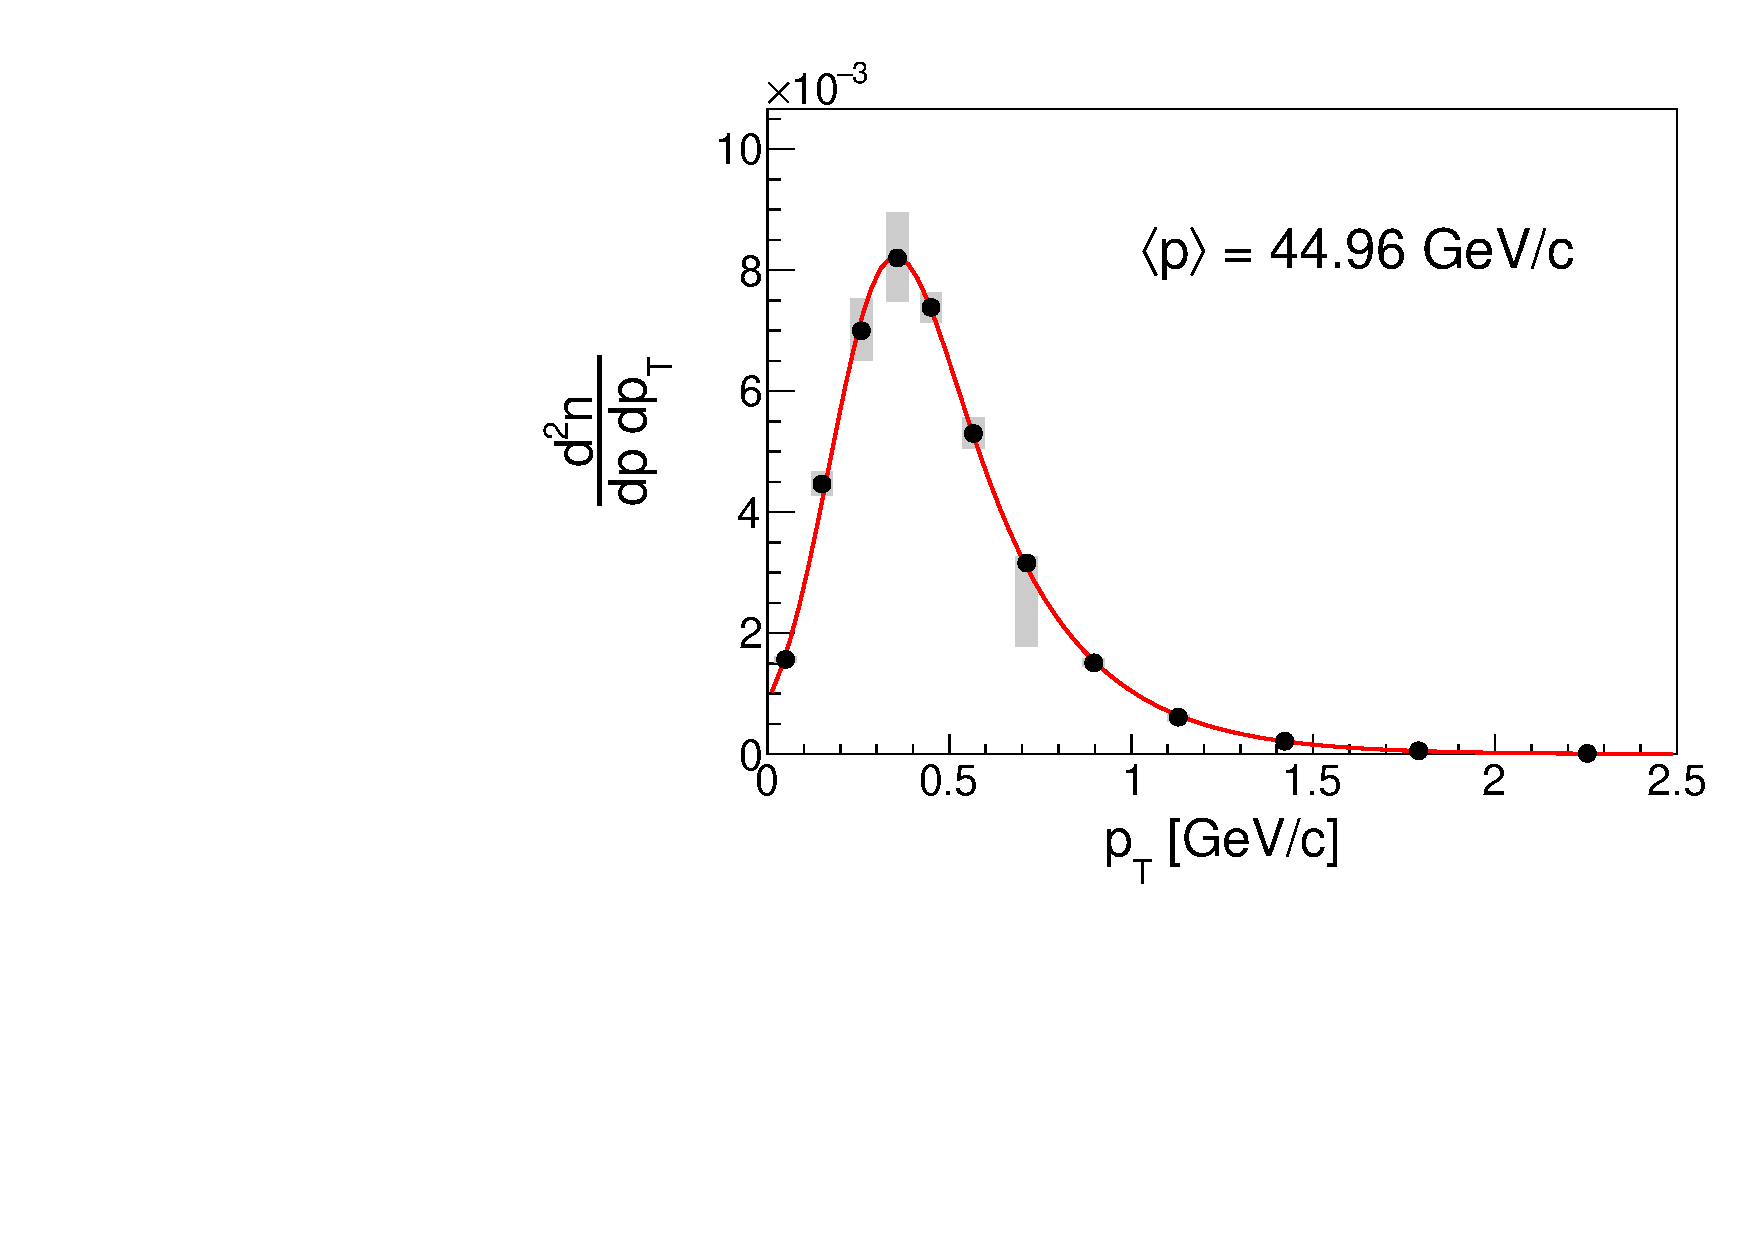
\includegraphics[clip, rviewport=0 0 1 1,width=0.24\textwidth]{spec/spec_pt_158_c0_p1_x27}
  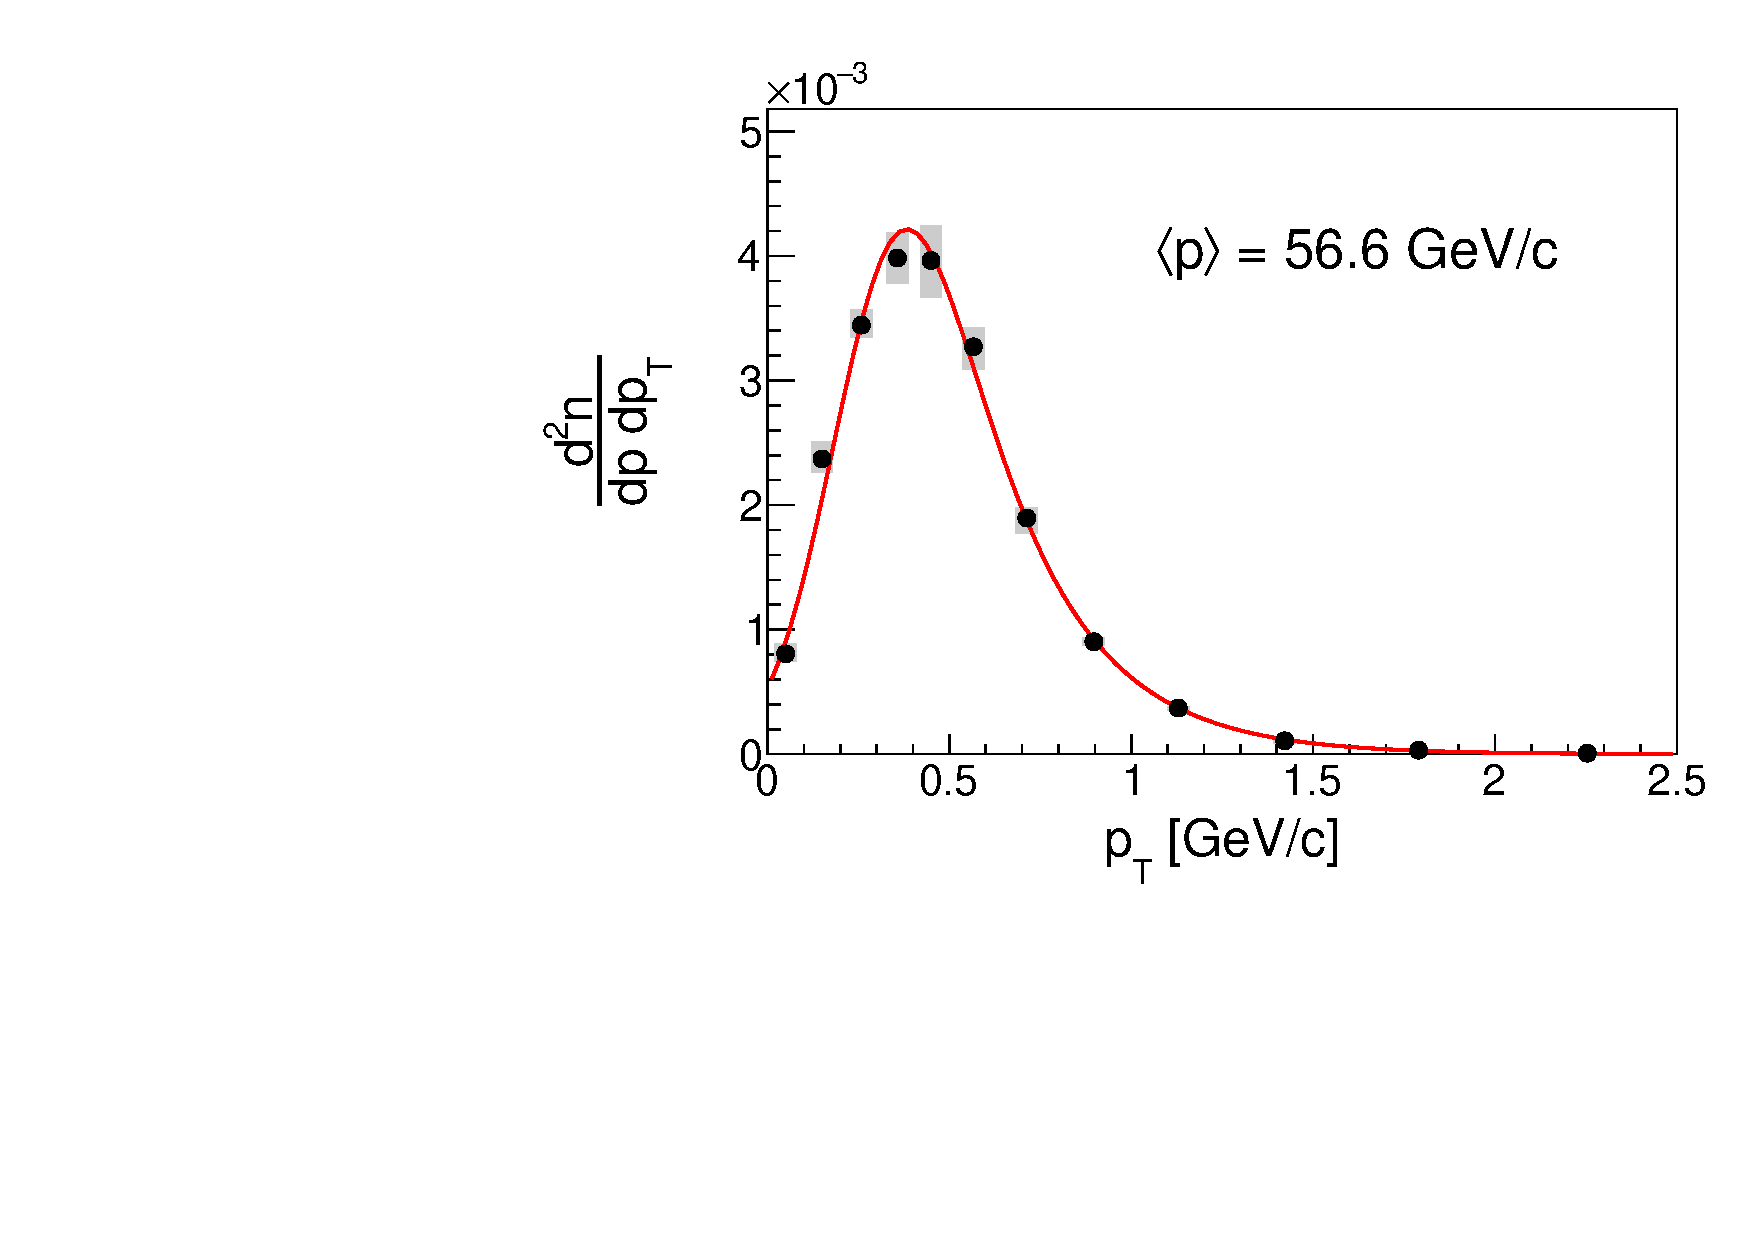
\includegraphics[clip, rviewport=0 0 1 1,width=0.24\textwidth]{spec/spec_pt_158_c0_p1_x28}

  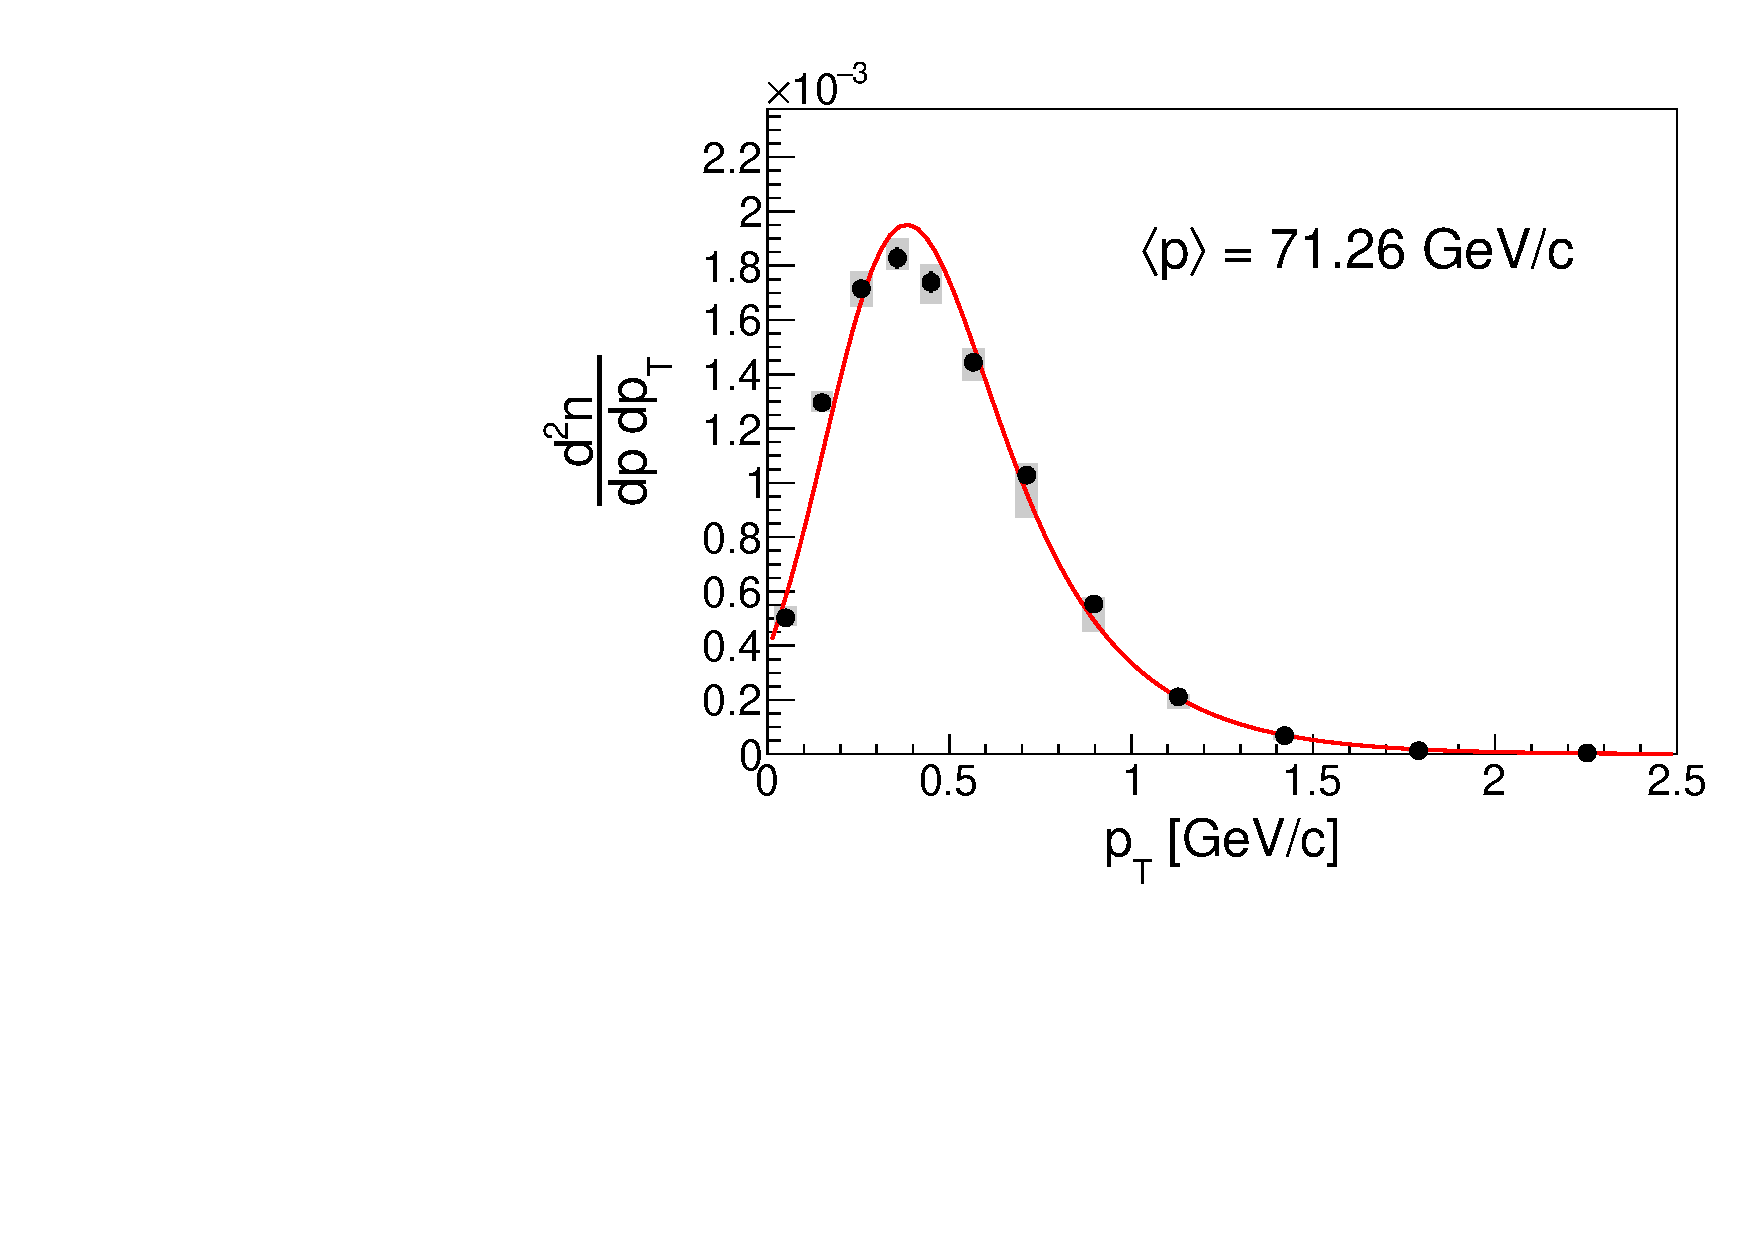
\includegraphics[clip, rviewport=0 0 1 1,width=0.24\textwidth]{spec/spec_pt_158_c0_p1_x29}
  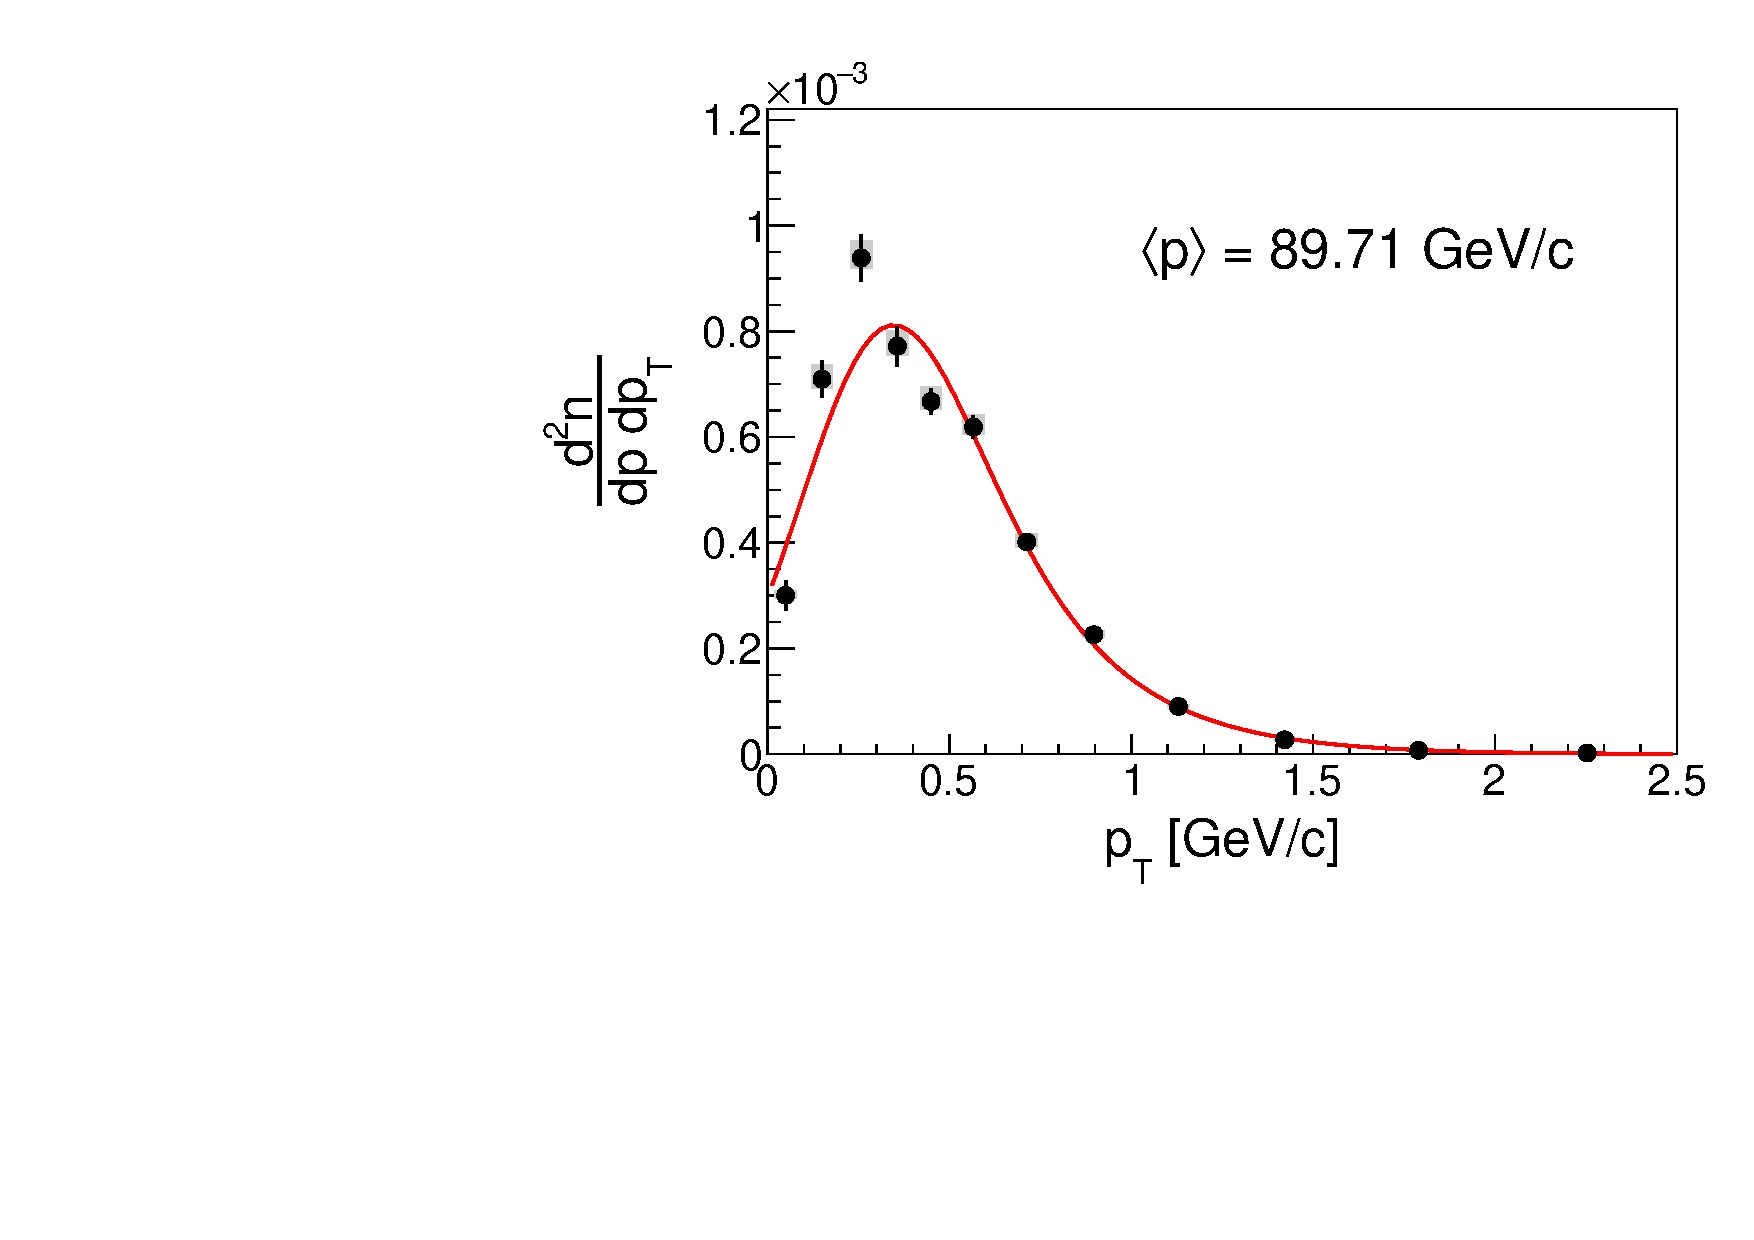
\includegraphics[clip, rviewport=0 0 1 1,width=0.24\textwidth]{spec/spec_pt_158_c0_p1_x30}
  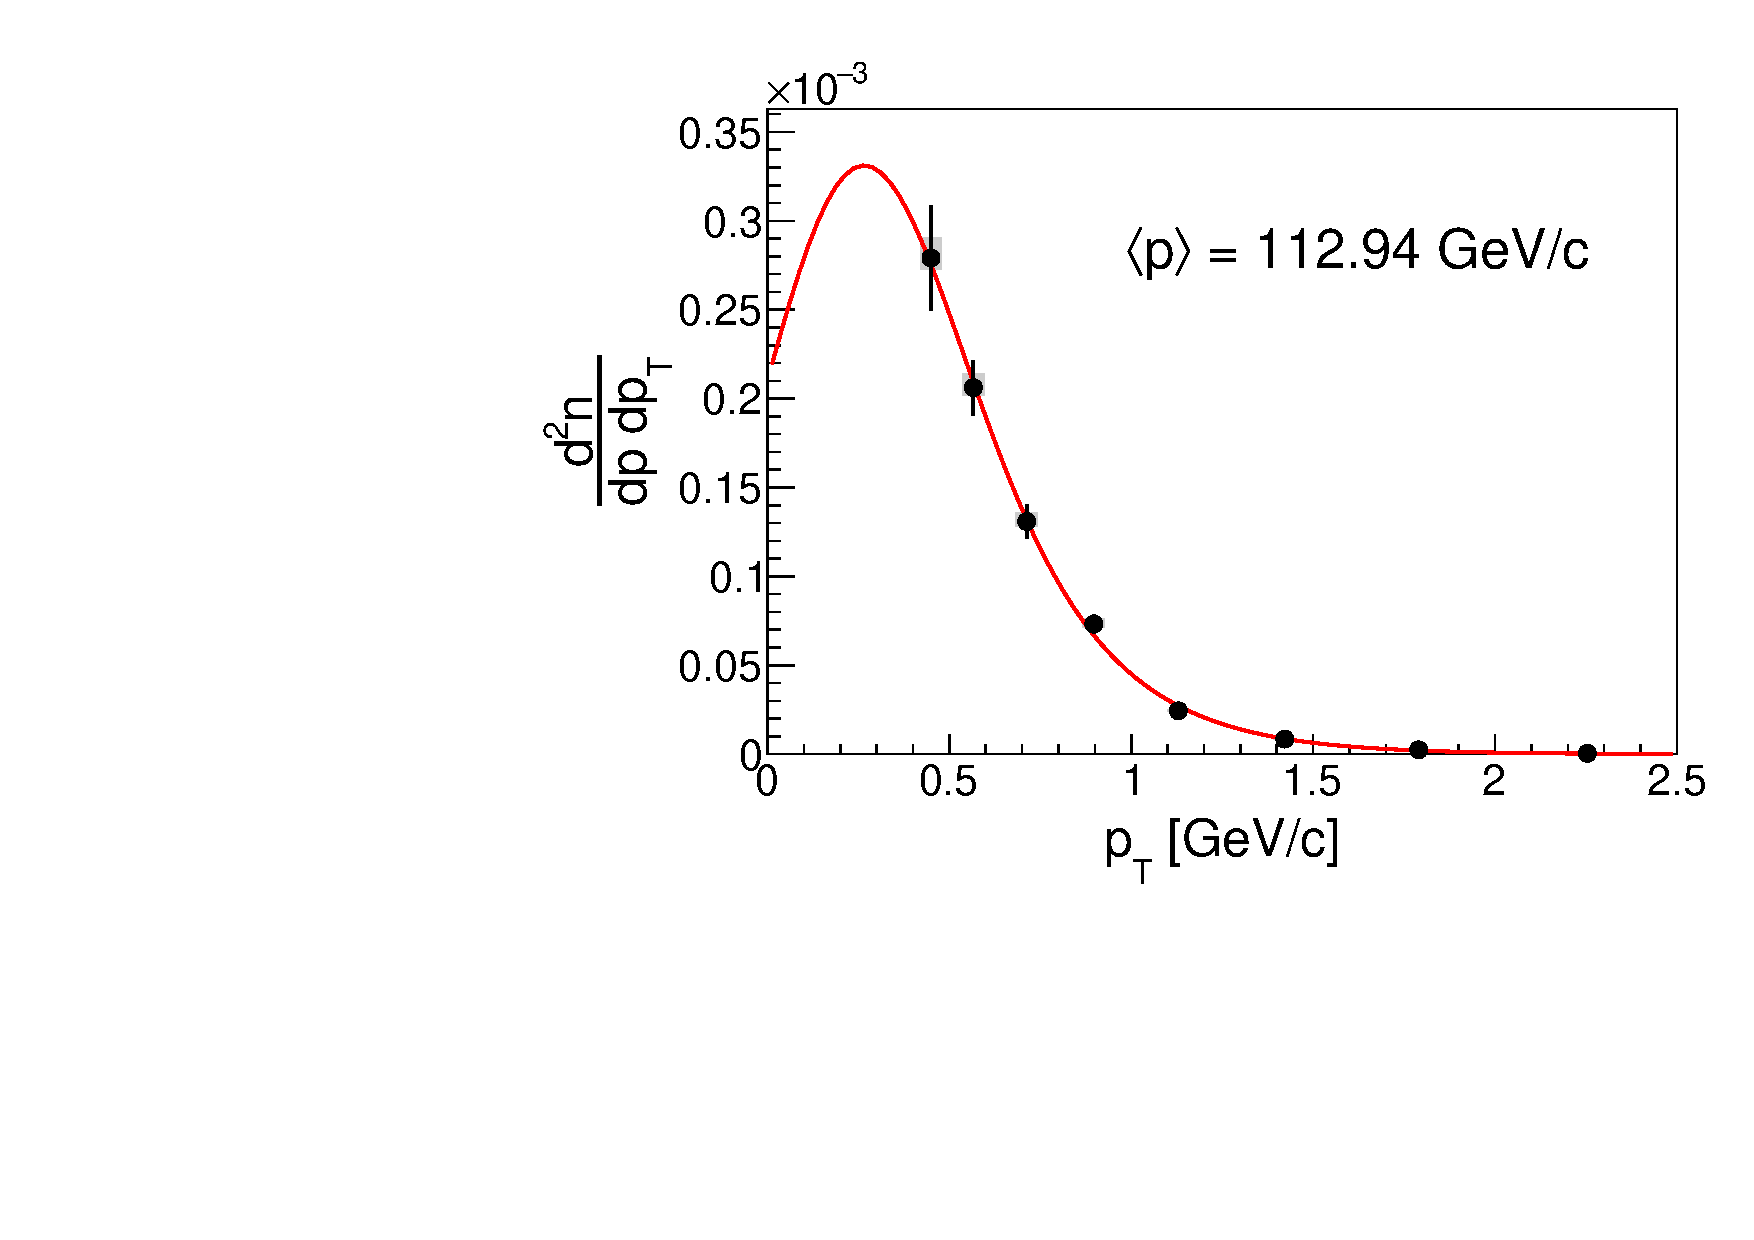
\includegraphics[clip, rviewport=0 0 1 1,width=0.24\textwidth]{spec/spec_pt_158_c0_p1_x31}

  \caption{Double-differential spectra $\frac{\text{d}^2n}{\text{d}\pp\text{d}\pT}$
    of $\pi^+$ for the 158 \GeVc data set. Each plot shows one \pp bins and the value
    of $\langle\pp\rangle$ is indicated inside it. The black lines show the statistical
    uncertainties, while the gray bands show the systematic ones.}
  \label{fig:hadron:spec:dedx:all158:c0p1}
\end{figure}

%%%%%%%%%% SPEC PT ALL DEDX %%%%%%%%%%%%%%
\begin{figure}[!ht]
  \centering

  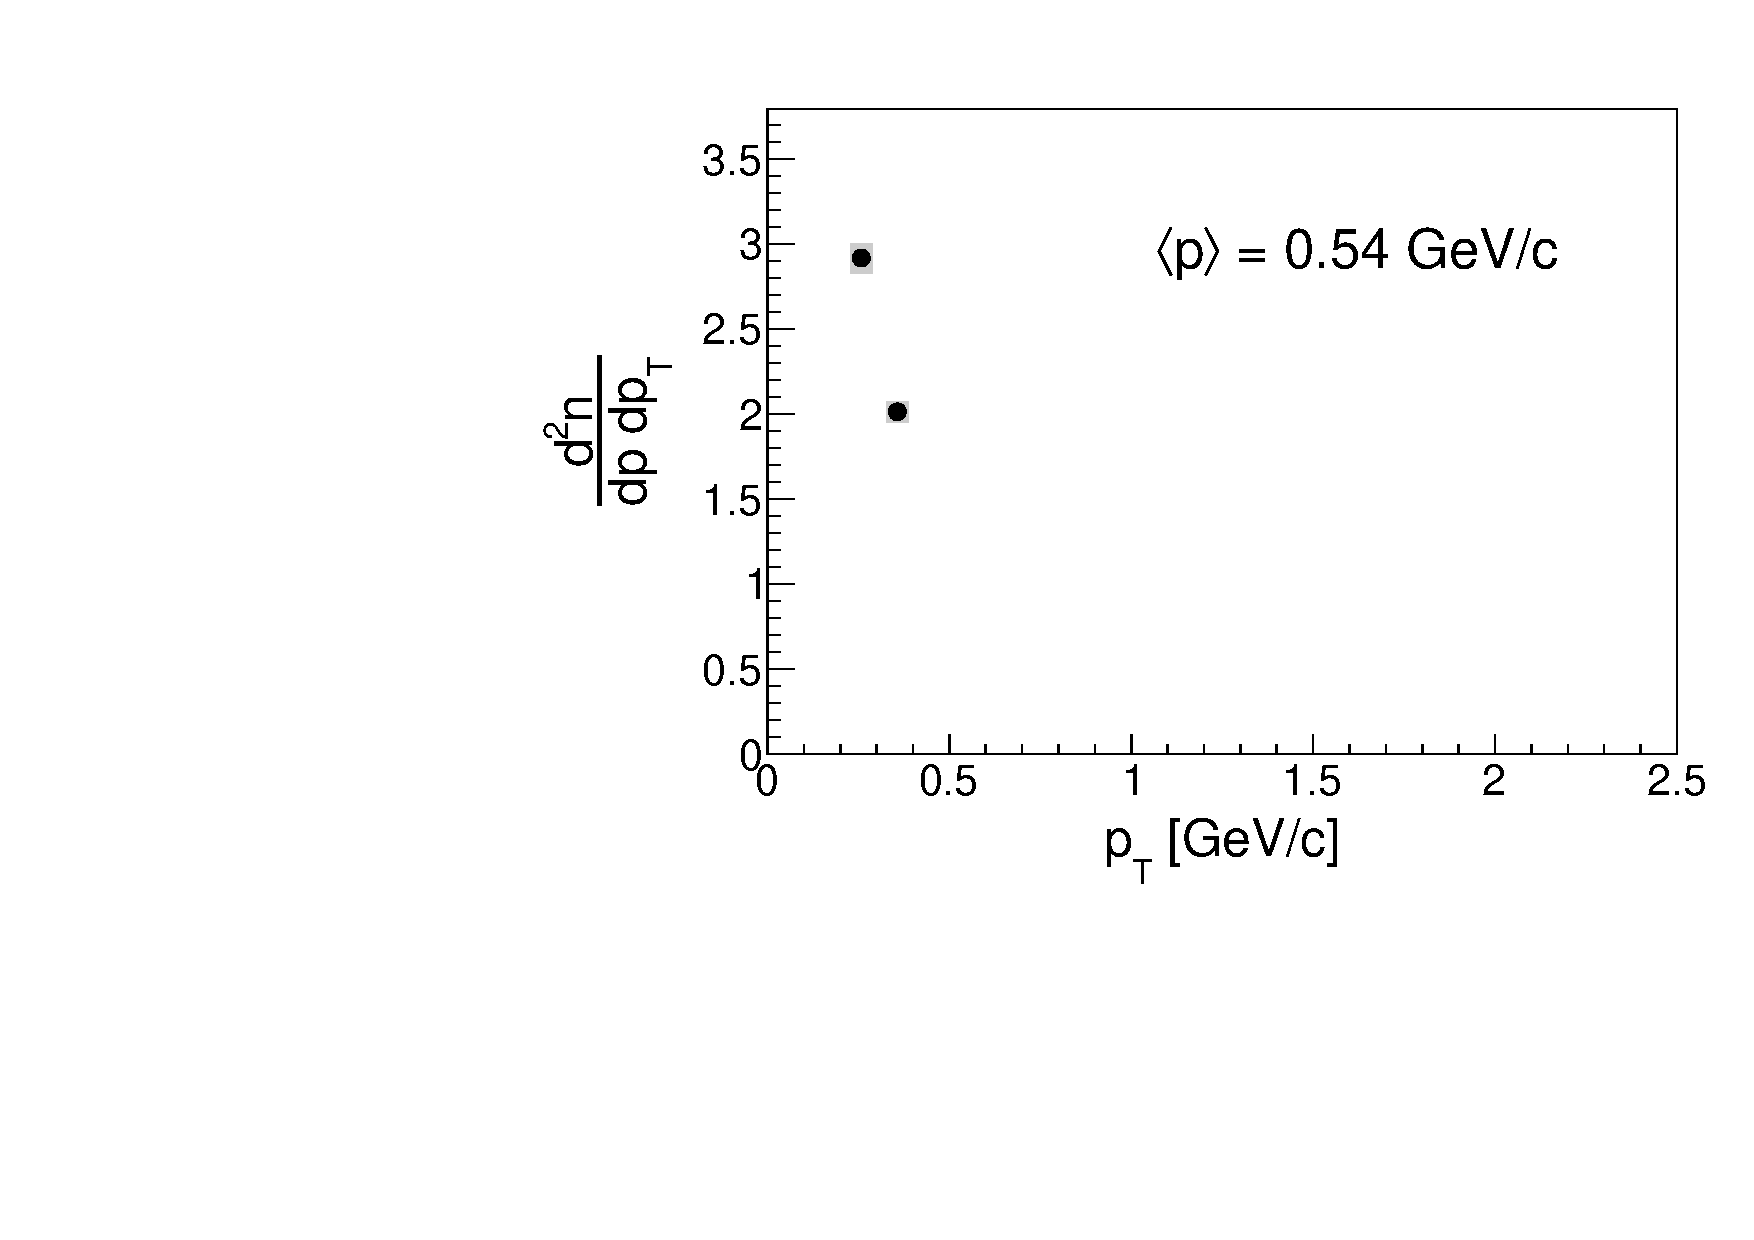
\includegraphics[clip, rviewport=0 0 1 1,width=0.24\textwidth]{spec/spec_pt_158_c1_p1_x7}
  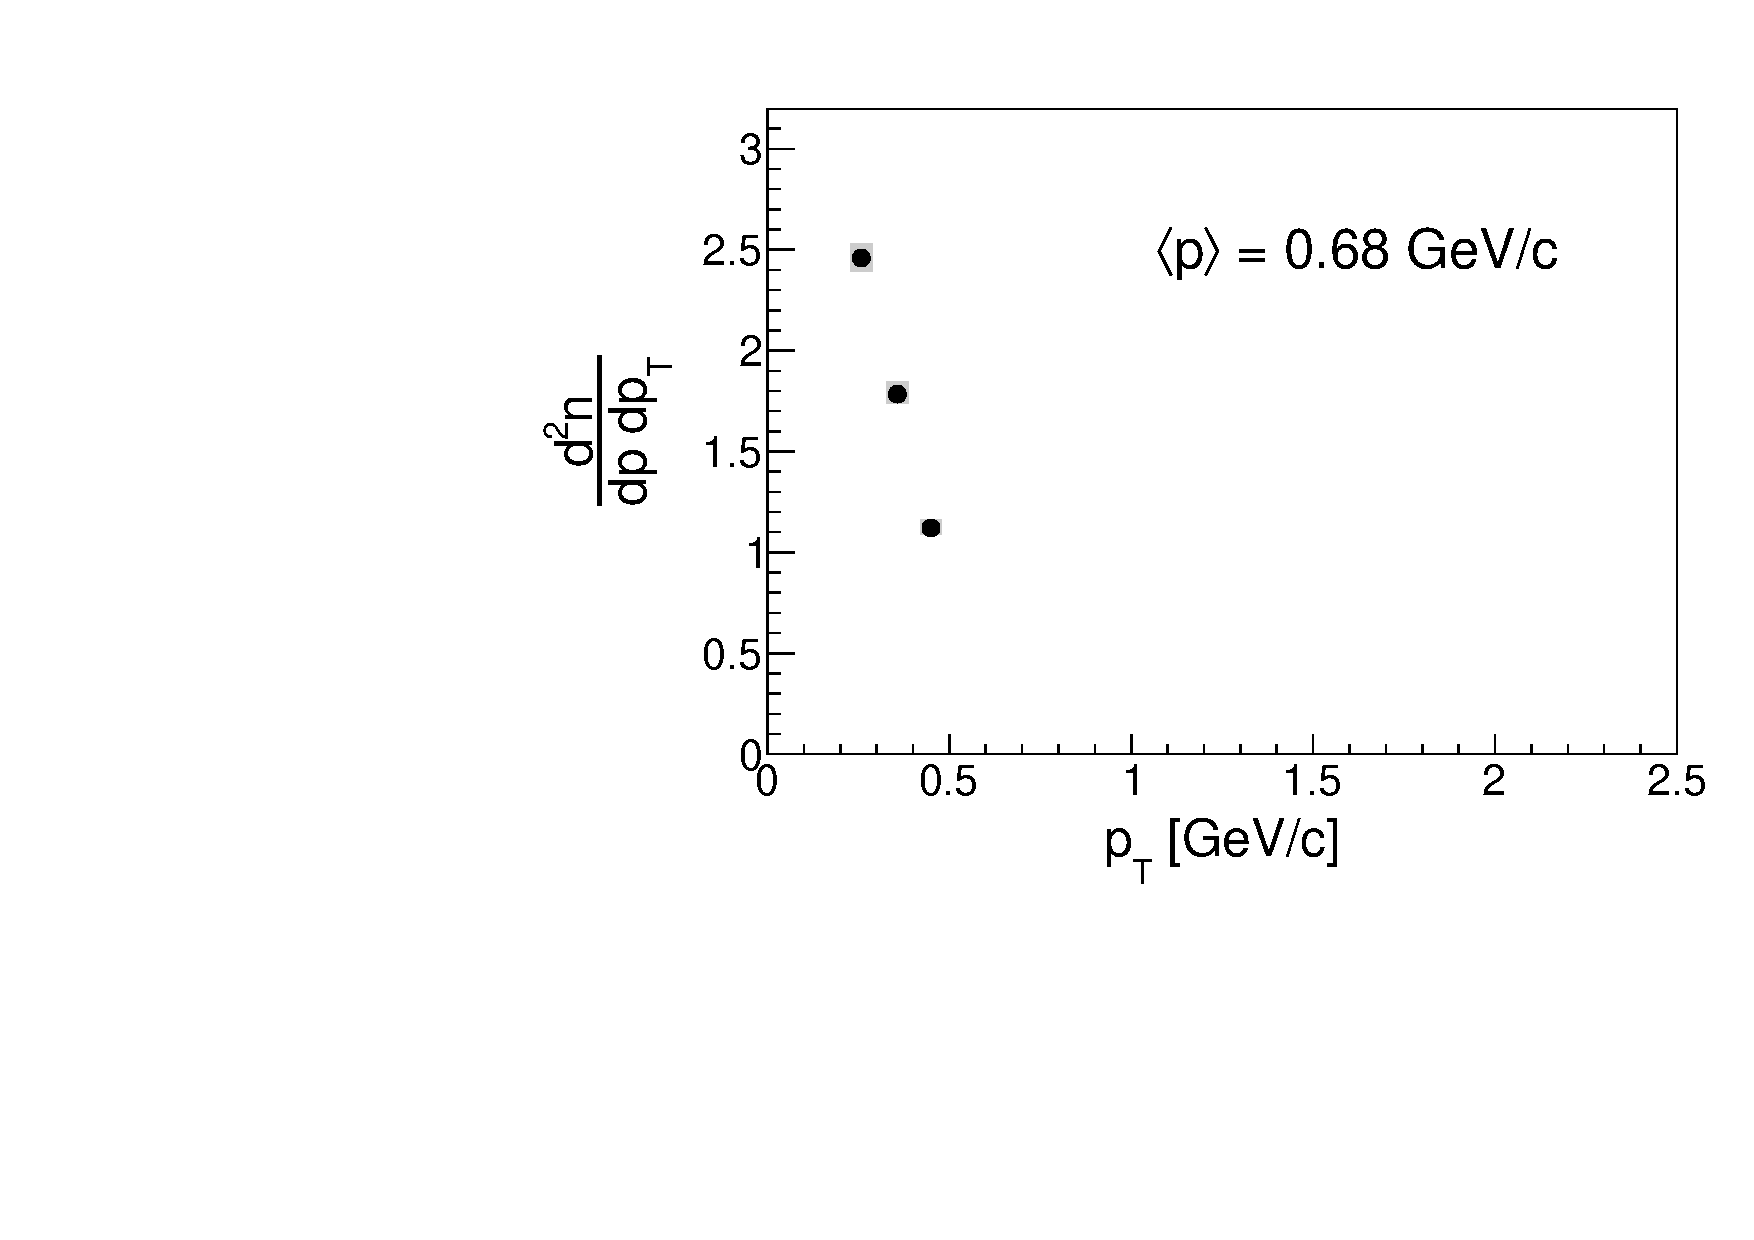
\includegraphics[clip, rviewport=0 0 1 1,width=0.24\textwidth]{spec/spec_pt_158_c1_p1_x8}
  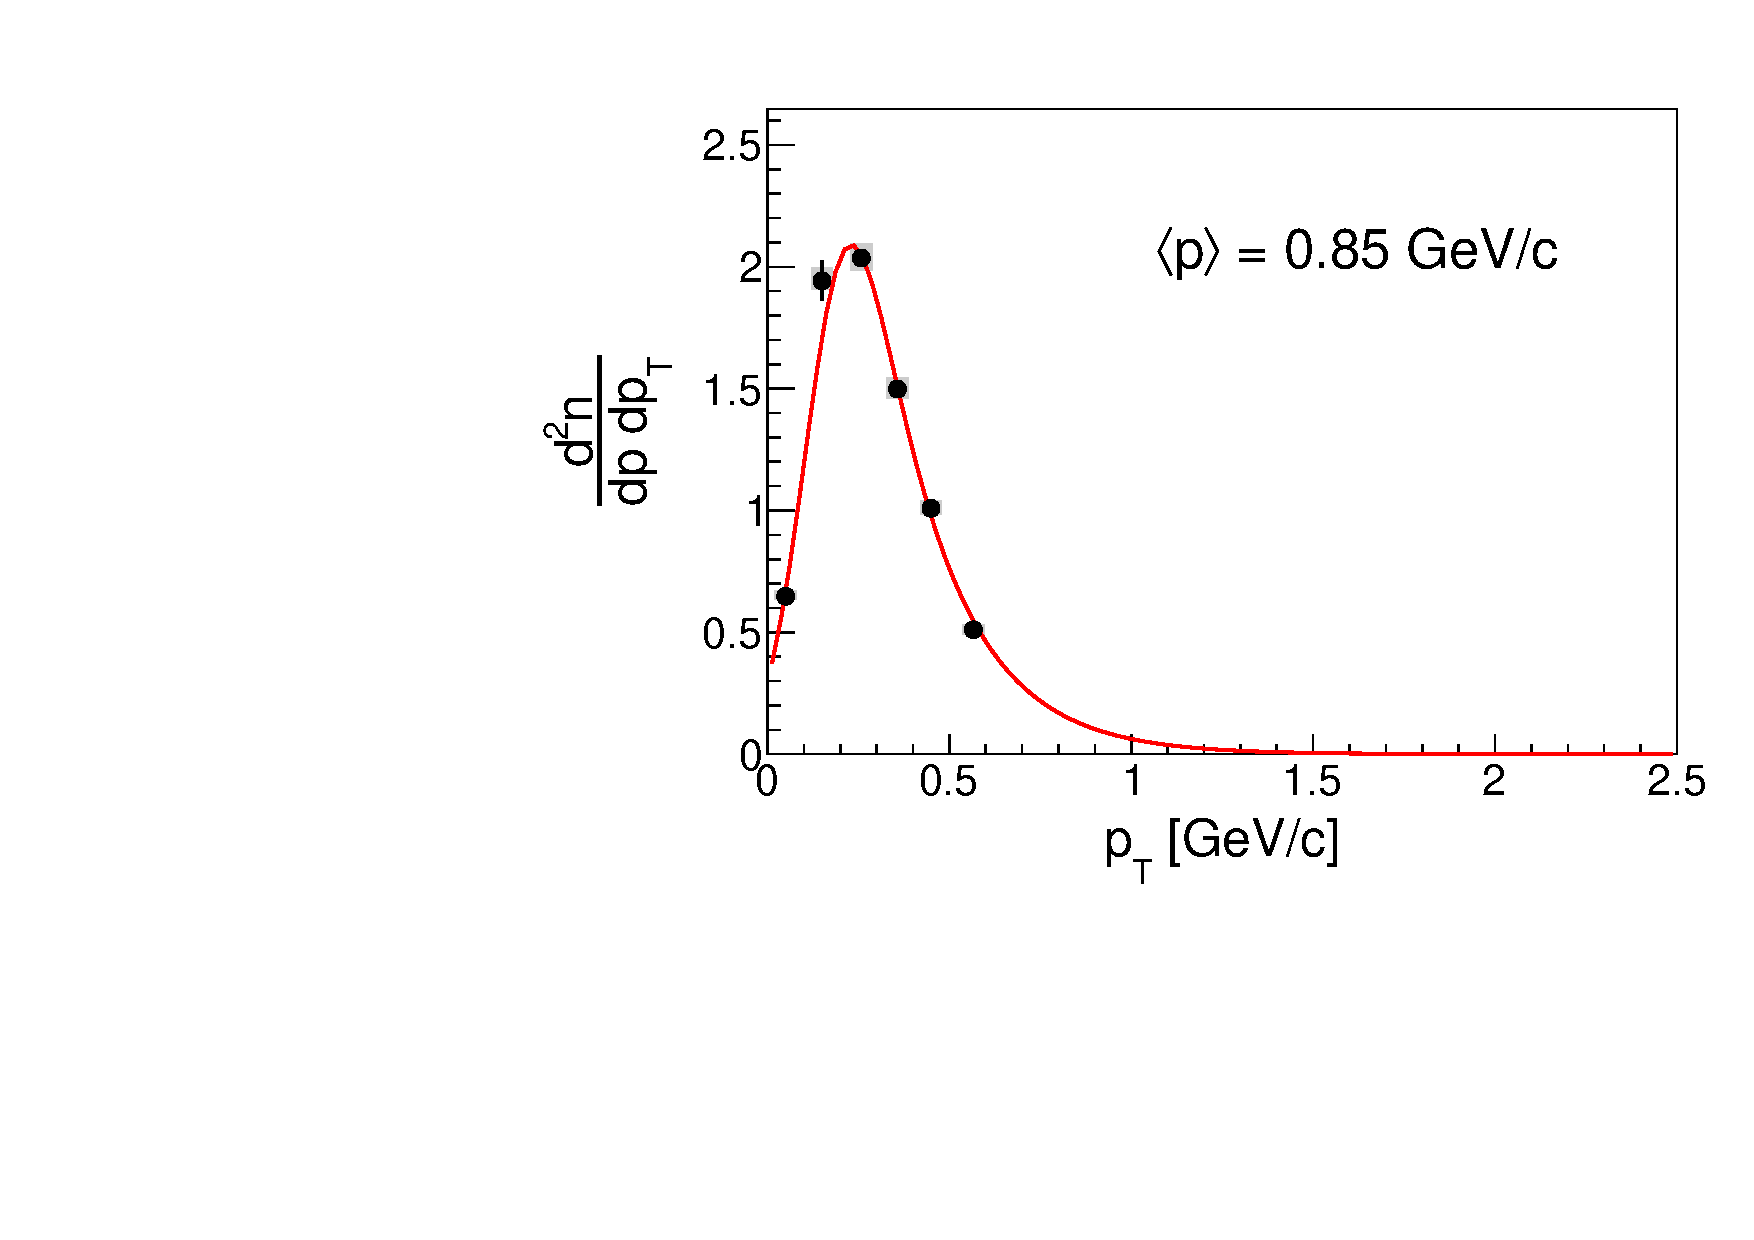
\includegraphics[clip, rviewport=0 0 1 1,width=0.24\textwidth]{spec/spec_pt_158_c1_p1_x9}
  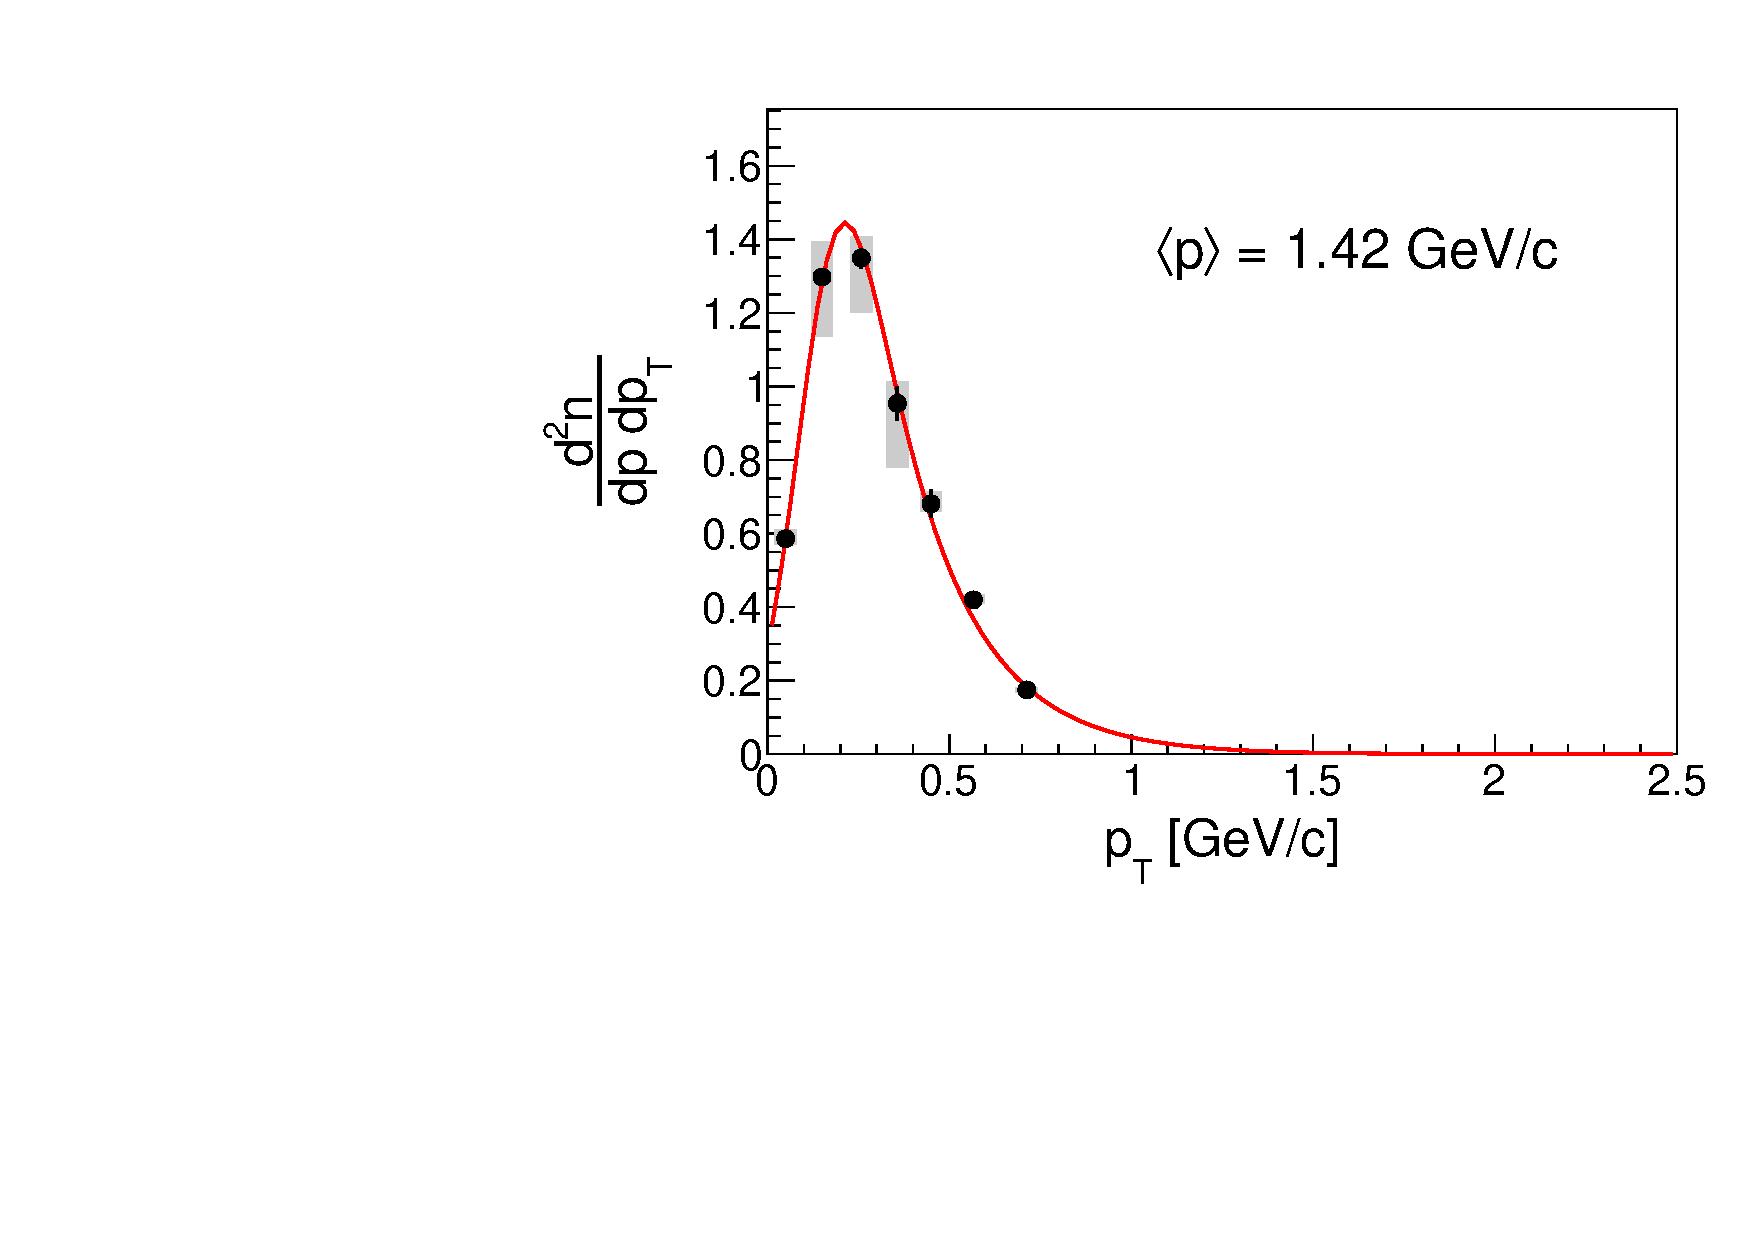
\includegraphics[clip, rviewport=0 0 1 1,width=0.24\textwidth]{spec/spec_pt_158_c1_p1_x11}

  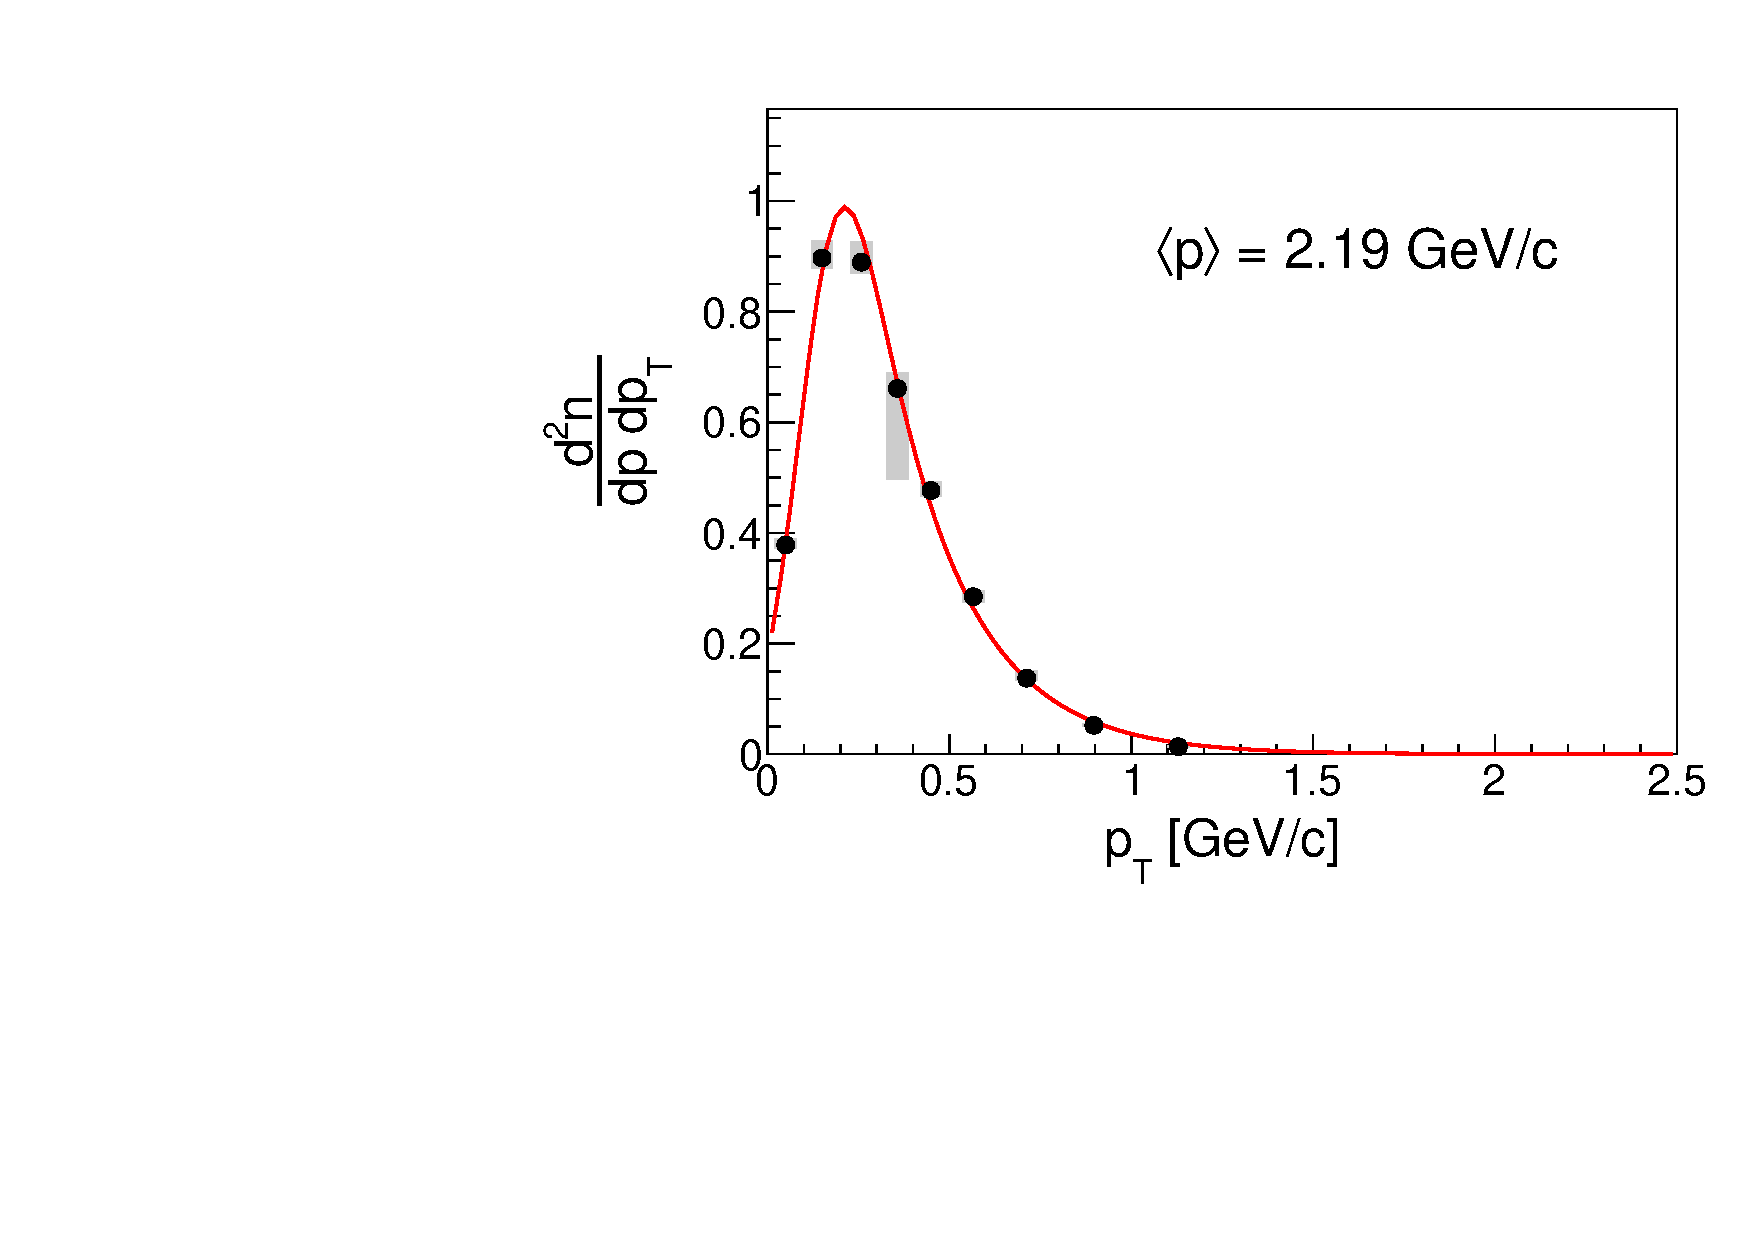
\includegraphics[clip, rviewport=0 0 1 1,width=0.24\textwidth]{spec/spec_pt_158_c1_p1_x13}
  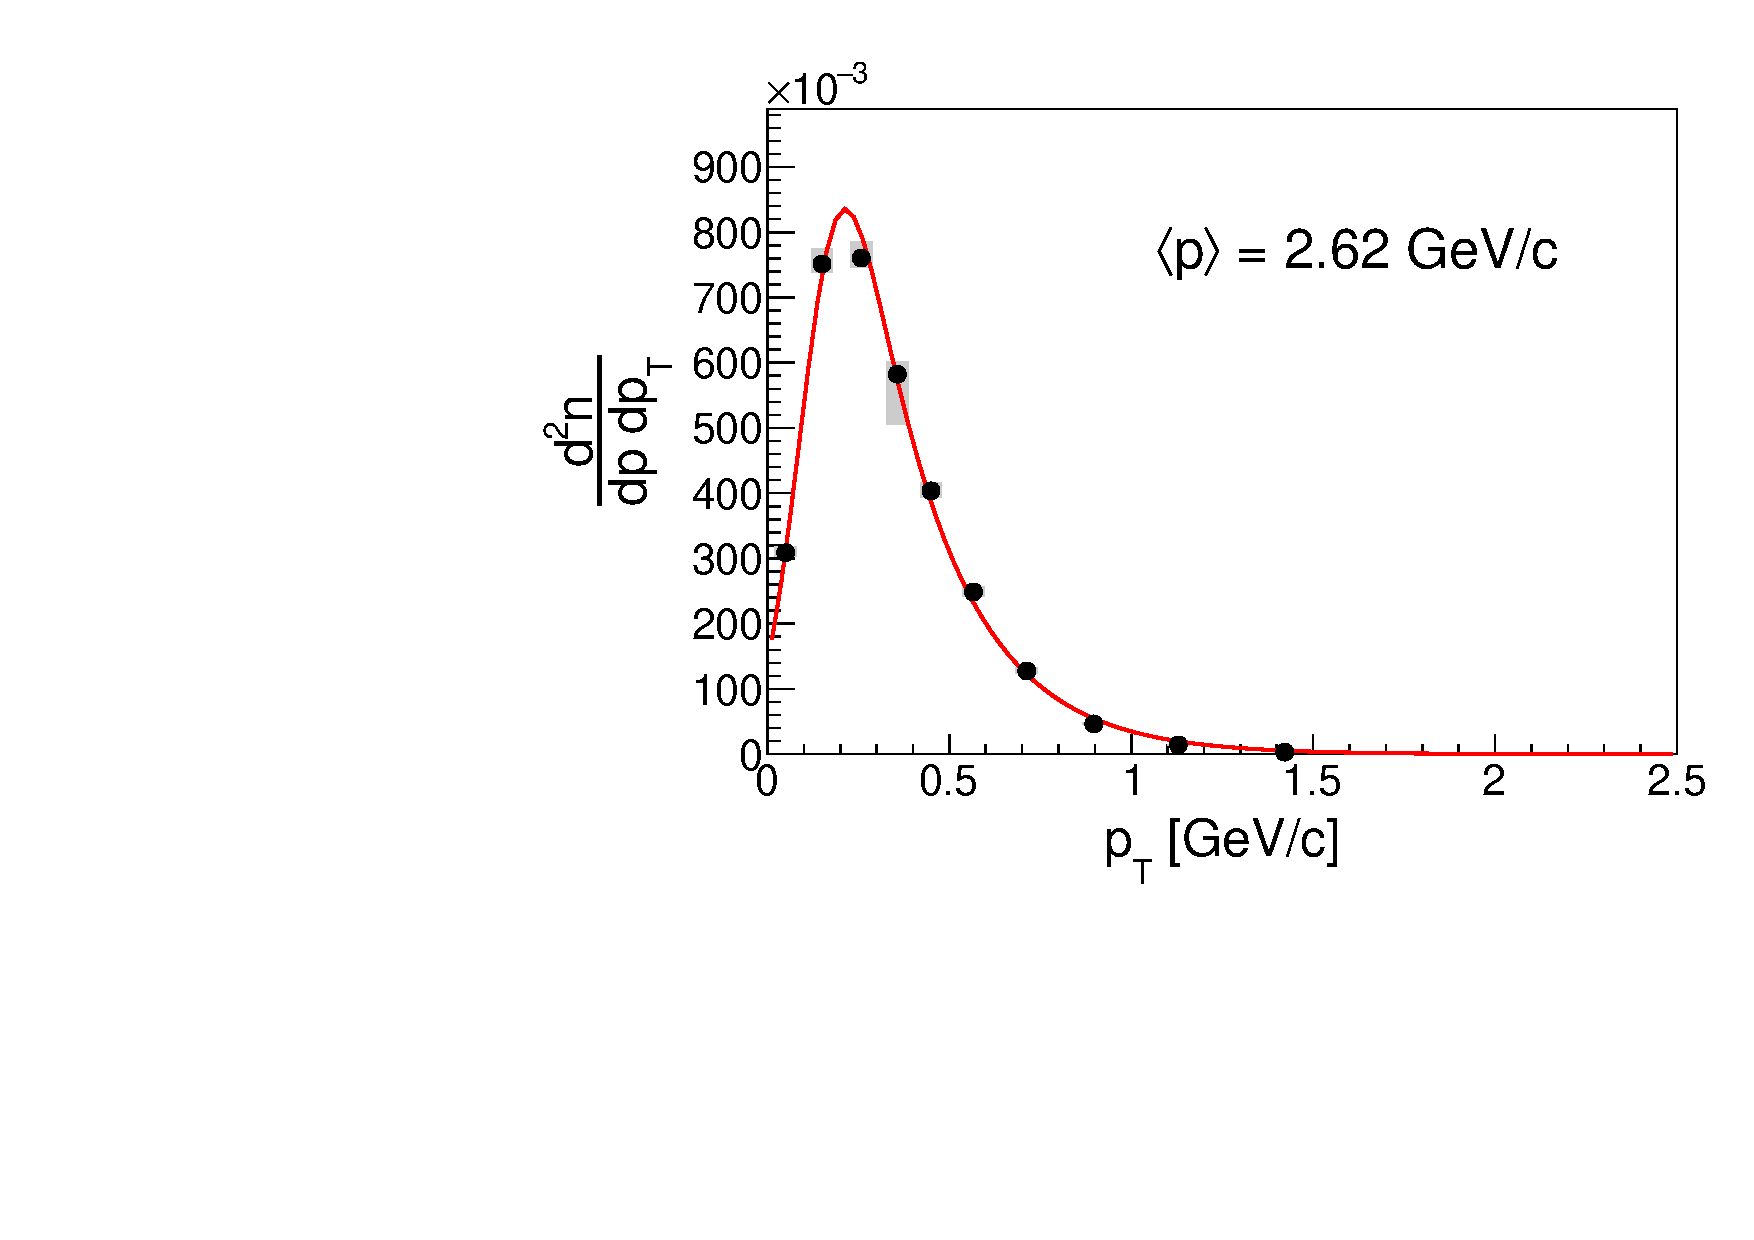
\includegraphics[clip, rviewport=0 0 1 1,width=0.24\textwidth]{spec/spec_pt_158_c1_p1_x14}
  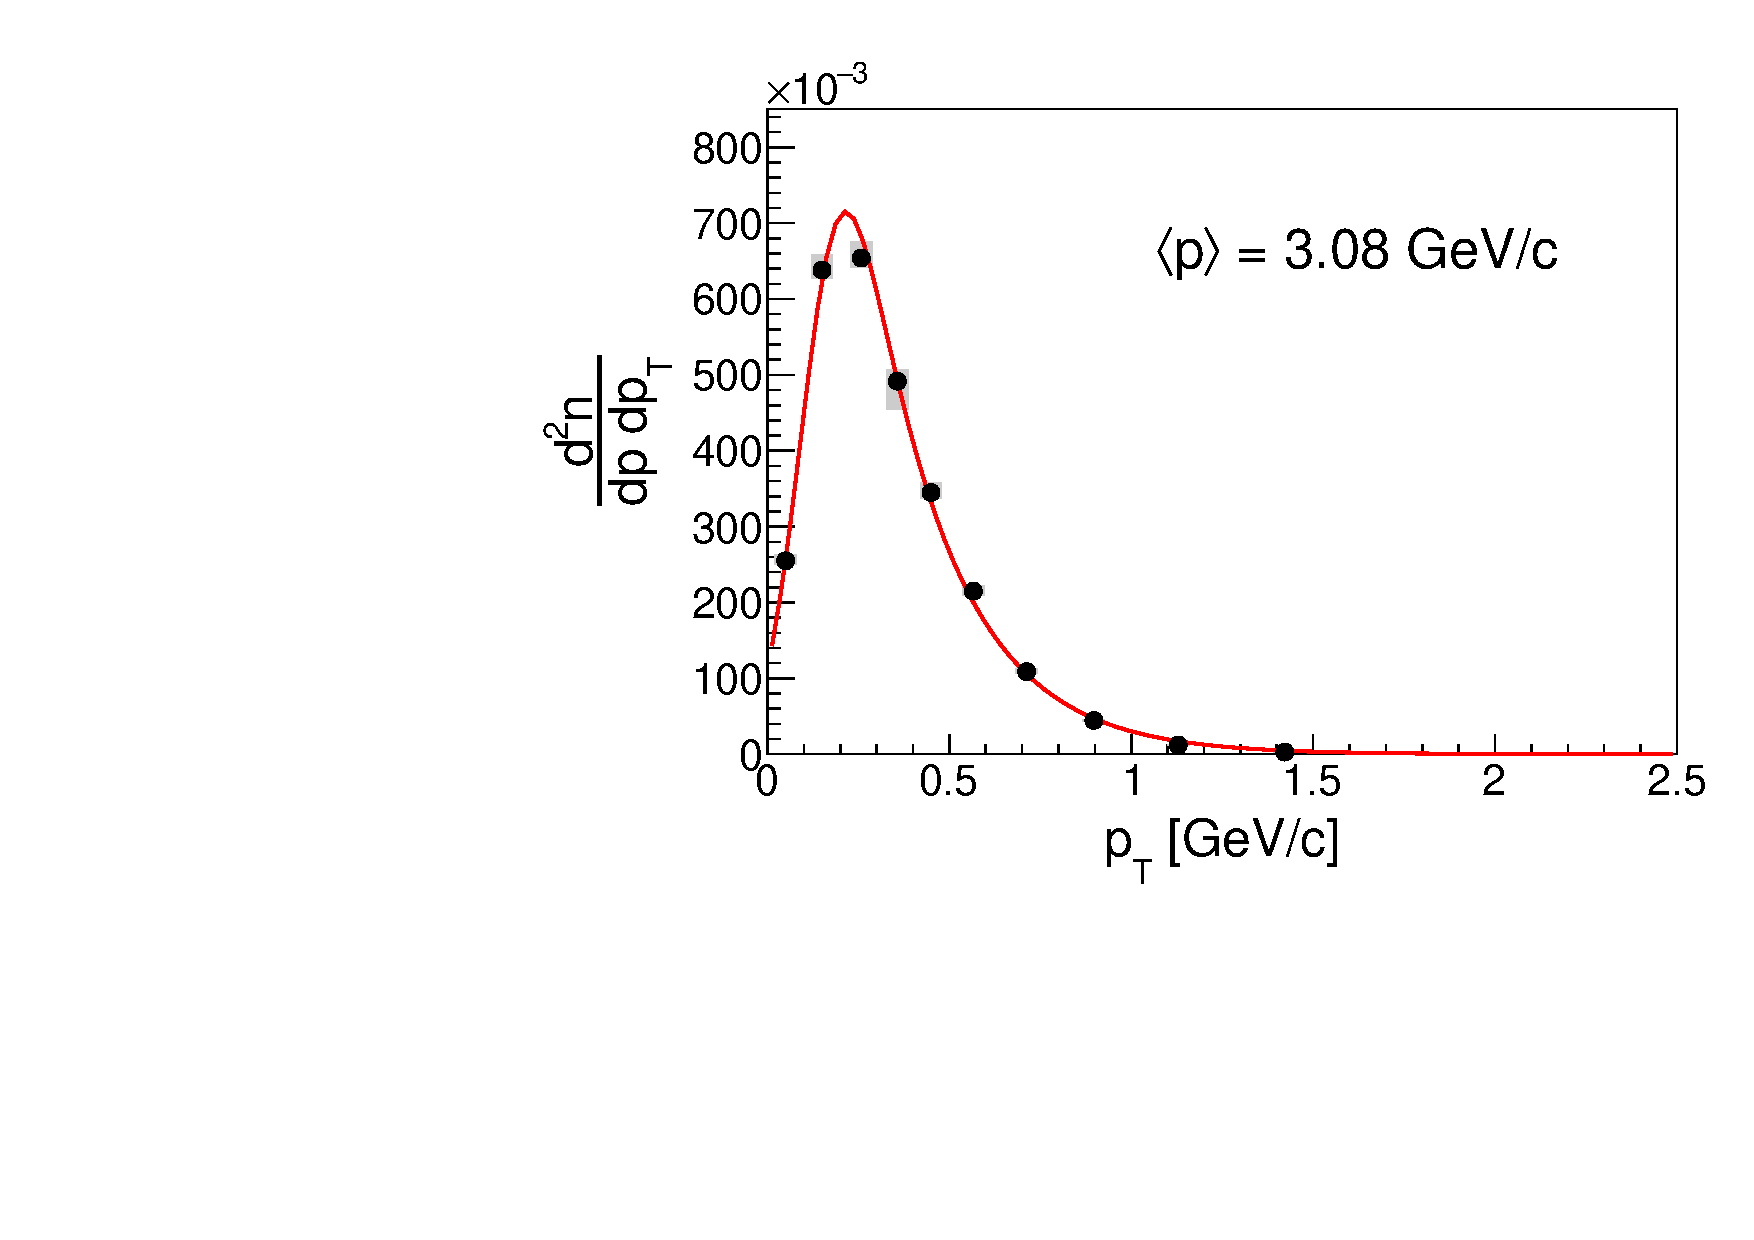
\includegraphics[clip, rviewport=0 0 1 1,width=0.24\textwidth]{spec/spec_pt_158_c1_p1_x15}
  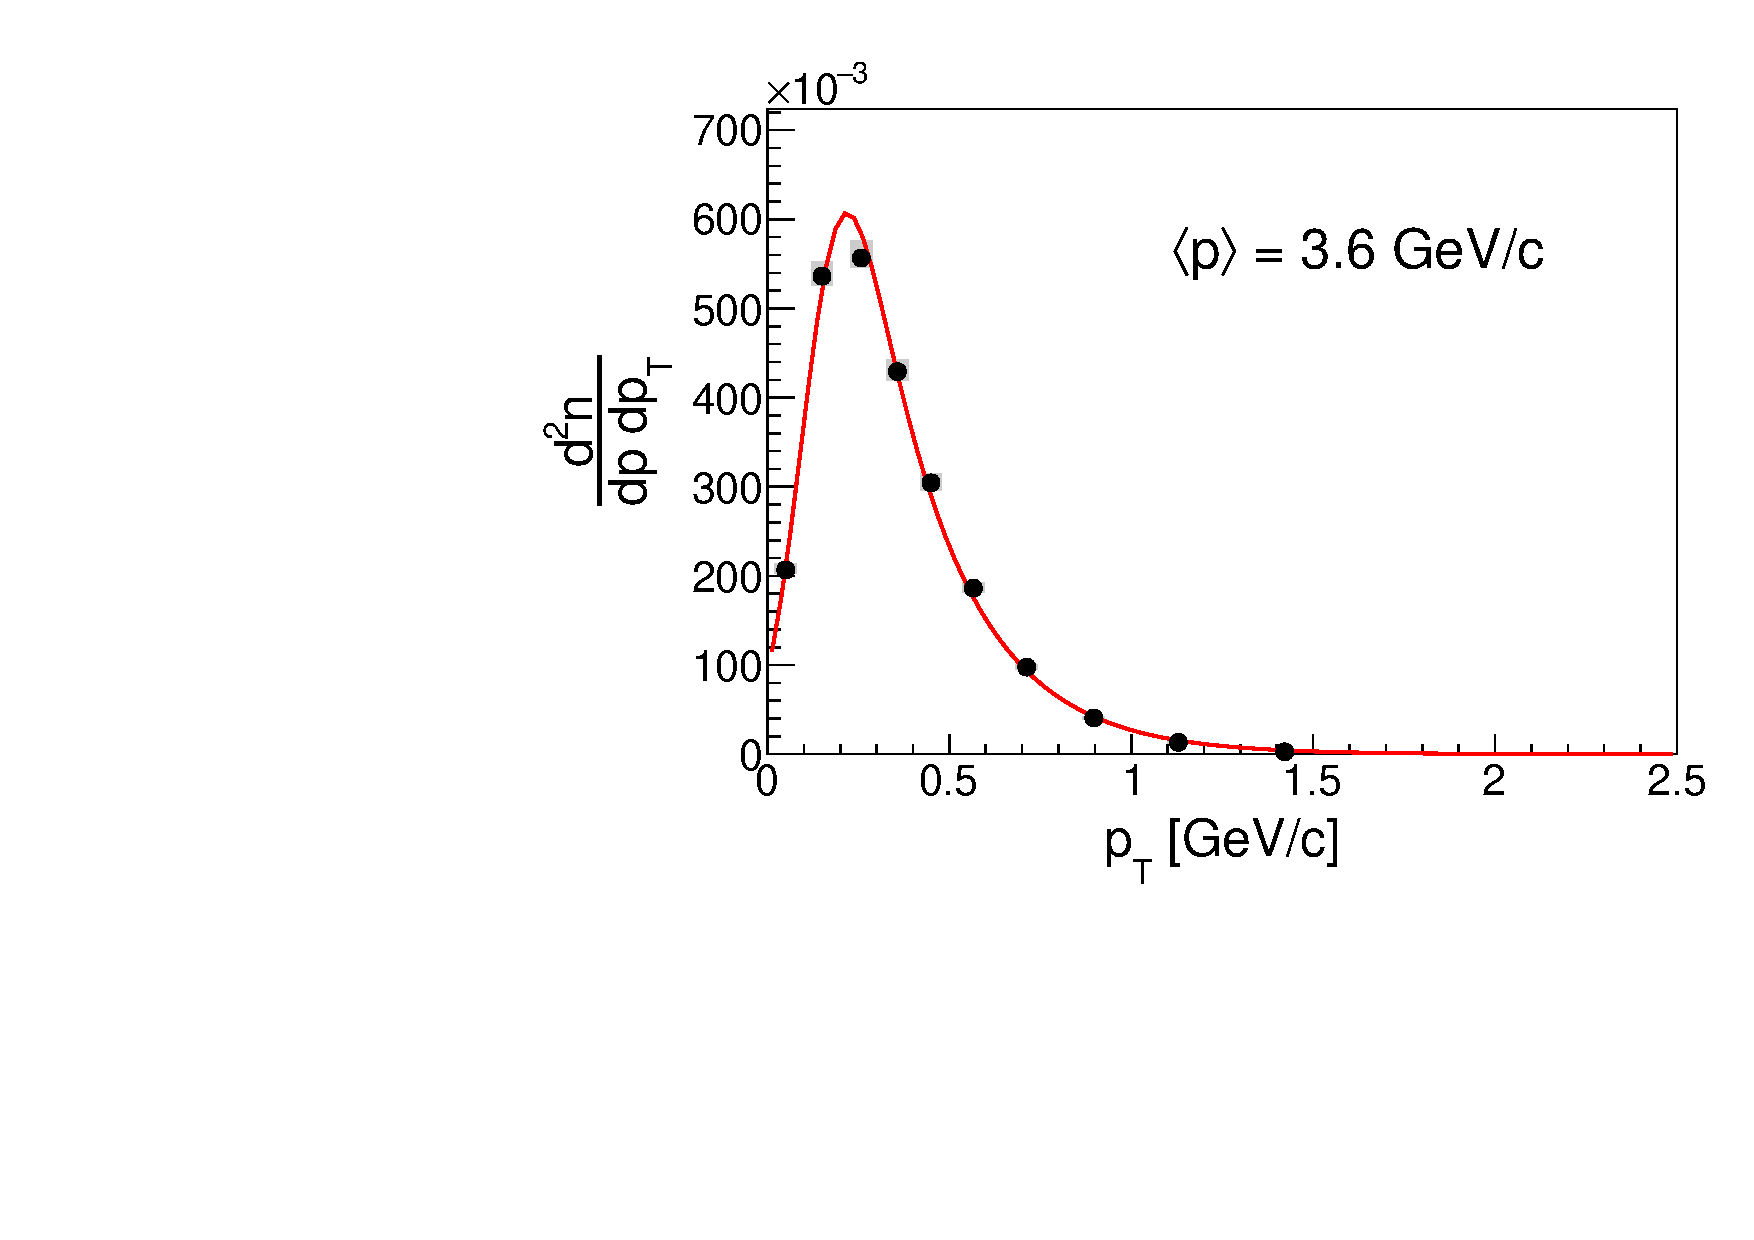
\includegraphics[clip, rviewport=0 0 1 1,width=0.24\textwidth]{spec/spec_pt_158_c1_p1_x16}

  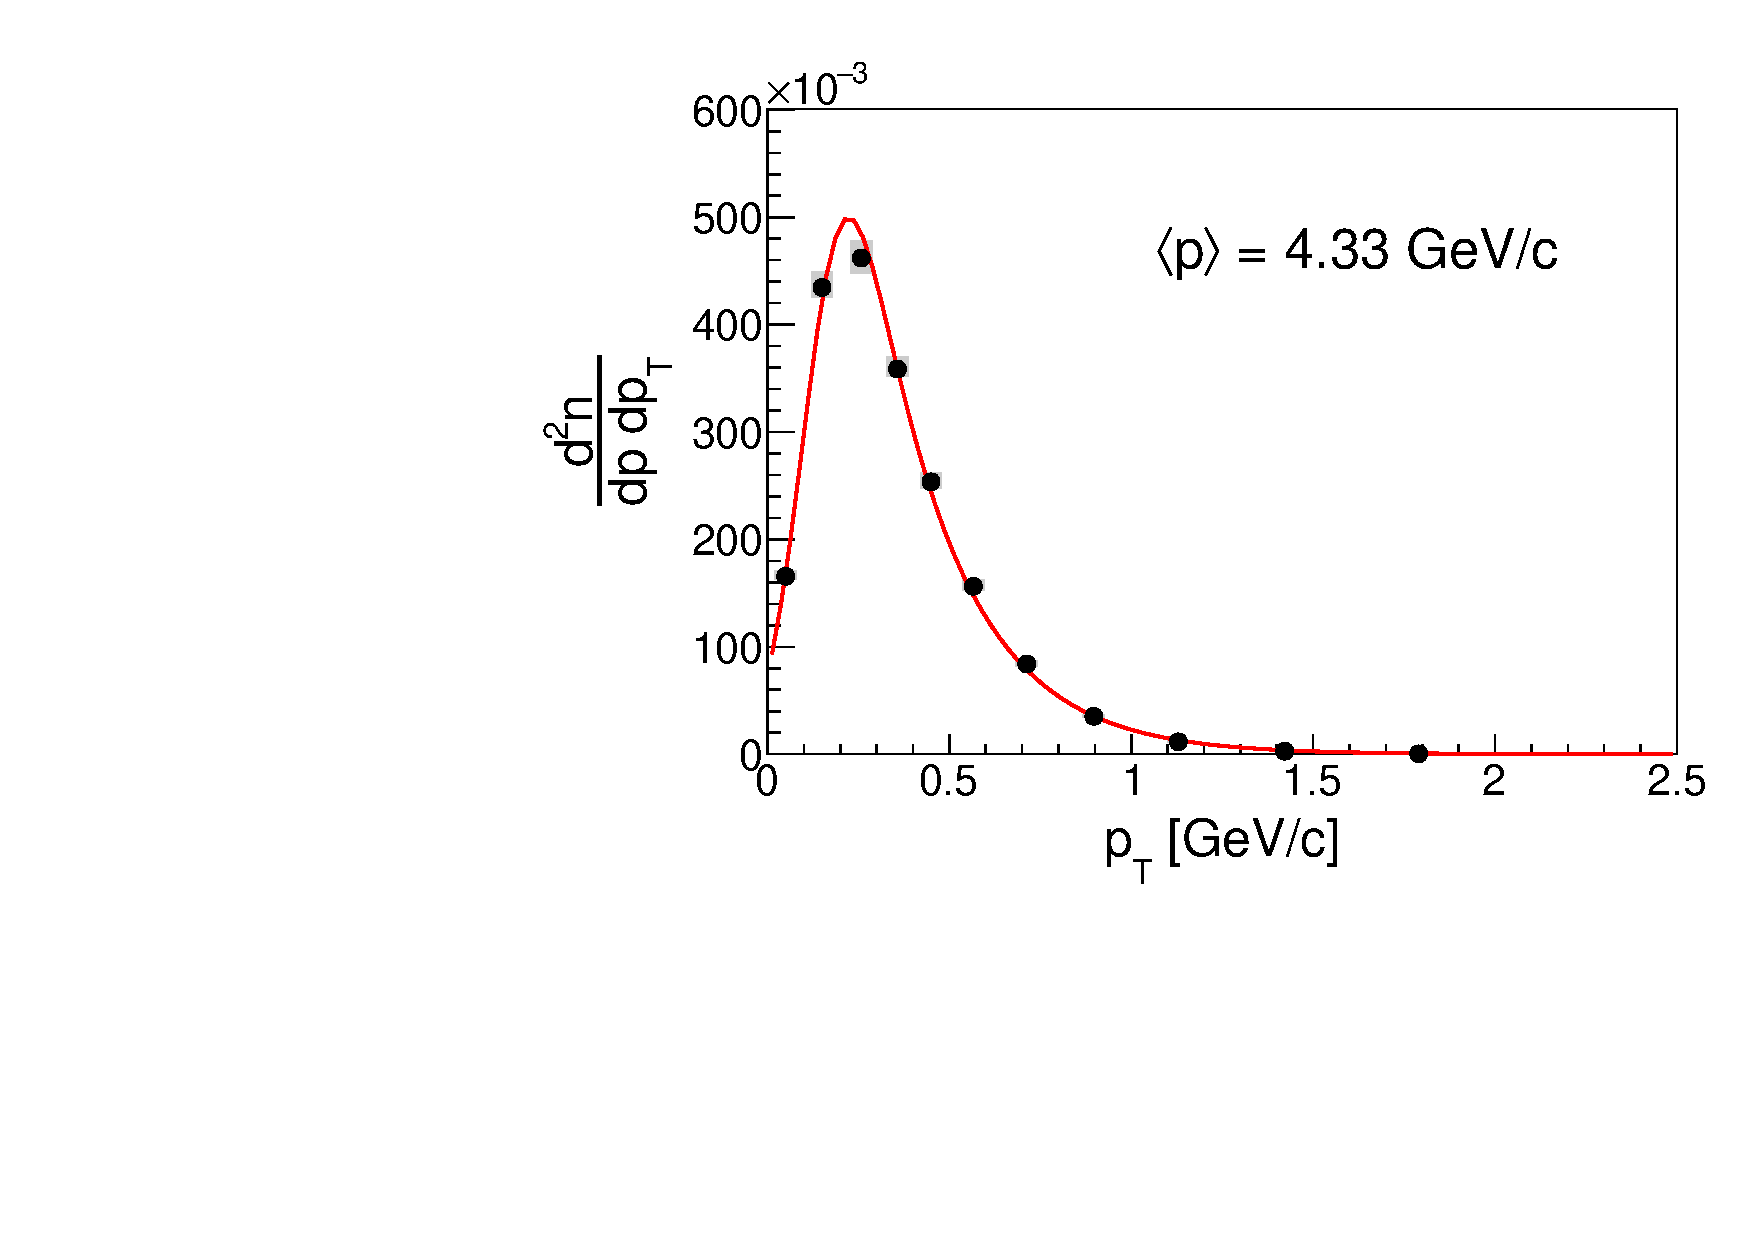
\includegraphics[clip, rviewport=0 0 1 1,width=0.24\textwidth]{spec/spec_pt_158_c1_p1_x17}
  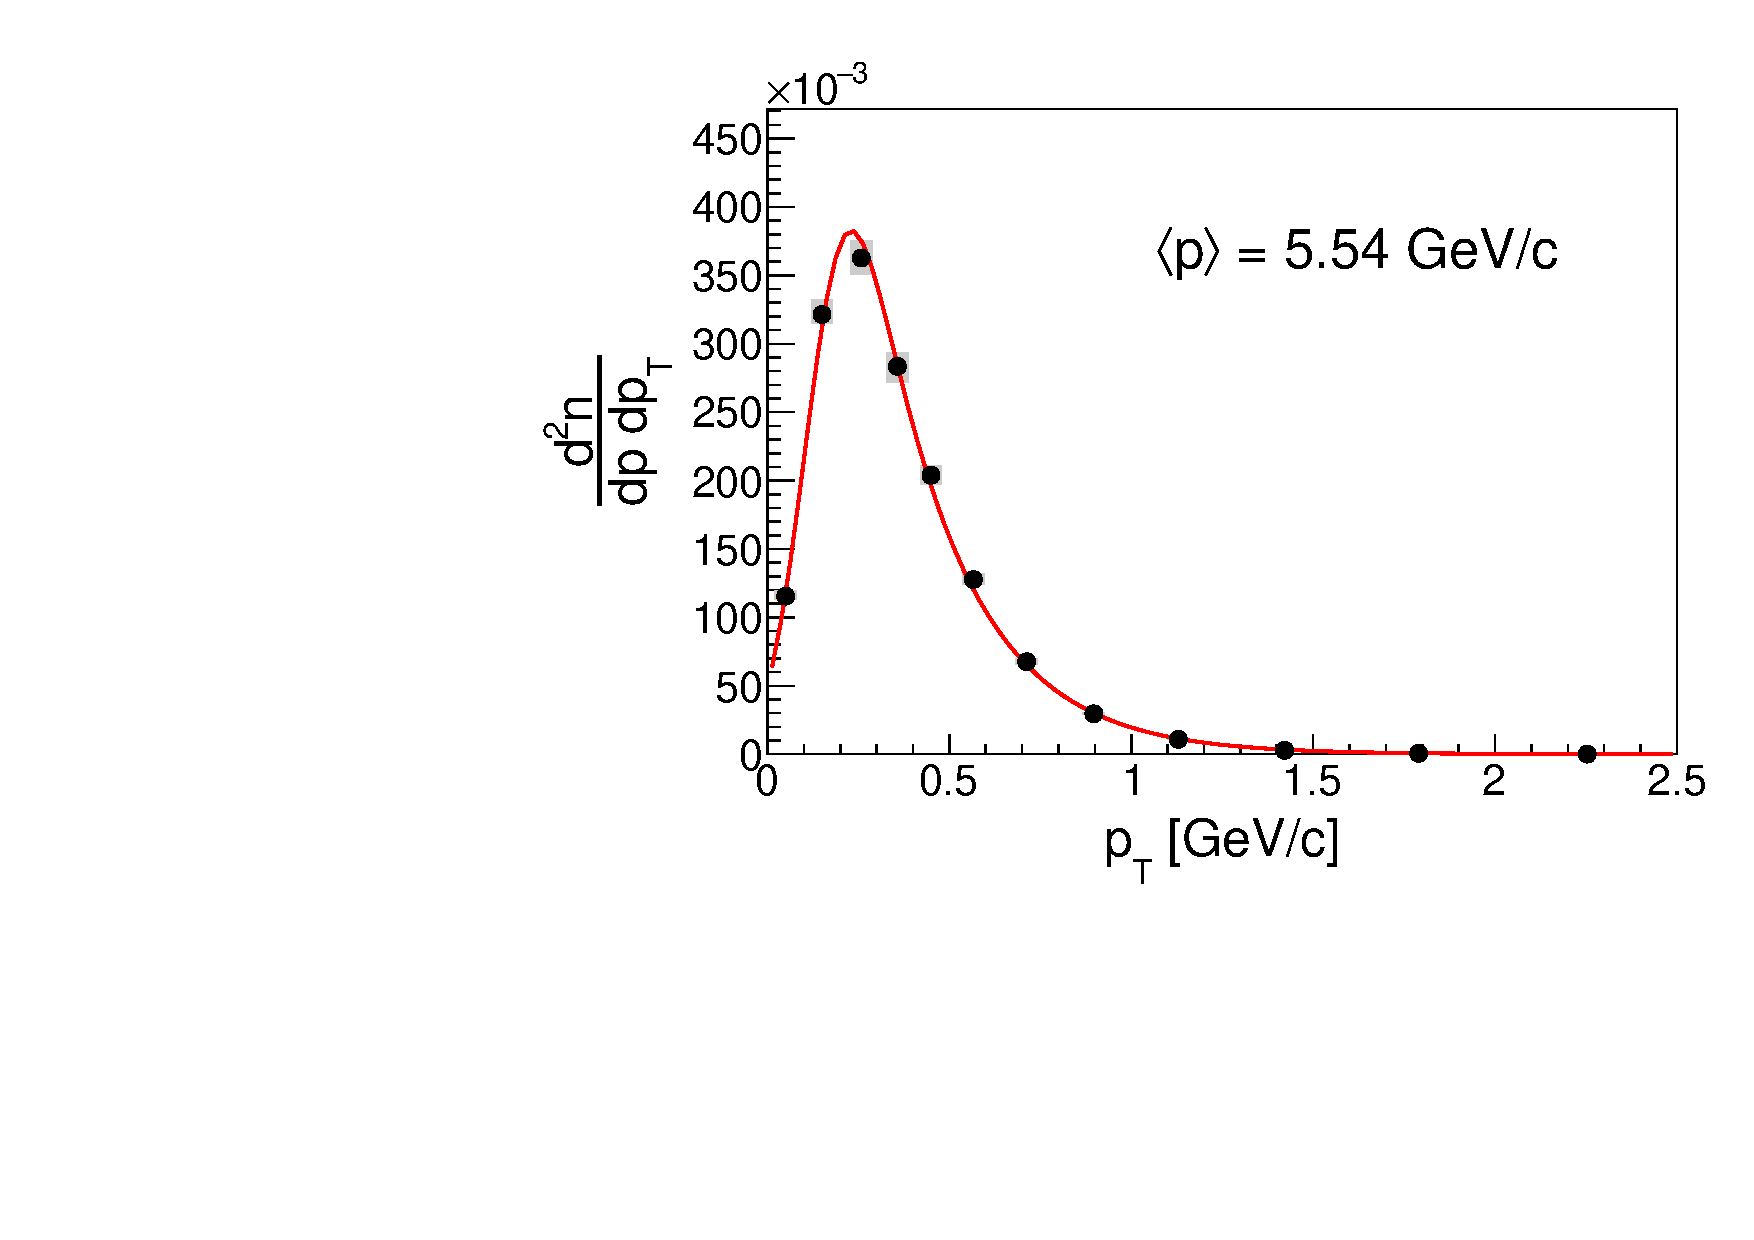
\includegraphics[clip, rviewport=0 0 1 1,width=0.24\textwidth]{spec/spec_pt_158_c1_p1_x18}
  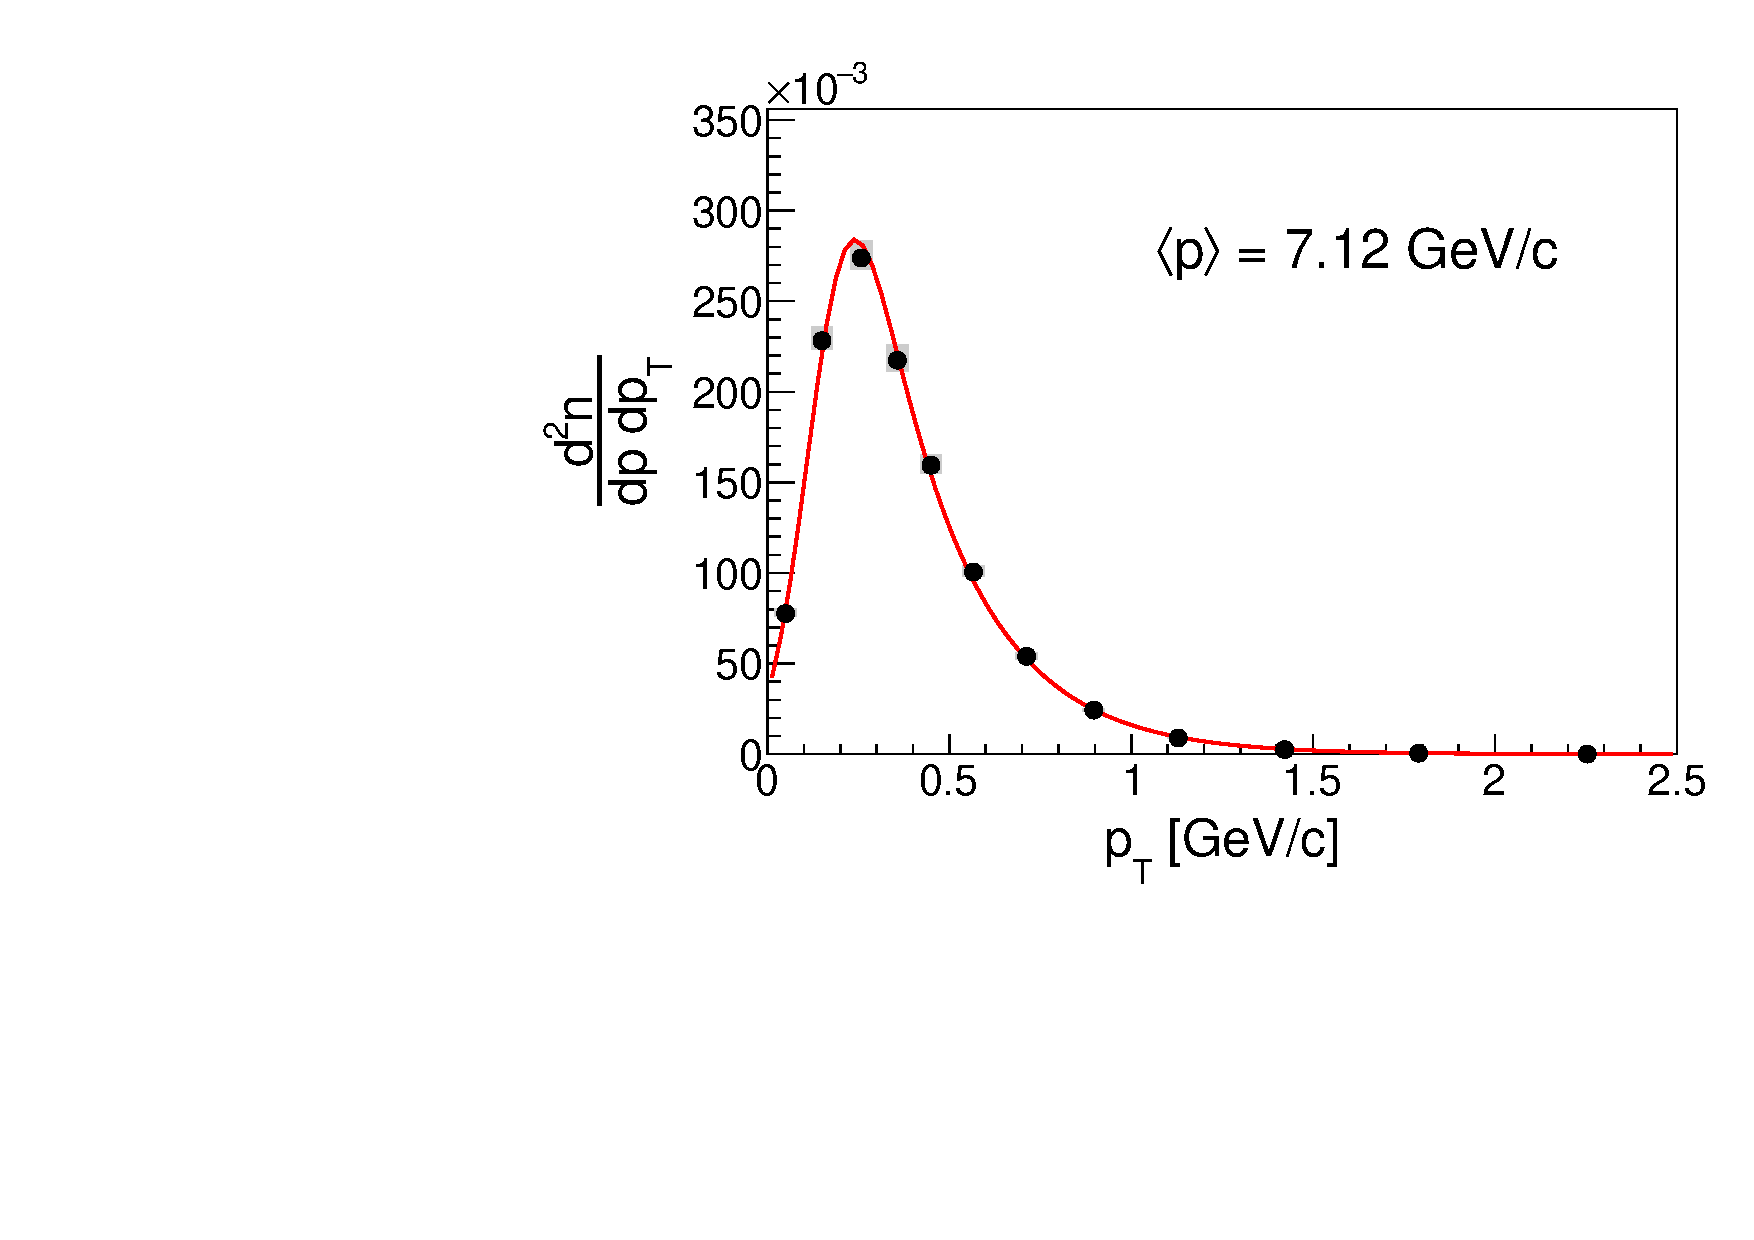
\includegraphics[clip, rviewport=0 0 1 1,width=0.24\textwidth]{spec/spec_pt_158_c1_p1_x19}
  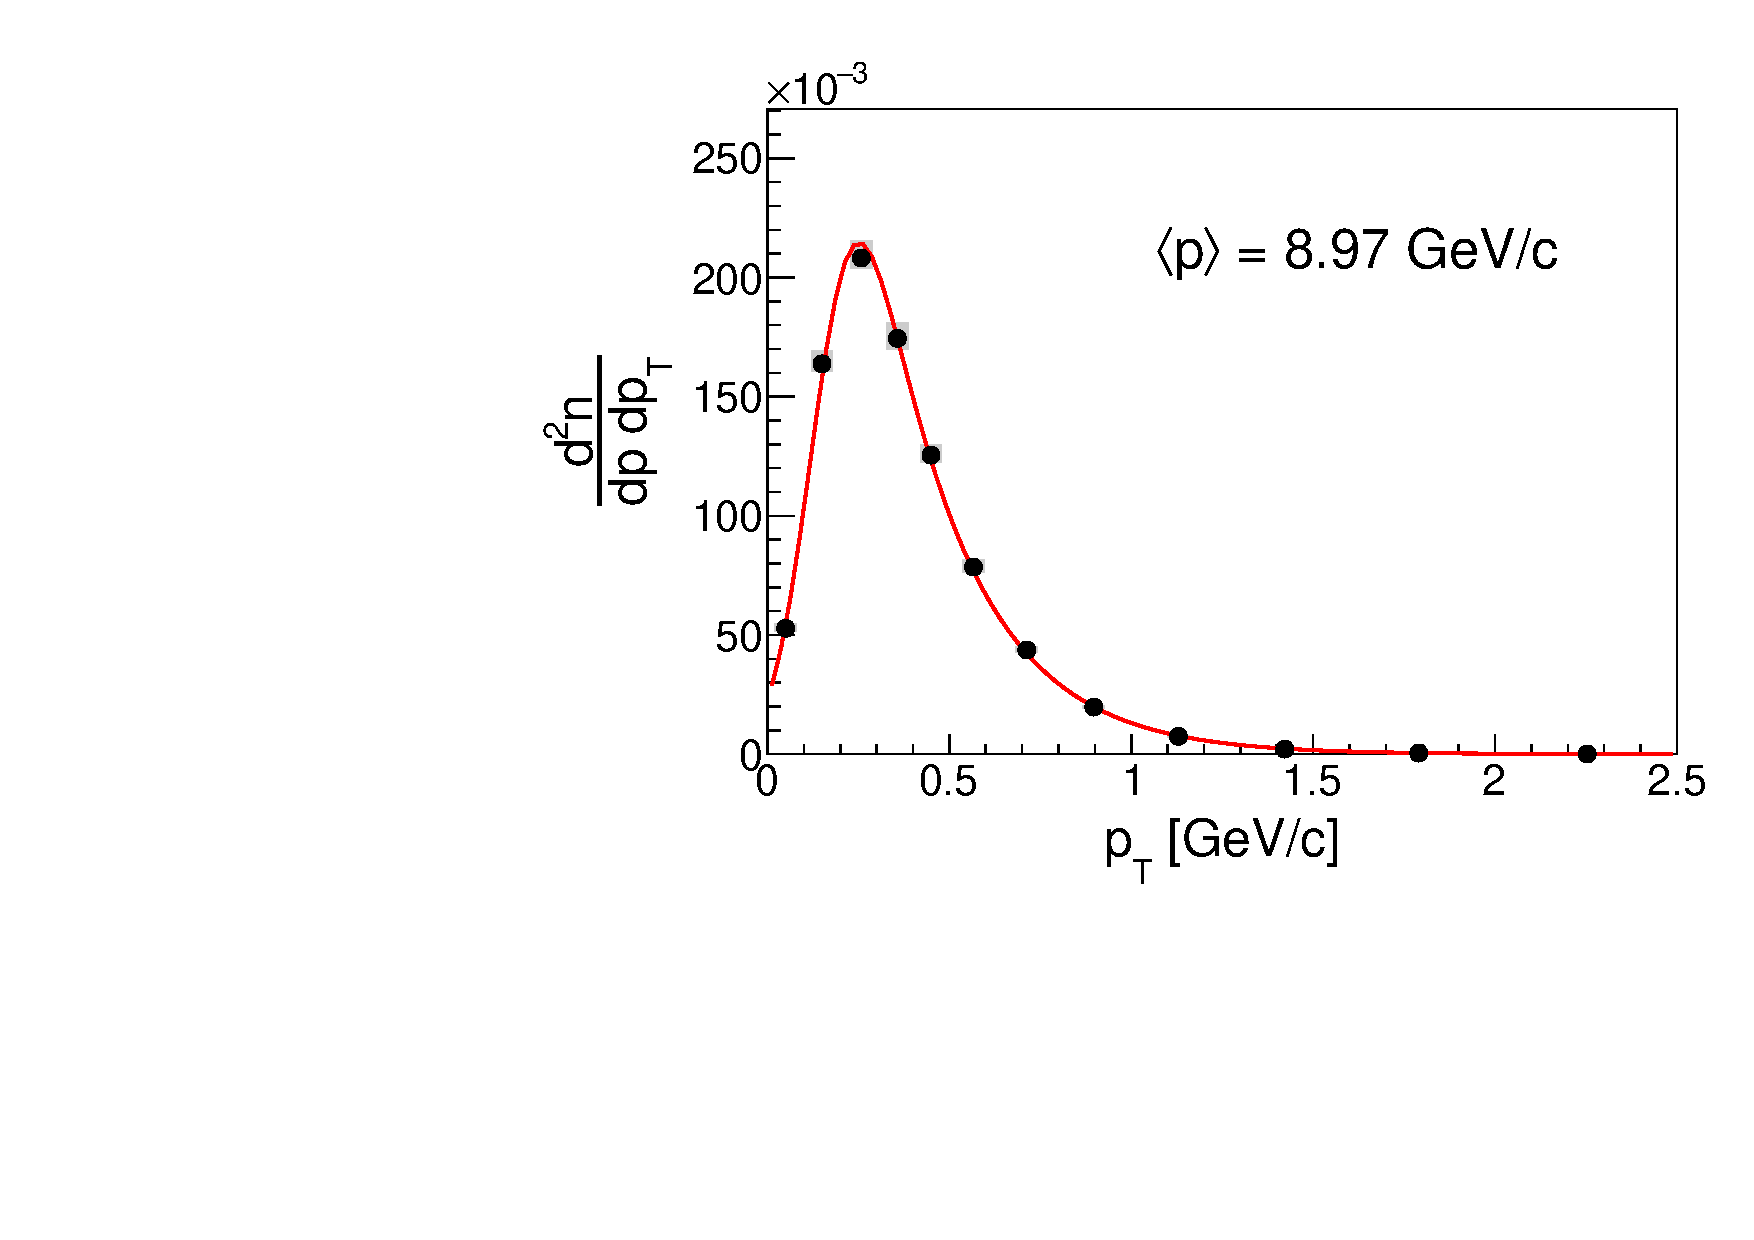
\includegraphics[clip, rviewport=0 0 1 1,width=0.24\textwidth]{spec/spec_pt_158_c1_p1_x20}

  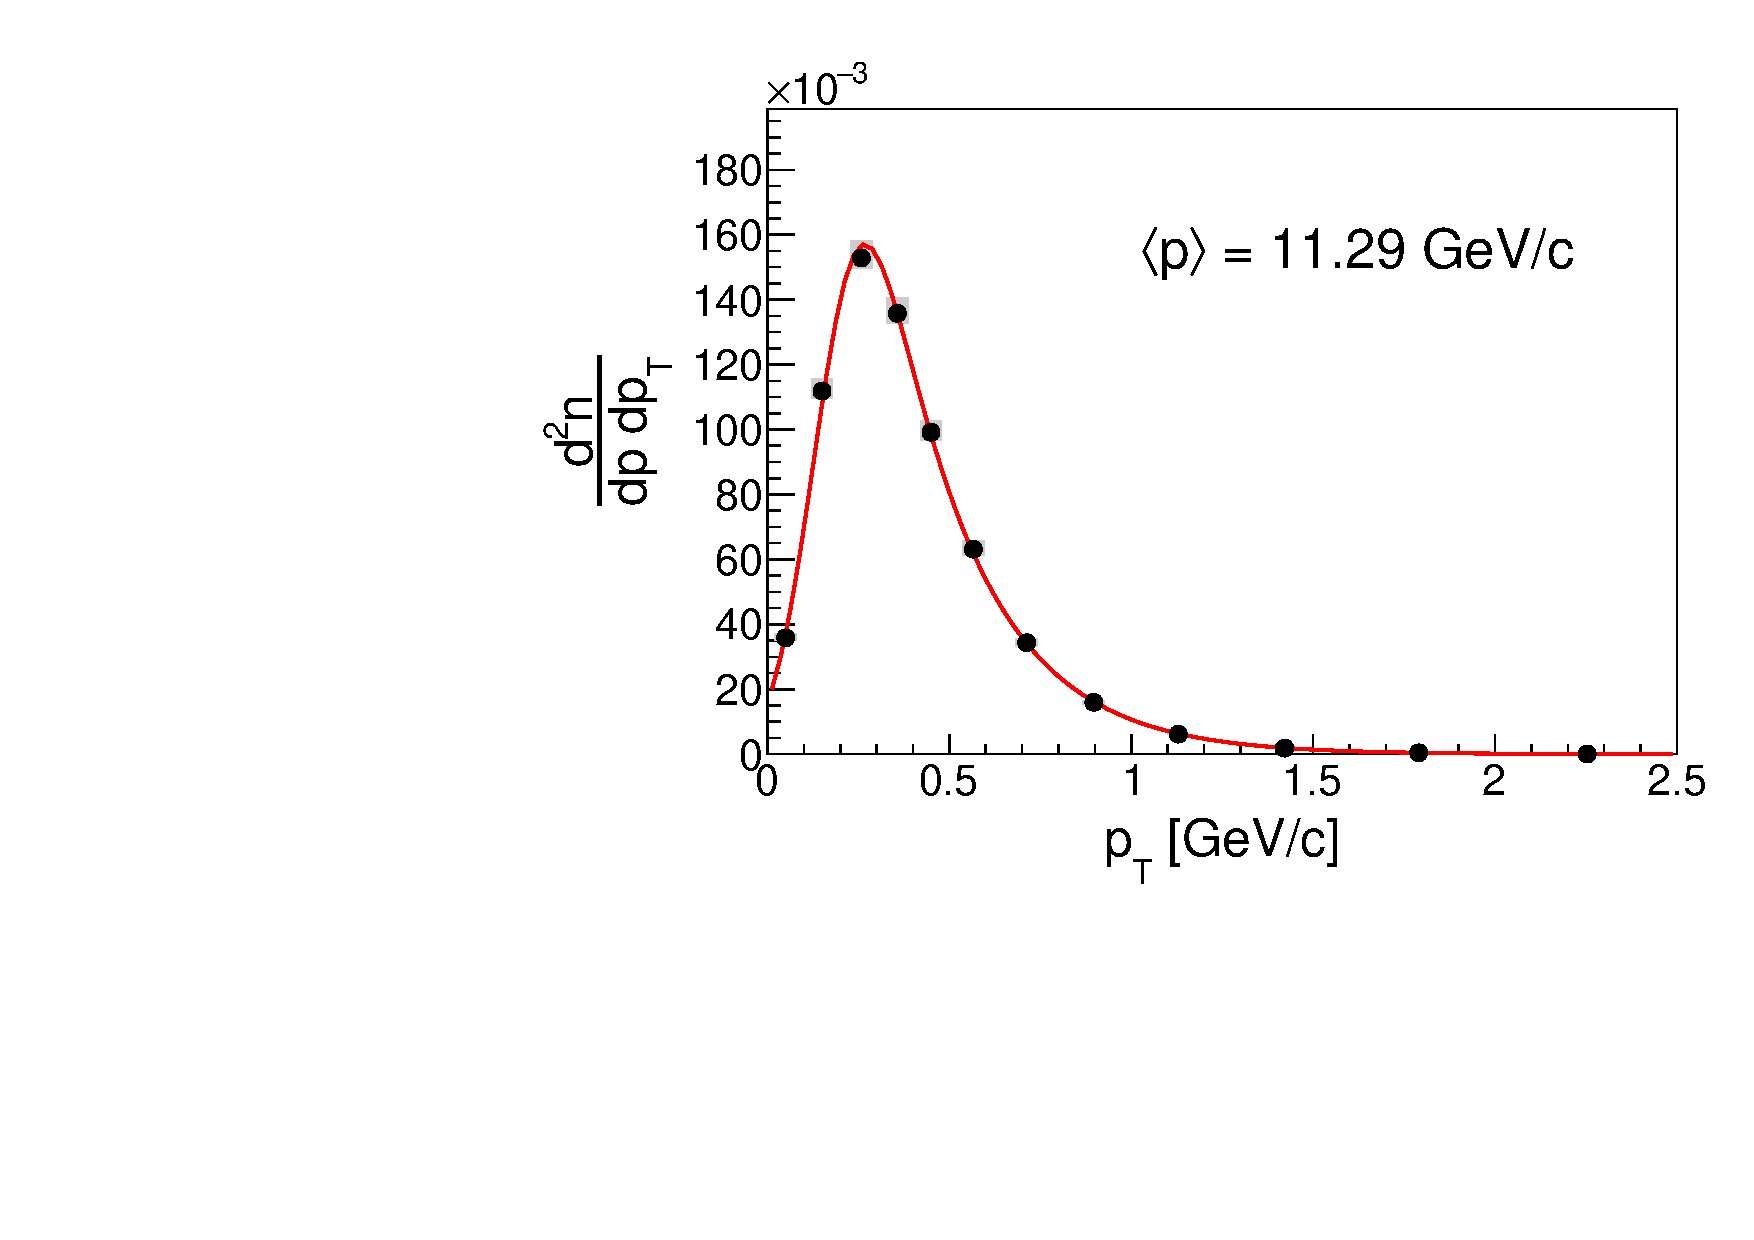
\includegraphics[clip, rviewport=0 0 1 1,width=0.24\textwidth]{spec/spec_pt_158_c1_p1_x21}
  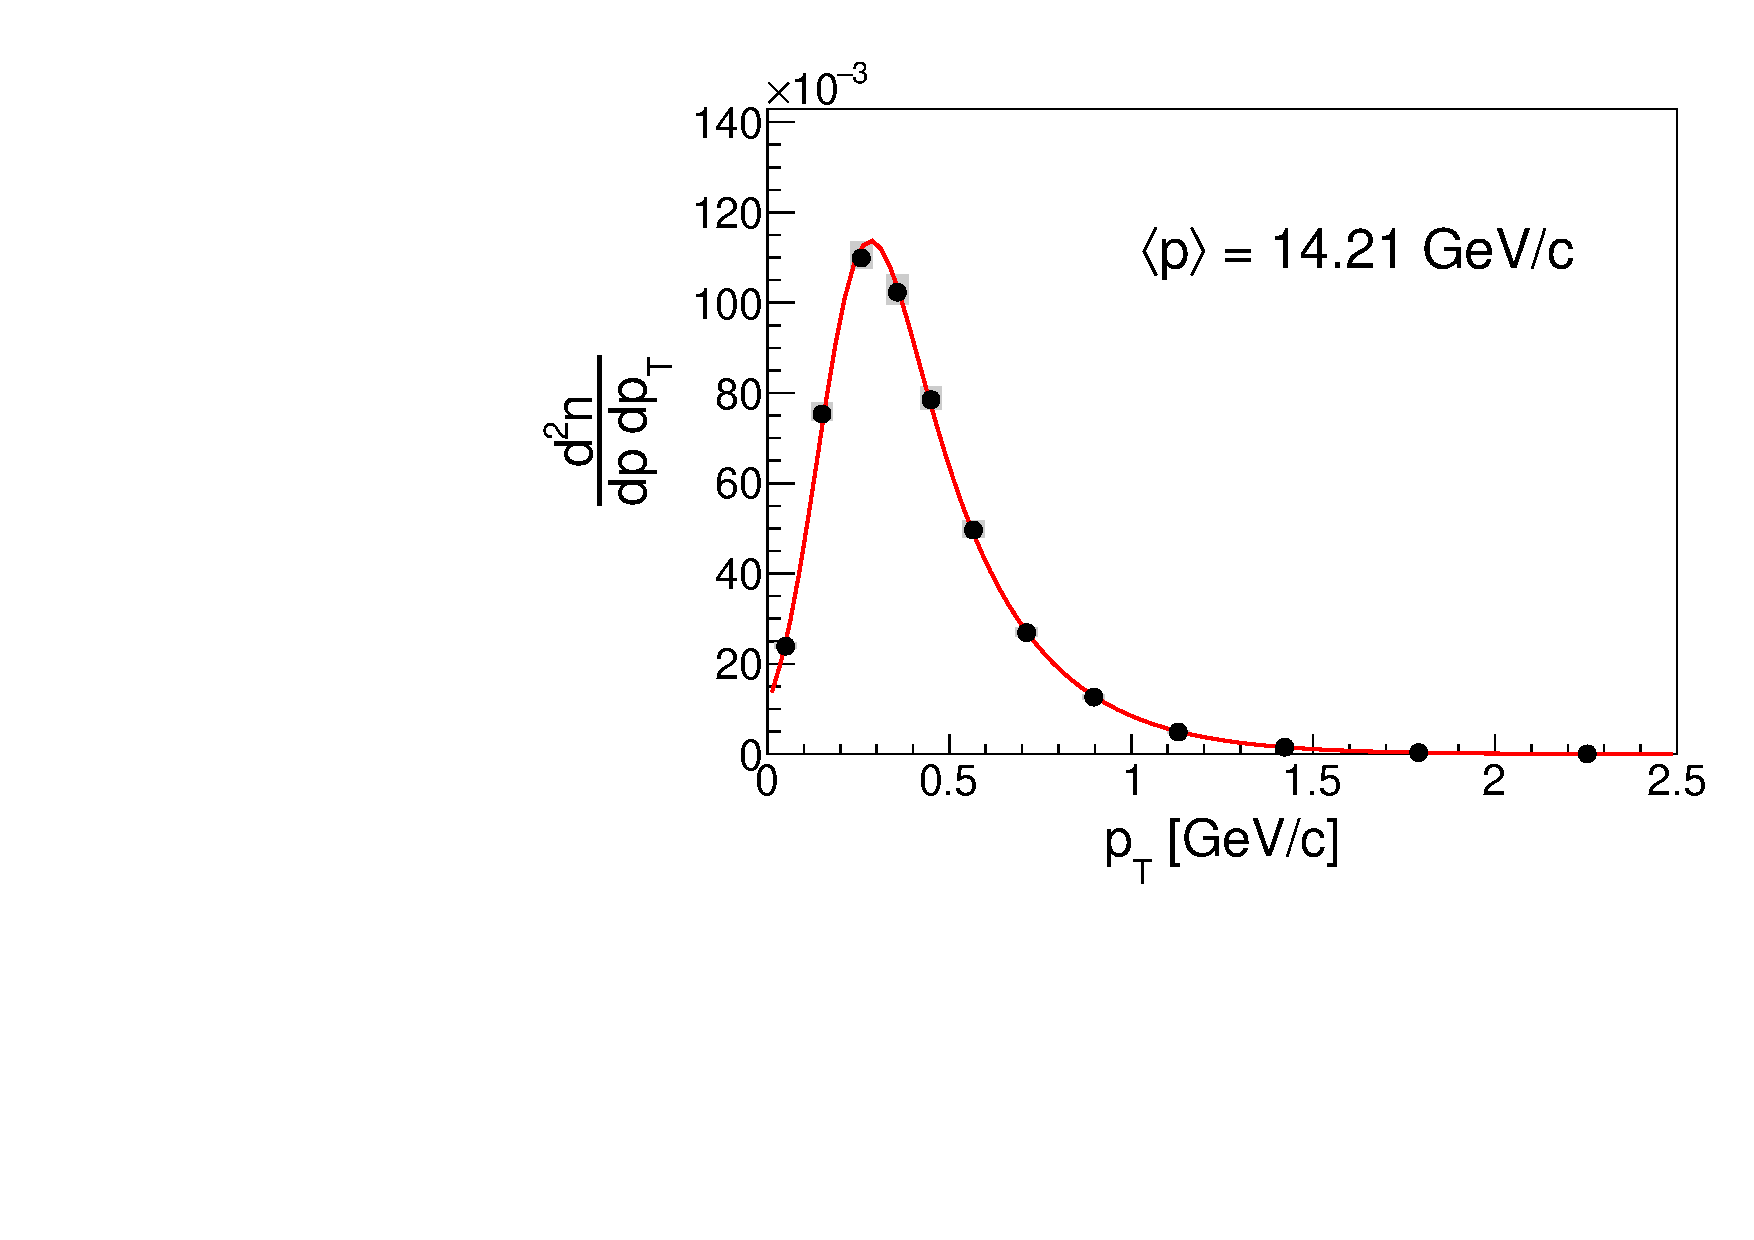
\includegraphics[clip, rviewport=0 0 1 1,width=0.24\textwidth]{spec/spec_pt_158_c1_p1_x22}
  \includegraphics[clip, rviewport=0 0 1 1,width=0.24\textwidth]{spec/spec_pt_158_c1_p1_x23}
  \includegraphics[clip, rviewport=0 0 1 1,width=0.24\textwidth]{spec/spec_pt_158_c1_p1_x24}

  \includegraphics[clip, rviewport=0 0 1 1,width=0.24\textwidth]{spec/spec_pt_158_c1_p1_x25}
  \includegraphics[clip, rviewport=0 0 1 1,width=0.24\textwidth]{spec/spec_pt_158_c1_p1_x26}
  \includegraphics[clip, rviewport=0 0 1 1,width=0.24\textwidth]{spec/spec_pt_158_c1_p1_x27}
  \includegraphics[clip, rviewport=0 0 1 1,width=0.24\textwidth]{spec/spec_pt_158_c1_p1_x28}

  \includegraphics[clip, rviewport=0 0 1 1,width=0.24\textwidth]{spec/spec_pt_158_c1_p1_x29}
  \includegraphics[clip, rviewport=0 0 1 1,width=0.24\textwidth]{spec/spec_pt_158_c1_p1_x30}
  \includegraphics[clip, rviewport=0 0 1 1,width=0.24\textwidth]{spec/spec_pt_158_c1_p1_x31}

  \caption{Double-differential spectra $\frac{\text{d}^2n}{\text{d}\pp\text{d}\pT}$
    of $\pi^-$ for the 158 \GeVc data set. Each plot shows one \pp bins and the value
    of $\langle\pp\rangle$ is indicated inside it. The black lines show the statistical
    uncertainties, while the gray bands show the systematic ones.}
  \label{fig:hadron:spec:dedx:all158:c1p1}
\end{figure}

%%%%%%%%%% SPEC PT ALL DEDX %%%%%%%%%%%%%%
\begin{figure}[!ht]
  \centering

  \includegraphics[clip, rviewport=0 0 1 1,width=0.24\textwidth]{spec/spec_pt_158_c0_p2_x7}
  \includegraphics[clip, rviewport=0 0 1 1,width=0.24\textwidth]{spec/spec_pt_158_c0_p2_x8}
  \includegraphics[clip, rviewport=0 0 1 1,width=0.24\textwidth]{spec/spec_pt_158_c0_p2_x9}
  \includegraphics[clip, rviewport=0 0 1 1,width=0.24\textwidth]{spec/spec_pt_158_c0_p2_x12}

  \includegraphics[clip, rviewport=0 0 1 1,width=0.24\textwidth]{spec/spec_pt_158_c0_p2_x13}
  \includegraphics[clip, rviewport=0 0 1 1,width=0.24\textwidth]{spec/spec_pt_158_c0_p2_x17}
  \includegraphics[clip, rviewport=0 0 1 1,width=0.24\textwidth]{spec/spec_pt_158_c0_p2_x18}
  \includegraphics[clip, rviewport=0 0 1 1,width=0.24\textwidth]{spec/spec_pt_158_c0_p2_x19}

  \includegraphics[clip, rviewport=0 0 1 1,width=0.24\textwidth]{spec/spec_pt_158_c0_p2_x20}
  \includegraphics[clip, rviewport=0 0 1 1,width=0.24\textwidth]{spec/spec_pt_158_c0_p2_x21}
  \includegraphics[clip, rviewport=0 0 1 1,width=0.24\textwidth]{spec/spec_pt_158_c0_p2_x22}
  \includegraphics[clip, rviewport=0 0 1 1,width=0.24\textwidth]{spec/spec_pt_158_c0_p2_x23}

  \includegraphics[clip, rviewport=0 0 1 1,width=0.24\textwidth]{spec/spec_pt_158_c0_p2_x24}
  \includegraphics[clip, rviewport=0 0 1 1,width=0.24\textwidth]{spec/spec_pt_158_c0_p2_x25}
  \includegraphics[clip, rviewport=0 0 1 1,width=0.24\textwidth]{spec/spec_pt_158_c0_p2_x26}
  \includegraphics[clip, rviewport=0 0 1 1,width=0.24\textwidth]{spec/spec_pt_158_c0_p2_x27}

  \includegraphics[clip, rviewport=0 0 1 1,width=0.24\textwidth]{spec/spec_pt_158_c0_p2_x28}
  \includegraphics[clip, rviewport=0 0 1 1,width=0.24\textwidth]{spec/spec_pt_158_c0_p2_x29}

  \caption{Double-differential spectra $\frac{\text{d}^2n}{\text{d}\pp\text{d}\pT}$
    of K$^+$ for the 158 \GeVc data set. Each plot shows one \pp bins and the value
    of $\langle\pp\rangle$ is indicated inside it. The black lines show the statistical
    uncertainties, while the gray bands show the systematic ones.}
  \label{fig:hadron:spec:dedx:all158:c0p2}
\end{figure}

%%%%%%%%%% SPEC PT ALL DEDX %%%%%%%%%%%%%%
\begin{figure}[!ht]
  \centering

  \includegraphics[clip, rviewport=0 0 1 1,width=0.24\textwidth]{spec/spec_pt_158_c1_p2_x8}
  \includegraphics[clip, rviewport=0 0 1 1,width=0.24\textwidth]{spec/spec_pt_158_c1_p2_x12}
  \includegraphics[clip, rviewport=0 0 1 1,width=0.24\textwidth]{spec/spec_pt_158_c1_p2_x13}
  \includegraphics[clip, rviewport=0 0 1 1,width=0.24\textwidth]{spec/spec_pt_158_c1_p2_x16}
  
  \includegraphics[clip, rviewport=0 0 1 1,width=0.24\textwidth]{spec/spec_pt_158_c1_p2_x17}
  \includegraphics[clip, rviewport=0 0 1 1,width=0.24\textwidth]{spec/spec_pt_158_c1_p2_x18}
  \includegraphics[clip, rviewport=0 0 1 1,width=0.24\textwidth]{spec/spec_pt_158_c1_p2_x19}
  \includegraphics[clip, rviewport=0 0 1 1,width=0.24\textwidth]{spec/spec_pt_158_c1_p2_x20}

  \includegraphics[clip, rviewport=0 0 1 1,width=0.24\textwidth]{spec/spec_pt_158_c1_p2_x21}
  \includegraphics[clip, rviewport=0 0 1 1,width=0.24\textwidth]{spec/spec_pt_158_c1_p2_x22}
  \includegraphics[clip, rviewport=0 0 1 1,width=0.24\textwidth]{spec/spec_pt_158_c1_p2_x23}
  \includegraphics[clip, rviewport=0 0 1 1,width=0.24\textwidth]{spec/spec_pt_158_c1_p2_x24}

  \includegraphics[clip, rviewport=0 0 1 1,width=0.24\textwidth]{spec/spec_pt_158_c1_p2_x25}
  \includegraphics[clip, rviewport=0 0 1 1,width=0.24\textwidth]{spec/spec_pt_158_c1_p2_x26}
  \includegraphics[clip, rviewport=0 0 1 1,width=0.24\textwidth]{spec/spec_pt_158_c1_p2_x27}
  \includegraphics[clip, rviewport=0 0 1 1,width=0.24\textwidth]{spec/spec_pt_158_c1_p2_x28}

  \includegraphics[clip, rviewport=0 0 1 1,width=0.24\textwidth]{spec/spec_pt_158_c1_p2_x29}

  \caption{Double-differential spectra $\frac{\text{d}^2n}{\text{d}\pp\text{d}\pT}$
    of K$^-$ for the 158 \GeVc data set. Each plot shows one \pp bins and the value
    of $\langle\pp\rangle$ is indicated inside it. The black lines show the statistical
    uncertainties, while the gray bands show the systematic ones.}
  \label{fig:hadron:spec:dedx:all158:c1p2}
\end{figure}

%%%%%%%%%% SPEC PT ALL DEDX %%%%%%%%%%%%%%
\begin{figure}[!ht]
  \centering

  \includegraphics[clip, rviewport=0 0 1 1,width=0.24\textwidth]{spec/spec_pt_158_c0_p3_x7}
  \includegraphics[clip, rviewport=0 0 1 1,width=0.24\textwidth]{spec/spec_pt_158_c0_p3_x8}
  \includegraphics[clip, rviewport=0 0 1 1,width=0.24\textwidth]{spec/spec_pt_158_c0_p3_x9}
  \includegraphics[clip, rviewport=0 0 1 1,width=0.24\textwidth]{spec/spec_pt_158_c0_p3_x10}

  \includegraphics[clip, rviewport=0 0 1 1,width=0.24\textwidth]{spec/spec_pt_158_c0_p3_x11}
  \includegraphics[clip, rviewport=0 0 1 1,width=0.24\textwidth]{spec/spec_pt_158_c0_p3_x13}
  \includegraphics[clip, rviewport=0 0 1 1,width=0.24\textwidth]{spec/spec_pt_158_c0_p3_x15}
  \includegraphics[clip, rviewport=0 0 1 1,width=0.24\textwidth]{spec/spec_pt_158_c0_p3_x16}

  \includegraphics[clip, rviewport=0 0 1 1,width=0.24\textwidth]{spec/spec_pt_158_c0_p3_x17}
  \includegraphics[clip, rviewport=0 0 1 1,width=0.24\textwidth]{spec/spec_pt_158_c0_p3_x18}
  \includegraphics[clip, rviewport=0 0 1 1,width=0.24\textwidth]{spec/spec_pt_158_c0_p3_x19}
  \includegraphics[clip, rviewport=0 0 1 1,width=0.24\textwidth]{spec/spec_pt_158_c0_p3_x20}

  \includegraphics[clip, rviewport=0 0 1 1,width=0.24\textwidth]{spec/spec_pt_158_c0_p3_x21}
  \includegraphics[clip, rviewport=0 0 1 1,width=0.24\textwidth]{spec/spec_pt_158_c0_p3_x22}
  \includegraphics[clip, rviewport=0 0 1 1,width=0.24\textwidth]{spec/spec_pt_158_c0_p3_x23}
  \includegraphics[clip, rviewport=0 0 1 1,width=0.24\textwidth]{spec/spec_pt_158_c0_p3_x24}

  \includegraphics[clip, rviewport=0 0 1 1,width=0.24\textwidth]{spec/spec_pt_158_c0_p3_x25}
  \includegraphics[clip, rviewport=0 0 1 1,width=0.24\textwidth]{spec/spec_pt_158_c0_p3_x26}
  \includegraphics[clip, rviewport=0 0 1 1,width=0.24\textwidth]{spec/spec_pt_158_c0_p3_x27}
  \includegraphics[clip, rviewport=0 0 1 1,width=0.24\textwidth]{spec/spec_pt_158_c0_p3_x28}

  \includegraphics[clip, rviewport=0 0 1 1,width=0.24\textwidth]{spec/spec_pt_158_c0_p3_x29}
  \includegraphics[clip, rviewport=0 0 1 1,width=0.24\textwidth]{spec/spec_pt_158_c0_p3_x30}

  \caption{Double-differential spectra $\frac{\text{d}^2n}{\text{d}\pp\text{d}\pT}$
    of p$^+$ for the 158 \GeVc data set. Each plot shows one \pp bins and the value
    of $\langle\pp\rangle$ is indicated inside it. The black lines show the statistical
    uncertainties, while the gray bands show the systematic ones.}
  \label{fig:hadron:spec:dedx:all158:c0p3}
\end{figure}

%%%%%%%%%% SPEC PT ALL DEDX %%%%%%%%%%%%%%
\begin{figure}[!ht]
  \centering

  \includegraphics[clip, rviewport=0 0 1 1,width=0.24\textwidth]{spec/spec_pt_158_c0_p3_x16}
  \includegraphics[clip, rviewport=0 0 1 1,width=0.24\textwidth]{spec/spec_pt_158_c0_p3_x17}
  \includegraphics[clip, rviewport=0 0 1 1,width=0.24\textwidth]{spec/spec_pt_158_c0_p3_x18}
  \includegraphics[clip, rviewport=0 0 1 1,width=0.24\textwidth]{spec/spec_pt_158_c0_p3_x19}

  \includegraphics[clip, rviewport=0 0 1 1,width=0.24\textwidth]{spec/spec_pt_158_c0_p3_x20}
  \includegraphics[clip, rviewport=0 0 1 1,width=0.24\textwidth]{spec/spec_pt_158_c0_p3_x21}
  \includegraphics[clip, rviewport=0 0 1 1,width=0.24\textwidth]{spec/spec_pt_158_c0_p3_x22}
  \includegraphics[clip, rviewport=0 0 1 1,width=0.24\textwidth]{spec/spec_pt_158_c0_p3_x23}

  \includegraphics[clip, rviewport=0 0 1 1,width=0.24\textwidth]{spec/spec_pt_158_c0_p3_x24}
  \includegraphics[clip, rviewport=0 0 1 1,width=0.24\textwidth]{spec/spec_pt_158_c0_p3_x25}
  \includegraphics[clip, rviewport=0 0 1 1,width=0.24\textwidth]{spec/spec_pt_158_c0_p3_x26}
  \includegraphics[clip, rviewport=0 0 1 1,width=0.24\textwidth]{spec/spec_pt_158_c0_p3_x27}

  \includegraphics[clip, rviewport=0 0 1 1,width=0.24\textwidth]{spec/spec_pt_158_c0_p3_x28}
  \includegraphics[clip, rviewport=0 0 1 1,width=0.24\textwidth]{spec/spec_pt_158_c0_p3_x29}
  \includegraphics[clip, rviewport=0 0 1 1,width=0.24\textwidth]{spec/spec_pt_158_c0_p3_x30}

  \caption{Double-differential spectra $\frac{\text{d}^2n}{\text{d}\pp\text{d}\pT}$
    of p$^-$ for the 158 \GeVc data set. Each plot shows one \pp bins and the value
    of $\langle\pp\rangle$ is indicated inside it. The black lines show the statistical
    uncertainties, while the gray bands show the systematic ones.}
  \label{fig:hadron:spec:dedx:all158:c1p3}
\end{figure}


%%%%%%%%%% SPEC PT ALL DEDX %%%%%%%%%%%%%%
\begin{figure}[!ht]
  \centering

  \includegraphics[clip, rviewport=0 0 1 1,width=0.24\textwidth]{spec/spec_pt_350_c0_p1_x7}
  \includegraphics[clip, rviewport=0 0 1 1,width=0.24\textwidth]{spec/spec_pt_350_c0_p1_x8}
  \includegraphics[clip, rviewport=0 0 1 1,width=0.24\textwidth]{spec/spec_pt_350_c0_p1_x9}
  \includegraphics[clip, rviewport=0 0 1 1,width=0.24\textwidth]{spec/spec_pt_350_c0_p1_x11}

  \includegraphics[clip, rviewport=0 0 1 1,width=0.24\textwidth]{spec/spec_pt_350_c0_p1_x13}
  \includegraphics[clip, rviewport=0 0 1 1,width=0.24\textwidth]{spec/spec_pt_350_c0_p1_x14}
  \includegraphics[clip, rviewport=0 0 1 1,width=0.24\textwidth]{spec/spec_pt_350_c0_p1_x15}
  \includegraphics[clip, rviewport=0 0 1 1,width=0.24\textwidth]{spec/spec_pt_350_c0_p1_x16}

  \includegraphics[clip, rviewport=0 0 1 1,width=0.24\textwidth]{spec/spec_pt_350_c0_p1_x17}
  \includegraphics[clip, rviewport=0 0 1 1,width=0.24\textwidth]{spec/spec_pt_350_c0_p1_x18}
  \includegraphics[clip, rviewport=0 0 1 1,width=0.24\textwidth]{spec/spec_pt_350_c0_p1_x19}
  \includegraphics[clip, rviewport=0 0 1 1,width=0.24\textwidth]{spec/spec_pt_350_c0_p1_x20}

  \includegraphics[clip, rviewport=0 0 1 1,width=0.24\textwidth]{spec/spec_pt_350_c0_p1_x21}
  \includegraphics[clip, rviewport=0 0 1 1,width=0.24\textwidth]{spec/spec_pt_350_c0_p1_x22}
  \includegraphics[clip, rviewport=0 0 1 1,width=0.24\textwidth]{spec/spec_pt_350_c0_p1_x23}
  \includegraphics[clip, rviewport=0 0 1 1,width=0.24\textwidth]{spec/spec_pt_350_c0_p1_x24}

  \includegraphics[clip, rviewport=0 0 1 1,width=0.24\textwidth]{spec/spec_pt_350_c0_p1_x25}
  \includegraphics[clip, rviewport=0 0 1 1,width=0.24\textwidth]{spec/spec_pt_350_c0_p1_x26}
  \includegraphics[clip, rviewport=0 0 1 1,width=0.24\textwidth]{spec/spec_pt_350_c0_p1_x27}
  \includegraphics[clip, rviewport=0 0 1 1,width=0.24\textwidth]{spec/spec_pt_350_c0_p1_x28}

  \includegraphics[clip, rviewport=0 0 1 1,width=0.24\textwidth]{spec/spec_pt_350_c0_p1_x29}
  \includegraphics[clip, rviewport=0 0 1 1,width=0.24\textwidth]{spec/spec_pt_350_c0_p1_x30}
  \includegraphics[clip, rviewport=0 0 1 1,width=0.24\textwidth]{spec/spec_pt_350_c0_p1_x31}

  \caption{Double-differential spectra $\frac{\text{d}^2n}{\text{d}\pp\text{d}\pT}$
    of $\pi^+$ for the 350 \GeVc data set. Each plot shows one \pp bins and the value
    of $\langle\pp\rangle$ is indicated inside it. The black lines show the statistical
    uncertainties, while the gray bands show the systematic ones.}
  \label{fig:hadron:spec:dedx:all350:c0p1}
\end{figure}


%%%%%%%%%% SPEC PT ALL DEDX %%%%%%%%%%%%%%
\begin{figure}[!ht]
  \centering

  \includegraphics[clip, rviewport=0 0 1 1,width=0.24\textwidth]{spec/spec_pt_350_c1_p1_x7}
  \includegraphics[clip, rviewport=0 0 1 1,width=0.24\textwidth]{spec/spec_pt_350_c1_p1_x8}
  \includegraphics[clip, rviewport=0 0 1 1,width=0.24\textwidth]{spec/spec_pt_350_c1_p1_x9}
  \includegraphics[clip, rviewport=0 0 1 1,width=0.24\textwidth]{spec/spec_pt_350_c1_p1_x11}

  \includegraphics[clip, rviewport=0 0 1 1,width=0.24\textwidth]{spec/spec_pt_350_c1_p1_x13}
  \includegraphics[clip, rviewport=0 0 1 1,width=0.24\textwidth]{spec/spec_pt_350_c1_p1_x14}
  \includegraphics[clip, rviewport=0 0 1 1,width=0.24\textwidth]{spec/spec_pt_350_c1_p1_x15}
  \includegraphics[clip, rviewport=0 0 1 1,width=0.24\textwidth]{spec/spec_pt_350_c1_p1_x16}

  \includegraphics[clip, rviewport=0 0 1 1,width=0.24\textwidth]{spec/spec_pt_350_c1_p1_x17}
  \includegraphics[clip, rviewport=0 0 1 1,width=0.24\textwidth]{spec/spec_pt_350_c1_p1_x18}
  \includegraphics[clip, rviewport=0 0 1 1,width=0.24\textwidth]{spec/spec_pt_350_c1_p1_x19}
  \includegraphics[clip, rviewport=0 0 1 1,width=0.24\textwidth]{spec/spec_pt_350_c1_p1_x20}

  \includegraphics[clip, rviewport=0 0 1 1,width=0.24\textwidth]{spec/spec_pt_350_c1_p1_x21}
  \includegraphics[clip, rviewport=0 0 1 1,width=0.24\textwidth]{spec/spec_pt_350_c1_p1_x22}
  \includegraphics[clip, rviewport=0 0 1 1,width=0.24\textwidth]{spec/spec_pt_350_c1_p1_x23}
  \includegraphics[clip, rviewport=0 0 1 1,width=0.24\textwidth]{spec/spec_pt_350_c1_p1_x24}

  \includegraphics[clip, rviewport=0 0 1 1,width=0.24\textwidth]{spec/spec_pt_350_c1_p1_x25}
  \includegraphics[clip, rviewport=0 0 1 1,width=0.24\textwidth]{spec/spec_pt_350_c1_p1_x26}
  \includegraphics[clip, rviewport=0 0 1 1,width=0.24\textwidth]{spec/spec_pt_350_c1_p1_x27}
  \includegraphics[clip, rviewport=0 0 1 1,width=0.24\textwidth]{spec/spec_pt_350_c1_p1_x28}

  \includegraphics[clip, rviewport=0 0 1 1,width=0.24\textwidth]{spec/spec_pt_350_c1_p1_x29}
  \includegraphics[clip, rviewport=0 0 1 1,width=0.24\textwidth]{spec/spec_pt_350_c1_p1_x30}
  \includegraphics[clip, rviewport=0 0 1 1,width=0.24\textwidth]{spec/spec_pt_350_c1_p1_x31}

  \caption{Double-differential spectra $\frac{\text{d}^2n}{\text{d}\pp\text{d}\pT}$
    of $\pi^-$ for the 350 \GeVc data set. Each plot shows one \pp bins and the value
    of $\langle\pp\rangle$ is indicated inside it. The black lines show the statistical
    uncertainties, while the gray bands show the systematic ones.}
  \label{fig:hadron:spec:dedx:all350:c1p1}
\end{figure}


%%%%%%%%%% SPEC PT ALL DEDX %%%%%%%%%%%%%%
\begin{figure}[!ht]
  \centering

  \includegraphics[clip, rviewport=0 0 1 1,width=0.24\textwidth]{spec/spec_pt_350_c0_p2_x8}
  \includegraphics[clip, rviewport=0 0 1 1,width=0.24\textwidth]{spec/spec_pt_350_c0_p2_x9}
  \includegraphics[clip, rviewport=0 0 1 1,width=0.24\textwidth]{spec/spec_pt_350_c0_p2_x12}
  \includegraphics[clip, rviewport=0 0 1 1,width=0.24\textwidth]{spec/spec_pt_350_c0_p2_x13}

  \includegraphics[clip, rviewport=0 0 1 1,width=0.24\textwidth]{spec/spec_pt_350_c0_p2_x17}
  \includegraphics[clip, rviewport=0 0 1 1,width=0.24\textwidth]{spec/spec_pt_350_c0_p2_x18}
  \includegraphics[clip, rviewport=0 0 1 1,width=0.24\textwidth]{spec/spec_pt_350_c0_p2_x19}
  \includegraphics[clip, rviewport=0 0 1 1,width=0.24\textwidth]{spec/spec_pt_350_c0_p2_x20}

  \includegraphics[clip, rviewport=0 0 1 1,width=0.24\textwidth]{spec/spec_pt_350_c0_p2_x21}
  \includegraphics[clip, rviewport=0 0 1 1,width=0.24\textwidth]{spec/spec_pt_350_c0_p2_x22}
  \includegraphics[clip, rviewport=0 0 1 1,width=0.24\textwidth]{spec/spec_pt_350_c0_p2_x23}
  \includegraphics[clip, rviewport=0 0 1 1,width=0.24\textwidth]{spec/spec_pt_350_c0_p2_x24}

  \includegraphics[clip, rviewport=0 0 1 1,width=0.24\textwidth]{spec/spec_pt_350_c0_p2_x25}
  \includegraphics[clip, rviewport=0 0 1 1,width=0.24\textwidth]{spec/spec_pt_350_c0_p2_x26}
  \includegraphics[clip, rviewport=0 0 1 1,width=0.24\textwidth]{spec/spec_pt_350_c0_p2_x27}
  \includegraphics[clip, rviewport=0 0 1 1,width=0.24\textwidth]{spec/spec_pt_350_c0_p2_x28}

  \includegraphics[clip, rviewport=0 0 1 1,width=0.24\textwidth]{spec/spec_pt_350_c0_p2_x29}
 
  \caption{Double-differential spectra $\frac{\text{d}^2n}{\text{d}\pp\text{d}\pT}$
    of K$^+$ for the 350 \GeVc data set. Each plot shows one \pp bins and the value
    of $\langle\pp\rangle$ is indicated inside it. The black lines show the statistical
    uncertainties, while the gray bands show the systematic ones.}
  \label{fig:hadron:spec:dedx:all350:c0p2}
\end{figure}

%%%%%%%%%% SPEC PT ALL DEDX %%%%%%%%%%%%%%
\begin{figure}[!ht]
  \centering

  \includegraphics[clip, rviewport=0 0 1 1,width=0.24\textwidth]{spec/spec_pt_350_c1_p2_x8}
  \includegraphics[clip, rviewport=0 0 1 1,width=0.24\textwidth]{spec/spec_pt_350_c1_p2_x12}
  \includegraphics[clip, rviewport=0 0 1 1,width=0.24\textwidth]{spec/spec_pt_350_c1_p2_x13}
  \includegraphics[clip, rviewport=0 0 1 1,width=0.24\textwidth]{spec/spec_pt_350_c1_p2_x16}

  \includegraphics[clip, rviewport=0 0 1 1,width=0.24\textwidth]{spec/spec_pt_350_c1_p2_x17}
  \includegraphics[clip, rviewport=0 0 1 1,width=0.24\textwidth]{spec/spec_pt_350_c1_p2_x18}
  \includegraphics[clip, rviewport=0 0 1 1,width=0.24\textwidth]{spec/spec_pt_350_c1_p2_x19}
  \includegraphics[clip, rviewport=0 0 1 1,width=0.24\textwidth]{spec/spec_pt_350_c1_p2_x20}

  \includegraphics[clip, rviewport=0 0 1 1,width=0.24\textwidth]{spec/spec_pt_350_c1_p2_x21}
  \includegraphics[clip, rviewport=0 0 1 1,width=0.24\textwidth]{spec/spec_pt_350_c1_p2_x22}
  \includegraphics[clip, rviewport=0 0 1 1,width=0.24\textwidth]{spec/spec_pt_350_c1_p2_x23}
  \includegraphics[clip, rviewport=0 0 1 1,width=0.24\textwidth]{spec/spec_pt_350_c1_p2_x24}

  \includegraphics[clip, rviewport=0 0 1 1,width=0.24\textwidth]{spec/spec_pt_350_c1_p2_x25}
  \includegraphics[clip, rviewport=0 0 1 1,width=0.24\textwidth]{spec/spec_pt_350_c1_p2_x26}
  \includegraphics[clip, rviewport=0 0 1 1,width=0.24\textwidth]{spec/spec_pt_350_c1_p2_x27}
  \includegraphics[clip, rviewport=0 0 1 1,width=0.24\textwidth]{spec/spec_pt_350_c1_p2_x28}

  \includegraphics[clip, rviewport=0 0 1 1,width=0.24\textwidth]{spec/spec_pt_350_c1_p2_x29}
 
 \caption{Double-differential spectra $\frac{\text{d}^2n}{\text{d}\pp\text{d}\pT}$
    of K$^-$ for the 350 \GeVc data set. Each plot shows one \pp bins and the value
    of $\langle\pp\rangle$ is indicated inside it. The black lines show the statistical
    uncertainties, while the gray bands show the systematic ones.}
  \label{fig:hadron:spec:dedx:all350:c1p2}
\end{figure}

%%%%%%%%%% SPEC PT ALL DEDX %%%%%%%%%%%%%%
\begin{figure}[!ht]
  \centering

  \includegraphics[clip, rviewport=0 0 1 1,width=0.24\textwidth]{spec/spec_pt_350_c0_p3_x7}
  \includegraphics[clip, rviewport=0 0 1 1,width=0.24\textwidth]{spec/spec_pt_350_c0_p3_x8}
  \includegraphics[clip, rviewport=0 0 1 1,width=0.24\textwidth]{spec/spec_pt_350_c0_p3_x9}
  \includegraphics[clip, rviewport=0 0 1 1,width=0.24\textwidth]{spec/spec_pt_350_c0_p3_x10}

  \includegraphics[clip, rviewport=0 0 1 1,width=0.24\textwidth]{spec/spec_pt_350_c0_p3_x11}
  \includegraphics[clip, rviewport=0 0 1 1,width=0.24\textwidth]{spec/spec_pt_350_c0_p3_x13}
  \includegraphics[clip, rviewport=0 0 1 1,width=0.24\textwidth]{spec/spec_pt_350_c0_p3_x15}
  \includegraphics[clip, rviewport=0 0 1 1,width=0.24\textwidth]{spec/spec_pt_350_c0_p3_x16}

  \includegraphics[clip, rviewport=0 0 1 1,width=0.24\textwidth]{spec/spec_pt_350_c0_p3_x17}
  \includegraphics[clip, rviewport=0 0 1 1,width=0.24\textwidth]{spec/spec_pt_350_c0_p3_x18}
  \includegraphics[clip, rviewport=0 0 1 1,width=0.24\textwidth]{spec/spec_pt_350_c0_p3_x19}
  \includegraphics[clip, rviewport=0 0 1 1,width=0.24\textwidth]{spec/spec_pt_350_c0_p3_x20}

  \includegraphics[clip, rviewport=0 0 1 1,width=0.24\textwidth]{spec/spec_pt_350_c0_p3_x21}
  \includegraphics[clip, rviewport=0 0 1 1,width=0.24\textwidth]{spec/spec_pt_350_c0_p3_x22}
  \includegraphics[clip, rviewport=0 0 1 1,width=0.24\textwidth]{spec/spec_pt_350_c0_p3_x23}
  \includegraphics[clip, rviewport=0 0 1 1,width=0.24\textwidth]{spec/spec_pt_350_c0_p3_x24}

  \includegraphics[clip, rviewport=0 0 1 1,width=0.24\textwidth]{spec/spec_pt_350_c0_p3_x25}
  \includegraphics[clip, rviewport=0 0 1 1,width=0.24\textwidth]{spec/spec_pt_350_c0_p3_x26}
  \includegraphics[clip, rviewport=0 0 1 1,width=0.24\textwidth]{spec/spec_pt_350_c0_p3_x27}
  \includegraphics[clip, rviewport=0 0 1 1,width=0.24\textwidth]{spec/spec_pt_350_c0_p3_x28}

  \includegraphics[clip, rviewport=0 0 1 1,width=0.24\textwidth]{spec/spec_pt_350_c0_p3_x29}
  \includegraphics[clip, rviewport=0 0 1 1,width=0.24\textwidth]{spec/spec_pt_350_c0_p3_x30}
 
  \caption{Double-differential spectra $\frac{\text{d}^2n}{\text{d}\pp\text{d}\pT}$
    of p$^+$ for the 350 \GeVc data set. Each plot shows one \pp bins and the value
    of $\langle\pp\rangle$ is indicated inside it. The black lines show the statistical
    uncertainties, while the gray bands show the systematic ones.}
  \label{fig:hadron:spec:dedx:all350:c0p3}
\end{figure}

%%%%%%%%%% SPEC PT ALL DEDX %%%%%%%%%%%%%%
\begin{figure}[!ht]
  \centering

  \includegraphics[clip, rviewport=0 0 1 1,width=0.24\textwidth]{spec/spec_pt_350_c1_p3_x10}
  \includegraphics[clip, rviewport=0 0 1 1,width=0.24\textwidth]{spec/spec_pt_350_c1_p3_x16}
  \includegraphics[clip, rviewport=0 0 1 1,width=0.24\textwidth]{spec/spec_pt_350_c1_p3_x17}
  \includegraphics[clip, rviewport=0 0 1 1,width=0.24\textwidth]{spec/spec_pt_350_c1_p3_x18}

  \includegraphics[clip, rviewport=0 0 1 1,width=0.24\textwidth]{spec/spec_pt_350_c1_p3_x19}
  \includegraphics[clip, rviewport=0 0 1 1,width=0.24\textwidth]{spec/spec_pt_350_c1_p3_x20}
  \includegraphics[clip, rviewport=0 0 1 1,width=0.24\textwidth]{spec/spec_pt_350_c1_p3_x21}
  \includegraphics[clip, rviewport=0 0 1 1,width=0.24\textwidth]{spec/spec_pt_350_c1_p3_x22}

  \includegraphics[clip, rviewport=0 0 1 1,width=0.24\textwidth]{spec/spec_pt_350_c1_p3_x23}
  \includegraphics[clip, rviewport=0 0 1 1,width=0.24\textwidth]{spec/spec_pt_350_c1_p3_x24}
  \includegraphics[clip, rviewport=0 0 1 1,width=0.24\textwidth]{spec/spec_pt_350_c1_p3_x25}
  \includegraphics[clip, rviewport=0 0 1 1,width=0.24\textwidth]{spec/spec_pt_350_c1_p3_x26}

  \includegraphics[clip, rviewport=0 0 1 1,width=0.24\textwidth]{spec/spec_pt_350_c1_p3_x27}
  \includegraphics[clip, rviewport=0 0 1 1,width=0.24\textwidth]{spec/spec_pt_350_c1_p3_x28}
  \includegraphics[clip, rviewport=0 0 1 1,width=0.24\textwidth]{spec/spec_pt_350_c1_p3_x29}
  \includegraphics[clip, rviewport=0 0 1 1,width=0.24\textwidth]{spec/spec_pt_350_c1_p3_x30}
 
  \caption{Double-differential spectra $\frac{\text{d}^2n}{\text{d}\pp\text{d}\pT}$
    of p$^-$ for the 350 \GeVc data set. Each plot shows one \pp bins and the value
    of $\langle\pp\rangle$ is indicated inside it. The black lines show the statistical
    uncertainties, while the gray bands show the systematic ones.}
  \label{fig:hadron:spec:dedx:all350:c1p3}
\end{figure}

\clearpage

%%%%%%%%%% SPEC PT ALL V0 %%%%%%%%%%%%%%
\begin{figure}[!ht]
  \centering

  \includegraphics[clip, rviewport=0 0 1 1,width=0.32\textwidth]{spec/spec_pt_158_h0_p1}
  \includegraphics[clip, rviewport=0 0 1 1,width=0.32\textwidth]{spec/spec_pt_158_h0_p2}
  \includegraphics[clip, rviewport=0 0 1 1,width=0.32\textwidth]{spec/spec_pt_158_h0_p3}

  \includegraphics[clip, rviewport=0 0 1 1,width=0.32\textwidth]{spec/spec_pt_158_h0_p4}
  \includegraphics[clip, rviewport=0 0 1 1,width=0.32\textwidth]{spec/spec_pt_158_h0_p5}
  \includegraphics[clip, rviewport=0 0 1 1,width=0.32\textwidth]{spec/spec_pt_158_h0_p6}

  \caption{}
  \label{fig:hadron:spec:vzero:all158:h0}
\end{figure}


%%%%%%%%%% SPEC PT ALL V0 %%%%%%%%%%%%%%
\begin{figure}[!ht]
  \centering

  \includegraphics[clip, rviewport=0 0 1 1,width=0.32\textwidth]{spec/spec_pt_158_h1_p1}
  \includegraphics[clip, rviewport=0 0 1 1,width=0.32\textwidth]{spec/spec_pt_158_h1_p2}
  \includegraphics[clip, rviewport=0 0 1 1,width=0.32\textwidth]{spec/spec_pt_158_h1_p3}

  \includegraphics[clip, rviewport=0 0 1 1,width=0.32\textwidth]{spec/spec_pt_158_h1_p4}
  \includegraphics[clip, rviewport=0 0 1 1,width=0.32\textwidth]{spec/spec_pt_158_h1_p5}
  \includegraphics[clip, rviewport=0 0 1 1,width=0.32\textwidth]{spec/spec_pt_158_h1_p6}

  \caption{}
  \label{fig:hadron:spec:vzero:all158:h1}
\end{figure}


%%%%%%%%%% SPEC PT ALL V0 %%%%%%%%%%%%%%
\begin{figure}[!ht]
  \centering

  \includegraphics[clip, rviewport=0 0 1 1,width=0.32\textwidth]{spec/spec_pt_158_h2_p0}
  \includegraphics[clip, rviewport=0 0 1 1,width=0.32\textwidth]{spec/spec_pt_158_h2_p1}
  \includegraphics[clip, rviewport=0 0 1 1,width=0.32\textwidth]{spec/spec_pt_158_h2_p2}
  
  \includegraphics[clip, rviewport=0 0 1 1,width=0.32\textwidth]{spec/spec_pt_158_h2_p3}
  \includegraphics[clip, rviewport=0 0 1 1,width=0.32\textwidth]{spec/spec_pt_158_h2_p4}
  \includegraphics[clip, rviewport=0 0 1 1,width=0.32\textwidth]{spec/spec_pt_158_h2_p5}

  \includegraphics[clip, rviewport=0 0 1 1,width=0.32\textwidth]{spec/spec_pt_158_h2_p6}
  \includegraphics[clip, rviewport=0 0 1 1,width=0.32\textwidth]{spec/spec_pt_158_h2_p7}
  \includegraphics[clip, rviewport=0 0 1 1,width=0.32\textwidth]{spec/spec_pt_158_h2_p8}

  \caption{}
  \label{fig:hadron:spec:vzero:all158:h2}
\end{figure}


%%%%%%%%%% SPEC PT ALL V0 %%%%%%%%%%%%%%
\begin{figure}[!ht]
  \centering

  \includegraphics[clip, rviewport=0 0 1 1,width=0.32\textwidth]{spec/spec_pt_350_h0_p1}
  \includegraphics[clip, rviewport=0 0 1 1,width=0.32\textwidth]{spec/spec_pt_350_h0_p2}
  \includegraphics[clip, rviewport=0 0 1 1,width=0.32\textwidth]{spec/spec_pt_350_h0_p3}

  \includegraphics[clip, rviewport=0 0 1 1,width=0.32\textwidth]{spec/spec_pt_350_h0_p4}
  \includegraphics[clip, rviewport=0 0 1 1,width=0.32\textwidth]{spec/spec_pt_350_h0_p5}
  \includegraphics[clip, rviewport=0 0 1 1,width=0.32\textwidth]{spec/spec_pt_350_h0_p6}

  \caption{}
  \label{fig:hadron:spec:vzero:all350:h0}
\end{figure}


%%%%%%%%%% SPEC PT ALL V0 %%%%%%%%%%%%%%
\begin{figure}[!ht]
  \centering

  \includegraphics[clip, rviewport=0 0 1 1,width=0.32\textwidth]{spec/spec_pt_350_h1_p1}
  \includegraphics[clip, rviewport=0 0 1 1,width=0.32\textwidth]{spec/spec_pt_350_h1_p2}
  \includegraphics[clip, rviewport=0 0 1 1,width=0.32\textwidth]{spec/spec_pt_350_h1_p3}

  \includegraphics[clip, rviewport=0 0 1 1,width=0.32\textwidth]{spec/spec_pt_350_h1_p4}
  \includegraphics[clip, rviewport=0 0 1 1,width=0.32\textwidth]{spec/spec_pt_350_h1_p5}
  \includegraphics[clip, rviewport=0 0 1 1,width=0.32\textwidth]{spec/spec_pt_350_h1_p6}

  \caption{}
  \label{fig:hadron:spec:vzero:all350:h1}
\end{figure}


%%%%%%%%%% SPEC PT ALL V0 %%%%%%%%%%%%%%
\begin{figure}[!ht]
  \centering

  \includegraphics[clip, rviewport=0 0 1 1,width=0.32\textwidth]{spec/spec_pt_350_h2_p0}
  \includegraphics[clip, rviewport=0 0 1 1,width=0.32\textwidth]{spec/spec_pt_350_h2_p1}
  \includegraphics[clip, rviewport=0 0 1 1,width=0.32\textwidth]{spec/spec_pt_350_h2_p2}
  
  \includegraphics[clip, rviewport=0 0 1 1,width=0.32\textwidth]{spec/spec_pt_350_h2_p3}
  \includegraphics[clip, rviewport=0 0 1 1,width=0.32\textwidth]{spec/spec_pt_350_h2_p4}
  \includegraphics[clip, rviewport=0 0 1 1,width=0.32\textwidth]{spec/spec_pt_350_h2_p5}

  \includegraphics[clip, rviewport=0 0 1 1,width=0.32\textwidth]{spec/spec_pt_350_h2_p6}
  \includegraphics[clip, rviewport=0 0 1 1,width=0.32\textwidth]{spec/spec_pt_350_h2_p7}
  \includegraphics[clip, rviewport=0 0 1 1,width=0.32\textwidth]{spec/spec_pt_350_h2_p8}

  \caption{}
  \label{fig:hadron:spec:vzero:all350:h2}
\end{figure}


\chapter[Conclusions]{Conclusions}
\label{sec:conclusions}


% ----------------------------------------------------------
% ELEMENTOS PÓS-TEXTUAIS
% ----------------------------------------------------------
\postextual
% ----------------------------------------------------------

% -----------------------------------------------------------
% Referências bibliográficas
% ----------------------------------------------------------
\bibliography{lib}

\addcontentsline{toc}{chapter}{APPENDIX}
\appendix
%\begin{appendices}
\chapter{Additional figures}
\clearpage

%%%%%%%%%%% DIST %%%%%%%%%%%%%%%%%%
\begin{figure}
  \centering

  \begin{overpic}[clip, rviewport=0 0 1 1,width=0.4\textwidth]{dedx/dist_350_v0_c0_x13_y3}
    \put(16,85){(a)}
  \end{overpic}
  \begin{overpic}[clip, rviewport=0 0 1 1,width=0.4\textwidth]{dedx/dist_350_v0_c1_x13_y3}
    \put(16,85){(b)}
  \end{overpic}

  \vspace{0.5cm}
  
  \begin{overpic}[clip, rviewport=0 0 1 1,width=0.4\textwidth]{dedx/dist_350_v1_c0_x29_y5}
    \put(16,85){(c)}
  \end{overpic}
  \begin{overpic}[clip, rviewport=0 0 1 1,width=0.4\textwidth]{dedx/dist_350_v1_c1_x29_y5}
    \put(16,85){(d)}
  \end{overpic}
  
  \caption{Examples of the fitted \dedx distributions from the 350 \GeVc dataset.
    On the top, the distributions of the (a) negatively and (b) positively charged
    tracks are shown for one phase space bin of the RST subset. On the bottom,
    the distributions of the (c) negatively and (d) positively charged
    tracks are shown for a different phase space bin of the WST subset.
    The values of the $\langle\pp\rangle$ and $\langle\pT\rangle$ for
    each phase space bin is indicated on the top of each plot.
    The black dots show the observed number of tracks, while the colored
    distributions are the results of the \dedx fit or each particle type. 
    On the bottom of each plot, we show the residual of the fit, defined
    as the difference between the observed and the expected number of tracks
    from the result of the fit, divided by the uncertainty of the observed number.}
  \label{fig:hadron:dedx:fit:dist350}
\end{figure}



%%%%%%%%%% CHI SQ %%%%%%%%%%%%%%
\begin{figure}
  \centering

  \begin{overpic}[clip, rviewport=0 0 1 0.945,width=0.4\textwidth]{dedx/chisq_350_v0}
    \put(18,58){(a)}
  \end{overpic}
  \begin{overpic}[clip, rviewport=0 0 1 0.945,width=0.4\textwidth]{dedx/chisq_350_v0}
    \put(18,58){(b)}
  \end{overpic}

  \caption{\redchisq of the \dedx fit for the 350 \GeVc data set.
    The RST and WST are shown in (a) and (b), respectively.}
  \label{fig:hadron:dedx:fit:chi350}
\end{figure}

%%%%%%%%%% CAL %%%%%%%%%%%%%%
\begin{figure}[!ht]
  \centering

  \begin{overpic}[clip, rviewport=0 0 1 0.94,width=0.49\textwidth]{dedx/model_158_v1_m0}
    \put(18,58){(a)}
  \end{overpic}
  \begin{overpic}[clip, rviewport=0 0 1 0.94,width=0.49\textwidth]{dedx/model_158_v1_m1}
    \put(18,58){(b)}
  \end{overpic}

  \begin{overpic}[clip, rviewport=0 0 1 0.94,width=0.49\textwidth]{dedx/model_158_v1_m2}
    \put(18,58){(c)}
  \end{overpic}
  \begin{overpic}[clip, rviewport=0 0 1 0.94,width=0.49\textwidth]{dedx/model_158_v1_m3}
    \put(18,58){(d)}
  \end{overpic}

  \begin{overpic}[clip, rviewport=0 0 1 0.94,width=0.49\textwidth]{dedx/model_158_v1_m4}
    \put(18,58){(e)}
  \end{overpic}
  \begin{overpic}[clip, rviewport=0 0 1 0.94,width=0.49\textwidth]{dedx/model_158_v1_m5}
    \put(18,58){(f)}
  \end{overpic}

  \caption{Calibration constants obtained from the \dedx fit of the WST and 158 \GeVc data set.}
  \label{fig:hadron:dedx:fit:cal158w}
\end{figure}

%%%%%%%%%% CAL %%%%%%%%%%%%%%
\begin{figure}[!ht]
  \centering

  \begin{overpic}[clip, rviewport=0 0 1 0.94,width=0.49\textwidth]{dedx/model_350_v0_m0}
    \put(18,58){(a)}
  \end{overpic}
  \begin{overpic}[clip, rviewport=0 0 1 0.94,width=0.49\textwidth]{dedx/model_350_v0_m1}
    \put(18,58){(b)}
  \end{overpic}

  \begin{overpic}[clip, rviewport=0 0 1 0.94,width=0.49\textwidth]{dedx/model_350_v0_m2}
    \put(18,58){(c)}
  \end{overpic}
  \begin{overpic}[clip, rviewport=0 0 1 0.94,width=0.49\textwidth]{dedx/model_350_v0_m3}
    \put(18,58){(d)}
  \end{overpic}

  \begin{overpic}[clip, rviewport=0 0 1 0.94,width=0.49\textwidth]{dedx/model_350_v0_m4}
    \put(18,58){(e)}
  \end{overpic}
  \begin{overpic}[clip, rviewport=0 0 1 0.94,width=0.49\textwidth]{dedx/model_350_v0_m5}
    \put(18,58){(f)}
  \end{overpic}

  \caption{Calibration constants obtained from the \dedx fit of the RST and 350 \GeVc data set.}
  \label{fig:hadron:dedx:fit:cal350r}
\end{figure}


%%%%%%%%%% CAL %%%%%%%%%%%%%%
\begin{figure}[!ht]
  \centering

  \begin{overpic}[clip, rviewport=0 0 1 0.94,width=0.49\textwidth]{dedx/model_350_v1_m0}
    \put(18,58){(a)}
  \end{overpic}
  \begin{overpic}[clip, rviewport=0 0 1 0.94,width=0.49\textwidth]{dedx/model_350_v1_m1}
    \put(18,58){(b)}
  \end{overpic}

  \begin{overpic}[clip, rviewport=0 0 1 0.94,width=0.49\textwidth]{dedx/model_350_v1_m2}
    \put(18,58){(c)}
  \end{overpic}
  \begin{overpic}[clip, rviewport=0 0 1 0.94,width=0.49\textwidth]{dedx/model_350_v1_m3}
    \put(18,58){(d)}
  \end{overpic}

  \begin{overpic}[clip, rviewport=0 0 1 0.94,width=0.49\textwidth]{dedx/model_350_v1_m4}
    \put(18,58){(e)}
  \end{overpic}
  \begin{overpic}[clip, rviewport=0 0 1 0.94,width=0.49\textwidth]{dedx/model_350_v1_m5}
    \put(18,58){(f)}
  \end{overpic}

  \caption{Calibration constants obtained from the \dedx fit of the WST and 350 \GeVc data set.}
  \label{fig:hadron:dedx:fit:cal350w}
\end{figure}

\clearpage

%%%%%%%%%% SHAPE %%%%%%%%%%%%%%
\begin{figure}[!ht]
  \centering

  \begin{overpic}[clip, rviewport=0 0 1 0.94,width=0.49\textwidth]{dedx/model_158_v1_m6}
    \put(18,58){(a)}
  \end{overpic}
  \begin{overpic}[clip, rviewport=0 0 1 0.94,width=0.49\textwidth]{dedx/model_158_v1_m7}
    \put(18,58){(b)}
  \end{overpic}

  \begin{overpic}[clip, rviewport=0 0 1 0.94,width=0.49\textwidth]{dedx/model_158_v1_m9}
    \put(18,58){(c)}
  \end{overpic}
  \begin{overpic}[clip, rviewport=0 0 1 0.94,width=0.49\textwidth]{dedx/model_158_v1_m10}
    \put(18,58){(d)}
  \end{overpic}

  \caption{Shape parameters obtained from the \dedx fit of the WST and 158 \GeVc data set.}
  \label{fig:hadron:dedx:fit:shape158w}
\end{figure}

%%%%%%%%%% SHAPE %%%%%%%%%%%%%%
\begin{figure}[!ht]
  \centering

  \begin{overpic}[clip, rviewport=0 0 1 0.94,width=0.49\textwidth]{dedx/model_350_v0_m6}
    \put(18,58){(a)}
  \end{overpic}
  \begin{overpic}[clip, rviewport=0 0 1 0.94,width=0.49\textwidth]{dedx/model_350_v0_m7}
    \put(18,58){(b)}
  \end{overpic}

  \begin{overpic}[clip, rviewport=0 0 1 0.94,width=0.49\textwidth]{dedx/model_350_v0_m9}
    \put(18,58){(c)}
  \end{overpic}
  \begin{overpic}[clip, rviewport=0 0 1 0.94,width=0.49\textwidth]{dedx/model_350_v0_m10}
    \put(18,58){(d)}
  \end{overpic}

  \caption{Shape parameters obtained from the \dedx fit of the RST and 350 \GeVc data set.}
  \label{fig:hadron:dedx:fit:shape350r}
\end{figure}

%%%%%%%%%% SHAPE %%%%%%%%%%%%%%
\begin{figure}[!ht]
  \centering

  \begin{overpic}[clip, rviewport=0 0 1 0.94,width=0.49\textwidth]{dedx/model_350_v1_m6}
    \put(18,58){(a)}
  \end{overpic}
  \begin{overpic}[clip, rviewport=0 0 1 0.94,width=0.49\textwidth]{dedx/model_350_v1_m7}
    \put(18,58){(b)}
  \end{overpic}

  \begin{overpic}[clip, rviewport=0 0 1 0.94,width=0.49\textwidth]{dedx/model_350_v1_m9}
    \put(18,58){(c)}
  \end{overpic}
  \begin{overpic}[clip, rviewport=0 0 1 0.94,width=0.49\textwidth]{dedx/model_350_v1_m10}
    \put(18,58){(d)}
  \end{overpic}

  \caption{Shape parameters obtained from the \dedx fit of the WST and 350 \GeVc data set.}
  \label{fig:hadron:dedx:fit:shape350w}
\end{figure}


\clearpage



%%%%%%%%%% FRACTIONS %%%%%%%%%%%%%%
\begin{figure}
  \centering

  \begin{overpic}[clip, rviewport=0 0.125 1 0.94,width=0.45\textwidth]{dedx/fraction_158_fl0_v1_c0_p0}
    \put(18,49){(a)}
  \end{overpic}
  \begin{overpic}[clip, rviewport=0 0.125 1 0.94,width=0.45\textwidth]{dedx/fraction_158_fl0_v1_c1_p0}
    \put(18,49){(b)}
  \end{overpic}

  \begin{overpic}[clip, rviewport=0 0.125 1 0.94,width=0.45\textwidth]{dedx/fraction_158_fl0_v1_c0_p1}
    \put(18,49){(c)}
  \end{overpic}
  \begin{overpic}[clip, rviewport=0 0.125 1 0.94,width=0.45\textwidth]{dedx/fraction_158_fl0_v1_c1_p1}
    \put(18,49){(d)}
  \end{overpic}

   \begin{overpic}[clip, rviewport=0 0.125 1 0.94,width=0.45\textwidth]{dedx/fraction_158_fl0_v1_c0_p2}
    \put(18,49){(e)}
  \end{overpic}
  \begin{overpic}[clip, rviewport=0 0.125 1 0.94,width=0.45\textwidth]{dedx/fraction_158_fl0_v1_c1_p2}
    \put(18,49){(f)}
  \end{overpic}

   \begin{overpic}[clip, rviewport=0 0.125 1 0.94,width=0.45\textwidth]{dedx/fraction_158_fl0_v1_c0_p3}
    \put(18,49){(g)}
  \end{overpic}
  \begin{overpic}[clip, rviewport=0 0.125 1 0.94,width=0.45\textwidth]{dedx/fraction_158_fl0_v1_c1_p3}
    \put(18,49){(h)}
  \end{overpic}

   \begin{overpic}[clip, rviewport=0 0 1 0.94,width=0.45\textwidth]{dedx/fraction_158_fl0_v1_c0_p4}
    \put(18,58){(i)}
  \end{overpic}
  \begin{overpic}[clip, rviewport=0 0 1 0.94,width=0.45\textwidth]{dedx/fraction_158_fl0_v1_c1_p4}
    \put(18,58){(j)}
  \end{overpic}
  
  \caption{Particle fractions obtained from the \dedx fit of the WST and 158 \GeVc data set.}
  \label{fig:hadron:dedx:fit:frac158w}
\end{figure}


%%%%%%%%%% FRACTIONS %%%%%%%%%%%%%%
\begin{figure}
  \centering

  \begin{overpic}[clip, rviewport=0 0.125 1 0.94,width=0.45\textwidth]{dedx/fraction_350_fl0_v0_c0_p0}
    \put(18,49){(a)}
  \end{overpic}
  \begin{overpic}[clip, rviewport=0 0.125 1 0.94,width=0.45\textwidth]{dedx/fraction_350_fl0_v0_c1_p0}
    \put(18,49){(b)}
  \end{overpic}

  \begin{overpic}[clip, rviewport=0 0.125 1 0.94,width=0.45\textwidth]{dedx/fraction_350_fl0_v0_c0_p1}
    \put(18,49){(c)}
  \end{overpic}
  \begin{overpic}[clip, rviewport=0 0.125 1 0.94,width=0.45\textwidth]{dedx/fraction_350_fl0_v0_c1_p1}
    \put(18,49){(d)}
  \end{overpic}

   \begin{overpic}[clip, rviewport=0 0.125 1 0.94,width=0.45\textwidth]{dedx/fraction_350_fl0_v0_c0_p2}
    \put(18,49){(e)}
  \end{overpic}
  \begin{overpic}[clip, rviewport=0 0.125 1 0.94,width=0.45\textwidth]{dedx/fraction_350_fl0_v0_c1_p2}
    \put(18,49){(f)}
  \end{overpic}

   \begin{overpic}[clip, rviewport=0 0.125 1 0.94,width=0.45\textwidth]{dedx/fraction_350_fl0_v0_c0_p3}
    \put(18,49){(g)}
  \end{overpic}
  \begin{overpic}[clip, rviewport=0 0.125 1 0.94,width=0.45\textwidth]{dedx/fraction_350_fl0_v0_c1_p3}
    \put(18,49){(h)}
  \end{overpic}

   \begin{overpic}[clip, rviewport=0 0 1 0.94,width=0.45\textwidth]{dedx/fraction_350_fl0_v0_c0_p4}
    \put(18,58){(i)}
  \end{overpic}
  \begin{overpic}[clip, rviewport=0 0 1 0.94,width=0.45\textwidth]{dedx/fraction_350_fl0_v0_c1_p4}
    \put(18,58){(j)}
  \end{overpic}
  
  \caption{Particle fractions obtained from the \dedx fit of the RST and 350 \GeVc data set.}
  \label{fig:hadron:dedx:fit:frac350r}
\end{figure}


%%%%%%%%%% FRACTIONS %%%%%%%%%%%%%%
\begin{figure}
  \centering

  \begin{overpic}[clip, rviewport=0 0.125 1 0.94,width=0.45\textwidth]{dedx/fraction_350_fl0_v1_c0_p0}
    \put(18,49){(a)}
  \end{overpic}
  \begin{overpic}[clip, rviewport=0 0.125 1 0.94,width=0.45\textwidth]{dedx/fraction_350_fl0_v1_c1_p0}
    \put(18,49){(b)}
  \end{overpic}

  \begin{overpic}[clip, rviewport=0 0.125 1 0.94,width=0.45\textwidth]{dedx/fraction_350_fl0_v1_c0_p1}
    \put(18,49){(c)}
  \end{overpic}
  \begin{overpic}[clip, rviewport=0 0.125 1 0.94,width=0.45\textwidth]{dedx/fraction_350_fl0_v1_c1_p1}
    \put(18,49){(d)}
  \end{overpic}

   \begin{overpic}[clip, rviewport=0 0.125 1 0.94,width=0.45\textwidth]{dedx/fraction_350_fl0_v1_c0_p2}
    \put(18,49){(e)}
  \end{overpic}
  \begin{overpic}[clip, rviewport=0 0.125 1 0.94,width=0.45\textwidth]{dedx/fraction_350_fl0_v1_c1_p2}
    \put(18,49){(f)}
  \end{overpic}

   \begin{overpic}[clip, rviewport=0 0.125 1 0.94,width=0.45\textwidth]{dedx/fraction_350_fl0_v1_c0_p3}
    \put(18,49){(g)}
  \end{overpic}
  \begin{overpic}[clip, rviewport=0 0.125 1 0.94,width=0.45\textwidth]{dedx/fraction_350_fl0_v1_c1_p3}
    \put(18,49){(h)}
  \end{overpic}

   \begin{overpic}[clip, rviewport=0 0 1 0.94,width=0.45\textwidth]{dedx/fraction_350_fl0_v1_c0_p4}
    \put(18,58){(i)}
  \end{overpic}
  \begin{overpic}[clip, rviewport=0 0 1 0.94,width=0.45\textwidth]{dedx/fraction_350_fl0_v1_c1_p4}
    \put(18,58){(j)}
  \end{overpic}
  
  \caption{Particle fractions obtained from the \dedx fit of the WST and 350 \GeVc data set.}
  \label{fig:hadron:dedx:fit:frac350w}
\end{figure}

\clearpage

%%%%%%%%%% FAKE REL SIG %%%%%%%%%%%%%%
\begin{figure}[!ht]
  \centering
  
  \begin{overpic}[clip, rviewport=0 0.145 1 0.94,width=0.45\textwidth]{dedx/fake_rel_sig_158_fl0_v1_c0_p1}
    \put(18,48){(a)}
  \end{overpic}
  \begin{overpic}[clip, rviewport=0 0.145 1 0.94,width=0.45\textwidth]{dedx/fake_rel_sig_158_fl0_v1_c1_p1}
    \put(18,48){(b)}
  \end{overpic}

  \begin{overpic}[clip, rviewport=0 0.145 1 0.94,width=0.45\textwidth]{dedx/fake_rel_sig_158_fl0_v1_c0_p2}
    \put(18,48){(c)}
  \end{overpic}
  \begin{overpic}[clip, rviewport=0 0.145 1 0.94,width=0.45\textwidth]{dedx/fake_rel_sig_158_fl0_v1_c1_p2}
    \put(18,48){(d)}
  \end{overpic}

  \begin{overpic}[clip, rviewport=0 0 1 0.94,width=0.45\textwidth]{dedx/fake_rel_sig_158_fl0_v1_c0_p3}
    \put(18,58){(e)}
  \end{overpic}
  \begin{overpic}[clip, rviewport=0 0 1 0.94,width=0.45\textwidth]{dedx/fake_rel_sig_158_fl0_v1_c1_p3}
    \put(18,58){(f)}
  \end{overpic}
  
  \caption{Relative standard deviation ($\sigma_r$, see the definition in the text) of the particle fractions obtained with the SDEs for the WST and 158 \GeVc case. The $\pi^+$ case is shown in (a), $\pi^-$ in (b), K$^+$ in (c), K$^-$ in (d), p$^+$ in (e) and p$^-$ in (f).}
  \label{fig:hadron:dedx:fit:fake:relsig158w}
\end{figure}

%%%%%%%%%% FAKE REL SIG %%%%%%%%%%%%%%
\begin{figure}[!ht]
  \centering
  
  \begin{overpic}[clip, rviewport=0 0.145 1 0.94,width=0.45\textwidth]{dedx/fake_rel_sig_350_fl0_v0_c0_p1}
    \put(18,48){(a)}
  \end{overpic}
  \begin{overpic}[clip, rviewport=0 0.145 1 0.94,width=0.45\textwidth]{dedx/fake_rel_sig_350_fl0_v0_c1_p1}
    \put(18,48){(b)}
  \end{overpic}

  \begin{overpic}[clip, rviewport=0 0.145 1 0.94,width=0.45\textwidth]{dedx/fake_rel_sig_350_fl0_v0_c0_p2}
    \put(18,48){(c)}
  \end{overpic}
  \begin{overpic}[clip, rviewport=0 0.145 1 0.94,width=0.45\textwidth]{dedx/fake_rel_sig_350_fl0_v0_c1_p2}
    \put(18,48){(d)}
  \end{overpic}

  \begin{overpic}[clip, rviewport=0 0 1 0.94,width=0.45\textwidth]{dedx/fake_rel_sig_350_fl0_v0_c0_p3}
    \put(18,58){(e)}
  \end{overpic}
  \begin{overpic}[clip, rviewport=0 0 1 0.94,width=0.45\textwidth]{dedx/fake_rel_sig_350_fl0_v0_c1_p3}
    \put(18,58){(f)}
  \end{overpic}
  
  \caption{Relative standard deviation ($\sigma_r$, see the definition in the text) of the particle fractions obtained with the SDEs for the RST and 350 \GeVc case. The $\pi^+$ case is shown in (a), $\pi^-$ in (b), K$^+$ in (c), K$^-$ in (d), p$^+$ in (e) and p$^-$ in (f).}
  \label{fig:hadron:dedx:fit:fake:relsig350r}
\end{figure}


%%%%%%%%%% FAKE REL SIG %%%%%%%%%%%%%%
\begin{figure}[!ht]
  \centering
  
  \begin{overpic}[clip, rviewport=0 0.145 1 0.94,width=0.45\textwidth]{dedx/fake_rel_sig_350_fl0_v1_c0_p1}
    \put(18,48){(a)}
  \end{overpic}
  \begin{overpic}[clip, rviewport=0 0.145 1 0.94,width=0.45\textwidth]{dedx/fake_rel_sig_350_fl0_v1_c1_p1}
    \put(18,48){(b)}
  \end{overpic}

  \begin{overpic}[clip, rviewport=0 0.145 1 0.94,width=0.45\textwidth]{dedx/fake_rel_sig_350_fl0_v1_c0_p2}
    \put(18,48){(c)}
  \end{overpic}
  \begin{overpic}[clip, rviewport=0 0.145 1 0.94,width=0.45\textwidth]{dedx/fake_rel_sig_350_fl0_v1_c1_p2}
    \put(18,48){(d)}
  \end{overpic}

  \begin{overpic}[clip, rviewport=0 0 1 0.94,width=0.45\textwidth]{dedx/fake_rel_sig_350_fl0_v1_c0_p3}
    \put(18,58){(e)}
  \end{overpic}
  \begin{overpic}[clip, rviewport=0 0 1 0.94,width=0.45\textwidth]{dedx/fake_rel_sig_350_fl0_v1_c1_p3}
    \put(18,58){(f)}
  \end{overpic}
  
  \caption{Relative standard deviation ($\sigma_r$, see the definition in the text) of the particle fractions obtained with the SDEs for the WST and 350 \GeVc case. The $\pi^+$ case is shown in (a), $\pi^-$ in (b), K$^+$ in (c), K$^-$ in (d), p$^+$ in (e) and p$^-$ in (f).}
  \label{fig:hadron:dedx:fit:fake:relsig350w}
\end{figure}


%%%%%%%%%% FAKE REL DEV %%%%%%%%%%%%%%
\begin{figure}[!ht]
  \centering
  
  \begin{overpic}[clip, rviewport=0 0.145 1 0.94,width=0.45\textwidth]{dedx/fake_rel_dev_158_fl0_v1_c0_p1}
    \put(18,48){(a)}
  \end{overpic}
  \begin{overpic}[clip, rviewport=0 0.145 1 0.94,width=0.45\textwidth]{dedx/fake_rel_dev_158_fl0_v1_c1_p1}
    \put(18,48){(b)}
  \end{overpic}

  \begin{overpic}[clip, rviewport=0 0.145 1 0.94,width=0.45\textwidth]{dedx/fake_rel_dev_158_fl0_v1_c0_p2}
    \put(18,48){(c)}
  \end{overpic}
  \begin{overpic}[clip, rviewport=0 0.145 1 0.94,width=0.45\textwidth]{dedx/fake_rel_dev_158_fl0_v1_c1_p2}
    \put(18,48){(d)}
  \end{overpic}

  \begin{overpic}[clip, rviewport=0 0 1 0.94,width=0.45\textwidth]{dedx/fake_rel_dev_158_fl0_v1_c0_p3}
    \put(18,58){(e)}
  \end{overpic}
  \begin{overpic}[clip, rviewport=0 0 1 0.94,width=0.45\textwidth]{dedx/fake_rel_dev_158_fl0_v1_c1_p3}
    \put(18,58){(f)}
  \end{overpic}
  
  \caption{Average relative bias ($\delta_r$, see the definition in the text) of the particle fractions obtained with the SDEs for the WST and 158 \GeVc case. The $\pi^+$ case is shown in (a), $\pi^-$ in (b), K$^+$ in (c), K$^-$ in (d), p$^+$ in (e) and p$^-$ in (f).}
  \label{fig:hadron:dedx:fit:fake:reldev158w}
\end{figure}

%%%%%%%%%% FAKE REL DEV %%%%%%%%%%%%%%
\begin{figure}[!ht]
  \centering
  
  \begin{overpic}[clip, rviewport=0 0.145 1 0.94,width=0.45\textwidth]{dedx/fake_rel_dev_350_fl0_v0_c0_p1}
    \put(18,48){(a)}
  \end{overpic}
  \begin{overpic}[clip, rviewport=0 0.145 1 0.94,width=0.45\textwidth]{dedx/fake_rel_dev_350_fl0_v0_c1_p1}
    \put(18,48){(b)}
  \end{overpic}

  \begin{overpic}[clip, rviewport=0 0.145 1 0.94,width=0.45\textwidth]{dedx/fake_rel_dev_350_fl0_v0_c0_p2}
    \put(18,48){(c)}
  \end{overpic}
  \begin{overpic}[clip, rviewport=0 0.145 1 0.94,width=0.45\textwidth]{dedx/fake_rel_dev_350_fl0_v0_c1_p2}
    \put(18,48){(d)}
  \end{overpic}

  \begin{overpic}[clip, rviewport=0 0 1 0.94,width=0.45\textwidth]{dedx/fake_rel_dev_350_fl0_v0_c0_p3}
    \put(18,58){(e)}
  \end{overpic}
  \begin{overpic}[clip, rviewport=0 0 1 0.94,width=0.45\textwidth]{dedx/fake_rel_dev_350_fl0_v0_c1_p3}
    \put(18,58){(f)}
  \end{overpic}
  
  \caption{Average relative bias ($\delta_r$, see the definition in the text) of the particle fractions obtained with the SDEs for the RST and 350 \GeVc case. The $\pi^+$ case is shown in (a), $\pi^-$ in (b), K$^+$ in (c), K$^-$ in (d), p$^+$ in (e) and p$^-$ in (f).}
  \label{fig:hadron:dedx:fit:fake:reldev350r}
\end{figure}

%%%%%%%%%% FAKE REL DEV %%%%%%%%%%%%%%
\begin{figure}[!ht]
  \centering
  
  \begin{overpic}[clip, rviewport=0 0.145 1 0.94,width=0.45\textwidth]{dedx/fake_rel_dev_350_fl0_v1_c0_p1}
    \put(18,48){(a)}
  \end{overpic}
  \begin{overpic}[clip, rviewport=0 0.145 1 0.94,width=0.45\textwidth]{dedx/fake_rel_dev_350_fl0_v1_c1_p1}
    \put(18,48){(b)}
  \end{overpic}

  \begin{overpic}[clip, rviewport=0 0.145 1 0.94,width=0.45\textwidth]{dedx/fake_rel_dev_350_fl0_v1_c0_p2}
    \put(18,48){(c)}
  \end{overpic}
  \begin{overpic}[clip, rviewport=0 0.145 1 0.94,width=0.45\textwidth]{dedx/fake_rel_dev_350_fl0_v1_c1_p2}
    \put(18,48){(d)}
  \end{overpic}

  \begin{overpic}[clip, rviewport=0 0 1 0.94,width=0.45\textwidth]{dedx/fake_rel_dev_350_fl0_v1_c0_p3}
    \put(18,58){(e)}
  \end{overpic}
  \begin{overpic}[clip, rviewport=0 0 1 0.94,width=0.45\textwidth]{dedx/fake_rel_dev_350_fl0_v1_c1_p3}
    \put(18,58){(f)}
  \end{overpic}
  
  \caption{Average relative bias ($\delta_r$, see the definition in the text) of the particle fractions obtained with the SDEs for the RST and 350 \GeVc case. The $\pi^+$ case is shown in (a), $\pi^-$ in (b), K$^+$ in (c), K$^-$ in (d), p$^+$ in (e) and p$^-$ in (f).}
  \label{fig:hadron:dedx:fit:fake:reldev350r}
\end{figure}


\clearpage


%%%%%%%%%% COR %%%%%%%%%%%%%%
\begin{figure}[!ht]
  \centering

  \begin{overpic}[clip, rviewport=0 0.145 1 0.94,width=0.45\textwidth]{dedx/cor_158_v1_c0_p1}
    \put(18,48){(a)}
  \end{overpic}
  \begin{overpic}[clip, rviewport=0 0.145 1 0.94,width=0.45\textwidth]{dedx/cor_158_v1_c0_p1}
    \put(18,48){(b)}
  \end{overpic}

  \begin{overpic}[clip, rviewport=0 0.145 1 0.94,width=0.45\textwidth]{dedx/cor_158_v1_c0_p2}
    \put(18,48){(c)}
  \end{overpic}
  \begin{overpic}[clip, rviewport=0 0.145 1 0.94,width=0.45\textwidth]{dedx/cor_158_v1_c0_p2}
    \put(18,48){(d)}
  \end{overpic}

  \begin{overpic}[clip, rviewport=0 0 1 0.94,width=0.45\textwidth]{dedx/cor_158_v1_c0_p3}
    \put(18,58){(e)}
  \end{overpic}
  \begin{overpic}[clip, rviewport=0 0 1 0.94,width=0.45\textwidth]{dedx/cor_158_v1_c0_p3}
    \put(18,58){(f)}
  \end{overpic}
  
  \caption{Correction factors ($c$, see the definition in the text) for the WST and 158 \GeVc case. The $\pi^+$ case is shown in (a), $\pi^-$ in (b), K$^+$ in (c), K$^-$ in (d), p$^+$ in (e) and p$^-$ in (f).}
  \label{fig:hadron:dedx:fit:fake:cor158w}
\end{figure}

%%%%%%%%%% COR %%%%%%%%%%%%%%
\begin{figure}[!ht]
  \centering

  \begin{overpic}[clip, rviewport=0 0.145 1 0.94,width=0.45\textwidth]{dedx/cor_350_v0_c0_p1}
    \put(18,48){(a)}
  \end{overpic}
  \begin{overpic}[clip, rviewport=0 0.145 1 0.94,width=0.45\textwidth]{dedx/cor_350_v0_c0_p1}
    \put(18,48){(b)}
  \end{overpic}

  \begin{overpic}[clip, rviewport=0 0.145 1 0.94,width=0.45\textwidth]{dedx/cor_350_v0_c0_p2}
    \put(18,48){(c)}
  \end{overpic}
  \begin{overpic}[clip, rviewport=0 0.145 1 0.94,width=0.45\textwidth]{dedx/cor_350_v0_c0_p2}
    \put(18,48){(d)}
  \end{overpic}

  \begin{overpic}[clip, rviewport=0 0 1 0.94,width=0.45\textwidth]{dedx/cor_350_v0_c0_p3}
    \put(18,58){(e)}
  \end{overpic}
  \begin{overpic}[clip, rviewport=0 0 1 0.94,width=0.45\textwidth]{dedx/cor_350_v0_c0_p3}
    \put(18,58){(f)}
  \end{overpic}
  
  \caption{Correction factors ($c$, see the definition in the text) for the RST and 350 \GeVc case. The $\pi^+$ case is shown in (a), $\pi^-$ in (b), K$^+$ in (c), K$^-$ in (d), p$^+$ in (e) and p$^-$ in (f).}
  \label{fig:hadron:dedx:fit:fake:cor350r}
\end{figure}

%%%%%%%%%% COR %%%%%%%%%%%%%%
\begin{figure}[!ht]
  \centering

  \begin{overpic}[clip, rviewport=0 0.145 1 0.94,width=0.45\textwidth]{dedx/cor_350_v1_c0_p1}
    \put(18,48){(a)}
  \end{overpic}
  \begin{overpic}[clip, rviewport=0 0.145 1 0.94,width=0.45\textwidth]{dedx/cor_350_v1_c0_p1}
    \put(18,48){(b)}
  \end{overpic}

  \begin{overpic}[clip, rviewport=0 0.145 1 0.94,width=0.45\textwidth]{dedx/cor_350_v1_c0_p2}
    \put(18,48){(c)}
  \end{overpic}
  \begin{overpic}[clip, rviewport=0 0.145 1 0.94,width=0.45\textwidth]{dedx/cor_350_v1_c0_p2}
    \put(18,48){(d)}
  \end{overpic}

  \begin{overpic}[clip, rviewport=0 0 1 0.94,width=0.45\textwidth]{dedx/cor_350_v1_c0_p3}
    \put(18,58){(e)}
  \end{overpic}
  \begin{overpic}[clip, rviewport=0 0 1 0.94,width=0.45\textwidth]{dedx/cor_350_v1_c0_p3}
    \put(18,58){(f)}
  \end{overpic}
  
  \caption{Correction factors ($c$, see the definition in the text) for the RST and 350 \GeVc case. The $\pi^+$ case is shown in (a), $\pi^-$ in (b), K$^+$ in (c), K$^-$ in (d), p$^+$ in (e) and p$^-$ in (f).}
  \label{fig:hadron:dedx:fit:fake:cor350w}
\end{figure}



\clearpage

%%%%%%%%%% FRACTION %%%%%%%%%%%%%%

\begin{figure}
  \centering
  \includegraphics[clip, rviewport=0 0 1 1,width=1.00\textwidth]{dedx/fraction_pt_158_fl2_v1}
  \caption{Particle fractions obtained from the \dedx fit,
    after applying the cuts and corrections (see~\cref{sec:hadron:dedx:sde}),
    of the WST and 158 \GeVc data set, with target inserted. Markers with different
    colors show particle types and negatively (positively) charged particles are shown
    in full (open) symbols. The $\langle\pT\rangle$ is indicated on the top of each plot.}
  \label{fig:hadron:dedx:fit:final158w}
\end{figure}

\begin{figure}
  \centering
  \includegraphics[clip, rviewport=0 0 1 1,width=1.00\textwidth]{dedx/fraction_pt_350_fl2_v0}
  \caption{Particle fractions obtained from the \dedx fit,
    after applying the cuts and corrections (see~\cref{sec:hadron:dedx:sde}),
    of the RST and 350 \GeVc data set, with target inserted. Markers with different
    colors show particle types and negatively (positively) charged particles are shown
    in full (open) symbols. The $\langle\pT\rangle$ is indicated on the top of each plot.}
  \label{fig:hadron:dedx:fit:final350r}
\end{figure}

\begin{figure}
  \centering
  \includegraphics[clip, rviewport=0 0 1 1,width=1.00\textwidth]{dedx/fraction_pt_350_fl2_v1}
  \caption{Particle fractions obtained from the \dedx fit,
    after applying the cuts and corrections (see~\cref{sec:hadron:dedx:sde}),
    of the WST and 350 \GeVc data set, with target inserted. Markers with different
    colors show particle types and negatively (positively) charged particles are shown
    in full (open) symbols. The $\langle\pT\rangle$ is indicated on the top of each plot.}
  \label{fig:hadron:dedx:fit:final350w}
\end{figure}

%%%%%%%%%% FRACTION OUT%%%%%%%%%%%%%%
\begin{figure}
  \centering
  \includegraphics[clip, rviewport=0 0 1 1,width=1.00\textwidth]{dedx/fraction_out_pt_158_v0}
  \caption{Particle fractions obtained from the \dedx fit,
    after applying the cuts and corrections (see~\cref{sec:hadron:dedx:sde}),
    of the RST and 158 \GeVc data set, with target removed. Markers with different
    colors show particle types and negatively (positively) charged particles are shown
    in full (open) symbols. The $\langle\pT\rangle$ is indicated on the top of each plot.}
  \label{fig:hadron:dedx:fit:out158r}
\end{figure}

\begin{figure}
  \centering
  \includegraphics[clip, rviewport=0 0 1 1,width=1.00\textwidth]{dedx/fraction_out_pt_158_v1}
  \caption{Particle fractions obtained from the \dedx fit,
    after applying the cuts and corrections (see~\cref{sec:hadron:dedx:sde}),
    of the WST and 158 \GeVc data set, with target removed. Markers with different
    colors show particle types and negatively (positively) charged particles are shown
    in full (open) symbols. The $\langle\pT\rangle$ is indicated on the top of each plot.}
  \label{fig:hadron:dedx:fit:out158w}
\end{figure}

\begin{figure}
  \centering
  \includegraphics[clip, rviewport=0 0 1 1,width=1.00\textwidth]{dedx/fraction_out_pt_350_v0}
  \caption{Particle fractions obtained from the \dedx fit,
    after applying the cuts and corrections (see~\cref{sec:hadron:dedx:sde}),
    of the RST and 350 \GeVc data set, with target removed. Markers with different
    colors show particle types and negatively (positively) charged particles are shown
    in full (open) symbols. The $\langle\pT\rangle$ is indicated on the top of each plot.}
  \label{fig:hadron:dedx:fit:out350r}
\end{figure}

\begin{figure}
  \centering
  \includegraphics[clip, rviewport=0 0 1 1,width=1.00\textwidth]{dedx/fraction_out_pt_350_v1}
  \caption{Particle fractions obtained from the \dedx fit,
    after applying the cuts and corrections (see~\cref{sec:hadron:dedx:sde}),
    of the WST and 350 \GeVc data set, with target removed. Markers with different
    colors show particle types and negatively (positively) charged particles are shown
    in full (open) symbols. The $\langle\pT\rangle$ is indicated on the top of each plot.}
  \label{fig:hadron:dedx:fit:out350w}
\end{figure}

%%%%%%%%%%% DECAY DIST CUT %%%%%%%%%%%%%%%%%%
\begin{figure}
  \centering

  \begin{overpic}[clip, rviewport=0 0 1 1,width=0.99\textwidth]{vzero/cut_dist_Data350}
    \put(28,20){(a)}
    \put(61,20){(b)}
    \put(95,20){(c)}
  \end{overpic}

  \caption{Optimization of the \decaydistmin for the 350 \GeVc data set.
    The \lamb case is shown in (a), \antilamb in (b) and \kzeros in (c).
    Individual phase space bins are shown as black markers, the average over
    \pT bins is shown as red markers.}
  \label{fig:hadron:vzero:cuts:decaydist:350}
\end{figure}


\clearpage

%%%%%%%%%%% DIST IN %%%%%%%%%%%%%%%%%%
\begin{figure}[!ht]
  \centering
  \begin{overpic}[clip, rviewport=0 0 1 1,width=0.32\textwidth]{vzero/mass_Data350_t0_ph1_h0_x1_y3}
    \put(14,86){(a) \lamb}
  \end{overpic}
  \begin{overpic}[clip, rviewport=0 0 1 1,width=0.32\textwidth]{vzero/mass_Data350_t0_ph1_h1_x1_y3}
    \put(14,86){(b) \antilamb}
  \end{overpic}
  \begin{overpic}[clip, rviewport=0 0 1 1,width=0.32\textwidth]{vzero/mass_Data350_t0_ph1_h2_x2_y4}
    \put(14,86){(c) \kzeros}
  \end{overpic}

  \vspace{0.5cm}
  
  \begin{overpic}[clip, rviewport=0 0 1 1,width=0.32\textwidth]{vzero/mass_Data350_t0_ph1_h0_x5_y0}
    \put(14,86){(d) \lamb}
  \end{overpic}
  \begin{overpic}[clip, rviewport=0 0 1 1,width=0.32\textwidth]{vzero/mass_Data350_t0_ph1_h1_x5_y0}
    \put(14,86){(e) \antilamb}
  \end{overpic}
  \begin{overpic}[clip, rviewport=0 0 1 1,width=0.32\textwidth]{vzero/mass_Data350_t0_ph1_h2_x5_y1}
    \put(14,86){(f) \kzeros}
  \end{overpic}

  \caption{Examples of the fitted \minv distributions for the 350 \GeVc data set with target inserted.
    Two phase space bins are shown for \lamb in (a) and (d),
    for \antilamb in (b) and (e) and for \kzeros in (c) and (f).
    The black markers show the measured \minv distributions. The colored curves show
    the results of the fit, being the signal in blue, the background in red and the total in gray.
    Additionally, in green and purple we show the contributions of the two separated templates.
    On the bottom of each plot we show the residual distributions, being $\Delta$ the difference
    between observed and fitted number of entries and $\sigma$ the uncertainties of the observed number.
    The $\langle\pp\rangle$ and $\langle\pT\rangle$ of the phase space bin are
    indicated on the top of each plot.}
  \label{fig:hadron:vzero:signal:dist:350:in}
\end{figure}

%%%%%%%%%%% DIST OUT %%%%%%%%%%%%%%%%%%
\begin{figure}[!ht]
  \centering
  \begin{overpic}[clip, rviewport=0 0 1 1,width=0.32\textwidth]{vzero/mass_Data350_t1_ph0_h0_x3_y0}
    \put(14,86){(a) \lamb}
  \end{overpic}
  \begin{overpic}[clip, rviewport=0 0 1 1,width=0.32\textwidth]{vzero/mass_Data350_t1_ph0_h1_x3_y0}
    \put(14,86){(b) \antilamb}
  \end{overpic}
  \begin{overpic}[clip, rviewport=0 0 1 1,width=0.32\textwidth]{vzero/mass_Data350_t1_ph0_h2_x3_y0}
    \put(14,86){(c) \kzeros}
  \end{overpic}

  \caption{Examples of the fitted \minv distributions for the 350 \GeVc data set with target removed.
    One \pp bin is shown for \lamb in (a), for \antilamb in (b) and for \kzeros in (c).
    The black markers show the measured \minv distributions. The colored curves show
    the results of the fit, being the signal in blue, the background in red and the total in gray.
    On the bottom of each plot we show the residual distributions, being $\Delta$ the difference
    between observed and fitted number of entries and $\sigma$ the uncertainties of the observed number.
    The $\langle\pp\rangle$ of the phase space bin is indicated on the top of each plot.}
  \label{fig:hadron:vzero:signal:dist:350:out}
\end{figure}

\clearpage

%%%%%%%%%%% CHI SQ IN %%%%%%%%%%%%%%%%%%
\begin{figure}[!ht]
  \centering

  \begin{overpic}[clip, rviewport=0 0 1 1,width=0.99\textwidth]{vzero/chisq_Data350_t0_ph1}
    \put(6,20){(a)\lamb}
    \put(39.5,20){(b)\antilamb}
    \put(72.5,20){(c)\kzeros}
  \end{overpic}

  \vspace{0.5cm}

\begin{overpic}[clip, rviewport=0 0 1 1,width=0.99\textwidth]{vzero/chisq_Data350_t1_ph0}
    \put(6,20){(d)\lamb}
    \put(39.5,20){(e)\antilamb}
    \put(72.5,20){(f)\kzeros}
  \end{overpic}

  \caption{\redchisq of the \minv fit of the 350 \GeVc data set
    for the target inserted (upper plots) and removed (lower plots).
    The \lamb cases are shown in (a) and (d),
    the \antilamb in (b) and (e) and the \kzeros in (c) and (f).}
  \label{fig:hadron:vzero:signal:chi:350}
\end{figure}



%%%%%%%%%%% EXTRACTED SIGNAL %%%%%%%%%%%%%%%%%%
\begin{figure}[!ht]
  \centering
  \begin{overpic}[clip, rviewport=0 0 1 1,width=0.99\textwidth]{vzero/signal_Data350_t0}
    \put(6,20){(a)\lamb}
    \put(39.5,20){(b)\antilamb}
    \put(72.5,20){(c)\kzeros}
  \end{overpic}

  \vspace{0.5cm}
  
  \begin{overpic}[clip, rviewport=0 0 1 1,width=0.99\textwidth]{vzero/signal_Data350_t1}
    \put(6,20){(d)\lamb}
    \put(39.5,20){(e)\antilamb}
    \put(72.5,20){(f)\kzeros}
  \end{overpic}

  \caption{Extracted signal $S$ for the 350 \GeVc data set
    with target inserted (upper plots) and removed (lower plots).
    The \lamb cases are shown in (a) and (d),
    the \antilamb in (b) and (e) and the \kzeros in (c) and (f).}
  \label{fig:hadron:vzero:signal:extracted:350}
\end{figure}

\clearpage


%%%%%%%%%% BETA %%%%%%%%%%%%%%%%
\begin{figure}[!ht]
  \centering

  \begin{overpic}[clip, rviewport=0 0.143 1 1,width=0.45\textwidth]{dedx/fac_350_All_beta_c0_p1}
    \put(20,53){(a) $\pi^+$}
  \end{overpic}
  \begin{overpic}[clip, rviewport=0 0.143 1 1,width=0.45\textwidth]{dedx/fac_350_All_beta_c1_p1}
    \put(20,53){(b) $\pi^-$}
  \end{overpic}

  \begin{overpic}[clip, rviewport=0 0.143 1 1,width=0.45\textwidth]{dedx/fac_350_All_beta_c0_p2}
    \put(20,53){(c) K$^+$}
  \end{overpic}
  \begin{overpic}[clip, rviewport=0 0.143 1 1,width=0.45\textwidth]{dedx/fac_350_All_beta_c1_p2}
    \put(20,53){(d) K$^-$}
  \end{overpic}
  
  \begin{overpic}[clip, rviewport=0 0 1 1,width=0.45\textwidth]{dedx/fac_350_All_beta_c0_p3}
    \put(20,63){(e) p$^+$}
  \end{overpic}
  \begin{overpic}[clip, rviewport=0 0 1 1,width=0.45\textwidth]{dedx/fac_350_All_beta_c1_p3}
    \put(20,63){(f) p$^-$}
  \end{overpic}
    
  \caption{$\beta$ correction factor for the charged hadron analysis
    and for the 350 \GeVc data set. The $\pi^+$ case is shown in (a),
    $\pi^-$ in (b), K$^+$ in (c), K$^-$ in (d), p$^+$ in (e) and p$^-$ in (f).}
  \label{fig:hadron:correction:beta:dedx350}
\end{figure}


%%%%%%%%%%% BETA V0 %%%%%%%%%%%%%%%%%%
\begin{figure}[!ht]
  \centering

  \begin{overpic}[clip, rviewport=0 0 1 1,width=0.99\textwidth]{vzero/beta350}
    \put(0,22){(a)}
    \put(33,22){(b)}
    \put(67,22){(c)}
  \end{overpic}

  \caption{$\beta$ correction factor for the \vzero analysis
    and for the 350 \GeVc data set. The \lamb case is shown in (a),
    \antilamb in (b) and \kzeros in (c).}
  \label{fig:hadron:correction:beta:vzero350}
\end{figure}

\clearpage

%%%%%%%%%% SPEC PT ALL DEDX %%%%%%%%%%%%%%
\begin{figure}[!ht]
  \centering

  \includegraphics[clip, rviewport=0 0 1 1,width=0.24\textwidth]{spec/spec_pt_158_c0_p1_x7}
  \includegraphics[clip, rviewport=0 0 1 1,width=0.24\textwidth]{spec/spec_pt_158_c0_p1_x8}
  \includegraphics[clip, rviewport=0 0 1 1,width=0.24\textwidth]{spec/spec_pt_158_c0_p1_x9}
  \includegraphics[clip, rviewport=0 0 1 1,width=0.24\textwidth]{spec/spec_pt_158_c0_p1_x11}

  \includegraphics[clip, rviewport=0 0 1 1,width=0.24\textwidth]{spec/spec_pt_158_c0_p1_x13}
  \includegraphics[clip, rviewport=0 0 1 1,width=0.24\textwidth]{spec/spec_pt_158_c0_p1_x14}
  \includegraphics[clip, rviewport=0 0 1 1,width=0.24\textwidth]{spec/spec_pt_158_c0_p1_x15}
  \includegraphics[clip, rviewport=0 0 1 1,width=0.24\textwidth]{spec/spec_pt_158_c0_p1_x16}

  \includegraphics[clip, rviewport=0 0 1 1,width=0.24\textwidth]{spec/spec_pt_158_c0_p1_x17}
  \includegraphics[clip, rviewport=0 0 1 1,width=0.24\textwidth]{spec/spec_pt_158_c0_p1_x18}
  \includegraphics[clip, rviewport=0 0 1 1,width=0.24\textwidth]{spec/spec_pt_158_c0_p1_x19}
  \includegraphics[clip, rviewport=0 0 1 1,width=0.24\textwidth]{spec/spec_pt_158_c0_p1_x20}

  \includegraphics[clip, rviewport=0 0 1 1,width=0.24\textwidth]{spec/spec_pt_158_c0_p1_x21}
  \includegraphics[clip, rviewport=0 0 1 1,width=0.24\textwidth]{spec/spec_pt_158_c0_p1_x22}
  \includegraphics[clip, rviewport=0 0 1 1,width=0.24\textwidth]{spec/spec_pt_158_c0_p1_x23}
  \includegraphics[clip, rviewport=0 0 1 1,width=0.24\textwidth]{spec/spec_pt_158_c0_p1_x24}

  \includegraphics[clip, rviewport=0 0 1 1,width=0.24\textwidth]{spec/spec_pt_158_c0_p1_x25}
  \includegraphics[clip, rviewport=0 0 1 1,width=0.24\textwidth]{spec/spec_pt_158_c0_p1_x26}
  \includegraphics[clip, rviewport=0 0 1 1,width=0.24\textwidth]{spec/spec_pt_158_c0_p1_x27}
  \includegraphics[clip, rviewport=0 0 1 1,width=0.24\textwidth]{spec/spec_pt_158_c0_p1_x28}

  \includegraphics[clip, rviewport=0 0 1 1,width=0.24\textwidth]{spec/spec_pt_158_c0_p1_x29}
  \includegraphics[clip, rviewport=0 0 1 1,width=0.24\textwidth]{spec/spec_pt_158_c0_p1_x30}
  \includegraphics[clip, rviewport=0 0 1 1,width=0.24\textwidth]{spec/spec_pt_158_c0_p1_x31}

  \caption{Double-differential spectra $\frac{\text{d}^2n}{\text{d}\pp\text{d}\pT}$
    of $\pi^+$ for the 158 \GeVc data set. Each plot shows one \pp bins and the value
    of $\langle\pp\rangle$ is indicated inside it. The black lines show the statistical
    uncertainties, while the gray bands show the systematic ones.}
  \label{fig:hadron:spec:dedx:all158:c0p1}
\end{figure}

%%%%%%%%%% SPEC PT ALL DEDX %%%%%%%%%%%%%%
\begin{figure}[!ht]
  \centering

  \includegraphics[clip, rviewport=0 0 1 1,width=0.24\textwidth]{spec/spec_pt_158_c1_p1_x7}
  \includegraphics[clip, rviewport=0 0 1 1,width=0.24\textwidth]{spec/spec_pt_158_c1_p1_x8}
  \includegraphics[clip, rviewport=0 0 1 1,width=0.24\textwidth]{spec/spec_pt_158_c1_p1_x9}
  \includegraphics[clip, rviewport=0 0 1 1,width=0.24\textwidth]{spec/spec_pt_158_c1_p1_x11}

  \includegraphics[clip, rviewport=0 0 1 1,width=0.24\textwidth]{spec/spec_pt_158_c1_p1_x13}
  \includegraphics[clip, rviewport=0 0 1 1,width=0.24\textwidth]{spec/spec_pt_158_c1_p1_x14}
  \includegraphics[clip, rviewport=0 0 1 1,width=0.24\textwidth]{spec/spec_pt_158_c1_p1_x15}
  \includegraphics[clip, rviewport=0 0 1 1,width=0.24\textwidth]{spec/spec_pt_158_c1_p1_x16}

  \includegraphics[clip, rviewport=0 0 1 1,width=0.24\textwidth]{spec/spec_pt_158_c1_p1_x17}
  \includegraphics[clip, rviewport=0 0 1 1,width=0.24\textwidth]{spec/spec_pt_158_c1_p1_x18}
  \includegraphics[clip, rviewport=0 0 1 1,width=0.24\textwidth]{spec/spec_pt_158_c1_p1_x19}
  \includegraphics[clip, rviewport=0 0 1 1,width=0.24\textwidth]{spec/spec_pt_158_c1_p1_x20}

  \includegraphics[clip, rviewport=0 0 1 1,width=0.24\textwidth]{spec/spec_pt_158_c1_p1_x21}
  \includegraphics[clip, rviewport=0 0 1 1,width=0.24\textwidth]{spec/spec_pt_158_c1_p1_x22}
  \includegraphics[clip, rviewport=0 0 1 1,width=0.24\textwidth]{spec/spec_pt_158_c1_p1_x23}
  \includegraphics[clip, rviewport=0 0 1 1,width=0.24\textwidth]{spec/spec_pt_158_c1_p1_x24}

  \includegraphics[clip, rviewport=0 0 1 1,width=0.24\textwidth]{spec/spec_pt_158_c1_p1_x25}
  \includegraphics[clip, rviewport=0 0 1 1,width=0.24\textwidth]{spec/spec_pt_158_c1_p1_x26}
  \includegraphics[clip, rviewport=0 0 1 1,width=0.24\textwidth]{spec/spec_pt_158_c1_p1_x27}
  \includegraphics[clip, rviewport=0 0 1 1,width=0.24\textwidth]{spec/spec_pt_158_c1_p1_x28}

  \includegraphics[clip, rviewport=0 0 1 1,width=0.24\textwidth]{spec/spec_pt_158_c1_p1_x29}
  \includegraphics[clip, rviewport=0 0 1 1,width=0.24\textwidth]{spec/spec_pt_158_c1_p1_x30}
  \includegraphics[clip, rviewport=0 0 1 1,width=0.24\textwidth]{spec/spec_pt_158_c1_p1_x31}

  \caption{Double-differential spectra $\frac{\text{d}^2n}{\text{d}\pp\text{d}\pT}$
    of $\pi^-$ for the 158 \GeVc data set. Each plot shows one \pp bins and the value
    of $\langle\pp\rangle$ is indicated inside it. The black lines show the statistical
    uncertainties, while the gray bands show the systematic ones.}
  \label{fig:hadron:spec:dedx:all158:c1p1}
\end{figure}

%%%%%%%%%% SPEC PT ALL DEDX %%%%%%%%%%%%%%
\begin{figure}[!ht]
  \centering

  \includegraphics[clip, rviewport=0 0 1 1,width=0.24\textwidth]{spec/spec_pt_158_c0_p2_x7}
  \includegraphics[clip, rviewport=0 0 1 1,width=0.24\textwidth]{spec/spec_pt_158_c0_p2_x8}
  \includegraphics[clip, rviewport=0 0 1 1,width=0.24\textwidth]{spec/spec_pt_158_c0_p2_x9}
  \includegraphics[clip, rviewport=0 0 1 1,width=0.24\textwidth]{spec/spec_pt_158_c0_p2_x12}

  \includegraphics[clip, rviewport=0 0 1 1,width=0.24\textwidth]{spec/spec_pt_158_c0_p2_x13}
  \includegraphics[clip, rviewport=0 0 1 1,width=0.24\textwidth]{spec/spec_pt_158_c0_p2_x17}
  \includegraphics[clip, rviewport=0 0 1 1,width=0.24\textwidth]{spec/spec_pt_158_c0_p2_x18}
  \includegraphics[clip, rviewport=0 0 1 1,width=0.24\textwidth]{spec/spec_pt_158_c0_p2_x19}

  \includegraphics[clip, rviewport=0 0 1 1,width=0.24\textwidth]{spec/spec_pt_158_c0_p2_x20}
  \includegraphics[clip, rviewport=0 0 1 1,width=0.24\textwidth]{spec/spec_pt_158_c0_p2_x21}
  \includegraphics[clip, rviewport=0 0 1 1,width=0.24\textwidth]{spec/spec_pt_158_c0_p2_x22}
  \includegraphics[clip, rviewport=0 0 1 1,width=0.24\textwidth]{spec/spec_pt_158_c0_p2_x23}

  \includegraphics[clip, rviewport=0 0 1 1,width=0.24\textwidth]{spec/spec_pt_158_c0_p2_x24}
  \includegraphics[clip, rviewport=0 0 1 1,width=0.24\textwidth]{spec/spec_pt_158_c0_p2_x25}
  \includegraphics[clip, rviewport=0 0 1 1,width=0.24\textwidth]{spec/spec_pt_158_c0_p2_x26}
  \includegraphics[clip, rviewport=0 0 1 1,width=0.24\textwidth]{spec/spec_pt_158_c0_p2_x27}

  \includegraphics[clip, rviewport=0 0 1 1,width=0.24\textwidth]{spec/spec_pt_158_c0_p2_x28}
  \includegraphics[clip, rviewport=0 0 1 1,width=0.24\textwidth]{spec/spec_pt_158_c0_p2_x29}

  \caption{Double-differential spectra $\frac{\text{d}^2n}{\text{d}\pp\text{d}\pT}$
    of K$^+$ for the 158 \GeVc data set. Each plot shows one \pp bins and the value
    of $\langle\pp\rangle$ is indicated inside it. The black lines show the statistical
    uncertainties, while the gray bands show the systematic ones.}
  \label{fig:hadron:spec:dedx:all158:c0p2}
\end{figure}

%%%%%%%%%% SPEC PT ALL DEDX %%%%%%%%%%%%%%
\begin{figure}[!ht]
  \centering

  \includegraphics[clip, rviewport=0 0 1 1,width=0.24\textwidth]{spec/spec_pt_158_c1_p2_x8}
  \includegraphics[clip, rviewport=0 0 1 1,width=0.24\textwidth]{spec/spec_pt_158_c1_p2_x12}
  \includegraphics[clip, rviewport=0 0 1 1,width=0.24\textwidth]{spec/spec_pt_158_c1_p2_x13}
  \includegraphics[clip, rviewport=0 0 1 1,width=0.24\textwidth]{spec/spec_pt_158_c1_p2_x16}
  
  \includegraphics[clip, rviewport=0 0 1 1,width=0.24\textwidth]{spec/spec_pt_158_c1_p2_x17}
  \includegraphics[clip, rviewport=0 0 1 1,width=0.24\textwidth]{spec/spec_pt_158_c1_p2_x18}
  \includegraphics[clip, rviewport=0 0 1 1,width=0.24\textwidth]{spec/spec_pt_158_c1_p2_x19}
  \includegraphics[clip, rviewport=0 0 1 1,width=0.24\textwidth]{spec/spec_pt_158_c1_p2_x20}

  \includegraphics[clip, rviewport=0 0 1 1,width=0.24\textwidth]{spec/spec_pt_158_c1_p2_x21}
  \includegraphics[clip, rviewport=0 0 1 1,width=0.24\textwidth]{spec/spec_pt_158_c1_p2_x22}
  \includegraphics[clip, rviewport=0 0 1 1,width=0.24\textwidth]{spec/spec_pt_158_c1_p2_x23}
  \includegraphics[clip, rviewport=0 0 1 1,width=0.24\textwidth]{spec/spec_pt_158_c1_p2_x24}

  \includegraphics[clip, rviewport=0 0 1 1,width=0.24\textwidth]{spec/spec_pt_158_c1_p2_x25}
  \includegraphics[clip, rviewport=0 0 1 1,width=0.24\textwidth]{spec/spec_pt_158_c1_p2_x26}
  \includegraphics[clip, rviewport=0 0 1 1,width=0.24\textwidth]{spec/spec_pt_158_c1_p2_x27}
  \includegraphics[clip, rviewport=0 0 1 1,width=0.24\textwidth]{spec/spec_pt_158_c1_p2_x28}

  \includegraphics[clip, rviewport=0 0 1 1,width=0.24\textwidth]{spec/spec_pt_158_c1_p2_x29}

  \caption{Double-differential spectra $\frac{\text{d}^2n}{\text{d}\pp\text{d}\pT}$
    of K$^-$ for the 158 \GeVc data set. Each plot shows one \pp bins and the value
    of $\langle\pp\rangle$ is indicated inside it. The black lines show the statistical
    uncertainties, while the gray bands show the systematic ones.}
  \label{fig:hadron:spec:dedx:all158:c1p2}
\end{figure}

%%%%%%%%%% SPEC PT ALL DEDX %%%%%%%%%%%%%%
\begin{figure}[!ht]
  \centering

  \includegraphics[clip, rviewport=0 0 1 1,width=0.24\textwidth]{spec/spec_pt_158_c0_p3_x7}
  \includegraphics[clip, rviewport=0 0 1 1,width=0.24\textwidth]{spec/spec_pt_158_c0_p3_x8}
  \includegraphics[clip, rviewport=0 0 1 1,width=0.24\textwidth]{spec/spec_pt_158_c0_p3_x9}
  \includegraphics[clip, rviewport=0 0 1 1,width=0.24\textwidth]{spec/spec_pt_158_c0_p3_x10}

  \includegraphics[clip, rviewport=0 0 1 1,width=0.24\textwidth]{spec/spec_pt_158_c0_p3_x11}
  \includegraphics[clip, rviewport=0 0 1 1,width=0.24\textwidth]{spec/spec_pt_158_c0_p3_x13}
  \includegraphics[clip, rviewport=0 0 1 1,width=0.24\textwidth]{spec/spec_pt_158_c0_p3_x15}
  \includegraphics[clip, rviewport=0 0 1 1,width=0.24\textwidth]{spec/spec_pt_158_c0_p3_x16}

  \includegraphics[clip, rviewport=0 0 1 1,width=0.24\textwidth]{spec/spec_pt_158_c0_p3_x17}
  \includegraphics[clip, rviewport=0 0 1 1,width=0.24\textwidth]{spec/spec_pt_158_c0_p3_x18}
  \includegraphics[clip, rviewport=0 0 1 1,width=0.24\textwidth]{spec/spec_pt_158_c0_p3_x19}
  \includegraphics[clip, rviewport=0 0 1 1,width=0.24\textwidth]{spec/spec_pt_158_c0_p3_x20}

  \includegraphics[clip, rviewport=0 0 1 1,width=0.24\textwidth]{spec/spec_pt_158_c0_p3_x21}
  \includegraphics[clip, rviewport=0 0 1 1,width=0.24\textwidth]{spec/spec_pt_158_c0_p3_x22}
  \includegraphics[clip, rviewport=0 0 1 1,width=0.24\textwidth]{spec/spec_pt_158_c0_p3_x23}
  \includegraphics[clip, rviewport=0 0 1 1,width=0.24\textwidth]{spec/spec_pt_158_c0_p3_x24}

  \includegraphics[clip, rviewport=0 0 1 1,width=0.24\textwidth]{spec/spec_pt_158_c0_p3_x25}
  \includegraphics[clip, rviewport=0 0 1 1,width=0.24\textwidth]{spec/spec_pt_158_c0_p3_x26}
  \includegraphics[clip, rviewport=0 0 1 1,width=0.24\textwidth]{spec/spec_pt_158_c0_p3_x27}
  \includegraphics[clip, rviewport=0 0 1 1,width=0.24\textwidth]{spec/spec_pt_158_c0_p3_x28}

  \includegraphics[clip, rviewport=0 0 1 1,width=0.24\textwidth]{spec/spec_pt_158_c0_p3_x29}
  \includegraphics[clip, rviewport=0 0 1 1,width=0.24\textwidth]{spec/spec_pt_158_c0_p3_x30}

  \caption{Double-differential spectra $\frac{\text{d}^2n}{\text{d}\pp\text{d}\pT}$
    of p$^+$ for the 158 \GeVc data set. Each plot shows one \pp bins and the value
    of $\langle\pp\rangle$ is indicated inside it. The black lines show the statistical
    uncertainties, while the gray bands show the systematic ones.}
  \label{fig:hadron:spec:dedx:all158:c0p3}
\end{figure}

%%%%%%%%%% SPEC PT ALL DEDX %%%%%%%%%%%%%%
\begin{figure}[!ht]
  \centering

  \includegraphics[clip, rviewport=0 0 1 1,width=0.24\textwidth]{spec/spec_pt_158_c0_p3_x16}
  \includegraphics[clip, rviewport=0 0 1 1,width=0.24\textwidth]{spec/spec_pt_158_c0_p3_x17}
  \includegraphics[clip, rviewport=0 0 1 1,width=0.24\textwidth]{spec/spec_pt_158_c0_p3_x18}
  \includegraphics[clip, rviewport=0 0 1 1,width=0.24\textwidth]{spec/spec_pt_158_c0_p3_x19}

  \includegraphics[clip, rviewport=0 0 1 1,width=0.24\textwidth]{spec/spec_pt_158_c0_p3_x20}
  \includegraphics[clip, rviewport=0 0 1 1,width=0.24\textwidth]{spec/spec_pt_158_c0_p3_x21}
  \includegraphics[clip, rviewport=0 0 1 1,width=0.24\textwidth]{spec/spec_pt_158_c0_p3_x22}
  \includegraphics[clip, rviewport=0 0 1 1,width=0.24\textwidth]{spec/spec_pt_158_c0_p3_x23}

  \includegraphics[clip, rviewport=0 0 1 1,width=0.24\textwidth]{spec/spec_pt_158_c0_p3_x24}
  \includegraphics[clip, rviewport=0 0 1 1,width=0.24\textwidth]{spec/spec_pt_158_c0_p3_x25}
  \includegraphics[clip, rviewport=0 0 1 1,width=0.24\textwidth]{spec/spec_pt_158_c0_p3_x26}
  \includegraphics[clip, rviewport=0 0 1 1,width=0.24\textwidth]{spec/spec_pt_158_c0_p3_x27}

  \includegraphics[clip, rviewport=0 0 1 1,width=0.24\textwidth]{spec/spec_pt_158_c0_p3_x28}
  \includegraphics[clip, rviewport=0 0 1 1,width=0.24\textwidth]{spec/spec_pt_158_c0_p3_x29}
  \includegraphics[clip, rviewport=0 0 1 1,width=0.24\textwidth]{spec/spec_pt_158_c0_p3_x30}

  \caption{Double-differential spectra $\frac{\text{d}^2n}{\text{d}\pp\text{d}\pT}$
    of p$^-$ for the 158 \GeVc data set. Each plot shows one \pp bins and the value
    of $\langle\pp\rangle$ is indicated inside it. The black lines show the statistical
    uncertainties, while the gray bands show the systematic ones.}
  \label{fig:hadron:spec:dedx:all158:c1p3}
\end{figure}


%%%%%%%%%% SPEC PT ALL DEDX %%%%%%%%%%%%%%
\begin{figure}[!ht]
  \centering

  \includegraphics[clip, rviewport=0 0 1 1,width=0.24\textwidth]{spec/spec_pt_350_c0_p1_x7}
  \includegraphics[clip, rviewport=0 0 1 1,width=0.24\textwidth]{spec/spec_pt_350_c0_p1_x8}
  \includegraphics[clip, rviewport=0 0 1 1,width=0.24\textwidth]{spec/spec_pt_350_c0_p1_x9}
  \includegraphics[clip, rviewport=0 0 1 1,width=0.24\textwidth]{spec/spec_pt_350_c0_p1_x11}

  \includegraphics[clip, rviewport=0 0 1 1,width=0.24\textwidth]{spec/spec_pt_350_c0_p1_x13}
  \includegraphics[clip, rviewport=0 0 1 1,width=0.24\textwidth]{spec/spec_pt_350_c0_p1_x14}
  \includegraphics[clip, rviewport=0 0 1 1,width=0.24\textwidth]{spec/spec_pt_350_c0_p1_x15}
  \includegraphics[clip, rviewport=0 0 1 1,width=0.24\textwidth]{spec/spec_pt_350_c0_p1_x16}

  \includegraphics[clip, rviewport=0 0 1 1,width=0.24\textwidth]{spec/spec_pt_350_c0_p1_x17}
  \includegraphics[clip, rviewport=0 0 1 1,width=0.24\textwidth]{spec/spec_pt_350_c0_p1_x18}
  \includegraphics[clip, rviewport=0 0 1 1,width=0.24\textwidth]{spec/spec_pt_350_c0_p1_x19}
  \includegraphics[clip, rviewport=0 0 1 1,width=0.24\textwidth]{spec/spec_pt_350_c0_p1_x20}

  \includegraphics[clip, rviewport=0 0 1 1,width=0.24\textwidth]{spec/spec_pt_350_c0_p1_x21}
  \includegraphics[clip, rviewport=0 0 1 1,width=0.24\textwidth]{spec/spec_pt_350_c0_p1_x22}
  \includegraphics[clip, rviewport=0 0 1 1,width=0.24\textwidth]{spec/spec_pt_350_c0_p1_x23}
  \includegraphics[clip, rviewport=0 0 1 1,width=0.24\textwidth]{spec/spec_pt_350_c0_p1_x24}

  \includegraphics[clip, rviewport=0 0 1 1,width=0.24\textwidth]{spec/spec_pt_350_c0_p1_x25}
  \includegraphics[clip, rviewport=0 0 1 1,width=0.24\textwidth]{spec/spec_pt_350_c0_p1_x26}
  \includegraphics[clip, rviewport=0 0 1 1,width=0.24\textwidth]{spec/spec_pt_350_c0_p1_x27}
  \includegraphics[clip, rviewport=0 0 1 1,width=0.24\textwidth]{spec/spec_pt_350_c0_p1_x28}

  \includegraphics[clip, rviewport=0 0 1 1,width=0.24\textwidth]{spec/spec_pt_350_c0_p1_x29}
  \includegraphics[clip, rviewport=0 0 1 1,width=0.24\textwidth]{spec/spec_pt_350_c0_p1_x30}
  \includegraphics[clip, rviewport=0 0 1 1,width=0.24\textwidth]{spec/spec_pt_350_c0_p1_x31}

  \caption{Double-differential spectra $\frac{\text{d}^2n}{\text{d}\pp\text{d}\pT}$
    of $\pi^+$ for the 350 \GeVc data set. Each plot shows one \pp bins and the value
    of $\langle\pp\rangle$ is indicated inside it. The black lines show the statistical
    uncertainties, while the gray bands show the systematic ones.}
  \label{fig:hadron:spec:dedx:all350:c0p1}
\end{figure}


%%%%%%%%%% SPEC PT ALL DEDX %%%%%%%%%%%%%%
\begin{figure}[!ht]
  \centering

  \includegraphics[clip, rviewport=0 0 1 1,width=0.24\textwidth]{spec/spec_pt_350_c1_p1_x7}
  \includegraphics[clip, rviewport=0 0 1 1,width=0.24\textwidth]{spec/spec_pt_350_c1_p1_x8}
  \includegraphics[clip, rviewport=0 0 1 1,width=0.24\textwidth]{spec/spec_pt_350_c1_p1_x9}
  \includegraphics[clip, rviewport=0 0 1 1,width=0.24\textwidth]{spec/spec_pt_350_c1_p1_x11}

  \includegraphics[clip, rviewport=0 0 1 1,width=0.24\textwidth]{spec/spec_pt_350_c1_p1_x13}
  \includegraphics[clip, rviewport=0 0 1 1,width=0.24\textwidth]{spec/spec_pt_350_c1_p1_x14}
  \includegraphics[clip, rviewport=0 0 1 1,width=0.24\textwidth]{spec/spec_pt_350_c1_p1_x15}
  \includegraphics[clip, rviewport=0 0 1 1,width=0.24\textwidth]{spec/spec_pt_350_c1_p1_x16}

  \includegraphics[clip, rviewport=0 0 1 1,width=0.24\textwidth]{spec/spec_pt_350_c1_p1_x17}
  \includegraphics[clip, rviewport=0 0 1 1,width=0.24\textwidth]{spec/spec_pt_350_c1_p1_x18}
  \includegraphics[clip, rviewport=0 0 1 1,width=0.24\textwidth]{spec/spec_pt_350_c1_p1_x19}
  \includegraphics[clip, rviewport=0 0 1 1,width=0.24\textwidth]{spec/spec_pt_350_c1_p1_x20}

  \includegraphics[clip, rviewport=0 0 1 1,width=0.24\textwidth]{spec/spec_pt_350_c1_p1_x21}
  \includegraphics[clip, rviewport=0 0 1 1,width=0.24\textwidth]{spec/spec_pt_350_c1_p1_x22}
  \includegraphics[clip, rviewport=0 0 1 1,width=0.24\textwidth]{spec/spec_pt_350_c1_p1_x23}
  \includegraphics[clip, rviewport=0 0 1 1,width=0.24\textwidth]{spec/spec_pt_350_c1_p1_x24}

  \includegraphics[clip, rviewport=0 0 1 1,width=0.24\textwidth]{spec/spec_pt_350_c1_p1_x25}
  \includegraphics[clip, rviewport=0 0 1 1,width=0.24\textwidth]{spec/spec_pt_350_c1_p1_x26}
  \includegraphics[clip, rviewport=0 0 1 1,width=0.24\textwidth]{spec/spec_pt_350_c1_p1_x27}
  \includegraphics[clip, rviewport=0 0 1 1,width=0.24\textwidth]{spec/spec_pt_350_c1_p1_x28}

  \includegraphics[clip, rviewport=0 0 1 1,width=0.24\textwidth]{spec/spec_pt_350_c1_p1_x29}
  \includegraphics[clip, rviewport=0 0 1 1,width=0.24\textwidth]{spec/spec_pt_350_c1_p1_x30}
  \includegraphics[clip, rviewport=0 0 1 1,width=0.24\textwidth]{spec/spec_pt_350_c1_p1_x31}

  \caption{Double-differential spectra $\frac{\text{d}^2n}{\text{d}\pp\text{d}\pT}$
    of $\pi^-$ for the 350 \GeVc data set. Each plot shows one \pp bins and the value
    of $\langle\pp\rangle$ is indicated inside it. The black lines show the statistical
    uncertainties, while the gray bands show the systematic ones.}
  \label{fig:hadron:spec:dedx:all350:c1p1}
\end{figure}


%%%%%%%%%% SPEC PT ALL DEDX %%%%%%%%%%%%%%
\begin{figure}[!ht]
  \centering

  \includegraphics[clip, rviewport=0 0 1 1,width=0.24\textwidth]{spec/spec_pt_350_c0_p2_x8}
  \includegraphics[clip, rviewport=0 0 1 1,width=0.24\textwidth]{spec/spec_pt_350_c0_p2_x9}
  \includegraphics[clip, rviewport=0 0 1 1,width=0.24\textwidth]{spec/spec_pt_350_c0_p2_x12}
  \includegraphics[clip, rviewport=0 0 1 1,width=0.24\textwidth]{spec/spec_pt_350_c0_p2_x13}

  \includegraphics[clip, rviewport=0 0 1 1,width=0.24\textwidth]{spec/spec_pt_350_c0_p2_x17}
  \includegraphics[clip, rviewport=0 0 1 1,width=0.24\textwidth]{spec/spec_pt_350_c0_p2_x18}
  \includegraphics[clip, rviewport=0 0 1 1,width=0.24\textwidth]{spec/spec_pt_350_c0_p2_x19}
  \includegraphics[clip, rviewport=0 0 1 1,width=0.24\textwidth]{spec/spec_pt_350_c0_p2_x20}

  \includegraphics[clip, rviewport=0 0 1 1,width=0.24\textwidth]{spec/spec_pt_350_c0_p2_x21}
  \includegraphics[clip, rviewport=0 0 1 1,width=0.24\textwidth]{spec/spec_pt_350_c0_p2_x22}
  \includegraphics[clip, rviewport=0 0 1 1,width=0.24\textwidth]{spec/spec_pt_350_c0_p2_x23}
  \includegraphics[clip, rviewport=0 0 1 1,width=0.24\textwidth]{spec/spec_pt_350_c0_p2_x24}

  \includegraphics[clip, rviewport=0 0 1 1,width=0.24\textwidth]{spec/spec_pt_350_c0_p2_x25}
  \includegraphics[clip, rviewport=0 0 1 1,width=0.24\textwidth]{spec/spec_pt_350_c0_p2_x26}
  \includegraphics[clip, rviewport=0 0 1 1,width=0.24\textwidth]{spec/spec_pt_350_c0_p2_x27}
  \includegraphics[clip, rviewport=0 0 1 1,width=0.24\textwidth]{spec/spec_pt_350_c0_p2_x28}

  \includegraphics[clip, rviewport=0 0 1 1,width=0.24\textwidth]{spec/spec_pt_350_c0_p2_x29}
 
  \caption{Double-differential spectra $\frac{\text{d}^2n}{\text{d}\pp\text{d}\pT}$
    of K$^+$ for the 350 \GeVc data set. Each plot shows one \pp bins and the value
    of $\langle\pp\rangle$ is indicated inside it. The black lines show the statistical
    uncertainties, while the gray bands show the systematic ones.}
  \label{fig:hadron:spec:dedx:all350:c0p2}
\end{figure}

%%%%%%%%%% SPEC PT ALL DEDX %%%%%%%%%%%%%%
\begin{figure}[!ht]
  \centering

  \includegraphics[clip, rviewport=0 0 1 1,width=0.24\textwidth]{spec/spec_pt_350_c1_p2_x8}
  \includegraphics[clip, rviewport=0 0 1 1,width=0.24\textwidth]{spec/spec_pt_350_c1_p2_x12}
  \includegraphics[clip, rviewport=0 0 1 1,width=0.24\textwidth]{spec/spec_pt_350_c1_p2_x13}
  \includegraphics[clip, rviewport=0 0 1 1,width=0.24\textwidth]{spec/spec_pt_350_c1_p2_x16}

  \includegraphics[clip, rviewport=0 0 1 1,width=0.24\textwidth]{spec/spec_pt_350_c1_p2_x17}
  \includegraphics[clip, rviewport=0 0 1 1,width=0.24\textwidth]{spec/spec_pt_350_c1_p2_x18}
  \includegraphics[clip, rviewport=0 0 1 1,width=0.24\textwidth]{spec/spec_pt_350_c1_p2_x19}
  \includegraphics[clip, rviewport=0 0 1 1,width=0.24\textwidth]{spec/spec_pt_350_c1_p2_x20}

  \includegraphics[clip, rviewport=0 0 1 1,width=0.24\textwidth]{spec/spec_pt_350_c1_p2_x21}
  \includegraphics[clip, rviewport=0 0 1 1,width=0.24\textwidth]{spec/spec_pt_350_c1_p2_x22}
  \includegraphics[clip, rviewport=0 0 1 1,width=0.24\textwidth]{spec/spec_pt_350_c1_p2_x23}
  \includegraphics[clip, rviewport=0 0 1 1,width=0.24\textwidth]{spec/spec_pt_350_c1_p2_x24}

  \includegraphics[clip, rviewport=0 0 1 1,width=0.24\textwidth]{spec/spec_pt_350_c1_p2_x25}
  \includegraphics[clip, rviewport=0 0 1 1,width=0.24\textwidth]{spec/spec_pt_350_c1_p2_x26}
  \includegraphics[clip, rviewport=0 0 1 1,width=0.24\textwidth]{spec/spec_pt_350_c1_p2_x27}
  \includegraphics[clip, rviewport=0 0 1 1,width=0.24\textwidth]{spec/spec_pt_350_c1_p2_x28}

  \includegraphics[clip, rviewport=0 0 1 1,width=0.24\textwidth]{spec/spec_pt_350_c1_p2_x29}
 
 \caption{Double-differential spectra $\frac{\text{d}^2n}{\text{d}\pp\text{d}\pT}$
    of K$^-$ for the 350 \GeVc data set. Each plot shows one \pp bins and the value
    of $\langle\pp\rangle$ is indicated inside it. The black lines show the statistical
    uncertainties, while the gray bands show the systematic ones.}
  \label{fig:hadron:spec:dedx:all350:c1p2}
\end{figure}

%%%%%%%%%% SPEC PT ALL DEDX %%%%%%%%%%%%%%
\begin{figure}[!ht]
  \centering

  \includegraphics[clip, rviewport=0 0 1 1,width=0.24\textwidth]{spec/spec_pt_350_c0_p3_x7}
  \includegraphics[clip, rviewport=0 0 1 1,width=0.24\textwidth]{spec/spec_pt_350_c0_p3_x8}
  \includegraphics[clip, rviewport=0 0 1 1,width=0.24\textwidth]{spec/spec_pt_350_c0_p3_x9}
  \includegraphics[clip, rviewport=0 0 1 1,width=0.24\textwidth]{spec/spec_pt_350_c0_p3_x10}

  \includegraphics[clip, rviewport=0 0 1 1,width=0.24\textwidth]{spec/spec_pt_350_c0_p3_x11}
  \includegraphics[clip, rviewport=0 0 1 1,width=0.24\textwidth]{spec/spec_pt_350_c0_p3_x13}
  \includegraphics[clip, rviewport=0 0 1 1,width=0.24\textwidth]{spec/spec_pt_350_c0_p3_x15}
  \includegraphics[clip, rviewport=0 0 1 1,width=0.24\textwidth]{spec/spec_pt_350_c0_p3_x16}

  \includegraphics[clip, rviewport=0 0 1 1,width=0.24\textwidth]{spec/spec_pt_350_c0_p3_x17}
  \includegraphics[clip, rviewport=0 0 1 1,width=0.24\textwidth]{spec/spec_pt_350_c0_p3_x18}
  \includegraphics[clip, rviewport=0 0 1 1,width=0.24\textwidth]{spec/spec_pt_350_c0_p3_x19}
  \includegraphics[clip, rviewport=0 0 1 1,width=0.24\textwidth]{spec/spec_pt_350_c0_p3_x20}

  \includegraphics[clip, rviewport=0 0 1 1,width=0.24\textwidth]{spec/spec_pt_350_c0_p3_x21}
  \includegraphics[clip, rviewport=0 0 1 1,width=0.24\textwidth]{spec/spec_pt_350_c0_p3_x22}
  \includegraphics[clip, rviewport=0 0 1 1,width=0.24\textwidth]{spec/spec_pt_350_c0_p3_x23}
  \includegraphics[clip, rviewport=0 0 1 1,width=0.24\textwidth]{spec/spec_pt_350_c0_p3_x24}

  \includegraphics[clip, rviewport=0 0 1 1,width=0.24\textwidth]{spec/spec_pt_350_c0_p3_x25}
  \includegraphics[clip, rviewport=0 0 1 1,width=0.24\textwidth]{spec/spec_pt_350_c0_p3_x26}
  \includegraphics[clip, rviewport=0 0 1 1,width=0.24\textwidth]{spec/spec_pt_350_c0_p3_x27}
  \includegraphics[clip, rviewport=0 0 1 1,width=0.24\textwidth]{spec/spec_pt_350_c0_p3_x28}

  \includegraphics[clip, rviewport=0 0 1 1,width=0.24\textwidth]{spec/spec_pt_350_c0_p3_x29}
  \includegraphics[clip, rviewport=0 0 1 1,width=0.24\textwidth]{spec/spec_pt_350_c0_p3_x30}
 
  \caption{Double-differential spectra $\frac{\text{d}^2n}{\text{d}\pp\text{d}\pT}$
    of p$^+$ for the 350 \GeVc data set. Each plot shows one \pp bins and the value
    of $\langle\pp\rangle$ is indicated inside it. The black lines show the statistical
    uncertainties, while the gray bands show the systematic ones.}
  \label{fig:hadron:spec:dedx:all350:c0p3}
\end{figure}

%%%%%%%%%% SPEC PT ALL DEDX %%%%%%%%%%%%%%
\begin{figure}[!ht]
  \centering

  \includegraphics[clip, rviewport=0 0 1 1,width=0.24\textwidth]{spec/spec_pt_350_c1_p3_x10}
  \includegraphics[clip, rviewport=0 0 1 1,width=0.24\textwidth]{spec/spec_pt_350_c1_p3_x16}
  \includegraphics[clip, rviewport=0 0 1 1,width=0.24\textwidth]{spec/spec_pt_350_c1_p3_x17}
  \includegraphics[clip, rviewport=0 0 1 1,width=0.24\textwidth]{spec/spec_pt_350_c1_p3_x18}

  \includegraphics[clip, rviewport=0 0 1 1,width=0.24\textwidth]{spec/spec_pt_350_c1_p3_x19}
  \includegraphics[clip, rviewport=0 0 1 1,width=0.24\textwidth]{spec/spec_pt_350_c1_p3_x20}
  \includegraphics[clip, rviewport=0 0 1 1,width=0.24\textwidth]{spec/spec_pt_350_c1_p3_x21}
  \includegraphics[clip, rviewport=0 0 1 1,width=0.24\textwidth]{spec/spec_pt_350_c1_p3_x22}

  \includegraphics[clip, rviewport=0 0 1 1,width=0.24\textwidth]{spec/spec_pt_350_c1_p3_x23}
  \includegraphics[clip, rviewport=0 0 1 1,width=0.24\textwidth]{spec/spec_pt_350_c1_p3_x24}
  \includegraphics[clip, rviewport=0 0 1 1,width=0.24\textwidth]{spec/spec_pt_350_c1_p3_x25}
  \includegraphics[clip, rviewport=0 0 1 1,width=0.24\textwidth]{spec/spec_pt_350_c1_p3_x26}

  \includegraphics[clip, rviewport=0 0 1 1,width=0.24\textwidth]{spec/spec_pt_350_c1_p3_x27}
  \includegraphics[clip, rviewport=0 0 1 1,width=0.24\textwidth]{spec/spec_pt_350_c1_p3_x28}
  \includegraphics[clip, rviewport=0 0 1 1,width=0.24\textwidth]{spec/spec_pt_350_c1_p3_x29}
  \includegraphics[clip, rviewport=0 0 1 1,width=0.24\textwidth]{spec/spec_pt_350_c1_p3_x30}
 
  \caption{Double-differential spectra $\frac{\text{d}^2n}{\text{d}\pp\text{d}\pT}$
    of p$^-$ for the 350 \GeVc data set. Each plot shows one \pp bins and the value
    of $\langle\pp\rangle$ is indicated inside it. The black lines show the statistical
    uncertainties, while the gray bands show the systematic ones.}
  \label{fig:hadron:spec:dedx:all350:c1p3}
\end{figure}

\clearpage

%%%%%%%%%% SPEC PT ALL V0 %%%%%%%%%%%%%%
\begin{figure}[!ht]
  \centering

  \includegraphics[clip, rviewport=0 0 1 1,width=0.32\textwidth]{spec/spec_pt_158_h0_p1}
  \includegraphics[clip, rviewport=0 0 1 1,width=0.32\textwidth]{spec/spec_pt_158_h0_p2}
  \includegraphics[clip, rviewport=0 0 1 1,width=0.32\textwidth]{spec/spec_pt_158_h0_p3}

  \includegraphics[clip, rviewport=0 0 1 1,width=0.32\textwidth]{spec/spec_pt_158_h0_p4}
  \includegraphics[clip, rviewport=0 0 1 1,width=0.32\textwidth]{spec/spec_pt_158_h0_p5}
  \includegraphics[clip, rviewport=0 0 1 1,width=0.32\textwidth]{spec/spec_pt_158_h0_p6}

  \caption{}
  \label{fig:hadron:spec:vzero:all158:h0}
\end{figure}


%%%%%%%%%% SPEC PT ALL V0 %%%%%%%%%%%%%%
\begin{figure}[!ht]
  \centering

  \includegraphics[clip, rviewport=0 0 1 1,width=0.32\textwidth]{spec/spec_pt_158_h1_p1}
  \includegraphics[clip, rviewport=0 0 1 1,width=0.32\textwidth]{spec/spec_pt_158_h1_p2}
  \includegraphics[clip, rviewport=0 0 1 1,width=0.32\textwidth]{spec/spec_pt_158_h1_p3}

  \includegraphics[clip, rviewport=0 0 1 1,width=0.32\textwidth]{spec/spec_pt_158_h1_p4}
  \includegraphics[clip, rviewport=0 0 1 1,width=0.32\textwidth]{spec/spec_pt_158_h1_p5}
  \includegraphics[clip, rviewport=0 0 1 1,width=0.32\textwidth]{spec/spec_pt_158_h1_p6}

  \caption{}
  \label{fig:hadron:spec:vzero:all158:h1}
\end{figure}


%%%%%%%%%% SPEC PT ALL V0 %%%%%%%%%%%%%%
\begin{figure}[!ht]
  \centering

  \includegraphics[clip, rviewport=0 0 1 1,width=0.32\textwidth]{spec/spec_pt_158_h2_p0}
  \includegraphics[clip, rviewport=0 0 1 1,width=0.32\textwidth]{spec/spec_pt_158_h2_p1}
  \includegraphics[clip, rviewport=0 0 1 1,width=0.32\textwidth]{spec/spec_pt_158_h2_p2}
  
  \includegraphics[clip, rviewport=0 0 1 1,width=0.32\textwidth]{spec/spec_pt_158_h2_p3}
  \includegraphics[clip, rviewport=0 0 1 1,width=0.32\textwidth]{spec/spec_pt_158_h2_p4}
  \includegraphics[clip, rviewport=0 0 1 1,width=0.32\textwidth]{spec/spec_pt_158_h2_p5}

  \includegraphics[clip, rviewport=0 0 1 1,width=0.32\textwidth]{spec/spec_pt_158_h2_p6}
  \includegraphics[clip, rviewport=0 0 1 1,width=0.32\textwidth]{spec/spec_pt_158_h2_p7}
  \includegraphics[clip, rviewport=0 0 1 1,width=0.32\textwidth]{spec/spec_pt_158_h2_p8}

  \caption{}
  \label{fig:hadron:spec:vzero:all158:h2}
\end{figure}


%%%%%%%%%% SPEC PT ALL V0 %%%%%%%%%%%%%%
\begin{figure}[!ht]
  \centering

  \includegraphics[clip, rviewport=0 0 1 1,width=0.32\textwidth]{spec/spec_pt_350_h0_p1}
  \includegraphics[clip, rviewport=0 0 1 1,width=0.32\textwidth]{spec/spec_pt_350_h0_p2}
  \includegraphics[clip, rviewport=0 0 1 1,width=0.32\textwidth]{spec/spec_pt_350_h0_p3}

  \includegraphics[clip, rviewport=0 0 1 1,width=0.32\textwidth]{spec/spec_pt_350_h0_p4}
  \includegraphics[clip, rviewport=0 0 1 1,width=0.32\textwidth]{spec/spec_pt_350_h0_p5}
  \includegraphics[clip, rviewport=0 0 1 1,width=0.32\textwidth]{spec/spec_pt_350_h0_p6}

  \caption{}
  \label{fig:hadron:spec:vzero:all350:h0}
\end{figure}


%%%%%%%%%% SPEC PT ALL V0 %%%%%%%%%%%%%%
\begin{figure}[!ht]
  \centering

  \includegraphics[clip, rviewport=0 0 1 1,width=0.32\textwidth]{spec/spec_pt_350_h1_p1}
  \includegraphics[clip, rviewport=0 0 1 1,width=0.32\textwidth]{spec/spec_pt_350_h1_p2}
  \includegraphics[clip, rviewport=0 0 1 1,width=0.32\textwidth]{spec/spec_pt_350_h1_p3}

  \includegraphics[clip, rviewport=0 0 1 1,width=0.32\textwidth]{spec/spec_pt_350_h1_p4}
  \includegraphics[clip, rviewport=0 0 1 1,width=0.32\textwidth]{spec/spec_pt_350_h1_p5}
  \includegraphics[clip, rviewport=0 0 1 1,width=0.32\textwidth]{spec/spec_pt_350_h1_p6}

  \caption{}
  \label{fig:hadron:spec:vzero:all350:h1}
\end{figure}


%%%%%%%%%% SPEC PT ALL V0 %%%%%%%%%%%%%%
\begin{figure}[!ht]
  \centering

  \includegraphics[clip, rviewport=0 0 1 1,width=0.32\textwidth]{spec/spec_pt_350_h2_p0}
  \includegraphics[clip, rviewport=0 0 1 1,width=0.32\textwidth]{spec/spec_pt_350_h2_p1}
  \includegraphics[clip, rviewport=0 0 1 1,width=0.32\textwidth]{spec/spec_pt_350_h2_p2}
  
  \includegraphics[clip, rviewport=0 0 1 1,width=0.32\textwidth]{spec/spec_pt_350_h2_p3}
  \includegraphics[clip, rviewport=0 0 1 1,width=0.32\textwidth]{spec/spec_pt_350_h2_p4}
  \includegraphics[clip, rviewport=0 0 1 1,width=0.32\textwidth]{spec/spec_pt_350_h2_p5}

  \includegraphics[clip, rviewport=0 0 1 1,width=0.32\textwidth]{spec/spec_pt_350_h2_p6}
  \includegraphics[clip, rviewport=0 0 1 1,width=0.32\textwidth]{spec/spec_pt_350_h2_p7}
  \includegraphics[clip, rviewport=0 0 1 1,width=0.32\textwidth]{spec/spec_pt_350_h2_p8}

  \caption{}
  \label{fig:hadron:spec:vzero:all350:h2}
\end{figure}

%\end{appendices}
% ----------------------------------------------------------
% Glossário
% ----------------------------------------------------------
%
% Consulte o manual da classe abntex2 para orientações sobre o glossário.
%
%\glossary

% ----------------------------------------------------------
% Apêndices
% ----------------------------------------------------------
%%% USPSC-Apendice.tex
% ---
% Inicia os apêndices
% ---

\begin{apendicesenv}
% Imprime uma página indicando o início dos apêndices
\partapendices
\chapter{Apendice(s)}
Elemento opcional, que consiste em texto ou documento elaborado pelo autor, a fim de complementar sua argumentação, conforme a ABNT NBR 14724 \cite{nbr14724}.

Os apêndices devem ser identificados por letras maiúsculas consecutivas, seguidas de hífen e pelos respectivos títulos. Excepcionalmente, utilizam-se letras maiúsculas dobradas na identificação dos apêndices, quando esgotadas as 26 letras do alfabeto. A paginação deve ser contínua, dando seguimento ao texto principal. \cite{sibi2009}.

\chapter{Siglas dos Programas de Pós-Graduação da EESC}
\index{quadros}O \autoref{quadro-eesc} relaciona as siglas estabelecidas para os programas de pós-graduação da EESC.

\begin{quadro}[htb]
\ABNTEXfontereduzida
%\caption[Siglas dos Programas de Pós-Graduação da EESC]{Siglas dos Programas de Pós-Graduação da EESC]{Siglas dos Programas de Pós-Graduação da EESC}
\caption[Siglas dos Programas de Pós-Graduação da EESC]{Siglas dos Programas de Pós-Graduação da EESC} 
\label{quadro-eesc}
\begin{tabular}{|p{6.0cm}|p{4.5cm}|p{2.0cm}|p{1.75cm}|}
%\multicolumn{4}{c}%
%{{\tablename\ \thetable{} -- Siglas dos Programas de Pós-Graduação da EESC}} \\
\multicolumn{4}{r}{{(continua)}} \\ 
  \hline
   \textbf{PROGRAMA} & \textbf{ÁREA DE CONCENTRAÇÃO} & \textbf{TÍTULO} & \textbf{SIGLA}  \\
    \hline
Programa de Pós-Graduação em Ciências da Engenharia Ambiental & Ciências da Engenharia Ambiental & Doutor & DCEA \\
Programa de Pós-Graduação em Ciências da Engenharia Ambiental & Ciências da Engenharia Ambiental & Mestre & MCEA \\
Programa de Pós-Graduação em Ciência e Engenharia de Materiais & Desenvolvimento, Caracterização e Aplicação de Materiais  & Doutor & DCEM \\
Programa de Pós-Graduação em Ciência e Engenharia de Materiais & Desenvolvimento, Caracterização e Aplicação de Materiais & Mestre & MCEM \\
Programa de Pós-Graduação em Engenharia Civil (Engenharia de Estruturas) & Estruturas & Doutor & DEE \\
Programa de Pós-Graduação em Engenharia Civil (Engenharia de Estruturas) & Estruturas & Mestre & MEE \\
Programa de Pós-Graduação em Engenharia de Produção & Economia, Organizações e Gestão do Conhecimento & Doutor & DEPE \\
Programa de Pós-Graduação em Engenharia de Produção & Economia, Organizações e Gestão do Conhecimento & Mestre & MEPE \\
Programa de Pós-Graduação em Engenharia de Produção & Processos e Gestão de Operações & Doutor & DEPP \\
Programa de Pós-Graduação em Engenharia de Produção & Processos e Gestão de Operações & Mestre & MEPP \\
Programa de Pós-Graduação em Engenharia de Transportes & Infraestrutura de Transportes & Doutor & DETI \\
Programa de Pós-Graduação em Engenharia de Transportes & Infraestrutura de Transportes & Mestre & METI \\
Programa de Pós-Graduação em Engenharia de Transportes & Planejamento e Operação de Sistemas de Transporte & Doutor & DETP \\
Programa de Pós-Graduação em Engenharia de Transportes & Planejamento e Operação de Sistemas de Transporte & Mestre & METP \\
Programa de Pós-Graduação em Engenharia de Transportes & Transportes & Doutor & DETT \\
Programa de Pós-Graduação em Engenharia de Transportes & Transportes & Mestre & METT \\
Programa de Pós-Graduação em Engenharia Elétrica & Processamento de Sinais e Intrumentação & Doutor & DEEP \\

\end{tabular}
\end{quadro} 

% o comando \clearpage é necessário para deixar o final da tabela o topo da página, sem ele o final da tabela é centralizado verticalmente na página 
\clearpage
\begin{quadro}[htb]
	\ABNTEXfontereduzida
\begin{tabular}{|p{6.0cm}|p{4.5cm}|p{2.0cm}|p{1.75cm}|}	
 \multicolumn{4}{c}%
	{{\quadroname\ \thequadro{} -- Siglas dos Programas de Pós-Graduação da EESC}} \\
	\multicolumn{4}{r}{{(continuação)}} \\
	 \hline
   \textbf{PROGRAMA} & \textbf{ÁREA DE CONCENTRAÇÃO} & \textbf{TÍTULO} & \textbf{SIGLA}  \\
		 \hline
Programa de Pós-Graduação em Engenharia Elétrica & Processamento de Sinais e Intrumentação & Mestre & MEEP \\
Programa de Pós-Graduação em Engenharia Elétrica & Sistemas Dinâmicos & Doutor & DEED \\
Programa de Pós-Graduação em Engenharia Elétrica & Sistemas Dinâmicos & Mestre & MEED \\
Programa de Pós-Graduação em Engenharia Elétrica & Sistemas Elétricos de Potência & Doutor & DEEE \\
Programa de Pós-Graduação em Engenharia Elétrica & Sistemas Elétricos de Potência & Mestre & MEEE \\
Programa de Pós-Graduação em Engenharia Elétrica & Telecomunicações & Doutor & DEET \\
Programa de Pós-Graduação em Engenharia Elétrica & Telecomunicações & Mestre & MEET \\
Programa de Pós-Graduação em Engenharia Hidráulica e Saneamento & Hidráulica e Saneamento & Doutor & DEHS \\
Programa de Pós-Graduação em Engenharia Hidráulica e Saneamento & Hidráulica e Saneamento & Mestre & MEHS \\
Programa de Pós-Graduação em Engenharia Mecânica & Aeronaves & Doutor & DEMA \\
Programa de Pós-Graduação em Engenharia Mecânica & Aeronaves & Mestre & MEMA \\
Programa de Pós-Graduação em Engenharia Mecânica & Dinâmica das Máquinas e Sistemas & Doutor & DEMD \\
Programa de Pós-Graduação em Engenharia Mecânica & Dinâmica das Máquinas e Sistemas & Mestre & MEMD \\
Programa de Pós-Graduação em Engenharia Mecânica & Manufatura & Doutor & DEMF \\
Programa de Pós-Graduação em Engenharia Mecânica & Manufatura & Mestre & MEMF \\
Programa de Pós-Graduação em Engenharia Mecânica & Materiais & Doutor & DEMT \\
Programa de Pós-Graduação em Engenharia Mecânica & Materiais & Mestre & MEMT \\
Programa de Pós-Graduação em Engenharia Mecânica & Projeto Mecânico & Doutor & DEMP \\
Programa de Pós-Graduação em Engenharia Mecânica & Projeto Mecânico & Mestre & MEMP \\
Programa de Pós-Graduação em Engenharia Mecânica & Térmica e Fluídos & Doutor & DEML \\
Programa de Pós-Graduação em Engenharia Mecânica & Térmica e Fluídos & Mestre & MEML \\
Programa de Pós-Graduação em Geotecnia & Geotecnia & Doutor & DGEO \\
Programa de Pós-Graduação em Geotecnia & Geotecnia & Mestre & MGEO \\
    
\end{tabular}
\end{quadro}

% o comando \clearpage é necessário para deixar o final da tabela o topo da página, sem ele o final da tabela é centralizado verticalmente na página 
\clearpage
\begin{quadro}[htb]
	\ABNTEXfontereduzida
\begin{tabular}{|p{6.0cm}|p{4.5cm}|p{2.0cm}|p{1.75cm}|}
\multicolumn{4}{c}%
	{{\quadroname\ \thequadro{} -- Siglas dos Programas de Pós-Graduação da EESC}} \\
	\multicolumn{4}{r}{{(conclusão)}} \\
\hline
\textbf{PROGRAMA} & \textbf{ÁREA DE CONCENTRAÇÃO} & \textbf{TÍTULO} & \textbf{SIGLA}  \\
\hline    
Programa de Pós-Graduação Interunidades em Bioengenharia & Bioengenharia & Doutor & DIUB \\
Programa de Pós-Graduação Interunidades em Bioengenharia & Bioengenharia & Mestre & MIUB \\
Programa de Pós-Graduação em Rede Nacional para Ensino das Ciências Ambientais & Ensino de Ciências Ambientais & Mestre & MRNECA \\    
    
    \hline
\end{tabular}
\begin{flushleft}
		Fonte: Elaborado pelos autores.\
\end{flushleft}
\end{quadro}

% ----------------------------------------------------------
\chapter{Siglas dos Programas de Pós-Graduação do IAU}
\index{quadros}O \autoref{quadro-iau} relaciona as siglas estabelecidas para os programas de pós-graduação do IAU.
\begin{quadro}[htb]
\ABNTEXfontereduzida
\caption[Siglas dos Programas de Pós-Graduação do IAU]{Siglas dos Programas de Pós-Graduação do IAU}
\label{quadro-iau}
\begin{tabular}{|p{3.5cm}|p{3.5cm}|p{3.5cm}|p{1.5cm}|p{2.25cm}|}
  \hline
   \textbf{PROGRAMA} & \textbf{ÁREA DE CONCENTRAÇÃO} & \textbf{OPÇÃO} & \textbf{TÍTULO} & \textbf{SIGLA}  \\
    \hline
Programa de Pós-Graduação em Arquitetura e Urbanismo & Arquitetura, Urbanismo e Tecnologia &  & Doutor & DAUT\\
Programa de Pós-Graduação em Arquitetura e Urbanismo & Arquitetura, Urbanismo e Tecnologia &  & Mestre & MAUT\\
Programa de Pós-Graduação em Arquitetura e Urbanismo & Teoria e História da Arquitetura e do Urbanismo &  & Doutor & DAUH\\
Programa de Pós-Graduação em Arquitetura e Urbanismo & Teoria e História da Arquitetura e do Urbanismo &  & Mestre & MAUH\\
    \hline

\end{tabular}
\begin{flushleft}
		Fonte: Elaborado pelos autores.\
\end{flushleft}
\end{quadro}

% ----------------------------------------------------------
\chapter{Siglas dos Programas de Pós-Graduação do ICMC}
\index{quadros}O \autoref{quadro-icmc} relaciona as siglas estabelecidas para os programas de pós-graduação do ICMC.
\begin{quadro}[htb]
\ABNTEXfontereduzida
\caption[Siglas dos Programas de Pós-Graduação do ICMC]{Siglas dos Programas de Pós-Graduação do ICMC}
\label{quadro-icmc}
\begin{tabular}{|p{3.5cm}|p{3.5cm}|p{3.5cm}|p{1.5cm}|p{2.25cm}|}
  \multicolumn{5}{r}{{(continua)}} \\ 
  \hline
   \textbf{PROGRAMA} & \textbf{ÁREA DE CONCENTRAÇÃO} & \textbf{OPÇÃO} & \textbf{TÍTULO} & \textbf{SIGLA}  \\
    \hline
		Ciências de Computação e Matemática Computacional	& Ciências de Computação e Matemática Computacional	&   &	Doutor	 & DCCp\\
    Ciências de Computação e Matemática Computacional	& Ciências de Computação e Matemática Computacional	&   &	Mestre	& MCCp\\
		Computer Science and Computational Mathematics & Computer Science and Computational Mathematics	&   &	Doctorate & DCCe\\
		Doctorate Program in Mathematics & Mathematics &   &	Doctorate & DMAe\\
		Interinstitucional de Pós-Graduação em Estatística & Estatística &  & Doutor	 & DESp\\
		Interinstitucional de Pós-Graduação em Estatística & Estatística &  & Mestre & MESp\\
		Join Graduate Program in Statistics & Computer Science and Computational Mathematics &  & Master & MCCe\\
		Join Graduate Program in Statistics & Statistics &  & Doctorate & 	DESe\\
    Join Graduate Program in Statistics & Statistics &  & Master & MESe\\
		Master Program in Mathematics &	Mathematics &  & Master &	MMAe\\
		Mathematics Professional Master\'{}s Program &	Mathematics &	 & Master &	MPMe\\
		Programa de Mestrado Profissional em Matemática & Matemática &  & Mestre & MPMp\\
		\end{tabular}
\end{quadro}

% o comando \clearpage é necessário para deixar o final da tabela o topo da página, sem ele o final da tabela é centralizado verticalmente na página 
\clearpage
\begin{quadro}[htb]
\ABNTEXfontereduzida
\begin{tabular}{|p{3.5cm}|p{3.5cm}|p{3.5cm}|p{1.5cm}|p{2.25cm}|}
	\multicolumn{5}{c}%
	{{\quadroname\ \thequadro{} -- Siglas dos Programas de Pós-Graduação do ICMC}} \\
	\multicolumn{5}{r}{{(conclusão)}} \\
	\hline
   \textbf{PROGRAMA} & \textbf{ÁREA DE CONCENTRAÇÃO} & \textbf{OPÇÃO} & \textbf{TÍTULO} & \textbf{SIGLA}  \\	
	 \hline
  	Programa de Pós-Graduação em Matemática & Matemática &  & Doutor & DMAp\\
		Programa de Pós-Graduação em Matemática & Matemática &  & Mestre & MMAp\\
    \hline

\end{tabular}
\begin{flushleft}
		Fonte: Elaborado pelos autores.\
\end{flushleft}
\end{quadro}

% ----------------------------------------------------------
\chapter{Siglas dos Programas de Pós-Graduação do IFSC}
\index{quadros}O \autoref{quadro-ifsc} relaciona as siglas estabelecidas para os programas de pós-graduação do IFSC.
\begin{quadro}[htb]
\ABNTEXfontereduzida
\caption[Siglas dos Programas de Pós-Graduação do IFSC]{Siglas dos Programas de Pós-Graduação do IFSC}
\label{quadro-ifsc}
\begin{tabular}{|p{3.5cm}|p{3.5cm}|p{3.5cm}|p{1.5cm}|p{2.25cm}|}
  \hline
   \textbf{PROGRAMA} & \textbf{ÁREA DE CONCENTRAÇÃO} & \textbf{OPÇÃO} & \textbf{TÍTULO} & \textbf{SIGLA}  \\
    \hline
Graduate Program in Physics & Applied Physics & Biomolecular Physics & Doutor & DFAFBe\\
Programa de Pós-Graduação do Instituto de Física de São Carlos & Física Aplicada &  & Doutor & DFA\\
Programa de Pós-Graduação do Instituto de Física de São Carlos & Física Aplicada & Física Computacional & Doutor & DFAFC\\
Programa de Pós-Graduação do Instituto de Física de São Carlos & Física Aplicada & Física Biomolecular & Doutor & DFAFBp\\
Programa de Pós-Graduação do Instituto de Física de São Carlos & Física Aplicada &  & Mestre & MFA\\
Programa de Pós-Graduação do Instituto de Física de São Carlos & Física Aplicada & Física Computacional & Mestre & MFAFC\\
Programa de Pós-Graduação do Instituto de Física de São Carlos & Física Aplicada & Física Biomolecular & Mestre & MFAFB\\
Programa de Pós-Graduação do Instituto de Física de São Carlos & Física Básica &  & Doutor & DFB\\
Programa de Pós-Graduação do Instituto de Física de São Carlos & Física Básica &  & Mestre & MFB\\
		\hline

\end{tabular}
\begin{flushleft}
		Fonte: Elaborado pelos autores.\
\end{flushleft}
\end{quadro}

% ----------------------------------------------------------
\chapter{Siglas dos Programas de Pós-Graduação do IQSC}
\index{quadros}O \autoref{quadro-iqsc} relaciona as siglas estabelecidas para os programas de pós-graduação do IQSC.
\begin{quadro}[htb]
\ABNTEXfontereduzida
\caption[Siglas dos Programas de Pós-Graduação do IQSC]{Siglas dos Programas de Pós-Graduação do IQSC}
\label{quadro-iqsc}
\begin{tabular}{|p{3.5cm}|p{3.5cm}|p{3.5cm}|p{1.5cm}|p{2.25cm}|}
  \hline
   \textbf{PROGRAMA} & \textbf{ÁREA DE CONCENTRAÇÃO} & \textbf{OPÇÃO} & \textbf{TÍTULO} & \textbf{SIGLA}  \\
    \hline
Programa de Pós-Graduação do Instituto de Química de São Carlos & Físico-química &  & Doutor & DFQ\\
Programa de Pós-Graduação do Instituto de Química de São Carlos & Físico-química &  & Mestre & MFQ\\
Programa de Pós-Graduação do Instituto de Química de São Carlos & Química Analítica e Inirgânica &  & Doutor & DQAI\\
Programa de Pós-Graduação do Instituto de Química de São Carlos & Química Analítica e Inirgânica &  & Mestre & MQAI\\
Programa de Pós-Graduação do Instituto de Química de São Carlos & Química Orgânica e Biológica &  & Doutor & DQOB\\
Programa de Pós-Graduação do Instituto de Química de São Carlos & Química Orgânica e Biológica &  & Mestre & MQOB\\
\hline

\end{tabular}
\begin{flushleft}
		Fonte: Elaborado pelos autores.\
\end{flushleft}
\end{quadro}


% ----------------------------------------------------------
\chapter{Siglas dos Cursos de Graduação da EESC}
\index{quadros}O \autoref{quadro-geesc} relaciona as siglas estabelecidas para os cursos de graduação da EESC.
\begin{quadro}[htb]
	\ABNTEXfontereduzida
	\caption[Siglas dos Cursos de Graduação da EESC]{Siglas dos Cursos de Graduação da EESC}
	\label{quadro-geesc}
	\begin{tabular}{|p{6.5cm}|p{6.5cm}|p{1.75cm}|}
		\hline
		\textbf{CURSO} & \textbf{TÍTULO} &  \textbf{SIGLA}  \\
		\hline
		Engenharia Ambiental & Engenheiro Ambiental & EAMB\\
		Engenharia Aeronáutica & Engenheiro Aeronáutico & EAER\\
		Engenharia Civil & Engenheiro Civil & ECIV\\
		Engenharia de Computação & Engenheiro de Computação & ECOM\\
	    Engenharia Elétrica com Ênfase em Eletrônica & Engenheiro Eletricista & EELT\\
	    Engenharia Elétrica com Ênfase em Sistemas de Energia e Automação & Engenheiro Eletricista & EELS\\
		Engenharia de Materiais e Manufatura & Engenheiro de Materiais e de Manufatura & EMAT\\
		Engenharia Mecânica & Engenheiro Mecatrônico & EMET\\
		Engenharia de Produção & Engenheiro de Produção & EPRO\\
		\hline
		
	\end{tabular}
	\begin{flushleft}
		Fonte: Elaborado pelos autores.\
	\end{flushleft}
\end{quadro}

% ----------------------------------------------------------
\chapter{Exemplo de tabela centralizada verticalmente e horizontalmente}
\index{tabelas}A \autoref{tab-centralizada} exemplifica como proceder para obter uma tabela centralizada verticalmente e horizontalmente.
% utilize \usepackage{array} no PREAMBULO (ver em USPSC-modelo.tex) obter uma tabela centralizada verticalmente e horizontalmente
\begin{table}[htb]
\ABNTEXfontereduzida
\caption[Exemplo de tabela centralizada verticalmente e horizontalmente]{Exemplo de tabela centralizada verticalmente e horizontalmente}
\label{tab-centralizada}

\begin{tabular}{ >{\centering\arraybackslash}m{6cm}  >{\centering\arraybackslash}m{6cm} }
\hline
 \centering \textbf{Coluna A} & \textbf{Coluna B}\\
\hline
  Coluna A, Linha 1 & Este é um texto bem maior para exemplificar como é centralizado verticalmente e horizontalmente na tabela. Segundo parágrafo para verificar como fica na tabela\\
  Quando o texto da coluna A, linha 2 é bem maior do que o das demais colunas  & Coluna B, linha 2\\
\hline
\end{tabular}
\begin{flushleft}
		Fonte: Elaborada pelos autores.\
\end{flushleft}
\end{table}

% ----------------------------------------------------------
\chapter{Exemplo de tabela com grade}
\index{tabelas}A \autoref{tab-grade} exemplifica a inclusão de traços estruturadores de conteúdo para melhor compreensão do conteúdo da tabela, em conformidade com as normas de apresentação tabular do IBGE.
% utilize \usepackage{array} no PREAMBULO (ver em USPSC-modelo.tex) obter uma tabela centralizada verticalmente e horizontalmente
\begin{table}[htb]
\ABNTEXfontereduzida
\caption[Exemplo de tabelas com grade]{Exemplo de tabelas com grade}
\label{tab-grade}
\begin{tabular}{ >{\centering\arraybackslash}m{8cm} | >{\centering\arraybackslash}m{6cm} }
\hline
 \centering \textbf{Coluna A} & \textbf{Coluna B}\\
\hline
  A1 & B1\\
\hline
  A2 & B2\\
\hline
  A3 & B3\\
\hline
  A4 & B4\\
\hline
\end{tabular}
\begin{flushleft}
		Fonte: Elaborada pelos autores.\
\end{flushleft}
\end{table}


\end{apendicesenv}
% ---

% ----------------------------------------------------------
% Anexos
% ----------------------------------------------------------
%%% USPSC-Anexos.tex
% ---
% Inicia os anexos
% ---
\begin{anexosenv}

% Imprime uma página indicando o início dos anexos
\partanexos

% ---
\chapter{Exemplo de anexo}
% ---
Elemento opcional, que consiste em um texto ou documento não elaborado pelo autor, que serve de fundamentação, comprovação e ilustração, conforme a ABNT NBR 14724. \cite{nbr14724}.

O \textbf{ANEXO B} exemplifica como incluir um anexo em pdf.

\chapter{Acentuação (modo texto - \LaTeX)}
\begin{figure}[H]
	\begin{center}
	\caption{\label{fig_anexob}Acentuação (modo texto - \LaTeX)}
	\includegraphics[scale=1.0]{USPSC-AcentuacaoLaTeX.png} \\
	Fonte: \citeonline{comandos}
	\end{center}	
\end{figure}

\chapter{Símbolos úteis em \LaTeX}
\begin{figure}[H]
	\begin{center}
		\caption{\label{fig_anexoc}Símbolos úteis em \LaTeX}
		\includegraphics[scale=1.0]{USPSC-SimbolosUteis.png} \\
		Fonte: \citeonline{comandos}
	\end{center}	
\end{figure}


\chapter{Letras gregas em \LaTeX}
\begin{figure}[H]
	\begin{center}
		\caption{\label{fig_anexod}Letras gregas em \LaTeX}
		\includegraphics[scale=1.0]{USPSC-LetrasGregas.png} \\
		Fonte: \citeonline{comandos}
	\end{center}	
\end{figure}

\end{anexosenv}


%---------------------------------------------------------------------
% INDICE REMISSIVO
%--------------------------------------------------------------------
%%% USPSC-IndicexRemissivos.tex
% ---
% Inicia os Índices Remissivos
% ---
%---------------------------------------------------------------------
% INDICE REMISSIVO
%--------------------------------------------------------------------
\phantompart
\printindex
%---------------------------------------------------------------------


%---------------------------------------------------------------------

\end{document}
